\documentclass[12pt,dvipsnames,a4paper,twoside]{article}
\usepackage[T1]{fontenc}
\usepackage[utf8]{inputenc}
\usepackage[spanish, es-tabla]{babel}
\usepackage{mathtools}
\usepackage{amsthm}
\usepackage{amsmath}
\usepackage{amsfonts}
\usepackage{amssymb}
\usepackage{makeidx}
\usepackage{graphicx}
\usepackage[table,xcdraw]{xcolor}
% \usepackage{wrapfig}
\usepackage{lmodern}
\usepackage{tikz}
\usepackage{pgfplots}
\pgfplotsset{compat=newest}
\usepackage[font=small,justification=centering]{caption}
\usepackage{subcaption}
\usetikzlibrary{arrows,shapes,positioning,calc,babel,pgfplots.groupplots, pgfplots.statistics}
\usepackage{pgfkeys} % LATEX
\usepackage{pgffor}
\usepackage{adjustbox}
\usepackage{bm}
\usepackage{pdfpages}
\usepackage{siunitx}
\usepackage{multirow}
% \usepackage{multicol}
% \usepackage{afterpage}
\usepackage{xcolor}
\usepackage{soul}
\usepackage{float}
\usepackage{listings}
\usepackage{titlesec}
\usepackage{hyperref}
\usepackage[italicdiff]{physics}
\usepackage[bottom=2.5cm, top = 2.5cm, right=2.5cm, left=2.5cm, bindingoffset=0.5cm]{geometry}
\usepackage[onehalfspacing]{setspace}

% \sethlcolor{blue!30}
% \renewcommand{\baselinestretch}{1.5}
% \linespread{1.5}


% SUBSUBSUBSECTION -------------------------------------------------------------------------------------------
\titleclass{\subsubsubsection}{straight}[\subsection]

\newcounter{subsubsubsection}[subsubsection]
\renewcommand\thesubsubsubsection{\thesubsubsection.\arabic{subsubsubsection}}
\renewcommand\theparagraph{\thesubsubsubsection.\arabic{paragraph}} % optional; useful if paragraphs are to be numbered

\titleformat{\subsubsubsection}
  {\normalfont\normalsize\bfseries}{\thesubsubsubsection}{1em}{}
\titlespacing*{\subsubsubsection}
{0pt}{3.25ex plus 1ex minus .2ex}{1.5ex plus .2ex}

\makeatletter
\renewcommand\paragraph{\@startsection{paragraph}{5}{\z@}%
  {3.25ex \@plus1ex \@minus.2ex}%
  {-1em}%
  {\normalfont\normalsize\bfseries}}
\renewcommand\subparagraph{\@startsection{subparagraph}{6}{\parindent}%
  {3.25ex \@plus1ex \@minus .2ex}%
  {-1em}%
  {\normalfont\normalsize\bfseries}}
\def\toclevel@subsubsubsection{4}
\def\toclevel@paragraph{5}
\def\toclevel@paragraph{6}
\def\l@subsubsubsection{\@dottedtocline{4}{7em}{4em}}
\def\l@paragraph{\@dottedtocline{5}{10em}{5em}}
\def\l@subparagraph{\@dottedtocline{6}{14em}{6em}}
\makeatother

\setcounter{secnumdepth}{4}
\setcounter{tocdepth}{3}

% SUBSUBSUBSECTION -------------------------------------------------------------------------------------------

\DeclareMathOperator*{\argmax}{arg\,max}
\DeclareMathOperator*{\argmin}{arg\,min}

\usepackage[utf8]{inputenc}\DeclareUnicodeCharacter{2212}{-}

\begin{document}

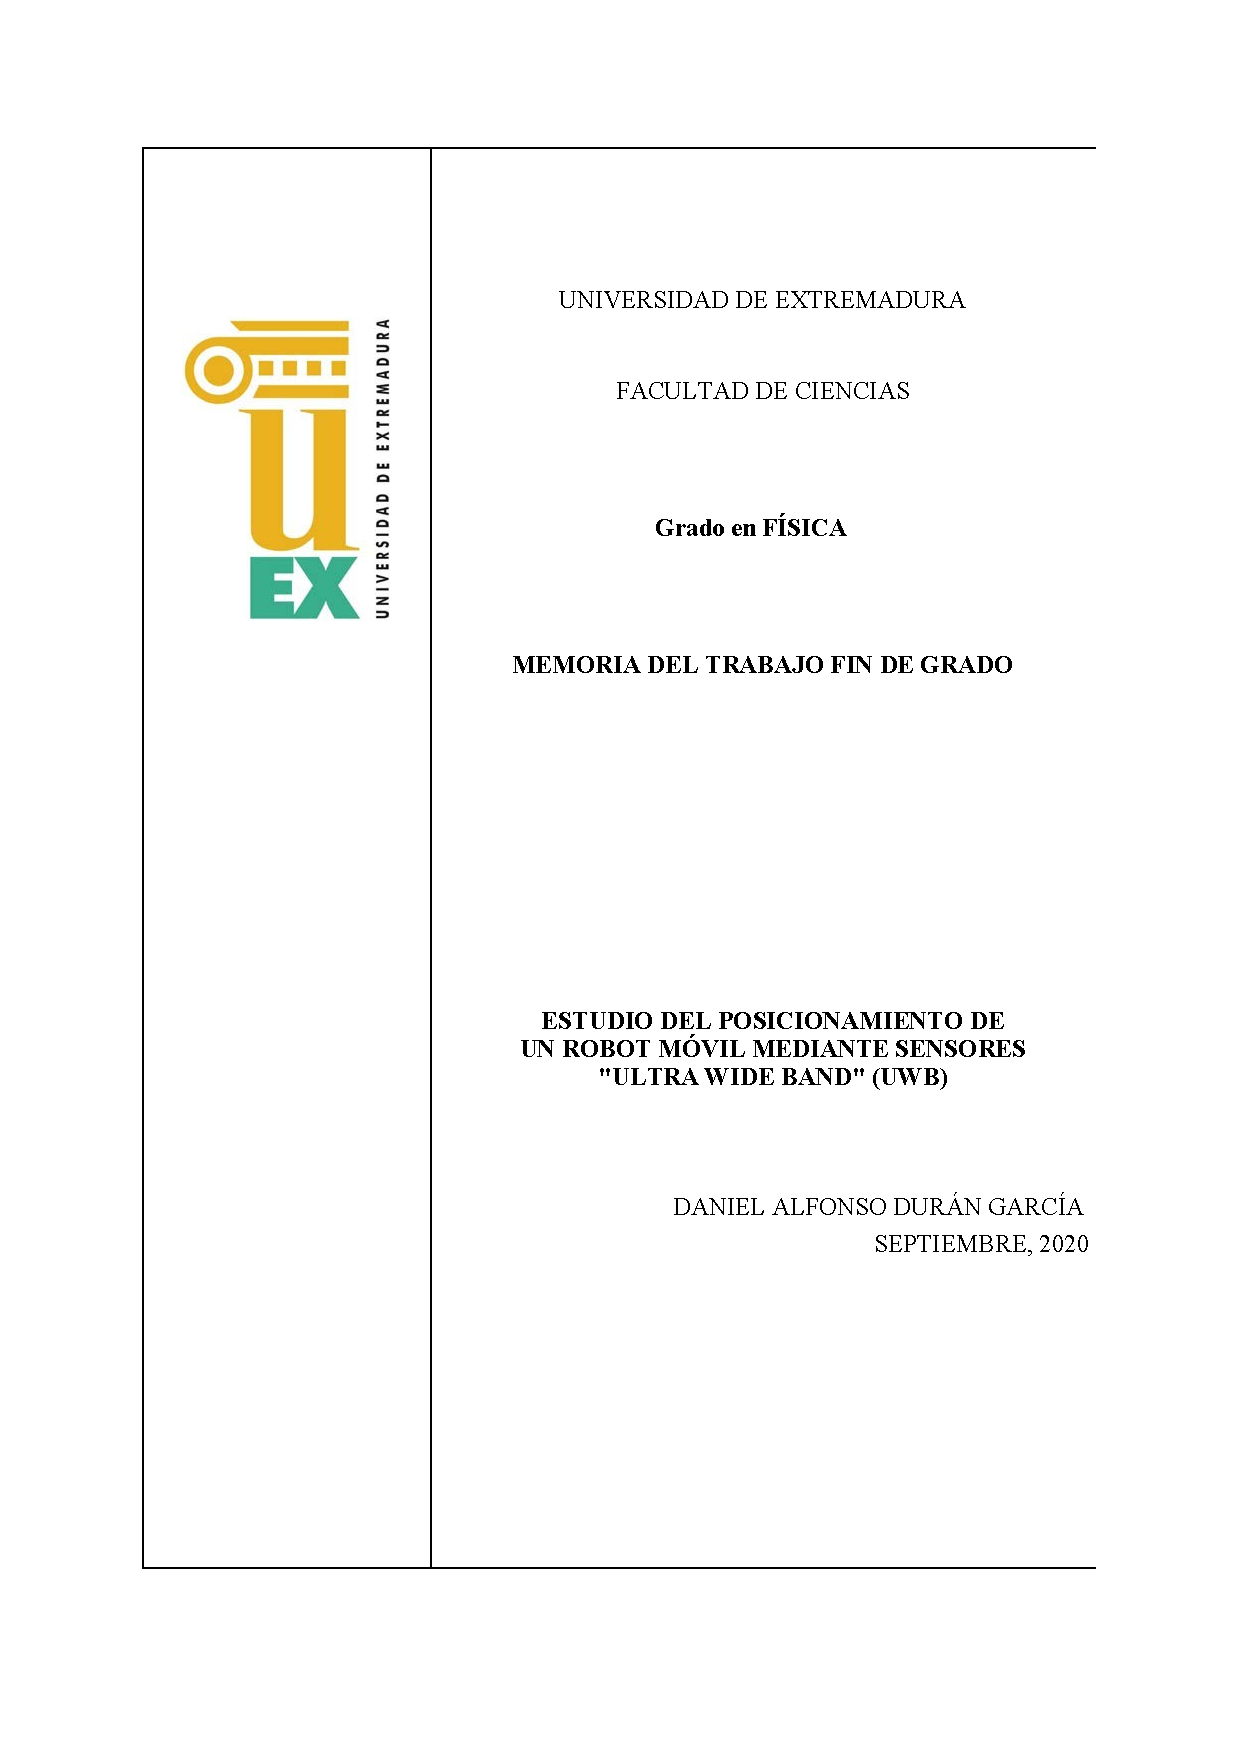
\includepdf[pages=1]{portada.pdf}

\shipout\null %Página en blanco

\pagestyle{empty}
\vspace*{5cm}

Carlos Javier García Orellana, profesor del
Departamento de Ingeniería Eléctrica, Electrónica y Automática de la Universidad de
Extremadura.

INFORMA:

Que D. Daniel Alfonso Durán García ha realizado
bajo su dirección el Trabajo Fin de Grado. Consideran que la memoria reúne
los requisitos necesarios para su evaluación.

\vspace*{1cm}
\begin{center}
Badajoz, día de mes de 2020


\vspace{5cm}
Fdo. Carlos Javier García Orellana
\end{center}

\newpage %Página en blanco
\setcounter{page}{1}
\pagestyle{plain}

\tableofcontents


%------------------------------------------------------------------------------
%                             Resumen
%------------------------------------------------------------------------------

\newpage
\section*{Resumen}

Debido a las limitaciones del uso de sistemas de posicionamiento global en interiores aparecen soluciones parecidas, pero adaptadas a estos ambientes con dimensiones menores y ambientes diferentes.
Dentro de las distintas tecnologías empleadas el Ultra-wide Band, que usa señales de al menos 500MHz de ancho de banda, está ganando poco a poco popularidad por ser una tecnología poco intrusiva y efectiva en un espectro electromagnético muy poblado, con una precisión en el orden del centímetro, pero muy dependiente del entorno donde se emplea.

Así, en este trabajo se plantean dos localizaciones para evaluar, en condiciones de uso ideales y no ideales, la precisión del kit comercial DecaWave MEDK1001 con la ayuda de un robot.
Con varias configuraciones de los sensores en ambos escenarios, se comparó el desempeño del kit en diversas situaciones para determinar cómo afectan los obstáculos a las estimaciones de posición que proporciona.

%------------------------------------------------------------------------------
%                             Abstract
%------------------------------------------------------------------------------

% \newpage
\section*{Abstract}

Given the limitations of the global positioning systems at indoors new solutions have been developed adapted to these situations, with a smaller scale and different backgrounds.
Among the technologies used, Ultra-wide Band, which uses pulses of at least 500MHz bandwidth, has been gaining traction as it is lowly intrusive and highly effective in a saturated electromagnetic spectrum giving a precision in the order of centimeters depending on the scenario.

In this work two locations are chosen, with ideal and non-ideal conditions, to evaluate the precision of the DecaWave MDEK1001 commercial kit using a robot.
Testing various setups in both scenarios, the performance of the kit in several situations was compared to determine how obstacles affect the position estimations it provides.

% Páginas impares.
\let\oldsection\section% Store \section in \oldsection
\renewcommand{\section}{\cleardoublepage\oldsection}% Prepend new \section with \cleardoublepage

%------------------------------------------------------------------------------
%                             Objetivos
%------------------------------------------------------------------------------

% \newpage
% \section{Objetivos}

% En este trabajo se trata de evaluar la capacidad de la tecnología Ultra-wide Band para las tareas de posicionamiento local.
Para este acometido es fundamental tener en cuenta el entorno en el que se intenta conseguir dicho posicionamiento y la disposición de todo el entramado de sensores para encontrar la configuración óptima.

Por ello, los objetivos del trabajo son
\begin{itemize}
    \item Evaluar la precisión de los sensores de Ultra-wide Band en un entorno favorable, de tal manera que es posible encontrar los límites de una forma fácilmente parametrizable y sin incluir fuentes adicionales de error.
    \item Evaluar de nuevo la precisión de los sensores en un segundo escenario menos favorable, con obstáculos que puedan interferir en las tareas de posicionamiento y así poder comprobar cómo afectan estas nuevas variables a los errores en la posición obtenida.
    \item Comparar el desempeño de la tecnología en ambos escenarios, y las discrepancias frente a los valores teóricos.
    \item En ambos casos, realizar tomas de medidas con distintas configuraciones de los sensores, y así poder evaluar cuáles de ellas arrojan mejores resultados y así encontrar el mejor equilibrio entre su desempeño y su complejidad.
\end{itemize}

%------------------------------------------------------------------------------
%                             Introduccion
%------------------------------------------------------------------------------

\newpage
\section{Introducción y objetivos}

El éxito de los sistemas de posicionamiento global como el GPS ha iniciado en los últimos años el desarrollo de tecnologías y experiencias basadas en el control y el seguimiento de la posición de objetos o personas.

En ambientes exteriores y abiertos, la precisión de este tipo de sistemas, con el equipamiento adecuado, puede llegar a ser de centímetros.
No es el caso en situaciones interiores, donde la nula línea de visión directa entre los medidores y los satélites hacen que esta precisión sea imposible, por lo que su uso, en general, es inviable.

Debido a estos inconvenientes han aparecido nuevas técnicas para conseguir un posicionamiento similar, pero de forma local.
Aunque su objetivo es el mismo, los entornos interiores requieren una precisión mayor y tienen, en general, un espectro electromagnético más poblado, por lo que se deben emplear tecnologías distintas compatibles con estos escenarios.

\begin{figure}[H]
    \centering
    \def\svgwidth{1.1\linewidth}
    \input{./fig/general.pdf_tex}
	\caption{Esquema general de un sistema de posicionamiento local.}
    \label{fig:Gen}
\end{figure}

% Con el mismo resultado como objetivo estas tecnologías tienen serias diferencias debido a las circunstancias para las que se desarrollan: entre ellas se encuentran principalmente la precisión requerida, mucho mayor en interiores, o la necesidad de lidiar con un espectro electromagnético más poblado.

\textbf{A diferencia del caso del posicionamiento global, existen dos tipos de algoritmos: unos basados en argumentos geométricos a partir de emisores con posición conocida, y otros consistentes en un mapeado previo de la zona de interés.
Estas técnicas y las tecnologías sobre las que se implementan son las principales diferencias entre las alternativas comerciales disponibles.}

La proliferación de la comunicación inalámbrica ha provocado una saturación en el espectro electromagnético, de tal forma que nuevos usos que puedan emplear este tipo de ondas se vean seriamente afectados por interferencias en la frecuencias en uso.

Aunque su planteamiento se remonta varias decenas de años en el tiempo, es cada vez más habitual la mención al Ultra-wide Band (UWB), una tecnología que usa un espectro de ondas de radio con un ancho de banda superior al 20\% de la frecuencia central o mayor que 500 MHz.

Su gran ancho de banda permite la emisión de pulsos muy cortos en el tiempo y de baja energía, lo que hace que su implantación tenga una alta eficiencia.
Además no requiere diseños complejos para la emisión ni para la recepción de pulsos, con lo que el equipamiento necesario para su uso tendrá en general un bajo coste.

La baja tolerancia que proporciona un uso tan amplio de frecuencias a las interferencias --a diferencia del Bluetooth o Wi-Fi, con canales con ancho de banda mucho más pequeño-- la hacen muy atractiva para su uso masivo teniendo en cuenta que es posible asegurar un buen funcionamiento independientemente del uso simultáneo de otras tecnologías.

El estudio de la precisión disponible del UWB es el principal foco de este trabajo.
La baja potencia de los pulsos usados para el posicionamiento hace que la presencia de obstáculos sea su principal punto débil, con una capacidad de penetración muy baja.

En escenarios con una configuración en la que el objetivo del posicionamiento no tenga línea visión directa de las balizas no será posible tener mediciones excesivamente precisas, y determinar los límites en dichos casos será crítico para evaluar el uso del UWB o de alguna de sus alternativas.

Para automatizar la toma de datos en la medida de lo posible se ha usado un robot en el que colocar el sensor de UWB a posicionar, de tal forma que ha sido posible una toma de datos con un volumen mayor a comparación de una metodología manual.

El robot utilizado ha sido el Turtlebot 2, un pequeño robot con fines educativos que permite el uso de cámaras y sensores láser para labores de movimiento autónomo, de tal forma que permite un movimiento total en un entorno controlado.
Aunque es posible una navegación libre a partir de los sensores mencionados, para este trabajo se creó un mapa de los dos escenarios en los que se produjo la toma de medidas para que su posicionamiento local fuese lo más preciso posible.

Dicho robot fue empleado en dos escenarios para poder comparar el desempeño de los sensores de UWB en dos situaciones distintas.
Así, en la elección los dos escenarios se primó la posibilidad de comparar una situación ideal, con visión directa y distancias cortas; y una situación más parecida a un uso habitual, con un escenario en el que, en ocasiones, pueda haber obstáculos que dificulten el traslado de la señal de UWB.

La primera toma de medidas se llevó a cabo en uno de los laboratorios de los Institutos Universitarios de Investigación en el que se disponía de una superficie amplia y libre; la segunda localización tuvo lugar en el edificio B de la Facultad de Física, donde por razones estructurales existen varias columnas en sus plantas y en ocasiones aparece un leve tráfico de personas.

Así, los objetivos de este trabajo son
\begin{itemize}
    \item Evaluar la precisión de los sensores de Ultra-wide Band en un entorno favorable, de tal manera que es posible encontrar los límites de una forma fácilmente parametrizable y sin incluir fuentes adicionales de error.
    \item Evaluar de nuevo la precisión de los sensores en un segundo escenario menos favorable, con obstáculos que puedan interferir en las tareas de posicionamiento y así poder comprobar cómo afectan estas nuevas variables a los errores en la posición obtenida.
    \item Comparar el desempeño de la tecnología en ambos escenarios, y las discrepancias frente a los valores teóricos.
    \item En ambos casos, realizar medidas con distintas configuraciones de los sensores para evaluar cuáles de ellas arrojan mejores resultados y así encontrar el mejor equilibrio entre su desempeño y su complejidad.
\end{itemize}

%------------------------------------------------------------------------------
%                             Antecedentes
%------------------------------------------------------------------------------

\newpage
\section{Antecedentes}

\subsection{Técnicas de estimación de la posición}

Existen dos alternativas para estimar la posición de un objetivo a partir de la posición conocida de un cierto número de balizas con coordenadas conocidas: la primera, denominada \textit{fingerprinting}, se basa en la obtención de un modelo de posicionamiento a partir de la medición de la potencia de las balizas; la segunda, obtiene las estimaciones a partir de técnicas geométricas \cite{MAIN}.

\subsubsection{\textit{Fingerprinting}}

La primera de las opciones para estimar la posición de un objetivo se basa en la medición de la potencia de la señal recibida desde cada una de las balizas.

Esta técnica requiere un mapeado previo de la zona de interés que permita obtener un modelo contra el que comparar en su uso posterior.
La dependencia en un modelo previo provoca que cualquier modificación del entorno --como por ejemplo tránsito de personas-- hace que la estimación sea en el mejor de los casos ligeramente distinta y en el peor, imposible.

La comparación contra el modelo hace uso de algoritmos de \textit{machine learning} como \textit{k-nearest-neighbor} o \textit{support vector regression}, que buscan minimizar la diferencia entre las medidas y dicho modelo. 
Requieren, de forma general, una capacidad computacional mayor a las alternativas geométricas, por lo que son usados habitualmente en entornos con obstáculos estáticos y sin demasiadas modificaciones, donde su ventaja es significativa.

\subsubsection{Técnicas geométricas}

La multiliteración -- también llamada \textit{triliteración} en el caso de usar tres puntos de referencia -- es una técnica para conocer la posición de un objetivo con argumentos geométricos.

Se basa en la búsqueda de la intersección de ciertas áreas a partir de la posición de varias balizas con posición conocida.
Estas áreas están definidas por distancias o ángulos a las balizas de referencia, valor obtenible con distintas técnicas.

En general, la posición del objetivo vendrá dado, en $n$ dimensiones, por
\begin{equation}\label{eq:geom}
    \vb{r} = \vb{f}(x_1, x_2, \ldots, x_n) + \vb{n}
\end{equation}
donde $\vb{f}$ será la función característica de cada algoritmo y $\vb{n}$ un vector que representa el ruido de la señal, con un valor medio nulo.

% \subsubsubsection{Límites teóricos}

% Al plantear la ecuación general de las técnicas geométricas \eqref{eq:geom} se introdujo un término relacionado con el ruido relacionado con la generación y el traslado de la señal desde la baliza hasta el objetivo.
% Este ruido tiene un carácter aleatorio, por lo que su caracterización habitual es la de ruido blanco gaussiano, con valor medio cero.

Este ruido está relacionado con la generación y el traslado de la señal desde la baliza hasta el objetivo y tiene un carácter aleatorio, por lo que su caracterización habitual es la de ruido blanco gaussiano, con valor medio cero.

Esta caracterización, unida al muestreo discreto de la señal por parte de los dispositivos electrónicos, resulta en un límite en la precisión del posicionamiento, incluso en los casos más ideales.

El límite más usual viene dado por la cota inferior de Cramer-Rao (CRLB), definido como la traza de la matriz de Fisher inversa.
La matriz de Fisher se construye, en el caso de la parametrización del ruido con características gaussianas, como \cite{Xbook}
\begin{equation}
    [\mathcal{I}(\bm{\theta})]_{ij} = \frac{1}{\sigma^2} \sum_{n=0}^{N=1} \pdv{s[n,\bm{\theta}]}{\theta_i}\pdv{s[n,\bm{\theta}]}{\theta_j}
\end{equation}
donde $\bm{\theta}$ indica el vector con los parámetros a evaluar, $\sigma$ la desviación del ruido blanco gaussiano, $N$ el número de balizas utilizadas y $s[n,\bm{\theta}]$ la señal emitida por la baliza $n$, sin ningún ruido.

Así, la varianza de cada uno de los parámetros a estimar vendrá dada como
\begin{equation}
    \sigma^2(\theta_i) \geq [\mathcal{I}(\bm{\theta})^{-1}]_{ii}
\end{equation}

% Así, se obtiene un límite para cada tipo de técnica, ya que se medirán distintos parámetros en cada una de ellas, dados por:
% \begin{equation}
%     \text{CRLB}
%     \begin{cases}
%         \displaystyle\frac{1}{8\pi^2 \text{SNR} \beta^2} & \text{TOA y TDOA} \\
%         \\[2pt]
%         \displaystyle\frac{1}{2\pi^2 \text{SNR} \beta^2 N(N^2-1)d\cos(\theta)} & \text{AOA} \\
%         \\[2pt]
%         \displaystyle\frac{\ln(10)\sigma_{sh}d}{10n} & \text{RSSI} \\
%     \end{cases}
% \end{equation}
% donde $\beta$ denota el ancho de banda efectivo dado por
% \begin{equation}
%     \beta^2 = \frac{\int_{-\infty}^{\infty} \omega^2 \abs{S(\omega)}^2\dd{\omega}}{\int_{-\infty}^{\infty} \abs{S(\omega)}^2\dd{\omega}}
% \end{equation}
% con $S(\omega)$ como la transformada de Fourier de la señal $s(t)$.

% SNR es la razón entre la señal y el ruido --\textit{signal-to-noise ratio}, en inglés--, de la que se tiene una relación inversamente proporcional.

% Para los casos de AOA y TOA, el CRLB toma valores demasiado bajos cuando el SNR es muy bajo.
% Por ello en dichas situaciones es habitual el uso de la cota inferior de Ziv-Zakai (ZZLB) \cite{soganzi}, que no sufre este problema, aunque no siempre es posible evaluar de forma analítica.

% Con argumentos geométricos es posible construir una serie de algoritmos basados en la posición conocida de ciertas balizas.

\subsubsubsection{Tiempo de llegada (TOA)}

El primer algoritmo considera una velocidad de transmisión conocida y una línea de visión directa entre las balizas y el objetivo.
Teniendo en cuenta que el medio de propagación será el aire, la velocidad de la señal será la velocidad de la luz en el caso de ondas electromagnéticas.
Esta velocidad no tendrá variaciones significativas al cambiar la zona de interés, por lo que será válida para prácticamente cualquier escenario.

Denotando al objetivo como OBJ y con tres balizas llamadas $B_i$ con $i=1,2,3$, la distancia recorrida por cada señal hasta el objetivo será \footnote{Durante todo el desarrollo de la teoría de posicionamiento en esta sección se supondrá un sistema bidimensional. Esto no puede ser así en la implementación \textit{real}, pero teniendo en cuenta que en el posicionamiento local se trata con sistemas euclídeos la adición de la tercera componente en todos los cálculos es trivial.}
\begin{equation}\label{eq:TOA}
    \begin{aligned}
        d_i &= c(t_i) = c(\tau_i - t_0) \\
        &= \sqrt{(x_i - x)^2 + (y_i - y)^2} + ct_0
    \end{aligned}
\end{equation}
siendo $t_0$ el instante en el que la baliza $i$ emitió el pulso.
Así, la función característica de este algoritmo será, en dos dimensiones
\begin{equation}
    f_i(x, y) = \sqrt{(x_i - x)^2 + (y_i - y)^2}
\end{equation}
para cada baliza, definiendo una circunferencia de radio $d_i$ como se muestra en la Figura~\ref{fig:TOA}.

\begin{figure}[H]
    \centering
    \def\svgwidth{0.6\linewidth}
    \input{./fig/TOA.pdf_tex}
	\caption{Posicionamiento por tiempo de vuelo (TOA).}
    \label{fig:TOA}
\end{figure}

A partir de las ecuaciones de \eqref{eq:TOA} la posición de OBJ será \cite{Zafer}
\begin{equation}
    \begin{aligned}
        x = \frac{(y_2-y_1)\gamma_1 + (y_2-y_3)\gamma_2}{2[(x_2-x_3)(y_2-y_1) + (x_1 - x_2)(y_2 - y_3)]}\\
        y = \frac{(x_2-x_1)\gamma_1 + (x_2-x_3)\gamma_2}{2[(x_2-x_1)(y_2-y_3) + (x_2 - x_3)(y_1 - y_2)]}\\
    \end{aligned}
\end{equation}
donde
\begin{equation}
    \begin{aligned}
        \gamma_1 = x_2^2 - x_3^2 + y_2^2 - y_3^2 + d_3^2 - d_2^2 \\
        \gamma_2 = x_1^2 - x_2^2 + y_1^2 - y_2^2 + d_2^2 - d_1^2 \\
    \end{aligned}
\end{equation}

En este algoritmo es crítica una correcta sincronización entre los relojes de las balizas y el objetivo.
Es posible minimizar este problema usando solo uno de los puntos para medir la distancia esperando una reemisión: emitiendo, desde una de las balizas o el objetivo, un pulso y esperando una respuesta similar del objetivo, con lo que el tiempo total será el doble del tomado por la señal original en llegar a la posición requerida.

El CRLB en el caso de TOA viene dado por \cite{Xbook}
% Esta precisión vendrá por tanto dada por el nivel de ruido en la señal, con la expresión
\begin{equation}\label{eq:CRLB_TOA}
    \text{CRLB} = \sigma^2(\tau) \geq \frac{1}{8\pi^2\text{SNR}\beta^2}
\end{equation}
donde $\tau$ es la distancia estimada y $\beta$ el ancho de banda efectivo dado por
\begin{equation}
    \beta^2 = \frac{\int_{-\infty}^{\infty} \omega^2 \abs{S(\omega)}^2\dd{\omega}}{\int_{-\infty}^{\infty} \abs{S(\omega)}^2\dd{\omega}}
\end{equation}
con $S(\omega)$ como la transformada de Fourier de la señal $s(t)$.

SNR es la razón entre la señal y el ruido --\textit{signal-to-noise ratio}, en inglés--, de la que se tiene una relación inversamente proporcional.
Es decir, la relación esperada: el SNR proporciona la relación entre la energía de la señal y la energía del ruido que la corrompe, así que un valor mayor indica menos ruido y por tanto una incertidumbre menor en la intersección de los pulsos de las balizas.

En este caso, el CRLB toma valores demasiado bajos cuando el SNR es muy bajo.
Por ello en dichas situaciones es habitual el uso de la cota inferior de Ziv-Zakai (ZZLB) \cite{soganzi}, que no sufre este problema, aunque no siempre es posible evaluar de forma analítica.

\subsubsubsection{Diferencia de tiempo de llegada (TDOA)}

Para eliminar la sincronización de relojes entre las balizas y el objetivo es posible usar también la diferencia temporal entre las señales de las balizas, teniendo así independencia en el sistema del objetivo.
Aunque se consiga la independencia del reloj del objetivo, esta configuración sigue requiriendo que los relojes de las balizas estén sincronizados entre sí.

Así, la diferencia entre las distancias de las señales de dos balizas, teniendo en cuenta los tiempos en la llegada de la señal de dichas balizas será
\begin{equation}\label{eq:TDOA}
        d_{ij} = c(t_i - t_j) = c \left[  (\tau_i + t_0) - (\tau_j + t_0)\right] = c(\tau_i - \tau_j)
\end{equation}
válida para $i=1,2,3$ y $j=1,2,3$ con $i \neq j$.
Así, la función característica de este algoritmo será
\begin{equation}\label{eq:funcion_TDOA}
    f_i(x,y) = \sqrt{(x_i - x)^2 + (y_i - y)^2} - \sqrt{(x_j - x)^2 + (y_j - y)^2}
\end{equation}
para cada baliza $i$ respecto de cualquiera $j$ de las otras.

\begin{figure}[H]
    \centering
    \def\svgwidth{0.55\linewidth}
	\input{./fig/TDOA.pdf_tex}
    \caption{Posicionamiento por diferencia tiempo de vuelo (TDOA)}
    \label{fig:TDOA}
\end{figure}

La función característica \eqref{eq:funcion_TDOA} hace que se definan parábolas en torno a cada una de las balizas, como se muestra de forma cualitativa en la Figura~\ref{fig:TDOA}.

Así, tomando la baliza 1 como referencia tenemos que las coordenadas del objetivo vienen dadas por el sistema de ecuaciones
\begin{equation}
    \begin{cases}
        d_{12} &= \sqrt{(x_1 - x)^2 + (y_1 - y)^2} - \sqrt{(x_2 - x)^2 + (y_2 - y)^2} \\
        d_{13} &= \sqrt{(x_1 - x)^2 + (y_1 - y)^2} - \sqrt{(x_3 - x)^2 + (y_3 - y)^2} \\
    \end{cases}
\end{equation}
con el que se obtiene de forma general dos soluciones para el posicionamiento: en la mayoría de casos una de ellas será un punto fuera de los límites del recinto en que se trabaja por lo que se elegirá el más cercano a las balizas colocadas.

En el caso de TDOA el CRLB tiene la misma expresión que en el TOA \eqref{eq:CRLB_TOA}, teniendo en cuenta que el ruido añadido a las señales de las balizas tendrá la misma caracterización.

\subsubsubsection{Intensidad de la señal recibida (RSSI)}

Para evitar problemas con la sincronización de los relojes necesaria en las técnicas anteriores es posible aprovechar el decaimiento de la intensidad de la señal con la distancia según la relación
\begin{equation}\label{eq:RSSI}
    p(r) = p(r_0) - 10n\log(\frac{r}{r_0})
\end{equation}
donde $p(r_0)$ y $p(r)$ son la intensidad de la señal en el origen y el objetivo respectivamente y $n$ el exponente de atenuación de la señal.

Esta técnica es muy susceptible ante el ruido ambiental y las posibles interferencias que puedan ocurrir entre las señales de distintas balizas o de fuentes externas.
La disposición geométrica es similar a la vista en la técnica de tiempo de llegada (Figura~\ref{fig:TOA}), donde a partir de una medición de la señal de una baliza es posible definir una circunferencia de centro en dicha baliza y radio dado por \eqref{eq:RSSI}.

A diferencia de los casos de TOA y TDOA el CRLB en esta técnica es independiente del ancho de banda de la señal, dado por \cite{MAIN}
\begin{equation}\label{eq:CRLB_RSSI}
    \sigma^2(d_i) = \frac{\ln(10)\sigma_{sh}d}{10n}
\end{equation}
donde $\sigma_{sh}$ indica la desviación estándar del desvanecimiento de la señal.

La independencia de las cotas inferiores del ancho de banda de la señal hacen que esta técnica no aproveche la principal ventaja que da el UWB, por lo que su uso se restringe a otras tecnologías.

\subsubsubsection{Ángulo de llegada (AOA)}

Otra opción para evitar la sincronización de los relojes entre las balizas consiste en usar el ángulo de incidencia de la señal en el objetivo como se muestra en la Figura~\ref{fig:AOA}, de tal forma que, para una baliza $B_i$ dicho el objetivo se encuentra en la posición
\begin{equation}
    \label{eq:AOA}
    \begin{aligned}
        x = d_i \cos(\phi_i) + x_i \\        
        y = d_i \sin(\phi_i) + y_i         
    \end{aligned}
\end{equation}
por lo que la función característica de este algoritmo será la distancia de cada baliza al objetivo, a partir de \eqref{eq:AOA}
\begin{equation}
    f_i = \arctan(\phi_i) = \arctan(\frac{y-y_i}{x-x_i})
\end{equation}

\begin{figure}[H]
    \centering
    \def\svgwidth{0.6\linewidth}
	\input{./fig/AOA.pdf_tex}
    \caption{Posicionamiento por ángulo de llegada (AOA).}
    \label{fig:AOA}
\end{figure}
Esta técnica requiere el uso de antenas direccionales, lo que hace que aumente el coste de su implantación.

En este caso solo necesitamos el ángulo respecto a las balizas, por lo que su implantación será más adecuada en situaciones en las que el cálculo de la distancia entre objetivo y balizas no es fiable o como apoyo o correción junto con TOA o TDOA.

Para el AOA el CRLB, que nos dará el mínimo de varianza para el ángulo de incidencia vendrá dado, en el caso de balizas colocadas a lo largo de un eje de la forma mostrada en la Figura~\ref{fig:AOA} por \cite{Xbook, shim2018}
\begin{equation}
    \sigma^2(\phi) = \frac{c^2}{2\pi^2 \text{SNR} \beta^2 N(N^2-1)d\cos(\phi)}
\end{equation}
donde $N$ indica el número de balizas utilizadas y $d$ la distancia entre ellas.

\subsubsection{Mitigación en casos no ideales}

En el planteamiento de los algoritmos geométricos se suponía una línea de visión directa entre las balizas y el objetivo para determinar los parámetros de interés, pero en condiciones reales esta suposición no siempre podrá ser respetada.

La presencia de obstáculos que impidan un trayecto de la señal parametrizable o generen rebotes en la zona de interés pueden provocar un posicionamiento erróneo o, en el peor de los casos, imposible.

Para mitigar la modificación en la señal en estos casos se recurre a técnicas estadísticas que se dividen en dos grupos: técnicas paramétricas, en las que se realiza un ajuste del error a una distribución de probabilidad conocida, y técnicas no paramétricas, en la que no se asume ninguna distribución a priori.

% \subsubsubsection{Técnicas paramétricas}

% El primer grupo de técnicas consiste en aplicar argumentos estadísticos de tal forma que es posible ajustar la señal recibida en el objetivo a una cierta función de probabilidad, de tal manera que es posible filtrar en cierta medida el ruido y las interferencias que acompañan al pulso original \cite{Zafer}.

% Definiendo como $\bm{\theta} = [x,y,\lambda]^T$ el vector que contiene los parámetros de la distribución, podemos establecer una función de probabilidad del ruido introducido en la señal como
% \begin{equation}
%     p(r|\bm{\theta})
% \end{equation}
% indicando la probabilidad de densidad de $r$ conociendo $\bm{\theta}$.

% A partir de esta función de probabilidad es posible aplicar estimadores Bayesianos, principalmente el mínimo error cuadrático medio (MMSE, \textit{minimum mean square error}) definido como
% \begin{equation}\label{eq:MMSE}
%     \hat{\bm{\theta}}_{\text{MMSE}} = E\{\bm{\theta}|\vb{r}\}
% \end{equation}
% con $E\{\bm{\theta}|\vb{r}\}$ como el valor esperado de $\bm{\theta}$ dado $\vb{r}$, o el estimador de máximos a posteriori (MAP), definido como
% \begin{equation}
%     \hat{\bm{\theta}}_{\text{MAP}} = \argmax_{\bm{\theta}} p(\bm{\theta}|r)
% \end{equation}

% A partir del teorema de Bayes tenemos que
% \begin{equation}
%     p(\bm{\theta}|r) = \frac{p(r|\bm{\theta})p(\bm{\theta})}{p(r)}
% \end{equation}
% por lo que maximizar $p(\bm{\theta}|r)$ equivale a maximizar $p(r|\bm{\theta})p(\bm{\theta})$ y así tenemos que la estimación a posteriori será \cite{Xbook}
% \begin{equation}\label{eq:MAP}
%     \hat{\bm{\theta}}_{\text{MAP}} = \argmax_{\bm{\theta}} p(r|\bm{\theta})p(\bm{\theta})
% \end{equation}
% o de forma equivalente
% \begin{equation}
%     \hat{\bm{\theta}}_{\text{MAP}} = \argmax_{\bm{\theta}} [\ln(p(r|\bm{\theta})) + \ln(p(\bm{\theta})) ]
% \end{equation}
% con $p(\bm{\theta})$ como la información a priori de la distribución de probabilidad del ruido de la señal.

% En el caso de las señales utilizadas, dicha distribución a priori es a veces exponencial si en el camino recorrido se espera un gran número de obstáculos o, de forma más habitual, de tipo gaussiano.

% En los casos en los que esta información a priori no es conocida es posible utilizar un estimador por máxima similitud de tal forma que la estimación será
% \begin{equation}\label{eq:ML}
%     \hat{\bm{\theta}}_{\text{ML}} = \argmax_{\bm{\theta}} p(r|\bm{\theta})
% \end{equation}
% donde la función de similitud vendrá dada por
% \begin{equation}
%     p(r|\bm{\theta}) = p_n(\vb{r} - \vb{f}|\bm{\theta})
% \end{equation}
% a partir de \eqref{eq:geom}.
% $p_n(\cdot | \bm{\theta})$ indica la función de probabilidad del vector de ruido condicionada por los parámetros de $\bm{\theta}$.

% En el caso de componentes de ruido independientes esta función de probabilidad será
% \begin{equation}
%     p_n(\vb{r} - \vb{f}|\bm{\theta}) = \prod_i^{N} p_{n_i}(r_i - f_i|\bm{\theta})
% \end{equation}
% donde, como en el caso de la estimación a posteriori, la parametrización habitual es la de una distribución gaussiana para cada componente.

% Esta asunción es generalmente válida en el caso de TOA, AOA o RSS, donde el ruido de cada baliza no interferirá en los otros.
% No será el caso de las estimaciones con TDOA, donde en el cálculo de los parámetros de interés intervendrá el ruido generado en la señal de al menos dos balizas, por lo que es necesario establecer una mínima correlación.

% Cabe recordar que en los casos ideales ya se tenía en consideración un cierto ruido en el transporte de la señal.
% En los casos no ideales tratados ahora --como puede ser por ejemplo la presencia de obstáculos-- no se deja de considerar aquella primera aproximación, por lo que las funciones de probabilidad tratadas en total tendrán dos componentes: el del caso ideal más una nueva componente fruto del nuevo entorno.

% \subsubsection{Técnicas no paramétricas}

% En los casos en los que no es posible conocer una distribución a priori del ruido ni modelizarlo con una cierta distribución de probabilidad se recurre habitualmente a un ajuste de mínimos cuadrados.
% Así, definiendo $\vb{z} = [x,y]^T$ como la posición desconocida del objetivo, $\vb{z}_i$ la posición de la baliza $i$ y $r_i$ la distancia obtenida entre el objetivo y dicha baliza se tiene \cite{MAIN}
% \begin{equation}
%     \hat{\vb{z}} = \argmin_{\vb{z}} \sum_i(r_i - ||\vb{z} - \vb{z}_i||)^2
% \end{equation}
% con $||\vb{z} - \vb{z}_i||$ como el módulo euclídeo indicando la distancia entre cada baliza y el objetivo.

% En el caso de mediciones con TDOA este módulo debe ser modificado para adecuarse a la naturaleza hiperbólica de la curvas de las que se busca la intersección.

% En condiciones reales los ajustes de mínimos cuadrados se ven muy contaminados por los escenarios sin visión directa y las incertidumbres de los sensores, por lo que habitualmente se usan ciertos pesos en las medidas de cada una de las balizas para favorecer a aquellas en las que la recepción es más favorable.

\subsection{Tecnologías}

Todos los algoritmos geométricos mencionados necesitan un soporte físico para determinar las variables con las que determinar la posición del objetivo que requieren, para lo que es posible el uso de varias tecnologías, como se recoge en \cite{COMP}, de donde procede toda la información de esta sección.

\subsubsection{Sonido}

Una primera propuesta puede ser el uso de ondas de sonido, normalmente fuera del rango de audición humano. Dependiendo de la frecuencia utilizada son referidos a veces como \text{ultrasonidos}.

La baja velocidad de propagación en el aire hace que la incertidumbre en la medida de los tiempos de llegada sea muy baja, por lo que su uso se asocia casi exclusivamente a TOA y TDOA.

Esta tecnología tiene su principal punto débil en la dependencia de la propagación del sonido con la temperatura y la humedad del aire: la precisión ganada por la baja velocidad de propagación se ve compensada con un rango máximo muy bajo, lo que hace que su implantación en entornos amplios no sea óptimo.
Además, el equipamiento necesario tiene un coste mayor al de sus alternativas, por lo que su uso se restringe actualmente a situaciones concretas.

\subsubsection{Luz}

La popularización de la iluminación LED, capaz de cambiar la intensidad de emisión en tiempos muy cortos ha provocado el desarrollo de tecnologías que modulen información a tasas de tiempo mucho más altas de la que el ojo humano puede captar.

Su principal ventaja es la posibilidad de aprovechar las infraestructuras de iluminación ya existentes en ambientes interiores, aunque esta tecnología es muy dependiente de las condiciones en dichas situaciones.

La desventaja más directa es su total reflexión en paredes u objetos opacos, lo que hace que la atenuación sea importante en interiores donde la disposición desfavorezca una iluminación uniforme o simplemente un tráfico intenso de personas.
Además, es muy sensible a fuentes externas como luz solar.

\subsubsection{Visión por computador}

El desarrollo en los últimos años de técnicas para el reconocimiento de imágenes ha hecho posible la obtención de técnicas de posicionamiento con cámaras.

Esta técnica ha tenido especial auge en el campo de vehículos autónomos, aunque su uso se complementa de forma habitual con otras tecnologías al necesitar buenas condiciones lumínicas para su correcto funcionamiento.

Al igual que en el caso de la luz, su principal ventaja reside en el aprovechamiento de la infraestructura ya existente.
En este caso es posible utilizar una tecnología ya asentada y madura sin realizar ninguna modificación sin más que usar cámaras con la resolución suficiente para los distintos casos de uso.

\subsubsection{Campo magnético}

Aunque hay algunos trabajos que desarrollan el sistema de posicionamiento sobre un campo magnético artificial, la mayoría de aplicaciones se basan en el campo magnético terrestre para determinar la posición del objetivo.

Estas técnicas requieren un estudio previo para determinar la intensidad de dicho campo magnético terrestre a lo largo del espacio en los que implementar el posicionamiento, aunque tras ello el equipamiento necesario es mínimo al requerir únicamente un magnetómetro.

Este tipo de técnicas tiene una precisión muy baja, en torno a metros, y es muy susceptible a cualquier modificación del campo magnético sobre el que se realizó el estudio previo por lo que su aplicación se reduce a situaciones muy concretas.

\subsubsection{Wi-Fi}

En el espectro electromagnético las señales de Wi-Fi son también una alternativa a la hora de determinar distancias por el decaimiento de su intensidad con la distancia.
Su atractivo principal es, como en otras tecnologías, el aprovechamiento de las infraestructuras y el desarrollo ya existente.

Aunque también es posible su uso con TOA y AOA, su uso principal se restringe a técnicas de \textit{fingerprinting}, ya que habitualmente los puntos de acceso Wi-Fi usados para la conexión a internet no suelen superar la unidad por planta o edificio.

Esta escasez de balizas es la principal desventaja: en su uso original un solo emisor puede dar servicio a multitud de dispositivos en una planta o incluso un edificio, por lo que lo habitual será encontrar numerosos obstáculos entre emisor y objetivo.
Colocar más balizas puede añadir interferencias entre las señales teniendo en cuenta que los canales disponibles tienen un ancho de banda bajo.

Además, el uso extendido de esta tecnología inalámbrica hace que su espectro esté ya, en algunas ocasiones, saturado.
Su precisión en ambientes ideales está en torno al metro, así que podría ser una buena opción en entornos abiertos o con pocas redes que puedan causar interferencias.

\subsubsection{Bluetooth}

En el caso del Bluetooth nos encontramos de nuevo con una tecnología con una gran infraestructura ya existente teniendo en cuenta que su uso en teléfonos móviles se da desde hace más de una década.

Entre las distintas generaciones se encuentra un protocolo llamado Bluetooth Low Energy (BLE) centrado en obtener un funcionamiento con el mínimo gasto energético posible, lo que lo hace idóneo para usar como sistema para localización como el que se trata en este trabajo.

Técnicamente comparte el mismo rango de frecuencias con el Wi-Fi y las técnicas de posicionamiento son en general parecidas, aprovechando el decaimiento de la señal con técnicas de \textit{fingerprinting}.
Pero a diferencia del Wi-Fi, la baja energía de los emisores BLE permiten la colocación de un número mayor de balizas, lo que abre la puerta al uso de algoritmos de multiliteración.

Los mejores resultados sobre esta tecnología arrojan una precisión entre 1 y 3 metros, aunque estos resultados dependen en gran medida del número de balizas empleadas.

\subsubsection{Otras tecnologías}

Además de los soportes físicos ya mencionados, existe un enorme abanico de otras tecnologías.
La más ampliamente usada y no mencionada se encuentra en el espectro electromagnético dedicado a las redes móviles, aunque las grandes distancias a las que se encuentran las balizas --torres de comunicación en este caso-- hace que la precisión, en las mejores ocasiones, se encuentre en torno a los 50 metros, inviable para una localización en interiores.

Es posible que el desarrollo de nuevas generaciones de este tipo de redes como el 5G permitan tener una mayor precisión para permitir su uso.

Entre otras alternativas se encuentran también de comunicaciones a muy corta distancia como el \textit{Near-Field Communication} (NFC), aunque este sistema requiere una participación activa del objetivo --debe acercarse mucho a alguna de las balizas-- y no permite localización de objetos en movimiento.

\subsection{Ultra-Wide Band}

El Ultra-Wide Band (UWB) se define como una emisión de radiofrecuencia con un ancho de banda de al menos 500 MHz o más del 20\% de la frecuencia central.
Su definición técnica se recoge en el estándar 802.15.4 del IEEE junto con otras redes inalámbricas de área personal.

Los canales usados y las potencias permitidas tienen distintas legislaciones según el país que se trate.
En el caso de Europa, la regulación del Instituto Europeo de Normas de Telecomunicaciones (ETSI) permite emisiones en los rangos de frecuencia $3.1 - 4.8~\si{\giga\hertz}$, destinado a localización de servicios de emergencia y  $6.0 - 9.0~\si{\giga\hertz}$ para localización general \cite{UWB_regs}.

\subsubsection{Ventajas}

Las cotas de error inferiores en las técnicas de TOA y TDOA tenían una dependencia inversa respecto al ancho de banda de la señal utilizada, como se indicaba en \eqref{eq:CRLB_TOA}.
Por ello la principal característica del UWB, su gran ancho de banda, le proporciona una gran ventaja en su empleo para servicios de posicionamiento a partir de dichas técnicas, siendo su uso principal y el discutido en este trabajo.
Aunque no es el único, ya que también permite la transmisión de datos de una forma rápida y puede llegar a ser una alternativa en este ámbito.

El espectro tan amplio de frecuencia provoca que el decaimiento de la señal, dependiente de la frecuencia, sea fácilmente identificable al estar formado de componentes que sufren este hecho de forma acusada.

Además, un gran ancho de banda permite el uso de pulsos muy cortos en el tiempo, dando una gran resolución temporal.
Teniendo en cuenta que la alta velocidad de transporte de ondas electromagnéticas, la posibilidad de acortar la duración de cada pulso es fundamental para conseguir una alta precisión en el tiempo.
En la Figura~\ref{fig:forma_pulsos} se muestra una comparación cualitativa de este fenómeno.

\begin{figure}[H]
    \begin{subfigure}[b]{.5\textwidth}
      \centering
      \def\svgwidth{0.8\linewidth}
      \input{fig/pulso_tiempo.pdf_tex} 
      \caption{Tiempo}
      \label{fig:forma_pulsos_tiempo}
    \end{subfigure}
    \begin{subfigure}[b]{.5\textwidth}
      \centering
      \def\svgwidth{0.8\linewidth}
      \input{fig/pulso_frec.pdf_tex}
      \caption{Frecuencia}
      \label{fig:forma_pulsos_frec}
    \end{subfigure}
    \caption{Comparación cualitativa entre pulsos con menor ancho de banda, más duraderos en el tiempo (rojo) y con mayor ancho de banda y menor duración temporal (negro).}
    \label{fig:forma_pulsos}
  \end{figure}

En el caso de que se produzca propagación multicamino, en la que los rebotes creen nuevos frentes de onda, la resolución del camino principal se vuelve sencilla teniendo en cuenta que el espacio adicional que recorran las trayectoria sin visión directa --fruto de la reflexión en paredes u obstáculos-- hacen que estos caminos secundarios se verá rápidamente desfavorecidos.

Además, el amplio ancho de banda hace que las interferencias entre los propios pulsos fruto de los distintos caminos sean mínimas, nulas si el tiempo de propagación adicional supera el periodo entre la emisión de dos pulsos.

Este último hecho es muy probable en el caso del UWB, como se comentó anteriormente al emitir pulsos muy cortos en el tiempo.
Además, el tiempo de transmisión de un pulso viene dado por\cite{MAIN}
\begin{equation}
    T_{tx} = \left(N_d + \frac{N_d}{N_{mP}N_{0}N_d} \right) T_b T_{pr}
\end{equation}
donde $N_d$, $N_{mP}$ y $N_{0}$ indican los tamaños de datos, tasa máxima y \textit{overhead} respectivamente;
mientras que $T_b$ y $T_{pr}$ indican la duración y el tiempo de propagación de cada bit, respectivamente.

Si el tiempo de propagación es inversamente proporcional a la tasa de datos, muy amplia en el caso del UWB, dicho tiempo de propagación será por tanto muy bajo, lo que no solo evita las interferencias sino que permite una resolución temporal muy alta.

La tasa de datos viene dada por capacidad de un canal, dada en bits/sec como\cite{MAIN}
\begin{equation}
    C = B\log_2(1 + \text{SNR})
\end{equation}
siendo $B$ el ancho de banda de dicho canal y considerando ruido blanco gaussiano en el transporte de la señal.

Esta gran capacidad es la que convierte al UWB una de las mejores alternativas para el transporte de datos, aunque su adopción en este ámbito no es hasta el momento demasiado amplia.

Otra de las características del UWB es su eficiencia energética.
Aunque es posible entender este término de distintas formas, a la hora de realizar comparaciones se suele recurrir a la capacidad por unidad de potencia o al tiempo de uso permitido con sensores alimentados con baterías.

La gran capacidad de transmisión de los canales de UWB hace posible jugar con el periodo de emisión de los pulsos, lo que permite un consumo menor.
Por ello, la densidad de energía espectral es muy baja con tasas de transmisión altas; así, la capacidad de detección de estas emisiones es complicada, lo que abre la puerta a aplicaciones militares.

Esta baja densidad de energía espectral también hace que las interferencias con canales con ancho de banda menor tengan un efecto mínimo.
Un gran ancho de banda permite el uso de varias bandas del espectro electromagnético a la vez, por lo que el uso en ambientes con señales de Wi-Fi o Bluetooth --tecnologías con un ancho de banda estrecho-- es posible.
Aun así, es habitual el uso de técnicas de detección y evasión (DAA), en las que antes de la puesta en marcha de la transmisión se evalúan los canales en uso para evitar en la medida de lo posible las bandas ya ocupadas.

\subsubsection{Pulsos de UWB}
En el diseño de sistemas de UWB la elección de la forma del pulso es crucial, ya que determina la respuesta en frecuencias como se muestra en la Figura~\ref{fig:Pulsos}.
Los pulsos mayoritariamente tienen perfiles gaussianos, aunque con distintas características \cite{Du}.

La primera opción es el uso de una forma gaussiana clásica
\begin{equation}\label{eq:pulso_gauss}
    y(t) = A\exp(-a^2 t^2)
\end{equation}
donde $A$ indica la máxima amplitud del pulso y $a$ la constante que indica la pendiente del pulso por lo general elegida de modo que el pulso tenga una duración en el orden de centenas de picosegundos o nanosegundos.

Su respuesta espectral, dada por la transformada de Fourier será    
\begin{equation}
    Y(\omega) = \frac{A}{a\sqrt{2}}\exp(-\frac{\omega^2}{4a})
\end{equation}
con pico en $f_0=0$, a partir del cual es posible determinar el ancho de banda teniendo en cuenta que debe ser 3dB menor que dicho pico como
\begin{equation}
    \Delta f = 0.8326\frac{a\sqrt{2}}{2\pi}
\end{equation}

La segunda opción, llamada gaussiana monocíclica, consiste en la primera derivada temporal de \eqref{eq:pulso_gauss}
\begin{equation}
    y(t) = -2 a^2 At\exp(-a^2 t^2)
\end{equation}
con la respuesta espectral
\begin{equation}
    Y(\omega) = \frac{i\omega A}{a\sqrt{2}}\exp(-\frac{\omega^2}{4a})
\end{equation}
con frecuencia máxima
\begin{equation}
    f_0 = \frac{a\sqrt{2}}{2\pi}
\end{equation}
y ancho de banda
\begin{equation}
    \Delta f = 1.155\frac{a\sqrt{2}}{2\pi}
\end{equation}

Este pulso suele ser el utilizado para el diseño de los sistemas de UWB.
A diferencia del pulso gaussiano simple, este pulso tiene un nodo con amplitud cero, lo que elimina las posibles componentes contínuas y añaden una referencia en la señal, además de una menor energía en señales de baja frecuencia, transmitidas de forma muy ineficiente por las antenas de los emisores de UWB.

Es también idónea teniendo en cuenta las técnicas de modulación de la información usadas, para las que se necesita una referencia en la amplitud del pulso o una forma característica que sea posible invertir.

Por último es posible tomar la segunda derivada de \eqref{eq:pulso_gauss} para llegar al pulso gaussiano de doblete, caracterizado como
\begin{equation}
    y(t) = -2 a^2 A\exp(-a^2 t^2)(1 - 2a^2 t^2)
\end{equation}
con respuesta espectral
\begin{equation}
    Y(\omega) = \frac{-\omega^2 A}{a\sqrt{2}}\exp(-\frac{\omega^2}{4a})
\end{equation}
con frecuencia máxima
\begin{equation}
    f_0 = \frac{a}{\pi}
\end{equation}
y ancho de banda
\begin{equation}
    \Delta f = 1.155\frac{a\sqrt{2}}{2\pi}
\end{equation}
igual que en el caso monocíclico aunque con frecuencia central distinta.

Este pulso tiene características muy parecidas al monocíclico: un ancho de banda similar y la ausencia de posibles componentes de corriente continua al contar ahora con dos puntos donde la amplitud es nula.

La principal diferencia radica en la frecuencia en la que se da la respuesta máxima, ahora con un valor más alto.
Sucesivas derivaciones de \eqref{eq:pulso_gauss} tendrán el mismo resultado, con igual ancho de banda y valores crecientes de $f_0$, por lo que este tipo de pulsos de mayor orden es quizá adecuado para canales cercanos al límite superior del espectro \cite{design}.

\begin{figure}[H]
\begin{tikzpicture}
    \centering
    \pgfplotsset{footnotesize,samples=100}
    \begin{groupplot}[group style = {group size = 2 by 1, horizontal sep = 45pt},
            xmajorgrids, ymajorgrids,
            width = 0.5\textwidth, height = 0.4\textwidth,]
        \nextgroupplot[
                % title = {Tiempo},
                legend style = { column sep = 10pt, legend columns = -1, legend to name = grouplegend,},
                xtick={-0.4, -0.3,...,0.4}, ytick={1,0.5,...,-1},
                xmin = -0.35, xmax=0.35,
                xlabel={Tiempo (ns)},
                ylabel={Amplitud}]
            \addplot[red, dashed, very thick, domain=-0.35:0.35]{exp(-(10)^2*x^2)};   \addlegendentry{Simple}%
            \addplot[black,very thick, domain=-0.35:0.35] {-2/8.577*(10)^2*x*exp(-(10)^2*x^2)}; \addlegendentry{Monocíclico}
            \addplot[black, dashed,very  thick, domain=-0.35:0.35] {-2/200*(10)^2*exp(-(10)^2*x^2)*(1-(10)^2*x^2)}; \addlegendentry{Doblete}
        \nextgroupplot[
                % title = {Frecuencia},
                xmin = 0, xmax=20, ymin=0,
                ytick={1,0.75,...,0},
                xlabel={Frecuencia (GHz)},
                ylabel={}]
            \addplot[red, dashed, very thick, domain=0:20]{exp((-x^2)/40)};
            \addplot[black,very thick, domain=0:20] {x/2.71*exp((-x^2)/40)};
            \addplot[black, dashed,very  thick, domain=0:20] {x^2/14.71*exp((-x^2)/40)};
    \end{groupplot}
    \node at ($(group c1r1) + (3.5cm,-4.0cm)$) {\ref{grouplegend}}; 
\end{tikzpicture}
\caption{Respuesta en los dominios de tiempo y de frecuencia de los distintos tipos de pulsos de UWB de 500ps, normalizados en ambos casos}
\label{fig:Pulsos}
\end{figure}

La señal generada por las balizas será una sucesión de los pulsos anteriores, de tal manera que puede modelizarse como
\begin{equation}\label{eq:tren_pulsos}
    s(t) = \sum_{k=-\infty}^{\infty}a_m(k) p(t - kT_f)
\end{equation}
con $T_f$ como el periodo entre pulsos y $p(t)$ la forma del pulso elegida, con los coeficientes $a_m(k)$ dependientes de la modulación de la señal.

Con la adición de ruido blanco gaussiano y teniendo en cuenta las técnicas geométricas de posicionamiento la ecuación \eqref{eq:tren_pulsos} pasa a ser la ecuación \eqref{eq:geom}.

\subsection{Robot}

Con el fin de automatizar la toma de medidas para hacerla lo más eficiente posible se ha decidido usar un robot móvil capaz de desplazarse mediante navegación autónoma en un entorno conocido.

El elegido en este caso fue el robot TurtleBot 2, un robot con fines educativos y de investigación capaz de desplazarse y orientarse con total libertad en superficies llanas, como eran los en el que se desarrolló este trabajo.
En la Figura~\ref{fig:robot} se puede ver el robot durante una de las tomas de medidas.

\begin{figure}[H]
    \centering
    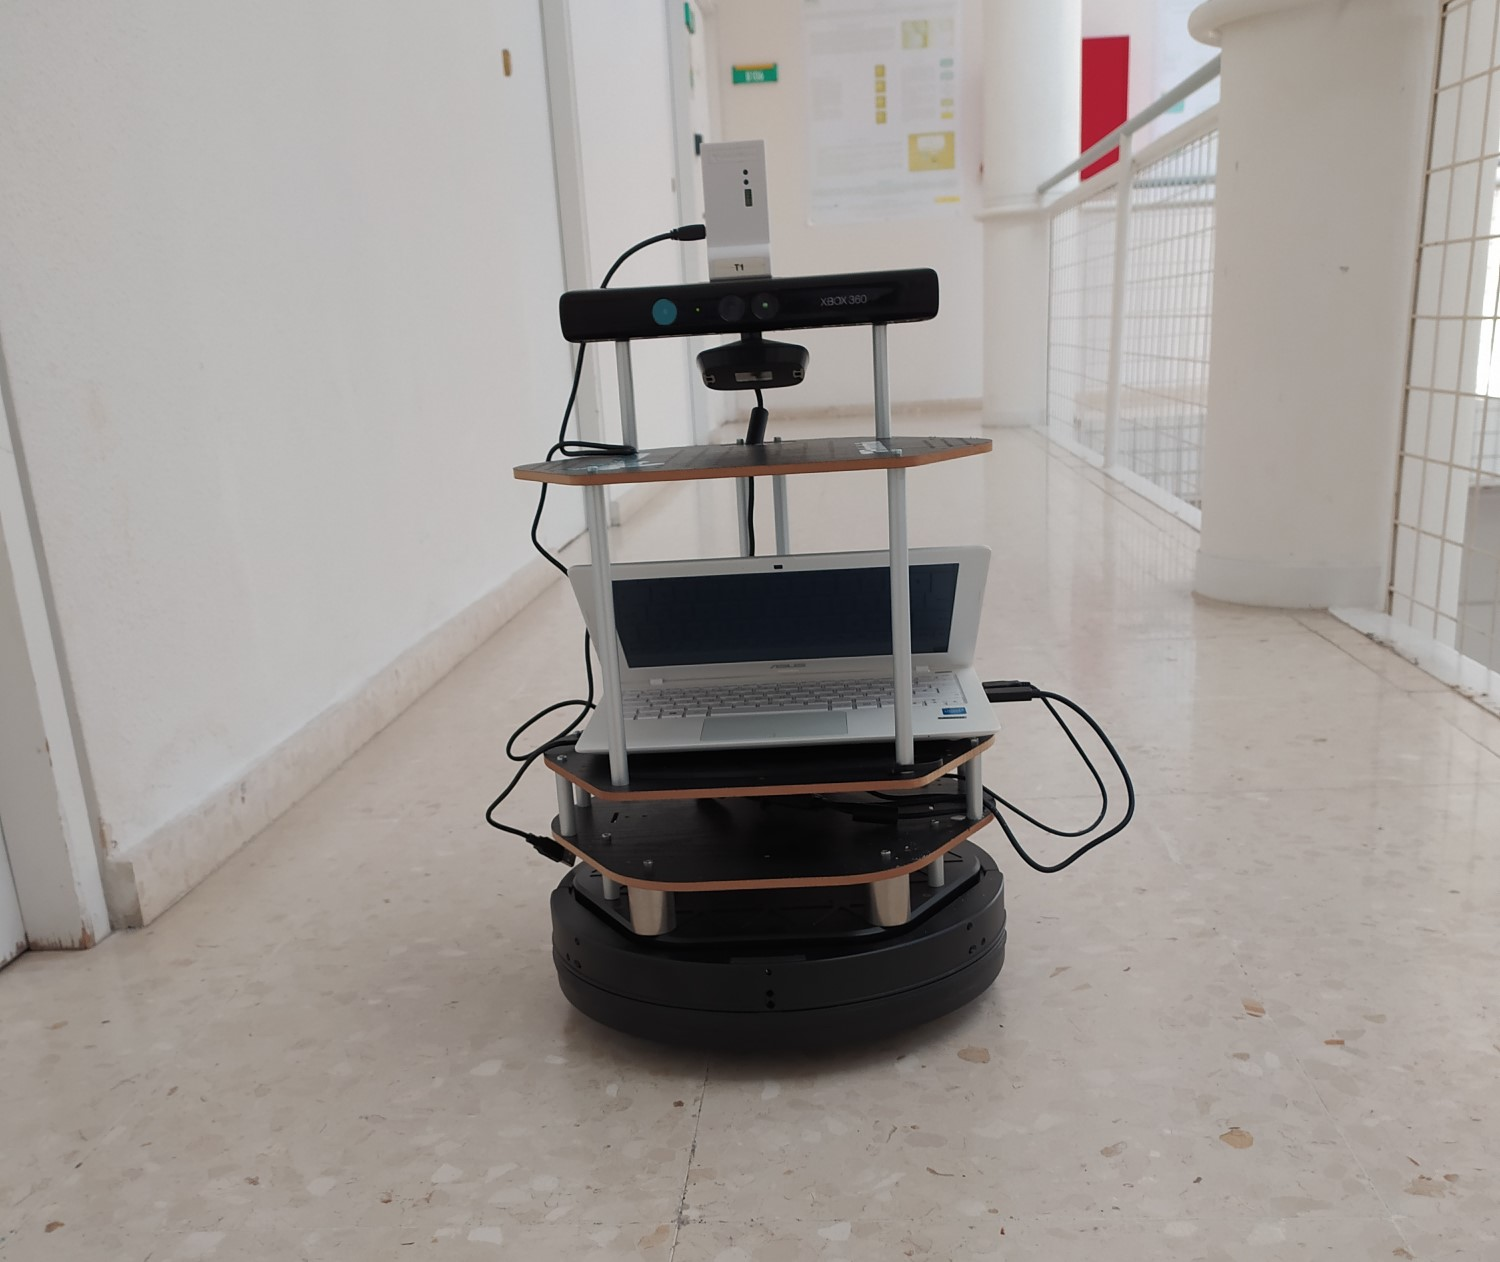
\includegraphics[width=0.75\textwidth]{pic/robot_fisica.jpg}
    \caption{Turtlebot en una de las tomas de medidas.}
    \label{fig:robot}
\end{figure}

El TurtleBot funciona con ROS --\textit{Robot Operating System}, en inglés--, un entorno de trabajo enfocado a los sistemas robóticos encargado del soporte para todos los dispositivos hardware del robot como motores, encoders o cámaras. 
Cuenta con diversas librerías para distintos casos de uso, entre las que se encuentra la navegación en un entorno controlado como la que se da en el caso de este trabajo.

Su funcionamiento se basa en una arquitectura de grafos, donde se definen \textit{nodos}, tareas en las que se realiza el procesamiento de sensores, control, actuadores o cualquier otra función.
Los nodos se comunican entre ellos con mensajes llamados \textit{topic}, y es posible su desarrollo con los lenguajes C++ y Python.

Dentro de los paquetes disponibles, el usado en el desarrollo del trabajo es el encargado de la navegación del robot, que permite desplazar al robot a cualquier punto del entorno de trabajo y proporcionar de forma constante su posición en el mapa.

Es posible acoplar al robot un sistema de visión llamado Kinect que, mediante luz, permite obtener un mapa de profundidad del entorno que lo rodea.
Fue desarrollado en primera instancia para el uso en videojuegos pero su uso también se ha extendido a labores de investigación al permitir el posicionamiento de objetos y paredes, de tal manera que permite al robot evitar obstáculos dinámicos en el caso de que interpongan en su camino.

La funcionalidad de navegación aprovecha estos sensores realizando una fusión de sus resultados con los datos de movimiento de los motores que impulsan al robot, de tal forma que es posible corregir cualquier error en casos donde el empuje de las ruedas no se traslade directamente en un desplazamiento del robot, como puede ocurrir al rotar sobre sí mismo.

Para conseguir el posicionamiento en el mapa el paquete de navegación utiliza un \textit{planner} global sobre el que es posible determinar las rutas a seguir por el robot para llegar a un punto dado sorteando obstáculos y paredes.
Junto a él trabaja un \textit{planner} local, en el que gracias a los sensores incorporados se evalúan de forma continua los alrededores del robot.
Así, es posible conseguir de forma continua una evaluación de los posibles obstáculos que no se encuentran en el mapa del planner global, para lo que se construye un mapa de costes con el fin de abortar el movimiento en el caso de que sea imposible alcanzar el punto objetivo \cite{ROSDoc}.

Con la información actualizada del \textit{planner} local, el \textit{planner} global es capaz de modificar los trayectos para que el robot pueda continuar su desplazamiento por el mapa.
Es posible observar un esquema del funcionamiento de estos sistemas en la Figura~\ref{fig:move_base}.

\begin{figure}[H]
    \centering
    \def\svgwidth{0.8\linewidth}
    \input{./fig/navigation.pdf_tex}
	\caption{Esquema del funcionamiento del paquete de navegación de ROS.}
    \label{fig:move_base}
\end{figure}

Con esta herramienta la librería de navegación permite un mapeado autónomo tomando como referencia los datos de odometría que proporcionan los motores propulsores del robot para determinar las dimensiones del entorno.

En el caso de disponer de antemano de dichas dimensiones es posible proporcionar un mapa al sistema de navegación y evitar el paso de reconocimiento del entorno.
Esto no solo ahorra tiempo, sino que además minimiza las posibles discrepancias entre los datos de odometría y los desplazamientos reales del robot al realizar el mapeado de forma autónoma.

La opción de realizar un mapa previo fue la elegida en este caso, ya que el robot cuenta con rutinas para el reposicionamiento en el mapa en dicho caso.
Así, a partir de los límites establecidos y comprobados de forma manual, las posibles discrepancias en la odometría del robot se ven continuamente compensadas y corregidas.

A partir de estos datos corregidos es posible conocer en cualquier momento la posición del robot en el mapa, expuesta a través de ROS en uno de los topic disponibles.

Para facilitar el uso de ROS existe la posibilidad de usar el simulador Stage, capaz de crear un mundo virtual a partir de un mapa en dos dimensiones en el que colocar el Turtlebot y simular su funcionamiento de forma total sin tener acceso al robot de forma física.
Es posible observar su interfaz en la Figura~\ref{fig:stage_rviz}.

Además, ROS también permite el uso de una herramienta de visualización de la posición del robot en el mapa y de todos los sensores que incorpora llamada \textit{rviz}.
Aunque es compatible con Stage, sus funcionalidades brillan al usar el robot en entornos reales, donde es posible comprobar de forma continua que su posicionamiento es correcto y que sus sensores funcionan como es debido.

\begin{figure}[H]
    \centering
    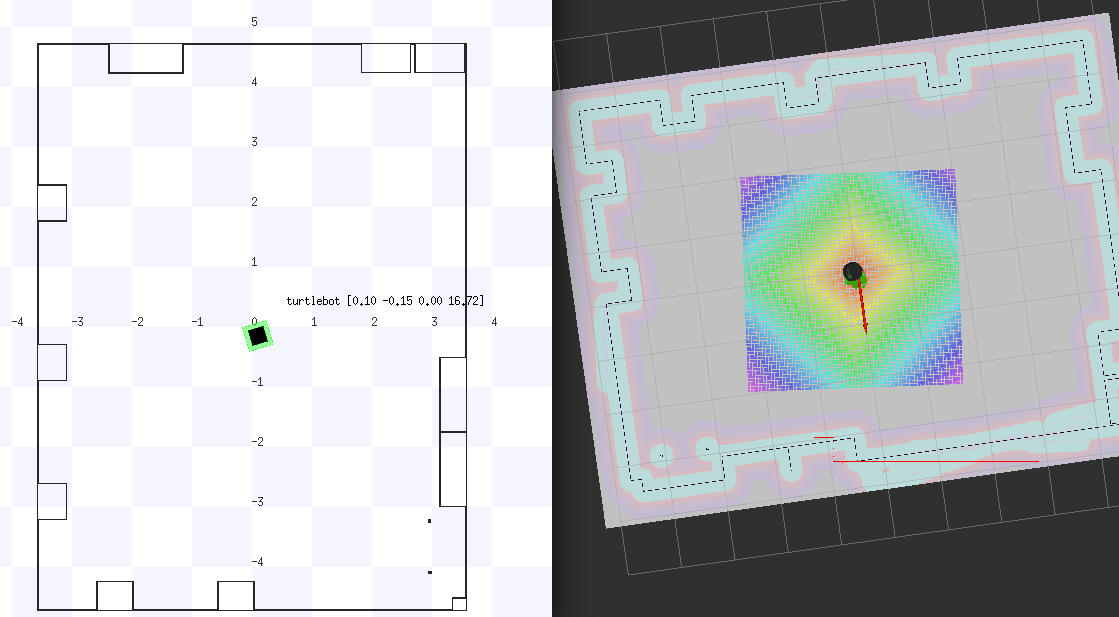
\includegraphics[width=0.75\textwidth]{pic/Stage-rviz.png}
    \caption{Captura del simulador Stage (a la izquierda) y la herramienta de visualización \textit{rviz} (a la derecha).}
    \label{fig:stage_rviz}
\end{figure}

\subsection{Sensores UWB}

Aunque el uso de UWB para el posicionamiento no está, al escribir este trabajo, utilizado de forma masiva, existen varias implementaciones comerciales de las técnicas geométricas mencionadas en secciones anteriores.
A pesar de que el uso de sensores propios es habitual, la adaptación de teléfonos móviles para la estimación de la posición también ha sido explorada por empresas como BeSpoon, a la espera de una implantación mayoritaria de hardware compatible en el diseño de estos dispositivos.

Los sensores utilizados han sido los pertenecientes al kit MDEK1001 ofertado por la empresa DecaWave.
Se trata de un sistema que ofrece, con una configuración mínima, la posibilidad de usar cualquiera de los componentes como baliza u objetivo.
Además, implementa un algoritmo de posicionamiento con al menos tres balizas de, según el fabricante, hasta 10~cm de precisión con visión directa \cite{Decawave}.

Este kit está formado por los módulos de desarrollo DW1001, encapsulados en una carcasa de plástico que permite colocarlos encima de una superficie plana o su colocación en paredes, como se puede observar en la Figura~\ref{fig:sensor_UWB}.
Permiten su uso con baterías, como fue el uso en este trabajo para las balizas, o a partir de alimentación a través del puerto USB utilizado para la recolección de datos.

\begin{figure}[H]
    \centering
    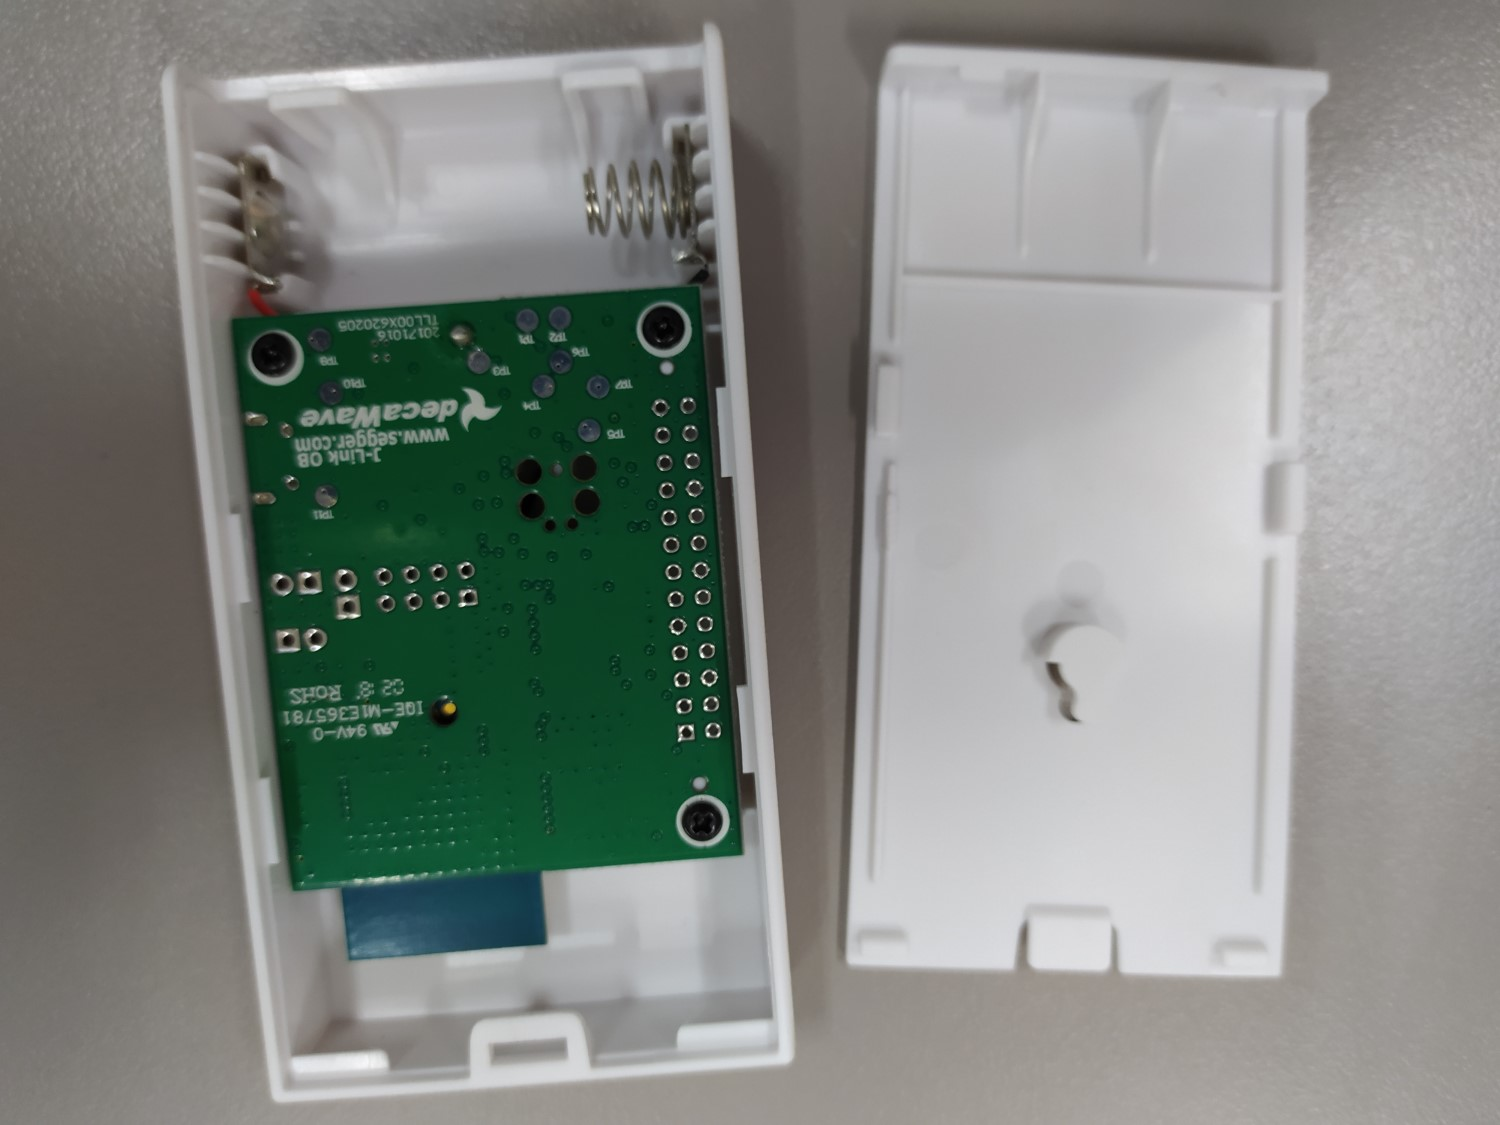
\includegraphics[width=0.65\textwidth]{pic/sensor_abierto.jpg}
    \caption{Módulo de sensor UWB DWM1001 dentro de la carcasa que lo contiene.}
    \label{fig:sensor_UWB}
\end{figure}

Algunas alternativas comerciales cuentan con antenas direccionales que permiten usar técnicas de AOA, pero no es el caso del kit utilizado que solo permite el posicionamiento con TOA y TDOA.

Los sensores, además de la comunicación por UWB, también permiten el uso de Bluetooth para su configuración como objetivos o balizas y en este último caso, para establecer la posición en la que se encuentran.
También permite configurar estas posiciones de las balizas de forma automática, aunque requiere que todas se coloquen en el mismo plano y en general una configuración manual proporcionará unos mejores resultados.

Para la comunicación por UWB los sensores utilizan el canal 5, con frecuencia central de $6.5$ GHz y ancho de banda de $499.2$ MHz que le permiten una tasa de datos de $6.81$ Mbps \cite{Decawave}.

El inicio de comercialización de dicho kit se remonta a 2017, por lo que no existe una amplia bibliografía sobre su uso en entornos reales más allá de los datos proporcionados por el fabricante.

En trabajos anteriores es posible encontrar mediciones tanto en entornos sin obstáculos con distancias bajas, en las que la precisión se encuentra en torno a los 18~cm \cite{Simedroni}; como en escenarios con distancias amplias y ciertas situaciones sin línea de visión directa, donde la discrepancias crecen hasta unos 50~cm \cite{jimenez, kulmer}.

DecaWave ofrece para su configuración y uso una aplicación para teléfonos móviles Android en la que representa en un mapa la posición de los sensores marcados como objetivos, pero también es posible una conexión a un ordenador como puerto serie.

Esta última opción permite obtener cuáles de las cuatro balizas --en el caso de que se configuren un número mayor de ellas-- se están usando en cada momento para realizar la estimación de la posición junto con la distancia calculada entre el objetivo y cada una de dichas balizas.

Además de la posición estimada, el algoritmo de posicionamiento proporciona un número entre 0 y 100 llamado «factor de calidad».
Debido a la naturaleza propietaria de este algoritmo, DecaWave no publica detalles sobre la obtención de este dato más allá de ser una comparación entre el posicionamiento obtenido con tres de las balizas y el obtenido al introducir la cuarta.


%------------------------------------------------------------------------------
%                             Metodologia
%------------------------------------------------------------------------------

\newpage
\section{Metodología}

Para la toma de datos se consideraron dos escenarios: el primero fue uno de los laboratorios situados en los Institutos Universitarios de Investigación de la Universidad de Extremadura, en el que se disponía de una superficie amplia y libre de objetos para tomar medidas en un escenario lo más cercano a lo ideal.

El segundo escenario fue la segunda planta del edificio B de la facultad de Física de la Universidad de Extremadura, elegido para acercarse a una disposición más general, con obstáculos entre las balizas y el objetivo.

\subsection{Toma de medidas}

En todos los casos la toma de medidas siguió el mismo procedimiento: en base a una trayectoria fijada que atraviesa una serie de puntos en cada escenario se toman un número prefijado de datos a partir de los sensores, con el robot parado en cada uno de dichos puntos.

Para determinar el número de medidas a tomar en cada caso se realizaron tomas de medidas previas para determinar la naturaleza de los datos obtenidos.
En todos los casos se obtuvo una distribución de tipo gaussiano, como se puede ver en la figura \ref{fig:datos_sensor}, por lo que se tomaron 50 datos en el caso del laboratorio y 250 en el caso del edificio de Física con el objetivo tener una dispersión al menos menor de 2cm tomando el mínimo número de datos.

\begin{figure}[H]
  \begin{subfigure}[b]{.5\textwidth}
    \centering
    \begin{tikzpicture}
\begin{axis}[width = \textwidth, height = 0.9\textwidth,ymin=0,xlabel={Posicion (cm)}]
    \addplot [hist={bins=10,data=x}, fill=black!50]
    table {data/ejemplo_sensores.txt};
    % table [x index=0, y index=1, z index=3] {data/ejemplo_sensores.txt};
\end{axis}
\end{tikzpicture} 
    \caption{Eje x}
    \label{fig:hist_x}
  \end{subfigure}
  \begin{subfigure}[b]{.5\textwidth}
    \centering
    \begin{tikzpicture}
\begin{axis}[width = \textwidth, height = 0.9\textwidth,ymin=0,xlabel={Posicion (cm)}]
    \addplot [hist={bins=10,data=y}, fill=black!50]
    table {data/ejemplo_sensores.txt};
    % table [x index=0, y index=1, z index=3] {data/ejemplo_sensores.txt};
\end{axis}
\end{tikzpicture}
    \caption{Eje y}
    \label{fig:hist_y}
  \end{subfigure}
  \caption{Histograma del posicionamiento de los sensores en uno de los puntos}
  \label{fig:datos_sensor}
\end{figure}

Además, para eliminar cualquier tipo de anomalía estadística cada trayectoria se repitió un mínimo de tres veces, tras las que se evaluaron los datos.
En los casos en los que la dispersión fue excesiva, se procedió a repetir de nuevo estas mediciones.

En las primeras tomas, donde se orientaba el robot hacia el siguiente punto de tal forma que su desplazamiento tomase el menor tiempo posible, se observó que el diseño de las antenas de los sensores utilizados, con una ganancia ligeramente dependiente del ángulo de incidencia \cite{ang}, hacía que, al girar el sensor asignado como objetivo, la estimación de su posición variase.

Esta observación también ha sido recogida en trabajos previos \cite{MSTesis}, donde se intentaba corregir a partir de medidas con distintos ángulos de incidencia.
Esto no es posible en el caso de este trabajo, ya que no versa sobre el desarrollo de un algoritmo de posicionamiento, sino sobre la precisión del ya implementado.
El algoritmo utilizado es propiedad de la empresa fabricante de los sensores, que no ha liberado detalles sobre su implementación, lo que hace imposible cualquier corrección.

Así, para minimizar este obstáculo todas las medidas que figuran en los resultados están tomadas colocando al robot con el mismo ángulo respecto a las balizas, de tal manera que no es necesario considerar variaciones en la posición obtenida debido a su orientación.

\subsection{Laboratorio}

La primera toma de medidas tuvo lugar en el laboratorio 0L3 de los Institutos Universitarios de Investigación, donde se disponía de una superficie de aproximadamente 5 metros por 7 metros completamente libre para usar por el robot.

Debido a la libertad a la hora de recorrer dicha superficie se eligieron tres trayectorias que cubriesen todos los puntos a evaluar, establecidos en una cuadrícula con una separación de 1 metro entre cada uno de ellos de tal forma que se evitase un posible sesgo en el movimiento del robot.

\begin{figure}[H]
    \begin{subfigure}[b]{.3\textwidth}
      \centering
      \def\svgwidth{0.8\linewidth}
	    \input{./fig/lab.pdf_tex} 
      \caption{Puntos a evaluar}
      \label{fig:puntos}
    \end{subfigure}
    \begin{subfigure}[b]{.3\textwidth}
      \centering
      \def\svgwidth{0.8\linewidth}
	    \input{./fig/lab_espiral.pdf_tex} 
      \caption{Trayectoria en espiral}
      \label{fig:espiral}
    \end{subfigure}
    \begin{subfigure}[b]{.3\textwidth}
        \centering
        \def\svgwidth{0.8\linewidth}
	    \input{./fig/lab_vertical.pdf_tex} 
        \caption{Trayectoria en vertical}
        \label{fig:vertical}
      \end{subfigure}
    \caption{Disposición del laboratorio}
    \label{fig:laboratorio}
\end{figure}

La primera de estas trayectorias tenía un recorrido con origen en el centro del laboratorio, acercándose a las paredes exteriores en forma de espiral, con algunas modificaciones para asegurar el paso por todos los puntos.

El segundo trayecto hacía que el robot avanzase de forma recta siguiendo líneas verticales --en el sentido tal y como se ha planteado la representación en dos dimensiones en la figura \ref{fig:vertical}--, con separación de un metro entre cada punto.

Por último se diseñó una trayectoria en la que robot pasase de forma aleatoria por los 35 puntos a medir, de tal forma que en cada intento el orden fuese distinto.

Para comprobar en este escenario ideal el efecto de la colocación de las balizas se repitió la toma de medida en dos configuraciones, colocando 4 y 6 sensores respectivamente.
Teniendo en cuenta que el sistema empleado solo utiliza cuatro de las balizas para el posicionamiento del objetivo, el uso de la configuraciones con 6 de los sensores solo afecta a la posición de dichas baliza en los cálculos, usando siempre los cuatro sensores más cercanos.

La altura a la que fueron colocadas los sensores que actúan como balizas se vio restringida por el mobiliario del laboratorio, de modo que la mayoría se encontraban a unos 180cm del suelo con una de ellas a 80cm y otra a 200cm, aunque el sistema de los sensores permite estas diferencias de alturas en el modo de configuración manual de las balizas.

\begin{figure}[H]
  \begin{subfigure}[b]{.5\textwidth}
    \centering
    \def\svgwidth{0.7\linewidth}
    \input{./fig/lab_4sensores.pdf_tex} 
    \caption{4 balizas}
    \label{fig:lab_4sens}
  \end{subfigure}
  \ \
  \begin{subfigure}[b]{.5\textwidth}
    \centering
    \def\svgwidth{0.82\linewidth}
    \input{./fig/lab_6sensores.pdf_tex}  
    \caption{6 balizas}
    \label{fig:lab_6sens}
  \end{subfigure}
  \caption{Configuraciones de las balizas en el laboratorio}
  \label{fig:lab_sensores}
\end{figure}

\subsection{Edificio de la facultad de Física}

En el segundo escenario aparecen elementos más cercanos a una implementación de un sistema de posicionamiento local habitual: obstáculos en las balizas, que no es posible colocar en cualquier lugar, y un tránsito de personas habitual que podía interferir en la señal del sistema utilizado.

En este caso todas las medidas fueron tomadas utilizando la misma trayectoria, que seguía los pasillos de la planta del edificio al no poder optar a más variaciones.

\begin{figure}[H]
  \begin{subfigure}[b]{.5\textwidth}
    \centering
    \def\svgwidth{0.75\linewidth}
    \input{./fig/fisica_num.pdf_tex} 
    \caption{Puntos a evaluar}
    \label{fig:puntos_fisica}
  \end{subfigure}
  \begin{subfigure}[b]{.5\textwidth}
    \centering
    \def\svgwidth{0.75\linewidth}
    \input{./fig/fisica_tray.pdf_tex} 
    \caption{Trayectoria}
    \label{fig:trayecto_fisica}
  \end{subfigure}
  \caption{Disposición de la planta del edificio de Física}
  \label{fig:fisica}
\end{figure}

Al igual que en el caso del laboratorio, se repitieron las medidas con distintas configuraciones de las balizas, con tres alternativas en este caso: 4, 6 y 8 balizas repartidas de la forma más uniforme posible.

\begin{figure}[H]
  \begin{subfigure}[b]{.3\textwidth}
    \centering
    \def\svgwidth{0.9\linewidth}
    \input{./fig/fisica_4sens.pdf_tex} 
    \caption{4 balizas}
    \label{fig:puntos}
  \end{subfigure}
  \begin{subfigure}[b]{.3\textwidth}
    \centering
    \def\svgwidth{0.9\linewidth}
    \input{./fig/fisica_6sens.pdf_tex}  
    \caption{6 balizas}
    \label{fig:espiral}
  \end{subfigure}
  \begin{subfigure}[b]{.3\textwidth}
      \centering
      \def\svgwidth{0.9\linewidth}
      \input{./fig/fisica_8sens.pdf_tex}  
      \caption{8 balizas}
      \label{fig:vertical}
    \end{subfigure}
  \caption{Configuraciones de las balizas en el edificio de Física}
  \label{fig:sensores_fisica}
\end{figure}

Como en el caso del laboratorio, el kit de sensores UWB utilizado solo usa 4 de las balizas disponibles para estimar la posición del objetivo, por lo que el número mayor de sensores colocados permite una mayor libertad al elegir las balizas con mejor recepción de la señal pero no afinar la estimación con un número mayor de muestras para determinar la intersección de las curvas que definen.

Como es posible ver en la figura \ref{fig:sensores_fisica} la posición de los sensores no es completamente uniforme, debido a que no toda la superficie de la planta estaba disponible por la disposición de los despachos y laboratorios.
En este caso la altura de todas las balizas fue similar, en torno a los 170cm respecto al suelo.

%------------------------------------------------------------------------------
%                             Resultados
%------------------------------------------------------------------------------

\newpage
\section{Resultados}

Tal y como viene recogido en las sección anterior, en la toma de medidas se recabaron datos desde dos fuentes: el posicionamiento local del robot y los cálculos del kit de sensores de UWB.

Para el análisis de los resultados se han considerado a los datos obtenidos por el posicionamiento local del robot como \textit{ground truth}, es decir, como la posición verdadera del sensor establecido como objetivo, que está colocado encima del robot.
A partir de esta consideración, es posible definir el error en la posición para cada uno de los ejes cartesianos como
\begin{equation}\label{eq:Diff_eje}
    \text{Error eje} = \text{Valor posición robot} - \text{Valor posición sensores}
\end{equation}

El kit utilizado permite el posicionamiento en tres dimensiones, aunque no se presentarán y estudiarán los resultados en el eje vertical, ya que el sensor a posicionar se encontraba en todo momento encima del robot, a la misma altura.

Además de las diferencias en cada eje se evaluará la discrepancia en la posición, a partir del vector definido como la diferencia de los vectores de posición del robot y los sensores como se indica en la Figura~\ref{fig:diff_pos}.
\begin{figure}[H]
    \centering
    \begin{tikzpicture}
    % Ejes
    \draw [->, thick] (0,0) -- (7,0);
    \draw [->, thick] (0,0) -- (0,3);

    % Vectores

    \draw [->, ultra thick] (0,0) -- (5,1);
    \draw [->, ultra thick] (0,0) -- (2.5,2);
    \draw [->, red, ultra thick] (2.5,2) -- (5,1);

    \node[rotate=-20, red] at (3.7,1.9) {$\Delta$ Pos};
    \node[rotate=12] at (2.7,0.9) {Pos. sensor};
    \node[rotate=40] at (1.1,1.3) {Pos. robot};

\end{tikzpicture}
    \caption{Definición del vector de error de posición.}
    \label{fig:diff_pos}
\end{figure}

Así, las componentes de dicho vector son las definidas en \eqref{eq:Diff_eje} y su módulo, que será interpretado como el error en posición se define como

\begin{equation}\label{eq:vec_pos}
    \text{Error en posición} = \sqrt{(\text{Error } x)^2 + (\text{Error } y)^2}
\end{equation}

A la hora de interpretar los resultados a partir de la toma de medidas y con el tratamiento especificado cabe recordar que en \eqref{eq:Diff_eje} se incluyen dos fuentes de error, por un lado el posicionamiento local del robot y por otro el posicionamiento por triliteración de los sensores de UWB.

La evaluación de la bondad del posicionamiento de los sensores, teniendo en cuenta la posibilidad de tomar con ellos tantas medidas como sea posible, es directa, dando en todos los casos una distribución gaussiana, como era de esperar y como se podía ver en la Figura~\ref{fig:datos_sensor}; aun así, según los datos proporcionados por el fabricante y contrastados en trabajos previos nos da unos errores de como mínimo 10~cm.

En el caso del robot los sistemas de posicionamiento local propios, basados en la fusión de datos de odometría y de posicionamiento de objetos del entorno arrojan un error en la posición de 10~cm, con un perfil también normal \cite{POSRobot}.
% PREGUNTAR ESTO. Como poner cada eje?
% Sin embargo, dependen también de la presencia de paredes u objetos contra los que comparar los datos de odometría que proporcionan los motores lo mueven.

La adición de ambas fuentes de error --robot y sensores--, siguiendo el teorema del límite central, nos dará una distribución que tenderá con un número creciente de medias hacia otra distribución gaussiana con el error total en la posición.
Teniendo en cuenta que los errores de posicionamiento no son absolutos, será posible encontrar casos puntuales en los que la adición de ambas fuentes de error proporcione un error total con un valor menor que cada uno de los errores por separado, compensándose entre sí.

La toma de numerosas medidas con distintas rutas trata de minimizar este hecho, de tal forma que, de media, es razonable esperar un error en el posicionamiento en torno a los 20~cm, en el caso de \eqref{eq:vec_pos}.

\subsection{Laboratorio de Robótica del ICCAEx}

Como se comentaba en la sección de metodología, se diseñaron varias trayectorias a recorrer por el robot para así eliminar cualquier sesgo en los errores de su posicionamiento local.

Los resultados expuestos en esta sección son fruto de la composición de las medidas de todas las trayectorias recorridas por el robot en cada caso.
En el Apéndice A es posible encontrar tablas con los datos de cada trayectoria por separado.

\subsubsection{4 balizas}

Con la configuración de cuatro balizas definida en la Figura~\ref{fig:lab_4sens} se obtuvieron los datos recopilados en las Tablas \ref{tab:media_lab_4_vertical} para la trayectoria vertical, \ref{tab:media_lab_4_espiral} para la trayectoria en espiral y \ref{tab:media_lab_4_aleatoria} para la trayectoria aleatoria.

Los datos acumulados de las tres trayectorias están recogidos en la Tabla \ref{tab:media_lab_4_total}, y representados en Figura~\ref{fig:res_lab}.
% \footnote{La presentación de los resultados expuestos a lo largo de la sección se han obtenido por interpolación a partir de las referencias definidas por los valores experimentales los puntos medidos, separados por un metro en el caso del laboratorio e indicados con el valor obtenido en cada cada uno de ellos sobre el lugar donde se obtuvo. La interpolación fue realizada usando splines bicúbicos, de tal manera que los valores en los puntos de referencia no han sido alterados.
% Entre paréntesis se indica la desviación estándar de los valores obtenidos en cada punto.}
Es posible observar un valor muy alto en la discrepancia en en el eje $x$ en el punto 34 --definido en la Figura~\ref{fig:puntos}--.
Teniendo en cuenta que en los puntos adyacentes no ocurre, es posible achacar esta alta discrepancia a puras fluctuaciones estadísticas o, de forma más probable, a una falta de visión directa entre objetivo y balizas, teniendo en cuenta que no se repite en más puntos.

Para tratar de comprobar el comportamiento general de la combinación de sensores y robot más allá de puntos con valores especialmente altos o bajos se recoge la Tabla~\ref{tab:resumen_lab_4} con los valores medios y dispersión del error a lo largo de cada uno de los ejes y del error en el posicionamiento en el caso de uso de 4 balizas.

\begin{figure}[H]
    \centering
    \hspace*{-0.5cm}
    %% Creator: Matplotlib, PGF backend
%%
%% To include the figure in your LaTeX document, write
%%   \input{<filename>.pgf}
%%
%% Make sure the required packages are loaded in your preamble
%%   \usepackage{pgf}
%%
%% and, on pdftex
%%   \usepackage[utf8]{inputenc}\DeclareUnicodeCharacter{2212}{-}
%%
%% or, on luatex and xetex
%%   \usepackage{unicode-math}
%%
%% Figures using additional raster images can only be included by \input if
%% they are in the same directory as the main LaTeX file. For loading figures
%% from other directories you can use the `import` package
%%   \usepackage{import}
%%
%% and then include the figures with
%%   \import{<path to file>}{<filename>.pgf}
%%
%% Matplotlib used the following preamble
%%   \usepackage[utf8x]{inputenc}
%%   \usepackage[T1]{fontenc}
%%
\begingroup%
\makeatletter%
\begin{pgfpicture}%
\pgfpathrectangle{\pgfpointorigin}{\pgfqpoint{7.000000in}{5.000000in}}%
\pgfusepath{use as bounding box, clip}%
\begin{pgfscope}%
\pgfsetbuttcap%
\pgfsetmiterjoin%
\definecolor{currentfill}{rgb}{1.000000,1.000000,1.000000}%
\pgfsetfillcolor{currentfill}%
\pgfsetlinewidth{0.000000pt}%
\definecolor{currentstroke}{rgb}{1.000000,1.000000,1.000000}%
\pgfsetstrokecolor{currentstroke}%
\pgfsetdash{}{0pt}%
\pgfpathmoveto{\pgfqpoint{0.000000in}{0.000000in}}%
\pgfpathlineto{\pgfqpoint{7.000000in}{0.000000in}}%
\pgfpathlineto{\pgfqpoint{7.000000in}{5.000000in}}%
\pgfpathlineto{\pgfqpoint{0.000000in}{5.000000in}}%
\pgfpathclose%
\pgfusepath{fill}%
\end{pgfscope}%
\begin{pgfscope}%
\pgfsetbuttcap%
\pgfsetmiterjoin%
\definecolor{currentfill}{rgb}{1.000000,1.000000,1.000000}%
\pgfsetfillcolor{currentfill}%
\pgfsetlinewidth{0.000000pt}%
\definecolor{currentstroke}{rgb}{0.000000,0.000000,0.000000}%
\pgfsetstrokecolor{currentstroke}%
\pgfsetstrokeopacity{0.000000}%
\pgfsetdash{}{0pt}%
\pgfpathmoveto{\pgfqpoint{0.875000in}{2.728322in}}%
\pgfpathlineto{\pgfqpoint{2.013112in}{2.728322in}}%
\pgfpathlineto{\pgfqpoint{2.013112in}{4.321678in}}%
\pgfpathlineto{\pgfqpoint{0.875000in}{4.321678in}}%
\pgfpathclose%
\pgfusepath{fill}%
\end{pgfscope}%
\begin{pgfscope}%
\pgfpathrectangle{\pgfqpoint{0.875000in}{2.728322in}}{\pgfqpoint{1.138112in}{1.593357in}}%
\pgfusepath{clip}%
\pgfsys@transformshift{0.875000in}{2.728322in}%
\pgftext[left,bottom]{
\includegraphics[interpolate=true,width=1.140000in,height=1.600000in]{graph/res/4sensores-img0.png}}%
\end{pgfscope}%
\begin{pgfscope}%
\pgfsetrectcap%
\pgfsetmiterjoin%
\pgfsetlinewidth{0.803000pt}%
\definecolor{currentstroke}{rgb}{0.000000,0.000000,0.000000}%
\pgfsetstrokecolor{currentstroke}%
\pgfsetdash{}{0pt}%
\pgfpathmoveto{\pgfqpoint{0.875000in}{2.728322in}}%
\pgfpathlineto{\pgfqpoint{0.875000in}{4.321678in}}%
\pgfusepath{stroke}%
\end{pgfscope}%
\begin{pgfscope}%
\pgfsetrectcap%
\pgfsetmiterjoin%
\pgfsetlinewidth{0.803000pt}%
\definecolor{currentstroke}{rgb}{0.000000,0.000000,0.000000}%
\pgfsetstrokecolor{currentstroke}%
\pgfsetdash{}{0pt}%
\pgfpathmoveto{\pgfqpoint{2.013112in}{2.728322in}}%
\pgfpathlineto{\pgfqpoint{2.013112in}{4.321678in}}%
\pgfusepath{stroke}%
\end{pgfscope}%
\begin{pgfscope}%
\pgfsetrectcap%
\pgfsetmiterjoin%
\pgfsetlinewidth{0.803000pt}%
\definecolor{currentstroke}{rgb}{0.000000,0.000000,0.000000}%
\pgfsetstrokecolor{currentstroke}%
\pgfsetdash{}{0pt}%
\pgfpathmoveto{\pgfqpoint{0.875000in}{2.728322in}}%
\pgfpathlineto{\pgfqpoint{2.013112in}{2.728322in}}%
\pgfusepath{stroke}%
\end{pgfscope}%
\begin{pgfscope}%
\pgfsetrectcap%
\pgfsetmiterjoin%
\pgfsetlinewidth{0.803000pt}%
\definecolor{currentstroke}{rgb}{0.000000,0.000000,0.000000}%
\pgfsetstrokecolor{currentstroke}%
\pgfsetdash{}{0pt}%
\pgfpathmoveto{\pgfqpoint{0.875000in}{4.321678in}}%
\pgfpathlineto{\pgfqpoint{2.013112in}{4.321678in}}%
\pgfusepath{stroke}%
\end{pgfscope}%
\begin{pgfscope}%
\definecolor{textcolor}{rgb}{0.000000,0.000000,0.000000}%
\pgfsetstrokecolor{textcolor}%
\pgfsetfillcolor{textcolor}%
\pgftext[x=1.444056in,y=4.405012in,,base]{\color{textcolor}\rmfamily\fontsize{12.000000}{14.400000}\selectfont Eje x}%
\end{pgfscope}%
\begin{pgfscope}%
\pgfsetbuttcap%
\pgfsetmiterjoin%
\definecolor{currentfill}{rgb}{1.000000,1.000000,1.000000}%
\pgfsetfillcolor{currentfill}%
\pgfsetlinewidth{0.000000pt}%
\definecolor{currentstroke}{rgb}{0.000000,0.000000,0.000000}%
\pgfsetstrokecolor{currentstroke}%
\pgfsetstrokeopacity{0.000000}%
\pgfsetdash{}{0pt}%
\pgfpathmoveto{\pgfqpoint{0.875000in}{0.628322in}}%
\pgfpathlineto{\pgfqpoint{2.013112in}{0.628322in}}%
\pgfpathlineto{\pgfqpoint{2.013112in}{2.221678in}}%
\pgfpathlineto{\pgfqpoint{0.875000in}{2.221678in}}%
\pgfpathclose%
\pgfusepath{fill}%
\end{pgfscope}%
\begin{pgfscope}%
\pgfpathrectangle{\pgfqpoint{0.875000in}{0.628322in}}{\pgfqpoint{1.138112in}{1.593357in}}%
\pgfusepath{clip}%
\pgfsys@transformshift{0.875000in}{0.628322in}%
\pgftext[left,bottom]{
\includegraphics[interpolate=true,width=1.140000in,height=1.600000in]{graph/res/4sensores-img1.png}}%
\end{pgfscope}%
\begin{pgfscope}%
\pgfsetrectcap%
\pgfsetmiterjoin%
\pgfsetlinewidth{0.803000pt}%
\definecolor{currentstroke}{rgb}{0.000000,0.000000,0.000000}%
\pgfsetstrokecolor{currentstroke}%
\pgfsetdash{}{0pt}%
\pgfpathmoveto{\pgfqpoint{0.875000in}{0.628322in}}%
\pgfpathlineto{\pgfqpoint{0.875000in}{2.221678in}}%
\pgfusepath{stroke}%
\end{pgfscope}%
\begin{pgfscope}%
\pgfsetrectcap%
\pgfsetmiterjoin%
\pgfsetlinewidth{0.803000pt}%
\definecolor{currentstroke}{rgb}{0.000000,0.000000,0.000000}%
\pgfsetstrokecolor{currentstroke}%
\pgfsetdash{}{0pt}%
\pgfpathmoveto{\pgfqpoint{2.013112in}{0.628322in}}%
\pgfpathlineto{\pgfqpoint{2.013112in}{2.221678in}}%
\pgfusepath{stroke}%
\end{pgfscope}%
\begin{pgfscope}%
\pgfsetrectcap%
\pgfsetmiterjoin%
\pgfsetlinewidth{0.803000pt}%
\definecolor{currentstroke}{rgb}{0.000000,0.000000,0.000000}%
\pgfsetstrokecolor{currentstroke}%
\pgfsetdash{}{0pt}%
\pgfpathmoveto{\pgfqpoint{0.875000in}{0.628322in}}%
\pgfpathlineto{\pgfqpoint{2.013112in}{0.628322in}}%
\pgfusepath{stroke}%
\end{pgfscope}%
\begin{pgfscope}%
\pgfsetrectcap%
\pgfsetmiterjoin%
\pgfsetlinewidth{0.803000pt}%
\definecolor{currentstroke}{rgb}{0.000000,0.000000,0.000000}%
\pgfsetstrokecolor{currentstroke}%
\pgfsetdash{}{0pt}%
\pgfpathmoveto{\pgfqpoint{0.875000in}{2.221678in}}%
\pgfpathlineto{\pgfqpoint{2.013112in}{2.221678in}}%
\pgfusepath{stroke}%
\end{pgfscope}%
\begin{pgfscope}%
\definecolor{textcolor}{rgb}{0.000000,0.000000,0.000000}%
\pgfsetstrokecolor{textcolor}%
\pgfsetfillcolor{textcolor}%
\pgftext[x=1.444056in,y=2.305012in,,base]{\color{textcolor}\rmfamily\fontsize{12.000000}{14.400000}\selectfont Eje y}%
\end{pgfscope}%
\begin{pgfscope}%
\pgfsetbuttcap%
\pgfsetmiterjoin%
\definecolor{currentfill}{rgb}{1.000000,1.000000,1.000000}%
\pgfsetfillcolor{currentfill}%
\pgfsetlinewidth{0.000000pt}%
\definecolor{currentstroke}{rgb}{0.000000,0.000000,0.000000}%
\pgfsetstrokecolor{currentstroke}%
\pgfsetstrokeopacity{0.000000}%
\pgfsetdash{}{0pt}%
\pgfpathmoveto{\pgfqpoint{2.791259in}{0.550000in}}%
\pgfpathlineto{\pgfqpoint{5.541259in}{0.550000in}}%
\pgfpathlineto{\pgfqpoint{5.541259in}{4.400000in}}%
\pgfpathlineto{\pgfqpoint{2.791259in}{4.400000in}}%
\pgfpathclose%
\pgfusepath{fill}%
\end{pgfscope}%
\begin{pgfscope}%
\pgfpathrectangle{\pgfqpoint{2.791259in}{0.550000in}}{\pgfqpoint{2.750000in}{3.850000in}}%
\pgfusepath{clip}%
\pgfsys@transformshift{2.791259in}{0.550000in}%
\pgftext[left,bottom]{
\includegraphics[interpolate=true,width=2.750000in,height=3.850000in]{graph/res/4sensores-img2.png}}%
\end{pgfscope}%
\begin{pgfscope}%
\pgfsetbuttcap%
\pgfsetroundjoin%
\definecolor{currentfill}{rgb}{0.000000,0.000000,0.000000}%
\pgfsetfillcolor{currentfill}%
\pgfsetlinewidth{0.803000pt}%
\definecolor{currentstroke}{rgb}{0.000000,0.000000,0.000000}%
\pgfsetstrokecolor{currentstroke}%
\pgfsetdash{}{0pt}%
\pgfsys@defobject{currentmarker}{\pgfqpoint{0.000000in}{-0.048611in}}{\pgfqpoint{0.000000in}{0.000000in}}{%
\pgfpathmoveto{\pgfqpoint{0.000000in}{0.000000in}}%
\pgfpathlineto{\pgfqpoint{0.000000in}{-0.048611in}}%
\pgfusepath{stroke,fill}%
}%
\begin{pgfscope}%
\pgfsys@transformshift{3.066259in}{0.550000in}%
\pgfsys@useobject{currentmarker}{}%
\end{pgfscope}%
\end{pgfscope}%
\begin{pgfscope}%
\definecolor{textcolor}{rgb}{0.000000,0.000000,0.000000}%
\pgfsetstrokecolor{textcolor}%
\pgfsetfillcolor{textcolor}%
\pgftext[x=3.066259in,y=0.452778in,,top]{\color{textcolor}\rmfamily\fontsize{10.000000}{12.000000}\selectfont -2}%
\end{pgfscope}%
\begin{pgfscope}%
\pgfsetbuttcap%
\pgfsetroundjoin%
\definecolor{currentfill}{rgb}{0.000000,0.000000,0.000000}%
\pgfsetfillcolor{currentfill}%
\pgfsetlinewidth{0.803000pt}%
\definecolor{currentstroke}{rgb}{0.000000,0.000000,0.000000}%
\pgfsetstrokecolor{currentstroke}%
\pgfsetdash{}{0pt}%
\pgfsys@defobject{currentmarker}{\pgfqpoint{0.000000in}{-0.048611in}}{\pgfqpoint{0.000000in}{0.000000in}}{%
\pgfpathmoveto{\pgfqpoint{0.000000in}{0.000000in}}%
\pgfpathlineto{\pgfqpoint{0.000000in}{-0.048611in}}%
\pgfusepath{stroke,fill}%
}%
\begin{pgfscope}%
\pgfsys@transformshift{3.616259in}{0.550000in}%
\pgfsys@useobject{currentmarker}{}%
\end{pgfscope}%
\end{pgfscope}%
\begin{pgfscope}%
\definecolor{textcolor}{rgb}{0.000000,0.000000,0.000000}%
\pgfsetstrokecolor{textcolor}%
\pgfsetfillcolor{textcolor}%
\pgftext[x=3.616259in,y=0.452778in,,top]{\color{textcolor}\rmfamily\fontsize{10.000000}{12.000000}\selectfont -1}%
\end{pgfscope}%
\begin{pgfscope}%
\pgfsetbuttcap%
\pgfsetroundjoin%
\definecolor{currentfill}{rgb}{0.000000,0.000000,0.000000}%
\pgfsetfillcolor{currentfill}%
\pgfsetlinewidth{0.803000pt}%
\definecolor{currentstroke}{rgb}{0.000000,0.000000,0.000000}%
\pgfsetstrokecolor{currentstroke}%
\pgfsetdash{}{0pt}%
\pgfsys@defobject{currentmarker}{\pgfqpoint{0.000000in}{-0.048611in}}{\pgfqpoint{0.000000in}{0.000000in}}{%
\pgfpathmoveto{\pgfqpoint{0.000000in}{0.000000in}}%
\pgfpathlineto{\pgfqpoint{0.000000in}{-0.048611in}}%
\pgfusepath{stroke,fill}%
}%
\begin{pgfscope}%
\pgfsys@transformshift{4.166259in}{0.550000in}%
\pgfsys@useobject{currentmarker}{}%
\end{pgfscope}%
\end{pgfscope}%
\begin{pgfscope}%
\definecolor{textcolor}{rgb}{0.000000,0.000000,0.000000}%
\pgfsetstrokecolor{textcolor}%
\pgfsetfillcolor{textcolor}%
\pgftext[x=4.166259in,y=0.452778in,,top]{\color{textcolor}\rmfamily\fontsize{10.000000}{12.000000}\selectfont 0}%
\end{pgfscope}%
\begin{pgfscope}%
\pgfsetbuttcap%
\pgfsetroundjoin%
\definecolor{currentfill}{rgb}{0.000000,0.000000,0.000000}%
\pgfsetfillcolor{currentfill}%
\pgfsetlinewidth{0.803000pt}%
\definecolor{currentstroke}{rgb}{0.000000,0.000000,0.000000}%
\pgfsetstrokecolor{currentstroke}%
\pgfsetdash{}{0pt}%
\pgfsys@defobject{currentmarker}{\pgfqpoint{0.000000in}{-0.048611in}}{\pgfqpoint{0.000000in}{0.000000in}}{%
\pgfpathmoveto{\pgfqpoint{0.000000in}{0.000000in}}%
\pgfpathlineto{\pgfqpoint{0.000000in}{-0.048611in}}%
\pgfusepath{stroke,fill}%
}%
\begin{pgfscope}%
\pgfsys@transformshift{4.716259in}{0.550000in}%
\pgfsys@useobject{currentmarker}{}%
\end{pgfscope}%
\end{pgfscope}%
\begin{pgfscope}%
\definecolor{textcolor}{rgb}{0.000000,0.000000,0.000000}%
\pgfsetstrokecolor{textcolor}%
\pgfsetfillcolor{textcolor}%
\pgftext[x=4.716259in,y=0.452778in,,top]{\color{textcolor}\rmfamily\fontsize{10.000000}{12.000000}\selectfont 1}%
\end{pgfscope}%
\begin{pgfscope}%
\pgfsetbuttcap%
\pgfsetroundjoin%
\definecolor{currentfill}{rgb}{0.000000,0.000000,0.000000}%
\pgfsetfillcolor{currentfill}%
\pgfsetlinewidth{0.803000pt}%
\definecolor{currentstroke}{rgb}{0.000000,0.000000,0.000000}%
\pgfsetstrokecolor{currentstroke}%
\pgfsetdash{}{0pt}%
\pgfsys@defobject{currentmarker}{\pgfqpoint{0.000000in}{-0.048611in}}{\pgfqpoint{0.000000in}{0.000000in}}{%
\pgfpathmoveto{\pgfqpoint{0.000000in}{0.000000in}}%
\pgfpathlineto{\pgfqpoint{0.000000in}{-0.048611in}}%
\pgfusepath{stroke,fill}%
}%
\begin{pgfscope}%
\pgfsys@transformshift{5.266259in}{0.550000in}%
\pgfsys@useobject{currentmarker}{}%
\end{pgfscope}%
\end{pgfscope}%
\begin{pgfscope}%
\definecolor{textcolor}{rgb}{0.000000,0.000000,0.000000}%
\pgfsetstrokecolor{textcolor}%
\pgfsetfillcolor{textcolor}%
\pgftext[x=5.266259in,y=0.452778in,,top]{\color{textcolor}\rmfamily\fontsize{10.000000}{12.000000}\selectfont 2}%
\end{pgfscope}%
\begin{pgfscope}%
\definecolor{textcolor}{rgb}{0.000000,0.000000,0.000000}%
\pgfsetstrokecolor{textcolor}%
\pgfsetfillcolor{textcolor}%
\pgftext[x=4.166259in,y=0.274567in,,top]{\color{textcolor}\rmfamily\fontsize{10.000000}{12.000000}\selectfont x [m]}%
\end{pgfscope}%
\begin{pgfscope}%
\pgfsetbuttcap%
\pgfsetroundjoin%
\definecolor{currentfill}{rgb}{0.000000,0.000000,0.000000}%
\pgfsetfillcolor{currentfill}%
\pgfsetlinewidth{0.803000pt}%
\definecolor{currentstroke}{rgb}{0.000000,0.000000,0.000000}%
\pgfsetstrokecolor{currentstroke}%
\pgfsetdash{}{0pt}%
\pgfsys@defobject{currentmarker}{\pgfqpoint{-0.048611in}{0.000000in}}{\pgfqpoint{-0.000000in}{0.000000in}}{%
\pgfpathmoveto{\pgfqpoint{-0.000000in}{0.000000in}}%
\pgfpathlineto{\pgfqpoint{-0.048611in}{0.000000in}}%
\pgfusepath{stroke,fill}%
}%
\begin{pgfscope}%
\pgfsys@transformshift{2.791259in}{0.825000in}%
\pgfsys@useobject{currentmarker}{}%
\end{pgfscope}%
\end{pgfscope}%
\begin{pgfscope}%
\definecolor{textcolor}{rgb}{0.000000,0.000000,0.000000}%
\pgfsetstrokecolor{textcolor}%
\pgfsetfillcolor{textcolor}%
\pgftext[x=2.578324in, y=0.777172in, left, base]{\color{textcolor}\rmfamily\fontsize{10.000000}{12.000000}\selectfont -3}%
\end{pgfscope}%
\begin{pgfscope}%
\pgfsetbuttcap%
\pgfsetroundjoin%
\definecolor{currentfill}{rgb}{0.000000,0.000000,0.000000}%
\pgfsetfillcolor{currentfill}%
\pgfsetlinewidth{0.803000pt}%
\definecolor{currentstroke}{rgb}{0.000000,0.000000,0.000000}%
\pgfsetstrokecolor{currentstroke}%
\pgfsetdash{}{0pt}%
\pgfsys@defobject{currentmarker}{\pgfqpoint{-0.048611in}{0.000000in}}{\pgfqpoint{-0.000000in}{0.000000in}}{%
\pgfpathmoveto{\pgfqpoint{-0.000000in}{0.000000in}}%
\pgfpathlineto{\pgfqpoint{-0.048611in}{0.000000in}}%
\pgfusepath{stroke,fill}%
}%
\begin{pgfscope}%
\pgfsys@transformshift{2.791259in}{1.375000in}%
\pgfsys@useobject{currentmarker}{}%
\end{pgfscope}%
\end{pgfscope}%
\begin{pgfscope}%
\definecolor{textcolor}{rgb}{0.000000,0.000000,0.000000}%
\pgfsetstrokecolor{textcolor}%
\pgfsetfillcolor{textcolor}%
\pgftext[x=2.578324in, y=1.327172in, left, base]{\color{textcolor}\rmfamily\fontsize{10.000000}{12.000000}\selectfont -2}%
\end{pgfscope}%
\begin{pgfscope}%
\pgfsetbuttcap%
\pgfsetroundjoin%
\definecolor{currentfill}{rgb}{0.000000,0.000000,0.000000}%
\pgfsetfillcolor{currentfill}%
\pgfsetlinewidth{0.803000pt}%
\definecolor{currentstroke}{rgb}{0.000000,0.000000,0.000000}%
\pgfsetstrokecolor{currentstroke}%
\pgfsetdash{}{0pt}%
\pgfsys@defobject{currentmarker}{\pgfqpoint{-0.048611in}{0.000000in}}{\pgfqpoint{-0.000000in}{0.000000in}}{%
\pgfpathmoveto{\pgfqpoint{-0.000000in}{0.000000in}}%
\pgfpathlineto{\pgfqpoint{-0.048611in}{0.000000in}}%
\pgfusepath{stroke,fill}%
}%
\begin{pgfscope}%
\pgfsys@transformshift{2.791259in}{1.925000in}%
\pgfsys@useobject{currentmarker}{}%
\end{pgfscope}%
\end{pgfscope}%
\begin{pgfscope}%
\definecolor{textcolor}{rgb}{0.000000,0.000000,0.000000}%
\pgfsetstrokecolor{textcolor}%
\pgfsetfillcolor{textcolor}%
\pgftext[x=2.578324in, y=1.877172in, left, base]{\color{textcolor}\rmfamily\fontsize{10.000000}{12.000000}\selectfont -1}%
\end{pgfscope}%
\begin{pgfscope}%
\pgfsetbuttcap%
\pgfsetroundjoin%
\definecolor{currentfill}{rgb}{0.000000,0.000000,0.000000}%
\pgfsetfillcolor{currentfill}%
\pgfsetlinewidth{0.803000pt}%
\definecolor{currentstroke}{rgb}{0.000000,0.000000,0.000000}%
\pgfsetstrokecolor{currentstroke}%
\pgfsetdash{}{0pt}%
\pgfsys@defobject{currentmarker}{\pgfqpoint{-0.048611in}{0.000000in}}{\pgfqpoint{-0.000000in}{0.000000in}}{%
\pgfpathmoveto{\pgfqpoint{-0.000000in}{0.000000in}}%
\pgfpathlineto{\pgfqpoint{-0.048611in}{0.000000in}}%
\pgfusepath{stroke,fill}%
}%
\begin{pgfscope}%
\pgfsys@transformshift{2.791259in}{2.475000in}%
\pgfsys@useobject{currentmarker}{}%
\end{pgfscope}%
\end{pgfscope}%
\begin{pgfscope}%
\definecolor{textcolor}{rgb}{0.000000,0.000000,0.000000}%
\pgfsetstrokecolor{textcolor}%
\pgfsetfillcolor{textcolor}%
\pgftext[x=2.624609in, y=2.427172in, left, base]{\color{textcolor}\rmfamily\fontsize{10.000000}{12.000000}\selectfont 0}%
\end{pgfscope}%
\begin{pgfscope}%
\pgfsetbuttcap%
\pgfsetroundjoin%
\definecolor{currentfill}{rgb}{0.000000,0.000000,0.000000}%
\pgfsetfillcolor{currentfill}%
\pgfsetlinewidth{0.803000pt}%
\definecolor{currentstroke}{rgb}{0.000000,0.000000,0.000000}%
\pgfsetstrokecolor{currentstroke}%
\pgfsetdash{}{0pt}%
\pgfsys@defobject{currentmarker}{\pgfqpoint{-0.048611in}{0.000000in}}{\pgfqpoint{-0.000000in}{0.000000in}}{%
\pgfpathmoveto{\pgfqpoint{-0.000000in}{0.000000in}}%
\pgfpathlineto{\pgfqpoint{-0.048611in}{0.000000in}}%
\pgfusepath{stroke,fill}%
}%
\begin{pgfscope}%
\pgfsys@transformshift{2.791259in}{3.025000in}%
\pgfsys@useobject{currentmarker}{}%
\end{pgfscope}%
\end{pgfscope}%
\begin{pgfscope}%
\definecolor{textcolor}{rgb}{0.000000,0.000000,0.000000}%
\pgfsetstrokecolor{textcolor}%
\pgfsetfillcolor{textcolor}%
\pgftext[x=2.624609in, y=2.977172in, left, base]{\color{textcolor}\rmfamily\fontsize{10.000000}{12.000000}\selectfont 1}%
\end{pgfscope}%
\begin{pgfscope}%
\pgfsetbuttcap%
\pgfsetroundjoin%
\definecolor{currentfill}{rgb}{0.000000,0.000000,0.000000}%
\pgfsetfillcolor{currentfill}%
\pgfsetlinewidth{0.803000pt}%
\definecolor{currentstroke}{rgb}{0.000000,0.000000,0.000000}%
\pgfsetstrokecolor{currentstroke}%
\pgfsetdash{}{0pt}%
\pgfsys@defobject{currentmarker}{\pgfqpoint{-0.048611in}{0.000000in}}{\pgfqpoint{-0.000000in}{0.000000in}}{%
\pgfpathmoveto{\pgfqpoint{-0.000000in}{0.000000in}}%
\pgfpathlineto{\pgfqpoint{-0.048611in}{0.000000in}}%
\pgfusepath{stroke,fill}%
}%
\begin{pgfscope}%
\pgfsys@transformshift{2.791259in}{3.575000in}%
\pgfsys@useobject{currentmarker}{}%
\end{pgfscope}%
\end{pgfscope}%
\begin{pgfscope}%
\definecolor{textcolor}{rgb}{0.000000,0.000000,0.000000}%
\pgfsetstrokecolor{textcolor}%
\pgfsetfillcolor{textcolor}%
\pgftext[x=2.624609in, y=3.527172in, left, base]{\color{textcolor}\rmfamily\fontsize{10.000000}{12.000000}\selectfont 2}%
\end{pgfscope}%
\begin{pgfscope}%
\pgfsetbuttcap%
\pgfsetroundjoin%
\definecolor{currentfill}{rgb}{0.000000,0.000000,0.000000}%
\pgfsetfillcolor{currentfill}%
\pgfsetlinewidth{0.803000pt}%
\definecolor{currentstroke}{rgb}{0.000000,0.000000,0.000000}%
\pgfsetstrokecolor{currentstroke}%
\pgfsetdash{}{0pt}%
\pgfsys@defobject{currentmarker}{\pgfqpoint{-0.048611in}{0.000000in}}{\pgfqpoint{-0.000000in}{0.000000in}}{%
\pgfpathmoveto{\pgfqpoint{-0.000000in}{0.000000in}}%
\pgfpathlineto{\pgfqpoint{-0.048611in}{0.000000in}}%
\pgfusepath{stroke,fill}%
}%
\begin{pgfscope}%
\pgfsys@transformshift{2.791259in}{4.125000in}%
\pgfsys@useobject{currentmarker}{}%
\end{pgfscope}%
\end{pgfscope}%
\begin{pgfscope}%
\definecolor{textcolor}{rgb}{0.000000,0.000000,0.000000}%
\pgfsetstrokecolor{textcolor}%
\pgfsetfillcolor{textcolor}%
\pgftext[x=2.624609in, y=4.077172in, left, base]{\color{textcolor}\rmfamily\fontsize{10.000000}{12.000000}\selectfont 3}%
\end{pgfscope}%
\begin{pgfscope}%
\definecolor{textcolor}{rgb}{0.000000,0.000000,0.000000}%
\pgfsetstrokecolor{textcolor}%
\pgfsetfillcolor{textcolor}%
\pgftext[x=2.522768in,y=2.475000in,,bottom,rotate=90.000000]{\color{textcolor}\rmfamily\fontsize{10.000000}{12.000000}\selectfont y [m]}%
\end{pgfscope}%
\begin{pgfscope}%
\pgfsetrectcap%
\pgfsetmiterjoin%
\pgfsetlinewidth{0.803000pt}%
\definecolor{currentstroke}{rgb}{0.000000,0.000000,0.000000}%
\pgfsetstrokecolor{currentstroke}%
\pgfsetdash{}{0pt}%
\pgfpathmoveto{\pgfqpoint{2.791259in}{0.550000in}}%
\pgfpathlineto{\pgfqpoint{2.791259in}{4.400000in}}%
\pgfusepath{stroke}%
\end{pgfscope}%
\begin{pgfscope}%
\pgfsetrectcap%
\pgfsetmiterjoin%
\pgfsetlinewidth{0.803000pt}%
\definecolor{currentstroke}{rgb}{0.000000,0.000000,0.000000}%
\pgfsetstrokecolor{currentstroke}%
\pgfsetdash{}{0pt}%
\pgfpathmoveto{\pgfqpoint{5.541259in}{0.550000in}}%
\pgfpathlineto{\pgfqpoint{5.541259in}{4.400000in}}%
\pgfusepath{stroke}%
\end{pgfscope}%
\begin{pgfscope}%
\pgfsetrectcap%
\pgfsetmiterjoin%
\pgfsetlinewidth{0.803000pt}%
\definecolor{currentstroke}{rgb}{0.000000,0.000000,0.000000}%
\pgfsetstrokecolor{currentstroke}%
\pgfsetdash{}{0pt}%
\pgfpathmoveto{\pgfqpoint{2.791259in}{0.550000in}}%
\pgfpathlineto{\pgfqpoint{5.541259in}{0.550000in}}%
\pgfusepath{stroke}%
\end{pgfscope}%
\begin{pgfscope}%
\pgfsetrectcap%
\pgfsetmiterjoin%
\pgfsetlinewidth{0.803000pt}%
\definecolor{currentstroke}{rgb}{0.000000,0.000000,0.000000}%
\pgfsetstrokecolor{currentstroke}%
\pgfsetdash{}{0pt}%
\pgfpathmoveto{\pgfqpoint{2.791259in}{4.400000in}}%
\pgfpathlineto{\pgfqpoint{5.541259in}{4.400000in}}%
\pgfusepath{stroke}%
\end{pgfscope}%
\begin{pgfscope}%
\definecolor{textcolor}{rgb}{1.000000,1.000000,1.000000}%
\pgfsetstrokecolor{textcolor}%
\pgfsetfillcolor{textcolor}%
\pgftext[x=2.908118in, y=0.870514in, left, base]{\color{textcolor}\rmfamily\fontsize{10.000000}{12.000000}\selectfont 10.17}%
\end{pgfscope}%
\begin{pgfscope}%
\definecolor{textcolor}{rgb}{1.000000,1.000000,1.000000}%
\pgfsetstrokecolor{textcolor}%
\pgfsetfillcolor{textcolor}%
\pgftext[x=2.888833in, y=0.718545in, left, base]{\color{textcolor}\rmfamily\fontsize{10.000000}{12.000000}\selectfont  (1.14)}%
\end{pgfscope}%
\begin{pgfscope}%
\definecolor{textcolor}{rgb}{1.000000,1.000000,1.000000}%
\pgfsetstrokecolor{textcolor}%
\pgfsetfillcolor{textcolor}%
\pgftext[x=3.492832in, y=0.870514in, left, base]{\color{textcolor}\rmfamily\fontsize{10.000000}{12.000000}\selectfont 8.36}%
\end{pgfscope}%
\begin{pgfscope}%
\definecolor{textcolor}{rgb}{1.000000,1.000000,1.000000}%
\pgfsetstrokecolor{textcolor}%
\pgfsetfillcolor{textcolor}%
\pgftext[x=3.438833in, y=0.718545in, left, base]{\color{textcolor}\rmfamily\fontsize{10.000000}{12.000000}\selectfont  (0.64)}%
\end{pgfscope}%
\begin{pgfscope}%
\definecolor{textcolor}{rgb}{1.000000,1.000000,1.000000}%
\pgfsetstrokecolor{textcolor}%
\pgfsetfillcolor{textcolor}%
\pgftext[x=4.042832in, y=0.870514in, left, base]{\color{textcolor}\rmfamily\fontsize{10.000000}{12.000000}\selectfont 7.21}%
\end{pgfscope}%
\begin{pgfscope}%
\definecolor{textcolor}{rgb}{1.000000,1.000000,1.000000}%
\pgfsetstrokecolor{textcolor}%
\pgfsetfillcolor{textcolor}%
\pgftext[x=3.988833in, y=0.718545in, left, base]{\color{textcolor}\rmfamily\fontsize{10.000000}{12.000000}\selectfont  (4.45)}%
\end{pgfscope}%
\begin{pgfscope}%
\definecolor{textcolor}{rgb}{1.000000,1.000000,1.000000}%
\pgfsetstrokecolor{textcolor}%
\pgfsetfillcolor{textcolor}%
\pgftext[x=4.558118in, y=0.870514in, left, base]{\color{textcolor}\rmfamily\fontsize{10.000000}{12.000000}\selectfont 19.01}%
\end{pgfscope}%
\begin{pgfscope}%
\definecolor{textcolor}{rgb}{1.000000,1.000000,1.000000}%
\pgfsetstrokecolor{textcolor}%
\pgfsetfillcolor{textcolor}%
\pgftext[x=4.538833in, y=0.718545in, left, base]{\color{textcolor}\rmfamily\fontsize{10.000000}{12.000000}\selectfont  (7.72)}%
\end{pgfscope}%
\begin{pgfscope}%
\definecolor{textcolor}{rgb}{1.000000,1.000000,1.000000}%
\pgfsetstrokecolor{textcolor}%
\pgfsetfillcolor{textcolor}%
\pgftext[x=5.108118in, y=0.870514in, left, base]{\color{textcolor}\rmfamily\fontsize{10.000000}{12.000000}\selectfont 15.72}%
\end{pgfscope}%
\begin{pgfscope}%
\definecolor{textcolor}{rgb}{1.000000,1.000000,1.000000}%
\pgfsetstrokecolor{textcolor}%
\pgfsetfillcolor{textcolor}%
\pgftext[x=5.088833in, y=0.718545in, left, base]{\color{textcolor}\rmfamily\fontsize{10.000000}{12.000000}\selectfont  (3.91)}%
\end{pgfscope}%
\begin{pgfscope}%
\definecolor{textcolor}{rgb}{1.000000,1.000000,1.000000}%
\pgfsetstrokecolor{textcolor}%
\pgfsetfillcolor{textcolor}%
\pgftext[x=2.908118in, y=1.420514in, left, base]{\color{textcolor}\rmfamily\fontsize{10.000000}{12.000000}\selectfont 14.17}%
\end{pgfscope}%
\begin{pgfscope}%
\definecolor{textcolor}{rgb}{1.000000,1.000000,1.000000}%
\pgfsetstrokecolor{textcolor}%
\pgfsetfillcolor{textcolor}%
\pgftext[x=2.888833in, y=1.268545in, left, base]{\color{textcolor}\rmfamily\fontsize{10.000000}{12.000000}\selectfont  (4.81)}%
\end{pgfscope}%
\begin{pgfscope}%
\definecolor{textcolor}{rgb}{1.000000,1.000000,1.000000}%
\pgfsetstrokecolor{textcolor}%
\pgfsetfillcolor{textcolor}%
\pgftext[x=3.458118in, y=1.420514in, left, base]{\color{textcolor}\rmfamily\fontsize{10.000000}{12.000000}\selectfont 17.39}%
\end{pgfscope}%
\begin{pgfscope}%
\definecolor{textcolor}{rgb}{1.000000,1.000000,1.000000}%
\pgfsetstrokecolor{textcolor}%
\pgfsetfillcolor{textcolor}%
\pgftext[x=3.438833in, y=1.268545in, left, base]{\color{textcolor}\rmfamily\fontsize{10.000000}{12.000000}\selectfont  (9.28)}%
\end{pgfscope}%
\begin{pgfscope}%
\definecolor{textcolor}{rgb}{1.000000,1.000000,1.000000}%
\pgfsetstrokecolor{textcolor}%
\pgfsetfillcolor{textcolor}%
\pgftext[x=4.008118in, y=1.420514in, left, base]{\color{textcolor}\rmfamily\fontsize{10.000000}{12.000000}\selectfont 15.82}%
\end{pgfscope}%
\begin{pgfscope}%
\definecolor{textcolor}{rgb}{1.000000,1.000000,1.000000}%
\pgfsetstrokecolor{textcolor}%
\pgfsetfillcolor{textcolor}%
\pgftext[x=3.988833in, y=1.268545in, left, base]{\color{textcolor}\rmfamily\fontsize{10.000000}{12.000000}\selectfont  (5.54)}%
\end{pgfscope}%
\begin{pgfscope}%
\definecolor{textcolor}{rgb}{1.000000,1.000000,1.000000}%
\pgfsetstrokecolor{textcolor}%
\pgfsetfillcolor{textcolor}%
\pgftext[x=4.558118in, y=1.420514in, left, base]{\color{textcolor}\rmfamily\fontsize{10.000000}{12.000000}\selectfont 14.96}%
\end{pgfscope}%
\begin{pgfscope}%
\definecolor{textcolor}{rgb}{1.000000,1.000000,1.000000}%
\pgfsetstrokecolor{textcolor}%
\pgfsetfillcolor{textcolor}%
\pgftext[x=4.538833in, y=1.268545in, left, base]{\color{textcolor}\rmfamily\fontsize{10.000000}{12.000000}\selectfont  (3.46)}%
\end{pgfscope}%
\begin{pgfscope}%
\definecolor{textcolor}{rgb}{1.000000,1.000000,1.000000}%
\pgfsetstrokecolor{textcolor}%
\pgfsetfillcolor{textcolor}%
\pgftext[x=5.108118in, y=1.420514in, left, base]{\color{textcolor}\rmfamily\fontsize{10.000000}{12.000000}\selectfont 23.83}%
\end{pgfscope}%
\begin{pgfscope}%
\definecolor{textcolor}{rgb}{1.000000,1.000000,1.000000}%
\pgfsetstrokecolor{textcolor}%
\pgfsetfillcolor{textcolor}%
\pgftext[x=5.088833in, y=1.268545in, left, base]{\color{textcolor}\rmfamily\fontsize{10.000000}{12.000000}\selectfont  (5.24)}%
\end{pgfscope}%
\begin{pgfscope}%
\definecolor{textcolor}{rgb}{1.000000,1.000000,1.000000}%
\pgfsetstrokecolor{textcolor}%
\pgfsetfillcolor{textcolor}%
\pgftext[x=2.908118in, y=1.970514in, left, base]{\color{textcolor}\rmfamily\fontsize{10.000000}{12.000000}\selectfont 17.85}%
\end{pgfscope}%
\begin{pgfscope}%
\definecolor{textcolor}{rgb}{1.000000,1.000000,1.000000}%
\pgfsetstrokecolor{textcolor}%
\pgfsetfillcolor{textcolor}%
\pgftext[x=2.888833in, y=1.818545in, left, base]{\color{textcolor}\rmfamily\fontsize{10.000000}{12.000000}\selectfont  (3.31)}%
\end{pgfscope}%
\begin{pgfscope}%
\definecolor{textcolor}{rgb}{1.000000,1.000000,1.000000}%
\pgfsetstrokecolor{textcolor}%
\pgfsetfillcolor{textcolor}%
\pgftext[x=3.492832in, y=1.970514in, left, base]{\color{textcolor}\rmfamily\fontsize{10.000000}{12.000000}\selectfont 13.4}%
\end{pgfscope}%
\begin{pgfscope}%
\definecolor{textcolor}{rgb}{1.000000,1.000000,1.000000}%
\pgfsetstrokecolor{textcolor}%
\pgfsetfillcolor{textcolor}%
\pgftext[x=3.438833in, y=1.818545in, left, base]{\color{textcolor}\rmfamily\fontsize{10.000000}{12.000000}\selectfont  (6.89)}%
\end{pgfscope}%
\begin{pgfscope}%
\definecolor{textcolor}{rgb}{1.000000,1.000000,1.000000}%
\pgfsetstrokecolor{textcolor}%
\pgfsetfillcolor{textcolor}%
\pgftext[x=4.042832in, y=1.970514in, left, base]{\color{textcolor}\rmfamily\fontsize{10.000000}{12.000000}\selectfont 18.1}%
\end{pgfscope}%
\begin{pgfscope}%
\definecolor{textcolor}{rgb}{1.000000,1.000000,1.000000}%
\pgfsetstrokecolor{textcolor}%
\pgfsetfillcolor{textcolor}%
\pgftext[x=3.988833in, y=1.818545in, left, base]{\color{textcolor}\rmfamily\fontsize{10.000000}{12.000000}\selectfont  (1.44)}%
\end{pgfscope}%
\begin{pgfscope}%
\definecolor{textcolor}{rgb}{1.000000,1.000000,1.000000}%
\pgfsetstrokecolor{textcolor}%
\pgfsetfillcolor{textcolor}%
\pgftext[x=4.592832in, y=1.970514in, left, base]{\color{textcolor}\rmfamily\fontsize{10.000000}{12.000000}\selectfont 17.7}%
\end{pgfscope}%
\begin{pgfscope}%
\definecolor{textcolor}{rgb}{1.000000,1.000000,1.000000}%
\pgfsetstrokecolor{textcolor}%
\pgfsetfillcolor{textcolor}%
\pgftext[x=4.538833in, y=1.818545in, left, base]{\color{textcolor}\rmfamily\fontsize{10.000000}{12.000000}\selectfont  (7.44)}%
\end{pgfscope}%
\begin{pgfscope}%
\definecolor{textcolor}{rgb}{1.000000,1.000000,1.000000}%
\pgfsetstrokecolor{textcolor}%
\pgfsetfillcolor{textcolor}%
\pgftext[x=5.108118in, y=1.970514in, left, base]{\color{textcolor}\rmfamily\fontsize{10.000000}{12.000000}\selectfont 21.02}%
\end{pgfscope}%
\begin{pgfscope}%
\definecolor{textcolor}{rgb}{1.000000,1.000000,1.000000}%
\pgfsetstrokecolor{textcolor}%
\pgfsetfillcolor{textcolor}%
\pgftext[x=5.088833in, y=1.818545in, left, base]{\color{textcolor}\rmfamily\fontsize{10.000000}{12.000000}\selectfont  (5.55)}%
\end{pgfscope}%
\begin{pgfscope}%
\definecolor{textcolor}{rgb}{1.000000,1.000000,1.000000}%
\pgfsetstrokecolor{textcolor}%
\pgfsetfillcolor{textcolor}%
\pgftext[x=2.908118in, y=2.520514in, left, base]{\color{textcolor}\rmfamily\fontsize{10.000000}{12.000000}\selectfont 12.99}%
\end{pgfscope}%
\begin{pgfscope}%
\definecolor{textcolor}{rgb}{1.000000,1.000000,1.000000}%
\pgfsetstrokecolor{textcolor}%
\pgfsetfillcolor{textcolor}%
\pgftext[x=2.888833in, y=2.368545in, left, base]{\color{textcolor}\rmfamily\fontsize{10.000000}{12.000000}\selectfont  (6.01)}%
\end{pgfscope}%
\begin{pgfscope}%
\definecolor{textcolor}{rgb}{1.000000,1.000000,1.000000}%
\pgfsetstrokecolor{textcolor}%
\pgfsetfillcolor{textcolor}%
\pgftext[x=3.458118in, y=2.520514in, left, base]{\color{textcolor}\rmfamily\fontsize{10.000000}{12.000000}\selectfont 17.51}%
\end{pgfscope}%
\begin{pgfscope}%
\definecolor{textcolor}{rgb}{1.000000,1.000000,1.000000}%
\pgfsetstrokecolor{textcolor}%
\pgfsetfillcolor{textcolor}%
\pgftext[x=3.438833in, y=2.368545in, left, base]{\color{textcolor}\rmfamily\fontsize{10.000000}{12.000000}\selectfont  (2.44)}%
\end{pgfscope}%
\begin{pgfscope}%
\definecolor{textcolor}{rgb}{1.000000,1.000000,1.000000}%
\pgfsetstrokecolor{textcolor}%
\pgfsetfillcolor{textcolor}%
\pgftext[x=4.008118in, y=2.520514in, left, base]{\color{textcolor}\rmfamily\fontsize{10.000000}{12.000000}\selectfont 11.54}%
\end{pgfscope}%
\begin{pgfscope}%
\definecolor{textcolor}{rgb}{1.000000,1.000000,1.000000}%
\pgfsetstrokecolor{textcolor}%
\pgfsetfillcolor{textcolor}%
\pgftext[x=3.988833in, y=2.368545in, left, base]{\color{textcolor}\rmfamily\fontsize{10.000000}{12.000000}\selectfont  (5.05)}%
\end{pgfscope}%
\begin{pgfscope}%
\definecolor{textcolor}{rgb}{1.000000,1.000000,1.000000}%
\pgfsetstrokecolor{textcolor}%
\pgfsetfillcolor{textcolor}%
\pgftext[x=4.592832in, y=2.520514in, left, base]{\color{textcolor}\rmfamily\fontsize{10.000000}{12.000000}\selectfont 9.43}%
\end{pgfscope}%
\begin{pgfscope}%
\definecolor{textcolor}{rgb}{1.000000,1.000000,1.000000}%
\pgfsetstrokecolor{textcolor}%
\pgfsetfillcolor{textcolor}%
\pgftext[x=4.573547in, y=2.368545in, left, base]{\color{textcolor}\rmfamily\fontsize{10.000000}{12.000000}\selectfont  (1.2)}%
\end{pgfscope}%
\begin{pgfscope}%
\definecolor{textcolor}{rgb}{1.000000,1.000000,1.000000}%
\pgfsetstrokecolor{textcolor}%
\pgfsetfillcolor{textcolor}%
\pgftext[x=5.108118in, y=2.520514in, left, base]{\color{textcolor}\rmfamily\fontsize{10.000000}{12.000000}\selectfont 11.21}%
\end{pgfscope}%
\begin{pgfscope}%
\definecolor{textcolor}{rgb}{1.000000,1.000000,1.000000}%
\pgfsetstrokecolor{textcolor}%
\pgfsetfillcolor{textcolor}%
\pgftext[x=5.088833in, y=2.368545in, left, base]{\color{textcolor}\rmfamily\fontsize{10.000000}{12.000000}\selectfont  (2.39)}%
\end{pgfscope}%
\begin{pgfscope}%
\definecolor{textcolor}{rgb}{1.000000,1.000000,1.000000}%
\pgfsetstrokecolor{textcolor}%
\pgfsetfillcolor{textcolor}%
\pgftext[x=2.908118in, y=3.070514in, left, base]{\color{textcolor}\rmfamily\fontsize{10.000000}{12.000000}\selectfont 25.75}%
\end{pgfscope}%
\begin{pgfscope}%
\definecolor{textcolor}{rgb}{1.000000,1.000000,1.000000}%
\pgfsetstrokecolor{textcolor}%
\pgfsetfillcolor{textcolor}%
\pgftext[x=2.888833in, y=2.918545in, left, base]{\color{textcolor}\rmfamily\fontsize{10.000000}{12.000000}\selectfont  (8.24)}%
\end{pgfscope}%
\begin{pgfscope}%
\definecolor{textcolor}{rgb}{1.000000,1.000000,1.000000}%
\pgfsetstrokecolor{textcolor}%
\pgfsetfillcolor{textcolor}%
\pgftext[x=3.458118in, y=3.070514in, left, base]{\color{textcolor}\rmfamily\fontsize{10.000000}{12.000000}\selectfont 24.92}%
\end{pgfscope}%
\begin{pgfscope}%
\definecolor{textcolor}{rgb}{1.000000,1.000000,1.000000}%
\pgfsetstrokecolor{textcolor}%
\pgfsetfillcolor{textcolor}%
\pgftext[x=3.404119in, y=2.918545in, left, base]{\color{textcolor}\rmfamily\fontsize{10.000000}{12.000000}\selectfont  (10.19)}%
\end{pgfscope}%
\begin{pgfscope}%
\definecolor{textcolor}{rgb}{1.000000,1.000000,1.000000}%
\pgfsetstrokecolor{textcolor}%
\pgfsetfillcolor{textcolor}%
\pgftext[x=4.008118in, y=3.070514in, left, base]{\color{textcolor}\rmfamily\fontsize{10.000000}{12.000000}\selectfont 15.31}%
\end{pgfscope}%
\begin{pgfscope}%
\definecolor{textcolor}{rgb}{1.000000,1.000000,1.000000}%
\pgfsetstrokecolor{textcolor}%
\pgfsetfillcolor{textcolor}%
\pgftext[x=3.988833in, y=2.918545in, left, base]{\color{textcolor}\rmfamily\fontsize{10.000000}{12.000000}\selectfont  (5.32)}%
\end{pgfscope}%
\begin{pgfscope}%
\definecolor{textcolor}{rgb}{1.000000,1.000000,1.000000}%
\pgfsetstrokecolor{textcolor}%
\pgfsetfillcolor{textcolor}%
\pgftext[x=4.558118in, y=3.070514in, left, base]{\color{textcolor}\rmfamily\fontsize{10.000000}{12.000000}\selectfont 13.13}%
\end{pgfscope}%
\begin{pgfscope}%
\definecolor{textcolor}{rgb}{1.000000,1.000000,1.000000}%
\pgfsetstrokecolor{textcolor}%
\pgfsetfillcolor{textcolor}%
\pgftext[x=4.538833in, y=2.918545in, left, base]{\color{textcolor}\rmfamily\fontsize{10.000000}{12.000000}\selectfont  (5.09)}%
\end{pgfscope}%
\begin{pgfscope}%
\definecolor{textcolor}{rgb}{1.000000,1.000000,1.000000}%
\pgfsetstrokecolor{textcolor}%
\pgfsetfillcolor{textcolor}%
\pgftext[x=5.108118in, y=3.070514in, left, base]{\color{textcolor}\rmfamily\fontsize{10.000000}{12.000000}\selectfont 18.34}%
\end{pgfscope}%
\begin{pgfscope}%
\definecolor{textcolor}{rgb}{1.000000,1.000000,1.000000}%
\pgfsetstrokecolor{textcolor}%
\pgfsetfillcolor{textcolor}%
\pgftext[x=5.088833in, y=2.918545in, left, base]{\color{textcolor}\rmfamily\fontsize{10.000000}{12.000000}\selectfont  (2.86)}%
\end{pgfscope}%
\begin{pgfscope}%
\definecolor{textcolor}{rgb}{1.000000,1.000000,1.000000}%
\pgfsetstrokecolor{textcolor}%
\pgfsetfillcolor{textcolor}%
\pgftext[x=2.908118in, y=3.620514in, left, base]{\color{textcolor}\rmfamily\fontsize{10.000000}{12.000000}\selectfont 22.67}%
\end{pgfscope}%
\begin{pgfscope}%
\definecolor{textcolor}{rgb}{1.000000,1.000000,1.000000}%
\pgfsetstrokecolor{textcolor}%
\pgfsetfillcolor{textcolor}%
\pgftext[x=2.854119in, y=3.468545in, left, base]{\color{textcolor}\rmfamily\fontsize{10.000000}{12.000000}\selectfont  (11.93)}%
\end{pgfscope}%
\begin{pgfscope}%
\definecolor{textcolor}{rgb}{1.000000,1.000000,1.000000}%
\pgfsetstrokecolor{textcolor}%
\pgfsetfillcolor{textcolor}%
\pgftext[x=3.458118in, y=3.620514in, left, base]{\color{textcolor}\rmfamily\fontsize{10.000000}{12.000000}\selectfont 29.18}%
\end{pgfscope}%
\begin{pgfscope}%
\definecolor{textcolor}{rgb}{1.000000,1.000000,1.000000}%
\pgfsetstrokecolor{textcolor}%
\pgfsetfillcolor{textcolor}%
\pgftext[x=3.438833in, y=3.468545in, left, base]{\color{textcolor}\rmfamily\fontsize{10.000000}{12.000000}\selectfont  (5.79)}%
\end{pgfscope}%
\begin{pgfscope}%
\definecolor{textcolor}{rgb}{1.000000,1.000000,1.000000}%
\pgfsetstrokecolor{textcolor}%
\pgfsetfillcolor{textcolor}%
\pgftext[x=4.008118in, y=3.620514in, left, base]{\color{textcolor}\rmfamily\fontsize{10.000000}{12.000000}\selectfont 25.87}%
\end{pgfscope}%
\begin{pgfscope}%
\definecolor{textcolor}{rgb}{1.000000,1.000000,1.000000}%
\pgfsetstrokecolor{textcolor}%
\pgfsetfillcolor{textcolor}%
\pgftext[x=3.988833in, y=3.468545in, left, base]{\color{textcolor}\rmfamily\fontsize{10.000000}{12.000000}\selectfont  (9.98)}%
\end{pgfscope}%
\begin{pgfscope}%
\definecolor{textcolor}{rgb}{1.000000,1.000000,1.000000}%
\pgfsetstrokecolor{textcolor}%
\pgfsetfillcolor{textcolor}%
\pgftext[x=4.592832in, y=3.620514in, left, base]{\color{textcolor}\rmfamily\fontsize{10.000000}{12.000000}\selectfont 27.1}%
\end{pgfscope}%
\begin{pgfscope}%
\definecolor{textcolor}{rgb}{1.000000,1.000000,1.000000}%
\pgfsetstrokecolor{textcolor}%
\pgfsetfillcolor{textcolor}%
\pgftext[x=4.538833in, y=3.468545in, left, base]{\color{textcolor}\rmfamily\fontsize{10.000000}{12.000000}\selectfont  (6.05)}%
\end{pgfscope}%
\begin{pgfscope}%
\definecolor{textcolor}{rgb}{1.000000,1.000000,1.000000}%
\pgfsetstrokecolor{textcolor}%
\pgfsetfillcolor{textcolor}%
\pgftext[x=5.108118in, y=3.620514in, left, base]{\color{textcolor}\rmfamily\fontsize{10.000000}{12.000000}\selectfont 17.16}%
\end{pgfscope}%
\begin{pgfscope}%
\definecolor{textcolor}{rgb}{1.000000,1.000000,1.000000}%
\pgfsetstrokecolor{textcolor}%
\pgfsetfillcolor{textcolor}%
\pgftext[x=5.088833in, y=3.468545in, left, base]{\color{textcolor}\rmfamily\fontsize{10.000000}{12.000000}\selectfont  (5.01)}%
\end{pgfscope}%
\begin{pgfscope}%
\definecolor{textcolor}{rgb}{1.000000,1.000000,1.000000}%
\pgfsetstrokecolor{textcolor}%
\pgfsetfillcolor{textcolor}%
\pgftext[x=2.908118in, y=4.170514in, left, base]{\color{textcolor}\rmfamily\fontsize{10.000000}{12.000000}\selectfont 29.57}%
\end{pgfscope}%
\begin{pgfscope}%
\definecolor{textcolor}{rgb}{1.000000,1.000000,1.000000}%
\pgfsetstrokecolor{textcolor}%
\pgfsetfillcolor{textcolor}%
\pgftext[x=2.888833in, y=4.018545in, left, base]{\color{textcolor}\rmfamily\fontsize{10.000000}{12.000000}\selectfont  (1.94)}%
\end{pgfscope}%
\begin{pgfscope}%
\definecolor{textcolor}{rgb}{1.000000,1.000000,1.000000}%
\pgfsetstrokecolor{textcolor}%
\pgfsetfillcolor{textcolor}%
\pgftext[x=3.458118in, y=4.170514in, left, base]{\color{textcolor}\rmfamily\fontsize{10.000000}{12.000000}\selectfont 31.36}%
\end{pgfscope}%
\begin{pgfscope}%
\definecolor{textcolor}{rgb}{1.000000,1.000000,1.000000}%
\pgfsetstrokecolor{textcolor}%
\pgfsetfillcolor{textcolor}%
\pgftext[x=3.438833in, y=4.018545in, left, base]{\color{textcolor}\rmfamily\fontsize{10.000000}{12.000000}\selectfont  (3.69)}%
\end{pgfscope}%
\begin{pgfscope}%
\definecolor{textcolor}{rgb}{1.000000,1.000000,1.000000}%
\pgfsetstrokecolor{textcolor}%
\pgfsetfillcolor{textcolor}%
\pgftext[x=4.008118in, y=4.170514in, left, base]{\color{textcolor}\rmfamily\fontsize{10.000000}{12.000000}\selectfont 38.86}%
\end{pgfscope}%
\begin{pgfscope}%
\definecolor{textcolor}{rgb}{1.000000,1.000000,1.000000}%
\pgfsetstrokecolor{textcolor}%
\pgfsetfillcolor{textcolor}%
\pgftext[x=3.954119in, y=4.018545in, left, base]{\color{textcolor}\rmfamily\fontsize{10.000000}{12.000000}\selectfont  (12.58)}%
\end{pgfscope}%
\begin{pgfscope}%
\definecolor{textcolor}{rgb}{1.000000,1.000000,1.000000}%
\pgfsetstrokecolor{textcolor}%
\pgfsetfillcolor{textcolor}%
\pgftext[x=4.558118in, y=4.170514in, left, base]{\color{black}\rmfamily\fontsize{10.000000}{12.000000}\selectfont 57.65}%
\end{pgfscope}%
\begin{pgfscope}%
\definecolor{textcolor}{rgb}{1.000000,1.000000,1.000000}%
\pgfsetstrokecolor{textcolor}%
\pgfsetfillcolor{textcolor}%
\pgftext[x=4.538833in, y=4.018545in, left, base]{\color{black}\rmfamily\fontsize{10.000000}{12.000000}\selectfont  (2.38)}%
\end{pgfscope}%
\begin{pgfscope}%
\definecolor{textcolor}{rgb}{1.000000,1.000000,1.000000}%
\pgfsetstrokecolor{textcolor}%
\pgfsetfillcolor{textcolor}%
\pgftext[x=5.142832in, y=4.170514in, left, base]{\color{textcolor}\rmfamily\fontsize{10.000000}{12.000000}\selectfont 26.9}%
\end{pgfscope}%
\begin{pgfscope}%
\definecolor{textcolor}{rgb}{1.000000,1.000000,1.000000}%
\pgfsetstrokecolor{textcolor}%
\pgfsetfillcolor{textcolor}%
\pgftext[x=5.088833in, y=4.018545in, left, base]{\color{textcolor}\rmfamily\fontsize{10.000000}{12.000000}\selectfont  (0.03)}%
\end{pgfscope}%
\begin{pgfscope}%
\definecolor{textcolor}{rgb}{0.000000,0.000000,0.000000}%
\pgfsetstrokecolor{textcolor}%
\pgfsetfillcolor{textcolor}%
\pgftext[x=4.166259in,y=4.483333in,,base]{\color{textcolor}\rmfamily\fontsize{12.000000}{14.400000}\selectfont Posición}%
\end{pgfscope}%
\begin{pgfscope}%
\pgfpathrectangle{\pgfqpoint{5.730944in}{0.742500in}}{\pgfqpoint{0.173250in}{3.465000in}}%
\pgfusepath{clip}%
\pgfsetbuttcap%
\pgfsetmiterjoin%
\definecolor{currentfill}{rgb}{1.000000,1.000000,1.000000}%
\pgfsetfillcolor{currentfill}%
\pgfsetlinewidth{0.010037pt}%
\definecolor{currentstroke}{rgb}{1.000000,1.000000,1.000000}%
\pgfsetstrokecolor{currentstroke}%
\pgfsetdash{}{0pt}%
\pgfpathmoveto{\pgfqpoint{5.730944in}{0.742500in}}%
\pgfpathlineto{\pgfqpoint{5.730944in}{0.756035in}}%
\pgfpathlineto{\pgfqpoint{5.730944in}{4.193965in}}%
\pgfpathlineto{\pgfqpoint{5.730944in}{4.207500in}}%
\pgfpathlineto{\pgfqpoint{5.904194in}{4.207500in}}%
\pgfpathlineto{\pgfqpoint{5.904194in}{4.193965in}}%
\pgfpathlineto{\pgfqpoint{5.904194in}{0.756035in}}%
\pgfpathlineto{\pgfqpoint{5.904194in}{0.742500in}}%
\pgfpathclose%
\pgfusepath{stroke,fill}%
\end{pgfscope}%
\begin{pgfscope}%
\pgfsys@transformshift{5.730000in}{0.740000in}%
\pgftext[left,bottom]{
\includegraphics[interpolate=true,width=0.170000in,height=3.470000in]{graph/res/4sensores-img3.png}}%
\end{pgfscope}%
\begin{pgfscope}%
\pgfsetbuttcap%
\pgfsetroundjoin%
\definecolor{currentfill}{rgb}{0.000000,0.000000,0.000000}%
\pgfsetfillcolor{currentfill}%
\pgfsetlinewidth{0.803000pt}%
\definecolor{currentstroke}{rgb}{0.000000,0.000000,0.000000}%
\pgfsetstrokecolor{currentstroke}%
\pgfsetdash{}{0pt}%
\pgfsys@defobject{currentmarker}{\pgfqpoint{0.000000in}{0.000000in}}{\pgfqpoint{0.048611in}{0.000000in}}{%
\pgfpathmoveto{\pgfqpoint{0.000000in}{0.000000in}}%
\pgfpathlineto{\pgfqpoint{0.048611in}{0.000000in}}%
\pgfusepath{stroke,fill}%
}%
\begin{pgfscope}%
\pgfsys@transformshift{5.904194in}{0.933943in}%
\pgfsys@useobject{currentmarker}{}%
\end{pgfscope}%
\end{pgfscope}%
\begin{pgfscope}%
\definecolor{textcolor}{rgb}{0.000000,0.000000,0.000000}%
\pgfsetstrokecolor{textcolor}%
\pgfsetfillcolor{textcolor}%
\pgftext[x=6.001416in, y=0.886115in, left, base]{\color{textcolor}\rmfamily\fontsize{10.000000}{12.000000}\selectfont \(\displaystyle {10}\)}%
\end{pgfscope}%
\begin{pgfscope}%
\pgfsetbuttcap%
\pgfsetroundjoin%
\definecolor{currentfill}{rgb}{0.000000,0.000000,0.000000}%
\pgfsetfillcolor{currentfill}%
\pgfsetlinewidth{0.803000pt}%
\definecolor{currentstroke}{rgb}{0.000000,0.000000,0.000000}%
\pgfsetstrokecolor{currentstroke}%
\pgfsetdash{}{0pt}%
\pgfsys@defobject{currentmarker}{\pgfqpoint{0.000000in}{0.000000in}}{\pgfqpoint{0.048611in}{0.000000in}}{%
\pgfpathmoveto{\pgfqpoint{0.000000in}{0.000000in}}%
\pgfpathlineto{\pgfqpoint{0.048611in}{0.000000in}}%
\pgfusepath{stroke,fill}%
}%
\begin{pgfscope}%
\pgfsys@transformshift{5.904194in}{1.620919in}%
\pgfsys@useobject{currentmarker}{}%
\end{pgfscope}%
\end{pgfscope}%
\begin{pgfscope}%
\definecolor{textcolor}{rgb}{0.000000,0.000000,0.000000}%
\pgfsetstrokecolor{textcolor}%
\pgfsetfillcolor{textcolor}%
\pgftext[x=6.001416in, y=1.573091in, left, base]{\color{textcolor}\rmfamily\fontsize{10.000000}{12.000000}\selectfont \(\displaystyle {20}\)}%
\end{pgfscope}%
\begin{pgfscope}%
\pgfsetbuttcap%
\pgfsetroundjoin%
\definecolor{currentfill}{rgb}{0.000000,0.000000,0.000000}%
\pgfsetfillcolor{currentfill}%
\pgfsetlinewidth{0.803000pt}%
\definecolor{currentstroke}{rgb}{0.000000,0.000000,0.000000}%
\pgfsetstrokecolor{currentstroke}%
\pgfsetdash{}{0pt}%
\pgfsys@defobject{currentmarker}{\pgfqpoint{0.000000in}{0.000000in}}{\pgfqpoint{0.048611in}{0.000000in}}{%
\pgfpathmoveto{\pgfqpoint{0.000000in}{0.000000in}}%
\pgfpathlineto{\pgfqpoint{0.048611in}{0.000000in}}%
\pgfusepath{stroke,fill}%
}%
\begin{pgfscope}%
\pgfsys@transformshift{5.904194in}{2.307895in}%
\pgfsys@useobject{currentmarker}{}%
\end{pgfscope}%
\end{pgfscope}%
\begin{pgfscope}%
\definecolor{textcolor}{rgb}{0.000000,0.000000,0.000000}%
\pgfsetstrokecolor{textcolor}%
\pgfsetfillcolor{textcolor}%
\pgftext[x=6.001416in, y=2.260067in, left, base]{\color{textcolor}\rmfamily\fontsize{10.000000}{12.000000}\selectfont \(\displaystyle {30}\)}%
\end{pgfscope}%
\begin{pgfscope}%
\pgfsetbuttcap%
\pgfsetroundjoin%
\definecolor{currentfill}{rgb}{0.000000,0.000000,0.000000}%
\pgfsetfillcolor{currentfill}%
\pgfsetlinewidth{0.803000pt}%
\definecolor{currentstroke}{rgb}{0.000000,0.000000,0.000000}%
\pgfsetstrokecolor{currentstroke}%
\pgfsetdash{}{0pt}%
\pgfsys@defobject{currentmarker}{\pgfqpoint{0.000000in}{0.000000in}}{\pgfqpoint{0.048611in}{0.000000in}}{%
\pgfpathmoveto{\pgfqpoint{0.000000in}{0.000000in}}%
\pgfpathlineto{\pgfqpoint{0.048611in}{0.000000in}}%
\pgfusepath{stroke,fill}%
}%
\begin{pgfscope}%
\pgfsys@transformshift{5.904194in}{2.994871in}%
\pgfsys@useobject{currentmarker}{}%
\end{pgfscope}%
\end{pgfscope}%
\begin{pgfscope}%
\definecolor{textcolor}{rgb}{0.000000,0.000000,0.000000}%
\pgfsetstrokecolor{textcolor}%
\pgfsetfillcolor{textcolor}%
\pgftext[x=6.001416in, y=2.947044in, left, base]{\color{textcolor}\rmfamily\fontsize{10.000000}{12.000000}\selectfont \(\displaystyle {40}\)}%
\end{pgfscope}%
\begin{pgfscope}%
\pgfsetbuttcap%
\pgfsetroundjoin%
\definecolor{currentfill}{rgb}{0.000000,0.000000,0.000000}%
\pgfsetfillcolor{currentfill}%
\pgfsetlinewidth{0.803000pt}%
\definecolor{currentstroke}{rgb}{0.000000,0.000000,0.000000}%
\pgfsetstrokecolor{currentstroke}%
\pgfsetdash{}{0pt}%
\pgfsys@defobject{currentmarker}{\pgfqpoint{0.000000in}{0.000000in}}{\pgfqpoint{0.048611in}{0.000000in}}{%
\pgfpathmoveto{\pgfqpoint{0.000000in}{0.000000in}}%
\pgfpathlineto{\pgfqpoint{0.048611in}{0.000000in}}%
\pgfusepath{stroke,fill}%
}%
\begin{pgfscope}%
\pgfsys@transformshift{5.904194in}{3.681848in}%
\pgfsys@useobject{currentmarker}{}%
\end{pgfscope}%
\end{pgfscope}%
\begin{pgfscope}%
\definecolor{textcolor}{rgb}{0.000000,0.000000,0.000000}%
\pgfsetstrokecolor{textcolor}%
\pgfsetfillcolor{textcolor}%
\pgftext[x=6.001416in, y=3.634020in, left, base]{\color{textcolor}\rmfamily\fontsize{10.000000}{12.000000}\selectfont \(\displaystyle {50}\)}%
\end{pgfscope}%
\begin{pgfscope}%
\definecolor{textcolor}{rgb}{0.000000,0.000000,0.000000}%
\pgfsetstrokecolor{textcolor}%
\pgfsetfillcolor{textcolor}%
\pgftext[x=6.348639in,y=2.475000in,,top,rotate=270.000000]{\color{textcolor}\rmfamily\fontsize{10.000000}{12.000000}\selectfont Diferencia de posición [cm]}%
\end{pgfscope}%
\begin{pgfscope}%
\pgfsetbuttcap%
\pgfsetmiterjoin%
\pgfsetlinewidth{0.803000pt}%
\definecolor{currentstroke}{rgb}{0.000000,0.000000,0.000000}%
\pgfsetstrokecolor{currentstroke}%
\pgfsetdash{}{0pt}%
\pgfpathmoveto{\pgfqpoint{5.730944in}{0.742500in}}%
\pgfpathlineto{\pgfqpoint{5.730944in}{0.756035in}}%
\pgfpathlineto{\pgfqpoint{5.730944in}{4.193965in}}%
\pgfpathlineto{\pgfqpoint{5.730944in}{4.207500in}}%
\pgfpathlineto{\pgfqpoint{5.904194in}{4.207500in}}%
\pgfpathlineto{\pgfqpoint{5.904194in}{4.193965in}}%
\pgfpathlineto{\pgfqpoint{5.904194in}{0.756035in}}%
\pgfpathlineto{\pgfqpoint{5.904194in}{0.742500in}}%
\pgfpathclose%
\pgfusepath{stroke}%
\end{pgfscope}%
\begin{pgfscope}%
\pgfpathrectangle{\pgfqpoint{0.305944in}{1.453636in}}{\pgfqpoint{0.113811in}{2.390035in}}%
\pgfusepath{clip}%
\pgfsetbuttcap%
\pgfsetmiterjoin%
\definecolor{currentfill}{rgb}{1.000000,1.000000,1.000000}%
\pgfsetfillcolor{currentfill}%
\pgfsetlinewidth{0.010037pt}%
\definecolor{currentstroke}{rgb}{1.000000,1.000000,1.000000}%
\pgfsetstrokecolor{currentstroke}%
\pgfsetdash{}{0pt}%
\pgfpathmoveto{\pgfqpoint{0.305944in}{1.453636in}}%
\pgfpathlineto{\pgfqpoint{0.305944in}{1.462972in}}%
\pgfpathlineto{\pgfqpoint{0.305944in}{3.834335in}}%
\pgfpathlineto{\pgfqpoint{0.305944in}{3.843671in}}%
\pgfpathlineto{\pgfqpoint{0.419755in}{3.843671in}}%
\pgfpathlineto{\pgfqpoint{0.419755in}{3.834335in}}%
\pgfpathlineto{\pgfqpoint{0.419755in}{1.462972in}}%
\pgfpathlineto{\pgfqpoint{0.419755in}{1.453636in}}%
\pgfpathclose%
\pgfusepath{stroke,fill}%
\end{pgfscope}%
\begin{pgfscope}%
\pgfsys@transformshift{0.310000in}{1.450000in}%
\pgftext[left,bottom]{
\includegraphics[interpolate=true,width=0.110000in,height=2.390000in]{graph/res/4sensores-img4.png}}%
\end{pgfscope}%
\begin{pgfscope}%
\pgfsetbuttcap%
\pgfsetroundjoin%
\definecolor{currentfill}{rgb}{0.000000,0.000000,0.000000}%
\pgfsetfillcolor{currentfill}%
\pgfsetlinewidth{0.803000pt}%
\definecolor{currentstroke}{rgb}{0.000000,0.000000,0.000000}%
\pgfsetstrokecolor{currentstroke}%
\pgfsetdash{}{0pt}%
\pgfsys@defobject{currentmarker}{\pgfqpoint{0.000000in}{0.000000in}}{\pgfqpoint{0.048611in}{0.000000in}}{%
\pgfpathmoveto{\pgfqpoint{0.000000in}{0.000000in}}%
\pgfpathlineto{\pgfqpoint{0.048611in}{0.000000in}}%
\pgfusepath{stroke,fill}%
}%
\begin{pgfscope}%
\pgfsys@transformshift{0.419755in}{1.659582in}%
\pgfsys@useobject{currentmarker}{}%
\end{pgfscope}%
\end{pgfscope}%
\begin{pgfscope}%
\definecolor{textcolor}{rgb}{0.000000,0.000000,0.000000}%
\pgfsetstrokecolor{textcolor}%
\pgfsetfillcolor{textcolor}%
\pgftext[x=0.516977in, y=1.611754in, left, base]{\color{textcolor}\rmfamily\fontsize{10.000000}{12.000000}\selectfont \(\displaystyle {−50}\)}%
\end{pgfscope}%
\begin{pgfscope}%
\pgfsetbuttcap%
\pgfsetroundjoin%
\definecolor{currentfill}{rgb}{0.000000,0.000000,0.000000}%
\pgfsetfillcolor{currentfill}%
\pgfsetlinewidth{0.803000pt}%
\definecolor{currentstroke}{rgb}{0.000000,0.000000,0.000000}%
\pgfsetstrokecolor{currentstroke}%
\pgfsetdash{}{0pt}%
\pgfsys@defobject{currentmarker}{\pgfqpoint{0.000000in}{0.000000in}}{\pgfqpoint{0.048611in}{0.000000in}}{%
\pgfpathmoveto{\pgfqpoint{0.000000in}{0.000000in}}%
\pgfpathlineto{\pgfqpoint{0.048611in}{0.000000in}}%
\pgfusepath{stroke,fill}%
}%
\begin{pgfscope}%
\pgfsys@transformshift{0.419755in}{1.971318in}%
\pgfsys@useobject{currentmarker}{}%
\end{pgfscope}%
\end{pgfscope}%
\begin{pgfscope}%
\definecolor{textcolor}{rgb}{0.000000,0.000000,0.000000}%
\pgfsetstrokecolor{textcolor}%
\pgfsetfillcolor{textcolor}%
\pgftext[x=0.516977in, y=1.923491in, left, base]{\color{textcolor}\rmfamily\fontsize{10.000000}{12.000000}\selectfont \(\displaystyle {−40}\)}%
\end{pgfscope}%
\begin{pgfscope}%
\pgfsetbuttcap%
\pgfsetroundjoin%
\definecolor{currentfill}{rgb}{0.000000,0.000000,0.000000}%
\pgfsetfillcolor{currentfill}%
\pgfsetlinewidth{0.803000pt}%
\definecolor{currentstroke}{rgb}{0.000000,0.000000,0.000000}%
\pgfsetstrokecolor{currentstroke}%
\pgfsetdash{}{0pt}%
\pgfsys@defobject{currentmarker}{\pgfqpoint{0.000000in}{0.000000in}}{\pgfqpoint{0.048611in}{0.000000in}}{%
\pgfpathmoveto{\pgfqpoint{0.000000in}{0.000000in}}%
\pgfpathlineto{\pgfqpoint{0.048611in}{0.000000in}}%
\pgfusepath{stroke,fill}%
}%
\begin{pgfscope}%
\pgfsys@transformshift{0.419755in}{2.283055in}%
\pgfsys@useobject{currentmarker}{}%
\end{pgfscope}%
\end{pgfscope}%
\begin{pgfscope}%
\definecolor{textcolor}{rgb}{0.000000,0.000000,0.000000}%
\pgfsetstrokecolor{textcolor}%
\pgfsetfillcolor{textcolor}%
\pgftext[x=0.516977in, y=2.235227in, left, base]{\color{textcolor}\rmfamily\fontsize{10.000000}{12.000000}\selectfont \(\displaystyle {−30}\)}%
\end{pgfscope}%
\begin{pgfscope}%
\pgfsetbuttcap%
\pgfsetroundjoin%
\definecolor{currentfill}{rgb}{0.000000,0.000000,0.000000}%
\pgfsetfillcolor{currentfill}%
\pgfsetlinewidth{0.803000pt}%
\definecolor{currentstroke}{rgb}{0.000000,0.000000,0.000000}%
\pgfsetstrokecolor{currentstroke}%
\pgfsetdash{}{0pt}%
\pgfsys@defobject{currentmarker}{\pgfqpoint{0.000000in}{0.000000in}}{\pgfqpoint{0.048611in}{0.000000in}}{%
\pgfpathmoveto{\pgfqpoint{0.000000in}{0.000000in}}%
\pgfpathlineto{\pgfqpoint{0.048611in}{0.000000in}}%
\pgfusepath{stroke,fill}%
}%
\begin{pgfscope}%
\pgfsys@transformshift{0.419755in}{2.594792in}%
\pgfsys@useobject{currentmarker}{}%
\end{pgfscope}%
\end{pgfscope}%
\begin{pgfscope}%
\definecolor{textcolor}{rgb}{0.000000,0.000000,0.000000}%
\pgfsetstrokecolor{textcolor}%
\pgfsetfillcolor{textcolor}%
\pgftext[x=0.516977in, y=2.546964in, left, base]{\color{textcolor}\rmfamily\fontsize{10.000000}{12.000000}\selectfont \(\displaystyle {−20}\)}%
\end{pgfscope}%
\begin{pgfscope}%
\pgfsetbuttcap%
\pgfsetroundjoin%
\definecolor{currentfill}{rgb}{0.000000,0.000000,0.000000}%
\pgfsetfillcolor{currentfill}%
\pgfsetlinewidth{0.803000pt}%
\definecolor{currentstroke}{rgb}{0.000000,0.000000,0.000000}%
\pgfsetstrokecolor{currentstroke}%
\pgfsetdash{}{0pt}%
\pgfsys@defobject{currentmarker}{\pgfqpoint{0.000000in}{0.000000in}}{\pgfqpoint{0.048611in}{0.000000in}}{%
\pgfpathmoveto{\pgfqpoint{0.000000in}{0.000000in}}%
\pgfpathlineto{\pgfqpoint{0.048611in}{0.000000in}}%
\pgfusepath{stroke,fill}%
}%
\begin{pgfscope}%
\pgfsys@transformshift{0.419755in}{2.906528in}%
\pgfsys@useobject{currentmarker}{}%
\end{pgfscope}%
\end{pgfscope}%
\begin{pgfscope}%
\definecolor{textcolor}{rgb}{0.000000,0.000000,0.000000}%
\pgfsetstrokecolor{textcolor}%
\pgfsetfillcolor{textcolor}%
\pgftext[x=0.516977in, y=2.858700in, left, base]{\color{textcolor}\rmfamily\fontsize{10.000000}{12.000000}\selectfont \(\displaystyle {−10}\)}%
\end{pgfscope}%
\begin{pgfscope}%
\pgfsetbuttcap%
\pgfsetroundjoin%
\definecolor{currentfill}{rgb}{0.000000,0.000000,0.000000}%
\pgfsetfillcolor{currentfill}%
\pgfsetlinewidth{0.803000pt}%
\definecolor{currentstroke}{rgb}{0.000000,0.000000,0.000000}%
\pgfsetstrokecolor{currentstroke}%
\pgfsetdash{}{0pt}%
\pgfsys@defobject{currentmarker}{\pgfqpoint{0.000000in}{0.000000in}}{\pgfqpoint{0.048611in}{0.000000in}}{%
\pgfpathmoveto{\pgfqpoint{0.000000in}{0.000000in}}%
\pgfpathlineto{\pgfqpoint{0.048611in}{0.000000in}}%
\pgfusepath{stroke,fill}%
}%
\begin{pgfscope}%
\pgfsys@transformshift{0.419755in}{3.218265in}%
\pgfsys@useobject{currentmarker}{}%
\end{pgfscope}%
\end{pgfscope}%
\begin{pgfscope}%
\definecolor{textcolor}{rgb}{0.000000,0.000000,0.000000}%
\pgfsetstrokecolor{textcolor}%
\pgfsetfillcolor{textcolor}%
\pgftext[x=0.516977in, y=3.170437in, left, base]{\color{textcolor}\rmfamily\fontsize{10.000000}{12.000000}\selectfont \(\displaystyle {0}\)}%
\end{pgfscope}%
\begin{pgfscope}%
\pgfsetbuttcap%
\pgfsetroundjoin%
\definecolor{currentfill}{rgb}{0.000000,0.000000,0.000000}%
\pgfsetfillcolor{currentfill}%
\pgfsetlinewidth{0.803000pt}%
\definecolor{currentstroke}{rgb}{0.000000,0.000000,0.000000}%
\pgfsetstrokecolor{currentstroke}%
\pgfsetdash{}{0pt}%
\pgfsys@defobject{currentmarker}{\pgfqpoint{0.000000in}{0.000000in}}{\pgfqpoint{0.048611in}{0.000000in}}{%
\pgfpathmoveto{\pgfqpoint{0.000000in}{0.000000in}}%
\pgfpathlineto{\pgfqpoint{0.048611in}{0.000000in}}%
\pgfusepath{stroke,fill}%
}%
\begin{pgfscope}%
\pgfsys@transformshift{0.419755in}{3.530002in}%
\pgfsys@useobject{currentmarker}{}%
\end{pgfscope}%
\end{pgfscope}%
\begin{pgfscope}%
\definecolor{textcolor}{rgb}{0.000000,0.000000,0.000000}%
\pgfsetstrokecolor{textcolor}%
\pgfsetfillcolor{textcolor}%
\pgftext[x=0.516977in, y=3.482174in, left, base]{\color{textcolor}\rmfamily\fontsize{10.000000}{12.000000}\selectfont \(\displaystyle {10}\)}%
\end{pgfscope}%
\begin{pgfscope}%
\pgfsetbuttcap%
\pgfsetroundjoin%
\definecolor{currentfill}{rgb}{0.000000,0.000000,0.000000}%
\pgfsetfillcolor{currentfill}%
\pgfsetlinewidth{0.803000pt}%
\definecolor{currentstroke}{rgb}{0.000000,0.000000,0.000000}%
\pgfsetstrokecolor{currentstroke}%
\pgfsetdash{}{0pt}%
\pgfsys@defobject{currentmarker}{\pgfqpoint{0.000000in}{0.000000in}}{\pgfqpoint{0.048611in}{0.000000in}}{%
\pgfpathmoveto{\pgfqpoint{0.000000in}{0.000000in}}%
\pgfpathlineto{\pgfqpoint{0.048611in}{0.000000in}}%
\pgfusepath{stroke,fill}%
}%
\begin{pgfscope}%
\pgfsys@transformshift{0.419755in}{3.841738in}%
\pgfsys@useobject{currentmarker}{}%
\end{pgfscope}%
\end{pgfscope}%
\begin{pgfscope}%
\definecolor{textcolor}{rgb}{0.000000,0.000000,0.000000}%
\pgfsetstrokecolor{textcolor}%
\pgfsetfillcolor{textcolor}%
\pgftext[x=0.516977in, y=3.793910in, left, base]{\color{textcolor}\rmfamily\fontsize{10.000000}{12.000000}\selectfont \(\displaystyle {20}\)}%
\end{pgfscope}%
\begin{pgfscope}%
\definecolor{textcolor}{rgb}{0.000000,0.000000,0.000000}%
\pgfsetstrokecolor{textcolor}%
\pgfsetfillcolor{textcolor}%
\pgftext[x=0.069447in,y=2.648654in,,top,rotate=90.000000]{\color{textcolor}\rmfamily\fontsize{10.000000}{12.000000}\selectfont Diferencia en la medida de cada eje [cm]}%
\end{pgfscope}%
\begin{pgfscope}%
\pgfsetbuttcap%
\pgfsetmiterjoin%
\pgfsetlinewidth{0.803000pt}%
\definecolor{currentstroke}{rgb}{0.000000,0.000000,0.000000}%
\pgfsetstrokecolor{currentstroke}%
\pgfsetdash{}{0pt}%
\pgfpathmoveto{\pgfqpoint{0.305944in}{1.453636in}}%
\pgfpathlineto{\pgfqpoint{0.305944in}{1.462972in}}%
\pgfpathlineto{\pgfqpoint{0.305944in}{3.834335in}}%
\pgfpathlineto{\pgfqpoint{0.305944in}{3.843671in}}%
\pgfpathlineto{\pgfqpoint{0.419755in}{3.843671in}}%
\pgfpathlineto{\pgfqpoint{0.419755in}{3.834335in}}%
\pgfpathlineto{\pgfqpoint{0.419755in}{1.462972in}}%
\pgfpathlineto{\pgfqpoint{0.419755in}{1.453636in}}%
\pgfpathclose%
\pgfusepath{stroke}%
\end{pgfscope}%
\end{pgfpicture}%
\makeatother%
\endgroup%

    \captionsetup{justification=justified}
    \caption{Resultados de las medidas en el laboratorio con 4 balizas.\protect\footnotemark \, Entre paréntesis se indica la desviación estándar de los errores obtenidos en cada punto.}
    \label{fig:res_lab}
\end{figure}
\footnotetext{En esta representación y en todas las sucesivas figuran los valores de error obtenidos en los puntos del laboratorio donde se tomaron las medidas. A partir de ellos se ha realizado una interpolación con splines bicúbicos para obtener la distribución continua que se ha representado.}

% Como se comentaba al inicio de la sección, la dificultad a la hora de evaluar la discrepancia en el posicionamiento que conlleva el uso del robot hace que sea difícil evaluar el rendimiento de los sensores a partir de los resultados de posicionamiento, aunque sí es posible hacerlo teniendo en cuenta la desviación en la toma de medidas de cada punto.

% Teniendo en cuenta este dato es posible comprobar que el comportamiento en los ejes $x$ e $y$ es completamente complementario: mientras que en uno de ellos la dispersión y por tanto la bondad del posicionamiento crece en los extremos, en el otro lo hace en el centro.

\begin{table}[H]
  \hspace*{-0.5cm}
    \centering
    \begin{tabular}{c|c|c|c|c|c|}
    \cline{2-6}
                                     & \begin{tabular}[c]{@{}c@{}}Error en \\ eje $x$ (cm) \end{tabular} & \begin{tabular}[c]{@{}c@{}} Error en \\ eje $y$ (cm) \end{tabular} & \begin{tabular}[c]{@{}c@{}} Error en eje $x$ \\ (absoluto) (cm) \end{tabular} & \begin{tabular}[c]{@{}c@{}} Error en eje $y$ \\ (absoluto) (cm) \end{tabular} & \begin{tabular}[c]{@{}c@{}} Error en \\ posición(cm) \end{tabular}\\ \hline
    \multicolumn{1}{|c|}{Media}      & -6.7  &  3.1  & 14.6 & 5.77 &  20.0   \\ \hline
    \multicolumn{1}{|c|}{Mediana}    & -3.3  &  4.1  & 13.1 & 4.9 &  17.7   \\ \hline
    \multicolumn{1}{|c|}{Desv. estándar} & 17.8  &  5.9  & 12.2 & 3.4 & 9.6    \\ \hline
    \multicolumn{1}{|c|}{Máximo}     &  20.1 & 14.4  & 56.6 & 14.4 & 57.6   \\ \hline
    \multicolumn{1}{|c|}{Mínimo}     & -56.6 & -12.4 & 0.5 & 0.7 & 7.2    \\ \hline
    \end{tabular}
    \caption{Resumen de los errores en el laboratorio con 4 balizas.}
    \label{tab:resumen_lab_4}
\end{table}

La cercanía entre los valores de media y mediana en todos los casos sugiere una distribución uniforme de los datos, lo que denotaría una densidad de probabilidad gaussiana, como se planteaba al inicio de la sección.
Es posible comprobar este hecho con un histograma de los valores obtenidos en la Figura~\ref{fig:histogramas_lab_4sens}.
\begin{figure}[H]
    \hspace*{-0.5cm}
    \begin{subfigure}[b]{.3\textwidth}
      \centering
      \begin{tikzpicture}
    \begin{axis}[small,ymin=0,xlabel={[cm]},]
    \addplot [
        hist={density,bins=10},
    fill=black!50,]
    table[y index=0] {data/4sens_lab_full.txt};
    % table[y index=0] {data/4sens_lab.txt};

    \addplot[black, ultra thick, dashed, domain=-80:20]{1/(19.85*2.5)*exp(-0.5*((x+7.89)/19.85)^2)};
\end{axis}
\end{tikzpicture} 
      \vspace*{-0.5cm}
      \caption{Error en eje $x$}
      \label{fig:histogramas_lab_4sens_x}
    \end{subfigure}
    ~~~~~~~~~
    \begin{subfigure}[b]{.3\textwidth}
      \centering
      \begin{tikzpicture}
    \begin{axis}[small,ymin=0,xlabel={[cm]},]
    \addplot [
    hist={bins=30,data=y},
    fill=black!50,]
    % table[y index=1] {data/4sens_lab.txt};
    table[y index=1] {data/4sens_lab_full.txt};
\end{axis}
\end{tikzpicture}
      \vspace*{-0.5cm}
      \caption{Error en eje $y$}
      \label{fig:histogramas_lab_4sens_y}
    \end{subfigure}
    ~~~~~
    \begin{subfigure}[b]{.3\textwidth}
        \centering
        \begin{tikzpicture}
    \begin{axis}[small,ymin=0,xlabel={[cm]},]
    \addplot [
    hist={density,bins=10},
    fill=black!50,]
    table[y index=2] {data/4sens_lab_full.txt};
    % table[y index=2] {data/4sens_lab.txt};

    \addplot[black, ultra thick, dashed, domain=0:80]{(1/(1.07*(7.999^2.46)))*x^(1.46)*exp(-(x/7.999))};
\end{axis}
\end{tikzpicture}
        \vspace*{-0.5cm}
        \caption{Error en posición}
        \label{fig:histogramas_lab_4sens_pos}
      \end{subfigure}
    \caption{Histogramas con todas las medidas realizadas con 4 balizas, normalizados.}
    \label{fig:histogramas_lab_4sens}
  \end{figure}

% PREGUNTAR ESTO. Aclaración, son medidas.

En los histogramas es claramente apreciable la naturaleza gaussiana de los valores obtenidos, por lo que es posible ajustar los valores a distribuciones de probabilidad normales.
Esto permite utilizar la media y la desviación estándar como parámetros principales para analizar el rendimiento del sistema establecido entre robot y sensores, aunque un volumen mayor de medidas hubiese resultado en mejores ajustes.

En el caso del error en la posición, fruto de la combinación de distribuciones gaussiana de acuerdo a \eqref{eq:vec_pos} la parametrización usual es la de una función gamma \cite{jimenez}.

% Este hecho ya se encuentra recogido en uno de los trabajos previos, en los que se mide la precisión del mismo kit con objetivos estáticos en un entorno parecido \cite{Simedroni}.
% Al igual que en el caso de este trabajo, las distancias a las que se colocaron las balizas entran dentro del rango de precisión máxima establecido por el fabricante y la orientación del sensor establecido como objetivo es siempre la misma, así que la explicación debe residir en otro parámetro.

% Esta razón son los ángulos de triliteración definidos entre las balizas utilizadas y el objetivo.
% En el caso en el que estos ángulos sean muy agudos --cosa que ocurre en cada uno de los ejes donde la desviación estándar crece-- el posicionamiento por triliteración comienza a presentar un rendimiento muy pobre.

\subsubsection{6 balizas}
Tras la colocación de dos balizas adicionales a lo largo de los extremos en el eje $x$ tal y como se indicaba en la Figura~\ref{fig:lab_6sens}.
Al igual que en el caso de 4 balizas, los datos recopilados se encuentran en las Tablas \ref{tab:media_lab_6_vertical} para la trayectoria vertical, \ref{tab:media_lab_6_espiral} para la trayectoria en espiral y \ref{tab:media_lab_6_aleatoria} para la trayectoria aleatoria.

Al agregar los datos de todas esta trayectorias se obtuvieron los resultados recogidos en la Tabla~\ref{tab:media_lab_6_total} y representados en la Figura~\ref{fig:res_lab}.

En este caso es posible observar de nuevo valores extremales en los puntos 1 y 4, pero no en el 34, lo que confirma que aquel caso se trataba de un error por fluctuaciones estadísticas y no por un error en la configuración en la medida.
Esta misma explicación es aplicable a este caso, que incluye valores máximos mucho más cercanos a la media, como se recoge en la tabla de valores medios.
% Una disposición que evite la formación de ángulos demasiado agudos entre las balizas y el objetivo hará que se pueda obtener un posicionamiento más estable y preciso, como la que se propuso en esta sección con 6 sensores, aunque el kit utilizado solo use las cuatro más cercanas.

\begin{figure}[H]
    \centering
    %% Creator: Matplotlib, PGF backend
%%
%% To include the figure in your LaTeX document, write
%%   \input{<filename>.pgf}
%%
%% Make sure the required packages are loaded in your preamble
%%   \usepackage{pgf}
%%
%% and, on pdftex
%%   \usepackage[utf8]{inputenc}\DeclareUnicodeCharacter{2212}{-}
%%
%% or, on luatex and xetex
%%   \usepackage{unicode-math}
%%
%% Figures using additional raster images can only be included by \input if
%% they are in the same directory as the main LaTeX file. For loading figures
%% from other directories you can use the `import` package
%%   \usepackage{import}
%%
%% and then include the figures with
%%   \import{<path to file>}{<filename>.pgf}
%%
%% Matplotlib used the following preamble
%%   \usepackage[utf8x]{inputenc}
%%   \usepackage[T1]{fontenc}
%%
\begingroup%
\makeatletter%
\begin{pgfpicture}%
\pgfpathrectangle{\pgfpointorigin}{\pgfqpoint{7.000000in}{5.000000in}}%
\pgfusepath{use as bounding box, clip}%
\begin{pgfscope}%
\pgfsetbuttcap%
\pgfsetmiterjoin%
\definecolor{currentfill}{rgb}{1.000000,1.000000,1.000000}%
\pgfsetfillcolor{currentfill}%
\pgfsetlinewidth{0.000000pt}%
\definecolor{currentstroke}{rgb}{1.000000,1.000000,1.000000}%
\pgfsetstrokecolor{currentstroke}%
\pgfsetdash{}{0pt}%
\pgfpathmoveto{\pgfqpoint{0.000000in}{0.000000in}}%
\pgfpathlineto{\pgfqpoint{7.000000in}{0.000000in}}%
\pgfpathlineto{\pgfqpoint{7.000000in}{5.000000in}}%
\pgfpathlineto{\pgfqpoint{0.000000in}{5.000000in}}%
\pgfpathclose%
\pgfusepath{fill}%
\end{pgfscope}%
\begin{pgfscope}%
\pgfsetbuttcap%
\pgfsetmiterjoin%
\definecolor{currentfill}{rgb}{1.000000,1.000000,1.000000}%
\pgfsetfillcolor{currentfill}%
\pgfsetlinewidth{0.000000pt}%
\definecolor{currentstroke}{rgb}{0.000000,0.000000,0.000000}%
\pgfsetstrokecolor{currentstroke}%
\pgfsetstrokeopacity{0.000000}%
\pgfsetdash{}{0pt}%
\pgfpathmoveto{\pgfqpoint{0.875000in}{2.728322in}}%
\pgfpathlineto{\pgfqpoint{2.013112in}{2.728322in}}%
\pgfpathlineto{\pgfqpoint{2.013112in}{4.321678in}}%
\pgfpathlineto{\pgfqpoint{0.875000in}{4.321678in}}%
\pgfpathclose%
\pgfusepath{fill}%
\end{pgfscope}%
\begin{pgfscope}%
\pgfpathrectangle{\pgfqpoint{0.875000in}{2.728322in}}{\pgfqpoint{1.138112in}{1.593357in}}%
\pgfusepath{clip}%
\pgfsys@transformshift{0.875000in}{2.728322in}%
\pgftext[left,bottom]{
\includegraphics[interpolate=true,width=1.140000in,height=1.600000in]{graph/res/6sensores-img0.png}}%
\end{pgfscope}%
\begin{pgfscope}%
\pgfsetrectcap%
\pgfsetmiterjoin%
\pgfsetlinewidth{0.803000pt}%
\definecolor{currentstroke}{rgb}{0.000000,0.000000,0.000000}%
\pgfsetstrokecolor{currentstroke}%
\pgfsetdash{}{0pt}%
\pgfpathmoveto{\pgfqpoint{0.875000in}{2.728322in}}%
\pgfpathlineto{\pgfqpoint{0.875000in}{4.321678in}}%
\pgfusepath{stroke}%
\end{pgfscope}%
\begin{pgfscope}%
\pgfsetrectcap%
\pgfsetmiterjoin%
\pgfsetlinewidth{0.803000pt}%
\definecolor{currentstroke}{rgb}{0.000000,0.000000,0.000000}%
\pgfsetstrokecolor{currentstroke}%
\pgfsetdash{}{0pt}%
\pgfpathmoveto{\pgfqpoint{2.013112in}{2.728322in}}%
\pgfpathlineto{\pgfqpoint{2.013112in}{4.321678in}}%
\pgfusepath{stroke}%
\end{pgfscope}%
\begin{pgfscope}%
\pgfsetrectcap%
\pgfsetmiterjoin%
\pgfsetlinewidth{0.803000pt}%
\definecolor{currentstroke}{rgb}{0.000000,0.000000,0.000000}%
\pgfsetstrokecolor{currentstroke}%
\pgfsetdash{}{0pt}%
\pgfpathmoveto{\pgfqpoint{0.875000in}{2.728322in}}%
\pgfpathlineto{\pgfqpoint{2.013112in}{2.728322in}}%
\pgfusepath{stroke}%
\end{pgfscope}%
\begin{pgfscope}%
\pgfsetrectcap%
\pgfsetmiterjoin%
\pgfsetlinewidth{0.803000pt}%
\definecolor{currentstroke}{rgb}{0.000000,0.000000,0.000000}%
\pgfsetstrokecolor{currentstroke}%
\pgfsetdash{}{0pt}%
\pgfpathmoveto{\pgfqpoint{0.875000in}{4.321678in}}%
\pgfpathlineto{\pgfqpoint{2.013112in}{4.321678in}}%
\pgfusepath{stroke}%
\end{pgfscope}%
\begin{pgfscope}%
\definecolor{textcolor}{rgb}{0.000000,0.000000,0.000000}%
\pgfsetstrokecolor{textcolor}%
\pgfsetfillcolor{textcolor}%
\pgftext[x=1.444056in,y=4.405012in,,base]{\color{textcolor}\rmfamily\fontsize{12.000000}{14.400000}\selectfont Eje x}%
\end{pgfscope}%
\begin{pgfscope}%
\pgfsetbuttcap%
\pgfsetmiterjoin%
\definecolor{currentfill}{rgb}{1.000000,1.000000,1.000000}%
\pgfsetfillcolor{currentfill}%
\pgfsetlinewidth{0.000000pt}%
\definecolor{currentstroke}{rgb}{0.000000,0.000000,0.000000}%
\pgfsetstrokecolor{currentstroke}%
\pgfsetstrokeopacity{0.000000}%
\pgfsetdash{}{0pt}%
\pgfpathmoveto{\pgfqpoint{0.875000in}{0.628322in}}%
\pgfpathlineto{\pgfqpoint{2.013112in}{0.628322in}}%
\pgfpathlineto{\pgfqpoint{2.013112in}{2.221678in}}%
\pgfpathlineto{\pgfqpoint{0.875000in}{2.221678in}}%
\pgfpathclose%
\pgfusepath{fill}%
\end{pgfscope}%
\begin{pgfscope}%
\pgfpathrectangle{\pgfqpoint{0.875000in}{0.628322in}}{\pgfqpoint{1.138112in}{1.593357in}}%
\pgfusepath{clip}%
\pgfsys@transformshift{0.875000in}{0.628322in}%
\pgftext[left,bottom]{
\includegraphics[interpolate=true,width=1.140000in,height=1.600000in]{graph/res/6sensores-img1.png}}%
\end{pgfscope}%
\begin{pgfscope}%
\pgfsetrectcap%
\pgfsetmiterjoin%
\pgfsetlinewidth{0.803000pt}%
\definecolor{currentstroke}{rgb}{0.000000,0.000000,0.000000}%
\pgfsetstrokecolor{currentstroke}%
\pgfsetdash{}{0pt}%
\pgfpathmoveto{\pgfqpoint{0.875000in}{0.628322in}}%
\pgfpathlineto{\pgfqpoint{0.875000in}{2.221678in}}%
\pgfusepath{stroke}%
\end{pgfscope}%
\begin{pgfscope}%
\pgfsetrectcap%
\pgfsetmiterjoin%
\pgfsetlinewidth{0.803000pt}%
\definecolor{currentstroke}{rgb}{0.000000,0.000000,0.000000}%
\pgfsetstrokecolor{currentstroke}%
\pgfsetdash{}{0pt}%
\pgfpathmoveto{\pgfqpoint{2.013112in}{0.628322in}}%
\pgfpathlineto{\pgfqpoint{2.013112in}{2.221678in}}%
\pgfusepath{stroke}%
\end{pgfscope}%
\begin{pgfscope}%
\pgfsetrectcap%
\pgfsetmiterjoin%
\pgfsetlinewidth{0.803000pt}%
\definecolor{currentstroke}{rgb}{0.000000,0.000000,0.000000}%
\pgfsetstrokecolor{currentstroke}%
\pgfsetdash{}{0pt}%
\pgfpathmoveto{\pgfqpoint{0.875000in}{0.628322in}}%
\pgfpathlineto{\pgfqpoint{2.013112in}{0.628322in}}%
\pgfusepath{stroke}%
\end{pgfscope}%
\begin{pgfscope}%
\pgfsetrectcap%
\pgfsetmiterjoin%
\pgfsetlinewidth{0.803000pt}%
\definecolor{currentstroke}{rgb}{0.000000,0.000000,0.000000}%
\pgfsetstrokecolor{currentstroke}%
\pgfsetdash{}{0pt}%
\pgfpathmoveto{\pgfqpoint{0.875000in}{2.221678in}}%
\pgfpathlineto{\pgfqpoint{2.013112in}{2.221678in}}%
\pgfusepath{stroke}%
\end{pgfscope}%
\begin{pgfscope}%
\definecolor{textcolor}{rgb}{0.000000,0.000000,0.000000}%
\pgfsetstrokecolor{textcolor}%
\pgfsetfillcolor{textcolor}%
\pgftext[x=1.444056in,y=2.305012in,,base]{\color{textcolor}\rmfamily\fontsize{12.000000}{14.400000}\selectfont Eje y}%
\end{pgfscope}%
\begin{pgfscope}%
\pgfsetbuttcap%
\pgfsetmiterjoin%
\definecolor{currentfill}{rgb}{1.000000,1.000000,1.000000}%
\pgfsetfillcolor{currentfill}%
\pgfsetlinewidth{0.000000pt}%
\definecolor{currentstroke}{rgb}{0.000000,0.000000,0.000000}%
\pgfsetstrokecolor{currentstroke}%
\pgfsetstrokeopacity{0.000000}%
\pgfsetdash{}{0pt}%
\pgfpathmoveto{\pgfqpoint{2.791259in}{0.550000in}}%
\pgfpathlineto{\pgfqpoint{5.541259in}{0.550000in}}%
\pgfpathlineto{\pgfqpoint{5.541259in}{4.400000in}}%
\pgfpathlineto{\pgfqpoint{2.791259in}{4.400000in}}%
\pgfpathclose%
\pgfusepath{fill}%
\end{pgfscope}%
\begin{pgfscope}%
\pgfpathrectangle{\pgfqpoint{2.791259in}{0.550000in}}{\pgfqpoint{2.750000in}{3.850000in}}%
\pgfusepath{clip}%
\pgfsys@transformshift{2.791259in}{0.550000in}%
\pgftext[left,bottom]{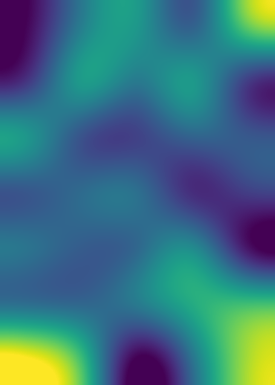
\includegraphics[interpolate=true,width=2.750000in,height=3.850000in]{graph/res/6sensores-img2.png}}%
\end{pgfscope}%
\begin{pgfscope}%
\pgfsetbuttcap%
\pgfsetroundjoin%
\definecolor{currentfill}{rgb}{0.000000,0.000000,0.000000}%
\pgfsetfillcolor{currentfill}%
\pgfsetlinewidth{0.803000pt}%
\definecolor{currentstroke}{rgb}{0.000000,0.000000,0.000000}%
\pgfsetstrokecolor{currentstroke}%
\pgfsetdash{}{0pt}%
\pgfsys@defobject{currentmarker}{\pgfqpoint{0.000000in}{-0.048611in}}{\pgfqpoint{0.000000in}{0.000000in}}{%
\pgfpathmoveto{\pgfqpoint{0.000000in}{0.000000in}}%
\pgfpathlineto{\pgfqpoint{0.000000in}{-0.048611in}}%
\pgfusepath{stroke,fill}%
}%
\begin{pgfscope}%
\pgfsys@transformshift{3.066259in}{0.550000in}%
\pgfsys@useobject{currentmarker}{}%
\end{pgfscope}%
\end{pgfscope}%
\begin{pgfscope}%
\definecolor{textcolor}{rgb}{0.000000,0.000000,0.000000}%
\pgfsetstrokecolor{textcolor}%
\pgfsetfillcolor{textcolor}%
\pgftext[x=3.066259in,y=0.452778in,,top]{\color{textcolor}\rmfamily\fontsize{10.000000}{12.000000}\selectfont -2}%
\end{pgfscope}%
\begin{pgfscope}%
\pgfsetbuttcap%
\pgfsetroundjoin%
\definecolor{currentfill}{rgb}{0.000000,0.000000,0.000000}%
\pgfsetfillcolor{currentfill}%
\pgfsetlinewidth{0.803000pt}%
\definecolor{currentstroke}{rgb}{0.000000,0.000000,0.000000}%
\pgfsetstrokecolor{currentstroke}%
\pgfsetdash{}{0pt}%
\pgfsys@defobject{currentmarker}{\pgfqpoint{0.000000in}{-0.048611in}}{\pgfqpoint{0.000000in}{0.000000in}}{%
\pgfpathmoveto{\pgfqpoint{0.000000in}{0.000000in}}%
\pgfpathlineto{\pgfqpoint{0.000000in}{-0.048611in}}%
\pgfusepath{stroke,fill}%
}%
\begin{pgfscope}%
\pgfsys@transformshift{3.616259in}{0.550000in}%
\pgfsys@useobject{currentmarker}{}%
\end{pgfscope}%
\end{pgfscope}%
\begin{pgfscope}%
\definecolor{textcolor}{rgb}{0.000000,0.000000,0.000000}%
\pgfsetstrokecolor{textcolor}%
\pgfsetfillcolor{textcolor}%
\pgftext[x=3.616259in,y=0.452778in,,top]{\color{textcolor}\rmfamily\fontsize{10.000000}{12.000000}\selectfont -1}%
\end{pgfscope}%
\begin{pgfscope}%
\pgfsetbuttcap%
\pgfsetroundjoin%
\definecolor{currentfill}{rgb}{0.000000,0.000000,0.000000}%
\pgfsetfillcolor{currentfill}%
\pgfsetlinewidth{0.803000pt}%
\definecolor{currentstroke}{rgb}{0.000000,0.000000,0.000000}%
\pgfsetstrokecolor{currentstroke}%
\pgfsetdash{}{0pt}%
\pgfsys@defobject{currentmarker}{\pgfqpoint{0.000000in}{-0.048611in}}{\pgfqpoint{0.000000in}{0.000000in}}{%
\pgfpathmoveto{\pgfqpoint{0.000000in}{0.000000in}}%
\pgfpathlineto{\pgfqpoint{0.000000in}{-0.048611in}}%
\pgfusepath{stroke,fill}%
}%
\begin{pgfscope}%
\pgfsys@transformshift{4.166259in}{0.550000in}%
\pgfsys@useobject{currentmarker}{}%
\end{pgfscope}%
\end{pgfscope}%
\begin{pgfscope}%
\definecolor{textcolor}{rgb}{0.000000,0.000000,0.000000}%
\pgfsetstrokecolor{textcolor}%
\pgfsetfillcolor{textcolor}%
\pgftext[x=4.166259in,y=0.452778in,,top]{\color{textcolor}\rmfamily\fontsize{10.000000}{12.000000}\selectfont 0}%
\end{pgfscope}%
\begin{pgfscope}%
\pgfsetbuttcap%
\pgfsetroundjoin%
\definecolor{currentfill}{rgb}{0.000000,0.000000,0.000000}%
\pgfsetfillcolor{currentfill}%
\pgfsetlinewidth{0.803000pt}%
\definecolor{currentstroke}{rgb}{0.000000,0.000000,0.000000}%
\pgfsetstrokecolor{currentstroke}%
\pgfsetdash{}{0pt}%
\pgfsys@defobject{currentmarker}{\pgfqpoint{0.000000in}{-0.048611in}}{\pgfqpoint{0.000000in}{0.000000in}}{%
\pgfpathmoveto{\pgfqpoint{0.000000in}{0.000000in}}%
\pgfpathlineto{\pgfqpoint{0.000000in}{-0.048611in}}%
\pgfusepath{stroke,fill}%
}%
\begin{pgfscope}%
\pgfsys@transformshift{4.716259in}{0.550000in}%
\pgfsys@useobject{currentmarker}{}%
\end{pgfscope}%
\end{pgfscope}%
\begin{pgfscope}%
\definecolor{textcolor}{rgb}{0.000000,0.000000,0.000000}%
\pgfsetstrokecolor{textcolor}%
\pgfsetfillcolor{textcolor}%
\pgftext[x=4.716259in,y=0.452778in,,top]{\color{textcolor}\rmfamily\fontsize{10.000000}{12.000000}\selectfont 1}%
\end{pgfscope}%
\begin{pgfscope}%
\pgfsetbuttcap%
\pgfsetroundjoin%
\definecolor{currentfill}{rgb}{0.000000,0.000000,0.000000}%
\pgfsetfillcolor{currentfill}%
\pgfsetlinewidth{0.803000pt}%
\definecolor{currentstroke}{rgb}{0.000000,0.000000,0.000000}%
\pgfsetstrokecolor{currentstroke}%
\pgfsetdash{}{0pt}%
\pgfsys@defobject{currentmarker}{\pgfqpoint{0.000000in}{-0.048611in}}{\pgfqpoint{0.000000in}{0.000000in}}{%
\pgfpathmoveto{\pgfqpoint{0.000000in}{0.000000in}}%
\pgfpathlineto{\pgfqpoint{0.000000in}{-0.048611in}}%
\pgfusepath{stroke,fill}%
}%
\begin{pgfscope}%
\pgfsys@transformshift{5.266259in}{0.550000in}%
\pgfsys@useobject{currentmarker}{}%
\end{pgfscope}%
\end{pgfscope}%
\begin{pgfscope}%
\definecolor{textcolor}{rgb}{0.000000,0.000000,0.000000}%
\pgfsetstrokecolor{textcolor}%
\pgfsetfillcolor{textcolor}%
\pgftext[x=5.266259in,y=0.452778in,,top]{\color{textcolor}\rmfamily\fontsize{10.000000}{12.000000}\selectfont 2}%
\end{pgfscope}%
\begin{pgfscope}%
\definecolor{textcolor}{rgb}{0.000000,0.000000,0.000000}%
\pgfsetstrokecolor{textcolor}%
\pgfsetfillcolor{textcolor}%
\pgftext[x=4.166259in,y=0.274567in,,top]{\color{textcolor}\rmfamily\fontsize{10.000000}{12.000000}\selectfont x [m]}%
\end{pgfscope}%
\begin{pgfscope}%
\pgfsetbuttcap%
\pgfsetroundjoin%
\definecolor{currentfill}{rgb}{0.000000,0.000000,0.000000}%
\pgfsetfillcolor{currentfill}%
\pgfsetlinewidth{0.803000pt}%
\definecolor{currentstroke}{rgb}{0.000000,0.000000,0.000000}%
\pgfsetstrokecolor{currentstroke}%
\pgfsetdash{}{0pt}%
\pgfsys@defobject{currentmarker}{\pgfqpoint{-0.048611in}{0.000000in}}{\pgfqpoint{-0.000000in}{0.000000in}}{%
\pgfpathmoveto{\pgfqpoint{-0.000000in}{0.000000in}}%
\pgfpathlineto{\pgfqpoint{-0.048611in}{0.000000in}}%
\pgfusepath{stroke,fill}%
}%
\begin{pgfscope}%
\pgfsys@transformshift{2.791259in}{0.825000in}%
\pgfsys@useobject{currentmarker}{}%
\end{pgfscope}%
\end{pgfscope}%
\begin{pgfscope}%
\definecolor{textcolor}{rgb}{0.000000,0.000000,0.000000}%
\pgfsetstrokecolor{textcolor}%
\pgfsetfillcolor{textcolor}%
\pgftext[x=2.578324in, y=0.777172in, left, base]{\color{textcolor}\rmfamily\fontsize{10.000000}{12.000000}\selectfont -3}%
\end{pgfscope}%
\begin{pgfscope}%
\pgfsetbuttcap%
\pgfsetroundjoin%
\definecolor{currentfill}{rgb}{0.000000,0.000000,0.000000}%
\pgfsetfillcolor{currentfill}%
\pgfsetlinewidth{0.803000pt}%
\definecolor{currentstroke}{rgb}{0.000000,0.000000,0.000000}%
\pgfsetstrokecolor{currentstroke}%
\pgfsetdash{}{0pt}%
\pgfsys@defobject{currentmarker}{\pgfqpoint{-0.048611in}{0.000000in}}{\pgfqpoint{-0.000000in}{0.000000in}}{%
\pgfpathmoveto{\pgfqpoint{-0.000000in}{0.000000in}}%
\pgfpathlineto{\pgfqpoint{-0.048611in}{0.000000in}}%
\pgfusepath{stroke,fill}%
}%
\begin{pgfscope}%
\pgfsys@transformshift{2.791259in}{1.375000in}%
\pgfsys@useobject{currentmarker}{}%
\end{pgfscope}%
\end{pgfscope}%
\begin{pgfscope}%
\definecolor{textcolor}{rgb}{0.000000,0.000000,0.000000}%
\pgfsetstrokecolor{textcolor}%
\pgfsetfillcolor{textcolor}%
\pgftext[x=2.578324in, y=1.327172in, left, base]{\color{textcolor}\rmfamily\fontsize{10.000000}{12.000000}\selectfont -2}%
\end{pgfscope}%
\begin{pgfscope}%
\pgfsetbuttcap%
\pgfsetroundjoin%
\definecolor{currentfill}{rgb}{0.000000,0.000000,0.000000}%
\pgfsetfillcolor{currentfill}%
\pgfsetlinewidth{0.803000pt}%
\definecolor{currentstroke}{rgb}{0.000000,0.000000,0.000000}%
\pgfsetstrokecolor{currentstroke}%
\pgfsetdash{}{0pt}%
\pgfsys@defobject{currentmarker}{\pgfqpoint{-0.048611in}{0.000000in}}{\pgfqpoint{-0.000000in}{0.000000in}}{%
\pgfpathmoveto{\pgfqpoint{-0.000000in}{0.000000in}}%
\pgfpathlineto{\pgfqpoint{-0.048611in}{0.000000in}}%
\pgfusepath{stroke,fill}%
}%
\begin{pgfscope}%
\pgfsys@transformshift{2.791259in}{1.925000in}%
\pgfsys@useobject{currentmarker}{}%
\end{pgfscope}%
\end{pgfscope}%
\begin{pgfscope}%
\definecolor{textcolor}{rgb}{0.000000,0.000000,0.000000}%
\pgfsetstrokecolor{textcolor}%
\pgfsetfillcolor{textcolor}%
\pgftext[x=2.578324in, y=1.877172in, left, base]{\color{textcolor}\rmfamily\fontsize{10.000000}{12.000000}\selectfont -1}%
\end{pgfscope}%
\begin{pgfscope}%
\pgfsetbuttcap%
\pgfsetroundjoin%
\definecolor{currentfill}{rgb}{0.000000,0.000000,0.000000}%
\pgfsetfillcolor{currentfill}%
\pgfsetlinewidth{0.803000pt}%
\definecolor{currentstroke}{rgb}{0.000000,0.000000,0.000000}%
\pgfsetstrokecolor{currentstroke}%
\pgfsetdash{}{0pt}%
\pgfsys@defobject{currentmarker}{\pgfqpoint{-0.048611in}{0.000000in}}{\pgfqpoint{-0.000000in}{0.000000in}}{%
\pgfpathmoveto{\pgfqpoint{-0.000000in}{0.000000in}}%
\pgfpathlineto{\pgfqpoint{-0.048611in}{0.000000in}}%
\pgfusepath{stroke,fill}%
}%
\begin{pgfscope}%
\pgfsys@transformshift{2.791259in}{2.475000in}%
\pgfsys@useobject{currentmarker}{}%
\end{pgfscope}%
\end{pgfscope}%
\begin{pgfscope}%
\definecolor{textcolor}{rgb}{0.000000,0.000000,0.000000}%
\pgfsetstrokecolor{textcolor}%
\pgfsetfillcolor{textcolor}%
\pgftext[x=2.624609in, y=2.427172in, left, base]{\color{textcolor}\rmfamily\fontsize{10.000000}{12.000000}\selectfont 0}%
\end{pgfscope}%
\begin{pgfscope}%
\pgfsetbuttcap%
\pgfsetroundjoin%
\definecolor{currentfill}{rgb}{0.000000,0.000000,0.000000}%
\pgfsetfillcolor{currentfill}%
\pgfsetlinewidth{0.803000pt}%
\definecolor{currentstroke}{rgb}{0.000000,0.000000,0.000000}%
\pgfsetstrokecolor{currentstroke}%
\pgfsetdash{}{0pt}%
\pgfsys@defobject{currentmarker}{\pgfqpoint{-0.048611in}{0.000000in}}{\pgfqpoint{-0.000000in}{0.000000in}}{%
\pgfpathmoveto{\pgfqpoint{-0.000000in}{0.000000in}}%
\pgfpathlineto{\pgfqpoint{-0.048611in}{0.000000in}}%
\pgfusepath{stroke,fill}%
}%
\begin{pgfscope}%
\pgfsys@transformshift{2.791259in}{3.025000in}%
\pgfsys@useobject{currentmarker}{}%
\end{pgfscope}%
\end{pgfscope}%
\begin{pgfscope}%
\definecolor{textcolor}{rgb}{0.000000,0.000000,0.000000}%
\pgfsetstrokecolor{textcolor}%
\pgfsetfillcolor{textcolor}%
\pgftext[x=2.624609in, y=2.977172in, left, base]{\color{textcolor}\rmfamily\fontsize{10.000000}{12.000000}\selectfont 1}%
\end{pgfscope}%
\begin{pgfscope}%
\pgfsetbuttcap%
\pgfsetroundjoin%
\definecolor{currentfill}{rgb}{0.000000,0.000000,0.000000}%
\pgfsetfillcolor{currentfill}%
\pgfsetlinewidth{0.803000pt}%
\definecolor{currentstroke}{rgb}{0.000000,0.000000,0.000000}%
\pgfsetstrokecolor{currentstroke}%
\pgfsetdash{}{0pt}%
\pgfsys@defobject{currentmarker}{\pgfqpoint{-0.048611in}{0.000000in}}{\pgfqpoint{-0.000000in}{0.000000in}}{%
\pgfpathmoveto{\pgfqpoint{-0.000000in}{0.000000in}}%
\pgfpathlineto{\pgfqpoint{-0.048611in}{0.000000in}}%
\pgfusepath{stroke,fill}%
}%
\begin{pgfscope}%
\pgfsys@transformshift{2.791259in}{3.575000in}%
\pgfsys@useobject{currentmarker}{}%
\end{pgfscope}%
\end{pgfscope}%
\begin{pgfscope}%
\definecolor{textcolor}{rgb}{0.000000,0.000000,0.000000}%
\pgfsetstrokecolor{textcolor}%
\pgfsetfillcolor{textcolor}%
\pgftext[x=2.624609in, y=3.527172in, left, base]{\color{textcolor}\rmfamily\fontsize{10.000000}{12.000000}\selectfont 2}%
\end{pgfscope}%
\begin{pgfscope}%
\pgfsetbuttcap%
\pgfsetroundjoin%
\definecolor{currentfill}{rgb}{0.000000,0.000000,0.000000}%
\pgfsetfillcolor{currentfill}%
\pgfsetlinewidth{0.803000pt}%
\definecolor{currentstroke}{rgb}{0.000000,0.000000,0.000000}%
\pgfsetstrokecolor{currentstroke}%
\pgfsetdash{}{0pt}%
\pgfsys@defobject{currentmarker}{\pgfqpoint{-0.048611in}{0.000000in}}{\pgfqpoint{-0.000000in}{0.000000in}}{%
\pgfpathmoveto{\pgfqpoint{-0.000000in}{0.000000in}}%
\pgfpathlineto{\pgfqpoint{-0.048611in}{0.000000in}}%
\pgfusepath{stroke,fill}%
}%
\begin{pgfscope}%
\pgfsys@transformshift{2.791259in}{4.125000in}%
\pgfsys@useobject{currentmarker}{}%
\end{pgfscope}%
\end{pgfscope}%
\begin{pgfscope}%
\definecolor{textcolor}{rgb}{0.000000,0.000000,0.000000}%
\pgfsetstrokecolor{textcolor}%
\pgfsetfillcolor{textcolor}%
\pgftext[x=2.624609in, y=4.077172in, left, base]{\color{textcolor}\rmfamily\fontsize{10.000000}{12.000000}\selectfont 3}%
\end{pgfscope}%
\begin{pgfscope}%
\definecolor{textcolor}{rgb}{0.000000,0.000000,0.000000}%
\pgfsetstrokecolor{textcolor}%
\pgfsetfillcolor{textcolor}%
\pgftext[x=2.522768in,y=2.475000in,,bottom,rotate=90.000000]{\color{textcolor}\rmfamily\fontsize{10.000000}{12.000000}\selectfont y [m]}%
\end{pgfscope}%
\begin{pgfscope}%
\pgfsetrectcap%
\pgfsetmiterjoin%
\pgfsetlinewidth{0.803000pt}%
\definecolor{currentstroke}{rgb}{0.000000,0.000000,0.000000}%
\pgfsetstrokecolor{currentstroke}%
\pgfsetdash{}{0pt}%
\pgfpathmoveto{\pgfqpoint{2.791259in}{0.550000in}}%
\pgfpathlineto{\pgfqpoint{2.791259in}{4.400000in}}%
\pgfusepath{stroke}%
\end{pgfscope}%
\begin{pgfscope}%
\pgfsetrectcap%
\pgfsetmiterjoin%
\pgfsetlinewidth{0.803000pt}%
\definecolor{currentstroke}{rgb}{0.000000,0.000000,0.000000}%
\pgfsetstrokecolor{currentstroke}%
\pgfsetdash{}{0pt}%
\pgfpathmoveto{\pgfqpoint{5.541259in}{0.550000in}}%
\pgfpathlineto{\pgfqpoint{5.541259in}{4.400000in}}%
\pgfusepath{stroke}%
\end{pgfscope}%
\begin{pgfscope}%
\pgfsetrectcap%
\pgfsetmiterjoin%
\pgfsetlinewidth{0.803000pt}%
\definecolor{currentstroke}{rgb}{0.000000,0.000000,0.000000}%
\pgfsetstrokecolor{currentstroke}%
\pgfsetdash{}{0pt}%
\pgfpathmoveto{\pgfqpoint{2.791259in}{0.550000in}}%
\pgfpathlineto{\pgfqpoint{5.541259in}{0.550000in}}%
\pgfusepath{stroke}%
\end{pgfscope}%
\begin{pgfscope}%
\pgfsetrectcap%
\pgfsetmiterjoin%
\pgfsetlinewidth{0.803000pt}%
\definecolor{currentstroke}{rgb}{0.000000,0.000000,0.000000}%
\pgfsetstrokecolor{currentstroke}%
\pgfsetdash{}{0pt}%
\pgfpathmoveto{\pgfqpoint{2.791259in}{4.400000in}}%
\pgfpathlineto{\pgfqpoint{5.541259in}{4.400000in}}%
\pgfusepath{stroke}%
\end{pgfscope}%
\begin{pgfscope}%
\definecolor{textcolor}{rgb}{1.000000,1.000000,1.000000}%
\pgfsetstrokecolor{textcolor}%
\pgfsetfillcolor{textcolor}%
\pgftext[x=2.908118in, y=0.870514in, left, base]{\color{black}\rmfamily\fontsize{10.000000}{12.000000}\selectfont 35.79}%
\end{pgfscope}%
\begin{pgfscope}%
\definecolor{textcolor}{rgb}{1.000000,1.000000,1.000000}%
\pgfsetstrokecolor{textcolor}%
\pgfsetfillcolor{textcolor}%
\pgftext[x=2.888833in, y=0.718545in, left, base]{\color{black}\rmfamily\fontsize{10.000000}{12.000000}\selectfont  (1.82)}%
\end{pgfscope}%
\begin{pgfscope}%
\definecolor{textcolor}{rgb}{1.000000,1.000000,1.000000}%
\pgfsetstrokecolor{textcolor}%
\pgfsetfillcolor{textcolor}%
\pgftext[x=3.458118in, y=0.870514in, left, base]{\color{textcolor}\rmfamily\fontsize{10.000000}{12.000000}\selectfont 26.89}%
\end{pgfscope}%
\begin{pgfscope}%
\definecolor{textcolor}{rgb}{1.000000,1.000000,1.000000}%
\pgfsetstrokecolor{textcolor}%
\pgfsetfillcolor{textcolor}%
\pgftext[x=3.438833in, y=0.718545in, left, base]{\color{textcolor}\rmfamily\fontsize{10.000000}{12.000000}\selectfont  (6.94)}%
\end{pgfscope}%
\begin{pgfscope}%
\definecolor{textcolor}{rgb}{1.000000,1.000000,1.000000}%
\pgfsetstrokecolor{textcolor}%
\pgfsetfillcolor{textcolor}%
\pgftext[x=4.042832in, y=0.870514in, left, base]{\color{textcolor}\rmfamily\fontsize{10.000000}{12.000000}\selectfont 8.67}%
\end{pgfscope}%
\begin{pgfscope}%
\definecolor{textcolor}{rgb}{1.000000,1.000000,1.000000}%
\pgfsetstrokecolor{textcolor}%
\pgfsetfillcolor{textcolor}%
\pgftext[x=3.988833in, y=0.718545in, left, base]{\color{textcolor}\rmfamily\fontsize{10.000000}{12.000000}\selectfont  (4.59)}%
\end{pgfscope}%
\begin{pgfscope}%
\definecolor{textcolor}{rgb}{1.000000,1.000000,1.000000}%
\pgfsetstrokecolor{textcolor}%
\pgfsetfillcolor{textcolor}%
\pgftext[x=4.558118in, y=0.870514in, left, base]{\color{textcolor}\rmfamily\fontsize{10.000000}{12.000000}\selectfont 19.12}%
\end{pgfscope}%
\begin{pgfscope}%
\definecolor{textcolor}{rgb}{1.000000,1.000000,1.000000}%
\pgfsetstrokecolor{textcolor}%
\pgfsetfillcolor{textcolor}%
\pgftext[x=4.538833in, y=0.718545in, left, base]{\color{textcolor}\rmfamily\fontsize{10.000000}{12.000000}\selectfont  (8.27)}%
\end{pgfscope}%
\begin{pgfscope}%
\definecolor{textcolor}{rgb}{1.000000,1.000000,1.000000}%
\pgfsetstrokecolor{textcolor}%
\pgfsetfillcolor{textcolor}%
\pgftext[x=5.108118in, y=0.870514in, left, base]{\color{black}\rmfamily\fontsize{10.000000}{12.000000}\selectfont 32.11}%
\end{pgfscope}%
\begin{pgfscope}%
\definecolor{textcolor}{rgb}{1.000000,1.000000,1.000000}%
\pgfsetstrokecolor{textcolor}%
\pgfsetfillcolor{textcolor}%
\pgftext[x=5.054119in, y=0.718545in, left, base]{\color{black}\rmfamily\fontsize{10.000000}{12.000000}\selectfont  (11.71)}%
\end{pgfscope}%
\begin{pgfscope}%
\definecolor{textcolor}{rgb}{1.000000,1.000000,1.000000}%
\pgfsetstrokecolor{textcolor}%
\pgfsetfillcolor{textcolor}%
\pgftext[x=2.908118in, y=1.420514in, left, base]{\color{textcolor}\rmfamily\fontsize{10.000000}{12.000000}\selectfont 18.22}%
\end{pgfscope}%
\begin{pgfscope}%
\definecolor{textcolor}{rgb}{1.000000,1.000000,1.000000}%
\pgfsetstrokecolor{textcolor}%
\pgfsetfillcolor{textcolor}%
\pgftext[x=2.888833in, y=1.268545in, left, base]{\color{textcolor}\rmfamily\fontsize{10.000000}{12.000000}\selectfont  (2.59)}%
\end{pgfscope}%
\begin{pgfscope}%
\definecolor{textcolor}{rgb}{1.000000,1.000000,1.000000}%
\pgfsetstrokecolor{textcolor}%
\pgfsetfillcolor{textcolor}%
\pgftext[x=3.458118in, y=1.420514in, left, base]{\color{textcolor}\rmfamily\fontsize{10.000000}{12.000000}\selectfont 17.54}%
\end{pgfscope}%
\begin{pgfscope}%
\definecolor{textcolor}{rgb}{1.000000,1.000000,1.000000}%
\pgfsetstrokecolor{textcolor}%
\pgfsetfillcolor{textcolor}%
\pgftext[x=3.473547in, y=1.268545in, left, base]{\color{textcolor}\rmfamily\fontsize{10.000000}{12.000000}\selectfont  (2.9)}%
\end{pgfscope}%
\begin{pgfscope}%
\definecolor{textcolor}{rgb}{1.000000,1.000000,1.000000}%
\pgfsetstrokecolor{textcolor}%
\pgfsetfillcolor{textcolor}%
\pgftext[x=4.042832in, y=1.420514in, left, base]{\color{textcolor}\rmfamily\fontsize{10.000000}{12.000000}\selectfont 19.9}%
\end{pgfscope}%
\begin{pgfscope}%
\definecolor{textcolor}{rgb}{1.000000,1.000000,1.000000}%
\pgfsetstrokecolor{textcolor}%
\pgfsetfillcolor{textcolor}%
\pgftext[x=3.988833in, y=1.268545in, left, base]{\color{textcolor}\rmfamily\fontsize{10.000000}{12.000000}\selectfont  (9.51)}%
\end{pgfscope}%
\begin{pgfscope}%
\definecolor{textcolor}{rgb}{1.000000,1.000000,1.000000}%
\pgfsetstrokecolor{textcolor}%
\pgfsetfillcolor{textcolor}%
\pgftext[x=4.558118in, y=1.420514in, left, base]{\color{textcolor}\rmfamily\fontsize{10.000000}{12.000000}\selectfont 25.32}%
\end{pgfscope}%
\begin{pgfscope}%
\definecolor{textcolor}{rgb}{1.000000,1.000000,1.000000}%
\pgfsetstrokecolor{textcolor}%
\pgfsetfillcolor{textcolor}%
\pgftext[x=4.538833in, y=1.268545in, left, base]{\color{textcolor}\rmfamily\fontsize{10.000000}{12.000000}\selectfont  (9.83)}%
\end{pgfscope}%
\begin{pgfscope}%
\definecolor{textcolor}{rgb}{1.000000,1.000000,1.000000}%
\pgfsetstrokecolor{textcolor}%
\pgfsetfillcolor{textcolor}%
\pgftext[x=5.108118in, y=1.420514in, left, base]{\color{textcolor}\rmfamily\fontsize{10.000000}{12.000000}\selectfont 27.11}%
\end{pgfscope}%
\begin{pgfscope}%
\definecolor{textcolor}{rgb}{1.000000,1.000000,1.000000}%
\pgfsetstrokecolor{textcolor}%
\pgfsetfillcolor{textcolor}%
\pgftext[x=5.088833in, y=1.268545in, left, base]{\color{textcolor}\rmfamily\fontsize{10.000000}{12.000000}\selectfont  (7.62)}%
\end{pgfscope}%
\begin{pgfscope}%
\definecolor{textcolor}{rgb}{1.000000,1.000000,1.000000}%
\pgfsetstrokecolor{textcolor}%
\pgfsetfillcolor{textcolor}%
\pgftext[x=2.908118in, y=1.970514in, left, base]{\color{textcolor}\rmfamily\fontsize{10.000000}{12.000000}\selectfont 19.06}%
\end{pgfscope}%
\begin{pgfscope}%
\definecolor{textcolor}{rgb}{1.000000,1.000000,1.000000}%
\pgfsetstrokecolor{textcolor}%
\pgfsetfillcolor{textcolor}%
\pgftext[x=2.888833in, y=1.818545in, left, base]{\color{textcolor}\rmfamily\fontsize{10.000000}{12.000000}\selectfont  (4.51)}%
\end{pgfscope}%
\begin{pgfscope}%
\definecolor{textcolor}{rgb}{1.000000,1.000000,1.000000}%
\pgfsetstrokecolor{textcolor}%
\pgfsetfillcolor{textcolor}%
\pgftext[x=3.458118in, y=1.970514in, left, base]{\color{textcolor}\rmfamily\fontsize{10.000000}{12.000000}\selectfont 16.58}%
\end{pgfscope}%
\begin{pgfscope}%
\definecolor{textcolor}{rgb}{1.000000,1.000000,1.000000}%
\pgfsetstrokecolor{textcolor}%
\pgfsetfillcolor{textcolor}%
\pgftext[x=3.438833in, y=1.818545in, left, base]{\color{textcolor}\rmfamily\fontsize{10.000000}{12.000000}\selectfont  (3.17)}%
\end{pgfscope}%
\begin{pgfscope}%
\definecolor{textcolor}{rgb}{1.000000,1.000000,1.000000}%
\pgfsetstrokecolor{textcolor}%
\pgfsetfillcolor{textcolor}%
\pgftext[x=4.008118in, y=1.970514in, left, base]{\color{textcolor}\rmfamily\fontsize{10.000000}{12.000000}\selectfont 17.74}%
\end{pgfscope}%
\begin{pgfscope}%
\definecolor{textcolor}{rgb}{1.000000,1.000000,1.000000}%
\pgfsetstrokecolor{textcolor}%
\pgfsetfillcolor{textcolor}%
\pgftext[x=3.988833in, y=1.818545in, left, base]{\color{textcolor}\rmfamily\fontsize{10.000000}{12.000000}\selectfont  (6.96)}%
\end{pgfscope}%
\begin{pgfscope}%
\definecolor{textcolor}{rgb}{1.000000,1.000000,1.000000}%
\pgfsetstrokecolor{textcolor}%
\pgfsetfillcolor{textcolor}%
\pgftext[x=4.592832in, y=1.970514in, left, base]{\color{textcolor}\rmfamily\fontsize{10.000000}{12.000000}\selectfont 21.6}%
\end{pgfscope}%
\begin{pgfscope}%
\definecolor{textcolor}{rgb}{1.000000,1.000000,1.000000}%
\pgfsetstrokecolor{textcolor}%
\pgfsetfillcolor{textcolor}%
\pgftext[x=4.538833in, y=1.818545in, left, base]{\color{textcolor}\rmfamily\fontsize{10.000000}{12.000000}\selectfont  (3.27)}%
\end{pgfscope}%
\begin{pgfscope}%
\definecolor{textcolor}{rgb}{1.000000,1.000000,1.000000}%
\pgfsetstrokecolor{textcolor}%
\pgfsetfillcolor{textcolor}%
\pgftext[x=5.108118in, y=1.970514in, left, base]{\color{textcolor}\rmfamily\fontsize{10.000000}{12.000000}\selectfont 10.25}%
\end{pgfscope}%
\begin{pgfscope}%
\definecolor{textcolor}{rgb}{1.000000,1.000000,1.000000}%
\pgfsetstrokecolor{textcolor}%
\pgfsetfillcolor{textcolor}%
\pgftext[x=5.088833in, y=1.818545in, left, base]{\color{textcolor}\rmfamily\fontsize{10.000000}{12.000000}\selectfont  (1.25)}%
\end{pgfscope}%
\begin{pgfscope}%
\definecolor{textcolor}{rgb}{1.000000,1.000000,1.000000}%
\pgfsetstrokecolor{textcolor}%
\pgfsetfillcolor{textcolor}%
\pgftext[x=2.942832in, y=2.520514in, left, base]{\color{textcolor}\rmfamily\fontsize{10.000000}{12.000000}\selectfont 16.0}%
\end{pgfscope}%
\begin{pgfscope}%
\definecolor{textcolor}{rgb}{1.000000,1.000000,1.000000}%
\pgfsetstrokecolor{textcolor}%
\pgfsetfillcolor{textcolor}%
\pgftext[x=2.888833in, y=2.368545in, left, base]{\color{textcolor}\rmfamily\fontsize{10.000000}{12.000000}\selectfont  (7.24)}%
\end{pgfscope}%
\begin{pgfscope}%
\definecolor{textcolor}{rgb}{1.000000,1.000000,1.000000}%
\pgfsetstrokecolor{textcolor}%
\pgfsetfillcolor{textcolor}%
\pgftext[x=3.458118in, y=2.520514in, left, base]{\color{textcolor}\rmfamily\fontsize{10.000000}{12.000000}\selectfont 18.15}%
\end{pgfscope}%
\begin{pgfscope}%
\definecolor{textcolor}{rgb}{1.000000,1.000000,1.000000}%
\pgfsetstrokecolor{textcolor}%
\pgfsetfillcolor{textcolor}%
\pgftext[x=3.438833in, y=2.368545in, left, base]{\color{textcolor}\rmfamily\fontsize{10.000000}{12.000000}\selectfont  (2.18)}%
\end{pgfscope}%
\begin{pgfscope}%
\definecolor{textcolor}{rgb}{1.000000,1.000000,1.000000}%
\pgfsetstrokecolor{textcolor}%
\pgfsetfillcolor{textcolor}%
\pgftext[x=4.008118in, y=2.520514in, left, base]{\color{textcolor}\rmfamily\fontsize{10.000000}{12.000000}\selectfont 18.62}%
\end{pgfscope}%
\begin{pgfscope}%
\definecolor{textcolor}{rgb}{1.000000,1.000000,1.000000}%
\pgfsetstrokecolor{textcolor}%
\pgfsetfillcolor{textcolor}%
\pgftext[x=3.988833in, y=2.368545in, left, base]{\color{textcolor}\rmfamily\fontsize{10.000000}{12.000000}\selectfont  (5.72)}%
\end{pgfscope}%
\begin{pgfscope}%
\definecolor{textcolor}{rgb}{1.000000,1.000000,1.000000}%
\pgfsetstrokecolor{textcolor}%
\pgfsetfillcolor{textcolor}%
\pgftext[x=4.558118in, y=2.520514in, left, base]{\color{textcolor}\rmfamily\fontsize{10.000000}{12.000000}\selectfont 12.28}%
\end{pgfscope}%
\begin{pgfscope}%
\definecolor{textcolor}{rgb}{1.000000,1.000000,1.000000}%
\pgfsetstrokecolor{textcolor}%
\pgfsetfillcolor{textcolor}%
\pgftext[x=4.538833in, y=2.368545in, left, base]{\color{textcolor}\rmfamily\fontsize{10.000000}{12.000000}\selectfont  (3.57)}%
\end{pgfscope}%
\begin{pgfscope}%
\definecolor{textcolor}{rgb}{1.000000,1.000000,1.000000}%
\pgfsetstrokecolor{textcolor}%
\pgfsetfillcolor{textcolor}%
\pgftext[x=5.108118in, y=2.520514in, left, base]{\color{textcolor}\rmfamily\fontsize{10.000000}{12.000000}\selectfont 13.59}%
\end{pgfscope}%
\begin{pgfscope}%
\definecolor{textcolor}{rgb}{1.000000,1.000000,1.000000}%
\pgfsetstrokecolor{textcolor}%
\pgfsetfillcolor{textcolor}%
\pgftext[x=5.088833in, y=2.368545in, left, base]{\color{textcolor}\rmfamily\fontsize{10.000000}{12.000000}\selectfont  (2.57)}%
\end{pgfscope}%
\begin{pgfscope}%
\definecolor{textcolor}{rgb}{1.000000,1.000000,1.000000}%
\pgfsetstrokecolor{textcolor}%
\pgfsetfillcolor{textcolor}%
\pgftext[x=2.908118in, y=3.070514in, left, base]{\color{textcolor}\rmfamily\fontsize{10.000000}{12.000000}\selectfont 22.85}%
\end{pgfscope}%
\begin{pgfscope}%
\definecolor{textcolor}{rgb}{1.000000,1.000000,1.000000}%
\pgfsetstrokecolor{textcolor}%
\pgfsetfillcolor{textcolor}%
\pgftext[x=2.923547in, y=2.918545in, left, base]{\color{textcolor}\rmfamily\fontsize{10.000000}{12.000000}\selectfont  (5.4)}%
\end{pgfscope}%
\begin{pgfscope}%
\definecolor{textcolor}{rgb}{1.000000,1.000000,1.000000}%
\pgfsetstrokecolor{textcolor}%
\pgfsetfillcolor{textcolor}%
\pgftext[x=3.492832in, y=3.070514in, left, base]{\color{textcolor}\rmfamily\fontsize{10.000000}{12.000000}\selectfont 15.5}%
\end{pgfscope}%
\begin{pgfscope}%
\definecolor{textcolor}{rgb}{1.000000,1.000000,1.000000}%
\pgfsetstrokecolor{textcolor}%
\pgfsetfillcolor{textcolor}%
\pgftext[x=3.438833in, y=2.918545in, left, base]{\color{textcolor}\rmfamily\fontsize{10.000000}{12.000000}\selectfont  (1.12)}%
\end{pgfscope}%
\begin{pgfscope}%
\definecolor{textcolor}{rgb}{1.000000,1.000000,1.000000}%
\pgfsetstrokecolor{textcolor}%
\pgfsetfillcolor{textcolor}%
\pgftext[x=4.008118in, y=3.070514in, left, base]{\color{textcolor}\rmfamily\fontsize{10.000000}{12.000000}\selectfont 14.01}%
\end{pgfscope}%
\begin{pgfscope}%
\definecolor{textcolor}{rgb}{1.000000,1.000000,1.000000}%
\pgfsetstrokecolor{textcolor}%
\pgfsetfillcolor{textcolor}%
\pgftext[x=4.023547in, y=2.918545in, left, base]{\color{textcolor}\rmfamily\fontsize{10.000000}{12.000000}\selectfont  (3.7)}%
\end{pgfscope}%
\begin{pgfscope}%
\definecolor{textcolor}{rgb}{1.000000,1.000000,1.000000}%
\pgfsetstrokecolor{textcolor}%
\pgfsetfillcolor{textcolor}%
\pgftext[x=4.558118in, y=3.070514in, left, base]{\color{textcolor}\rmfamily\fontsize{10.000000}{12.000000}\selectfont 17.11}%
\end{pgfscope}%
\begin{pgfscope}%
\definecolor{textcolor}{rgb}{1.000000,1.000000,1.000000}%
\pgfsetstrokecolor{textcolor}%
\pgfsetfillcolor{textcolor}%
\pgftext[x=4.573547in, y=2.918545in, left, base]{\color{textcolor}\rmfamily\fontsize{10.000000}{12.000000}\selectfont  (6.0)}%
\end{pgfscope}%
\begin{pgfscope}%
\definecolor{textcolor}{rgb}{1.000000,1.000000,1.000000}%
\pgfsetstrokecolor{textcolor}%
\pgfsetfillcolor{textcolor}%
\pgftext[x=5.108118in, y=3.070514in, left, base]{\color{textcolor}\rmfamily\fontsize{10.000000}{12.000000}\selectfont 16.23}%
\end{pgfscope}%
\begin{pgfscope}%
\definecolor{textcolor}{rgb}{1.000000,1.000000,1.000000}%
\pgfsetstrokecolor{textcolor}%
\pgfsetfillcolor{textcolor}%
\pgftext[x=5.088833in, y=2.918545in, left, base]{\color{textcolor}\rmfamily\fontsize{10.000000}{12.000000}\selectfont  (0.02)}%
\end{pgfscope}%
\begin{pgfscope}%
\definecolor{textcolor}{rgb}{1.000000,1.000000,1.000000}%
\pgfsetstrokecolor{textcolor}%
\pgfsetfillcolor{textcolor}%
\pgftext[x=2.908118in, y=3.620514in, left, base]{\color{textcolor}\rmfamily\fontsize{10.000000}{12.000000}\selectfont 13.21}%
\end{pgfscope}%
\begin{pgfscope}%
\definecolor{textcolor}{rgb}{1.000000,1.000000,1.000000}%
\pgfsetstrokecolor{textcolor}%
\pgfsetfillcolor{textcolor}%
\pgftext[x=2.923547in, y=3.468545in, left, base]{\color{textcolor}\rmfamily\fontsize{10.000000}{12.000000}\selectfont  (5.8)}%
\end{pgfscope}%
\begin{pgfscope}%
\definecolor{textcolor}{rgb}{1.000000,1.000000,1.000000}%
\pgfsetstrokecolor{textcolor}%
\pgfsetfillcolor{textcolor}%
\pgftext[x=3.492832in, y=3.620514in, left, base]{\color{textcolor}\rmfamily\fontsize{10.000000}{12.000000}\selectfont 23.4}%
\end{pgfscope}%
\begin{pgfscope}%
\definecolor{textcolor}{rgb}{1.000000,1.000000,1.000000}%
\pgfsetstrokecolor{textcolor}%
\pgfsetfillcolor{textcolor}%
\pgftext[x=3.438833in, y=3.468545in, left, base]{\color{textcolor}\rmfamily\fontsize{10.000000}{12.000000}\selectfont  (2.02)}%
\end{pgfscope}%
\begin{pgfscope}%
\definecolor{textcolor}{rgb}{1.000000,1.000000,1.000000}%
\pgfsetstrokecolor{textcolor}%
\pgfsetfillcolor{textcolor}%
\pgftext[x=4.008118in, y=3.620514in, left, base]{\color{textcolor}\rmfamily\fontsize{10.000000}{12.000000}\selectfont 19.58}%
\end{pgfscope}%
\begin{pgfscope}%
\definecolor{textcolor}{rgb}{1.000000,1.000000,1.000000}%
\pgfsetstrokecolor{textcolor}%
\pgfsetfillcolor{textcolor}%
\pgftext[x=3.988833in, y=3.468545in, left, base]{\color{textcolor}\rmfamily\fontsize{10.000000}{12.000000}\selectfont  (6.48)}%
\end{pgfscope}%
\begin{pgfscope}%
\definecolor{textcolor}{rgb}{1.000000,1.000000,1.000000}%
\pgfsetstrokecolor{textcolor}%
\pgfsetfillcolor{textcolor}%
\pgftext[x=4.558118in, y=3.620514in, left, base]{\color{textcolor}\rmfamily\fontsize{10.000000}{12.000000}\selectfont 23.25}%
\end{pgfscope}%
\begin{pgfscope}%
\definecolor{textcolor}{rgb}{1.000000,1.000000,1.000000}%
\pgfsetstrokecolor{textcolor}%
\pgfsetfillcolor{textcolor}%
\pgftext[x=4.538833in, y=3.468545in, left, base]{\color{textcolor}\rmfamily\fontsize{10.000000}{12.000000}\selectfont  (2.06)}%
\end{pgfscope}%
\begin{pgfscope}%
\definecolor{textcolor}{rgb}{1.000000,1.000000,1.000000}%
\pgfsetstrokecolor{textcolor}%
\pgfsetfillcolor{textcolor}%
\pgftext[x=5.108118in, y=3.620514in, left, base]{\color{textcolor}\rmfamily\fontsize{10.000000}{12.000000}\selectfont 13.43}%
\end{pgfscope}%
\begin{pgfscope}%
\definecolor{textcolor}{rgb}{1.000000,1.000000,1.000000}%
\pgfsetstrokecolor{textcolor}%
\pgfsetfillcolor{textcolor}%
\pgftext[x=5.088833in, y=3.468545in, left, base]{\color{textcolor}\rmfamily\fontsize{10.000000}{12.000000}\selectfont  (3.99)}%
\end{pgfscope}%
\begin{pgfscope}%
\definecolor{textcolor}{rgb}{1.000000,1.000000,1.000000}%
\pgfsetstrokecolor{textcolor}%
\pgfsetfillcolor{textcolor}%
\pgftext[x=2.977546in, y=4.170514in, left, base]{\color{textcolor}\rmfamily\fontsize{10.000000}{12.000000}\selectfont 9.1}%
\end{pgfscope}%
\begin{pgfscope}%
\definecolor{textcolor}{rgb}{1.000000,1.000000,1.000000}%
\pgfsetstrokecolor{textcolor}%
\pgfsetfillcolor{textcolor}%
\pgftext[x=2.888833in, y=4.018545in, left, base]{\color{textcolor}\rmfamily\fontsize{10.000000}{12.000000}\selectfont  (3.65)}%
\end{pgfscope}%
\begin{pgfscope}%
\definecolor{textcolor}{rgb}{1.000000,1.000000,1.000000}%
\pgfsetstrokecolor{textcolor}%
\pgfsetfillcolor{textcolor}%
\pgftext[x=3.458118in, y=4.170514in, left, base]{\color{textcolor}\rmfamily\fontsize{10.000000}{12.000000}\selectfont 20.42}%
\end{pgfscope}%
\begin{pgfscope}%
\definecolor{textcolor}{rgb}{1.000000,1.000000,1.000000}%
\pgfsetstrokecolor{textcolor}%
\pgfsetfillcolor{textcolor}%
\pgftext[x=3.438833in, y=4.018545in, left, base]{\color{textcolor}\rmfamily\fontsize{10.000000}{12.000000}\selectfont  (4.14)}%
\end{pgfscope}%
\begin{pgfscope}%
\definecolor{textcolor}{rgb}{1.000000,1.000000,1.000000}%
\pgfsetstrokecolor{textcolor}%
\pgfsetfillcolor{textcolor}%
\pgftext[x=4.008118in, y=4.170514in, left, base]{\color{textcolor}\rmfamily\fontsize{10.000000}{12.000000}\selectfont 22.95}%
\end{pgfscope}%
\begin{pgfscope}%
\definecolor{textcolor}{rgb}{1.000000,1.000000,1.000000}%
\pgfsetstrokecolor{textcolor}%
\pgfsetfillcolor{textcolor}%
\pgftext[x=4.023547in, y=4.018545in, left, base]{\color{textcolor}\rmfamily\fontsize{10.000000}{12.000000}\selectfont  (2.1)}%
\end{pgfscope}%
\begin{pgfscope}%
\definecolor{textcolor}{rgb}{1.000000,1.000000,1.000000}%
\pgfsetstrokecolor{textcolor}%
\pgfsetfillcolor{textcolor}%
\pgftext[x=4.558118in, y=4.170514in, left, base]{\color{textcolor}\rmfamily\fontsize{10.000000}{12.000000}\selectfont 17.28}%
\end{pgfscope}%
\begin{pgfscope}%
\definecolor{textcolor}{rgb}{1.000000,1.000000,1.000000}%
\pgfsetstrokecolor{textcolor}%
\pgfsetfillcolor{textcolor}%
\pgftext[x=4.538833in, y=4.018545in, left, base]{\color{textcolor}\rmfamily\fontsize{10.000000}{12.000000}\selectfont  (5.93)}%
\end{pgfscope}%
\begin{pgfscope}%
\definecolor{textcolor}{rgb}{1.000000,1.000000,1.000000}%
\pgfsetstrokecolor{textcolor}%
\pgfsetfillcolor{textcolor}%
\pgftext[x=5.142832in, y=4.170514in, left, base]{\color{textcolor}\rmfamily\fontsize{10.000000}{12.000000}\selectfont 28.8}%
\end{pgfscope}%
\begin{pgfscope}%
\definecolor{textcolor}{rgb}{1.000000,1.000000,1.000000}%
\pgfsetstrokecolor{textcolor}%
\pgfsetfillcolor{textcolor}%
\pgftext[x=5.088833in, y=4.018545in, left, base]{\color{textcolor}\rmfamily\fontsize{10.000000}{12.000000}\selectfont  (12.3)}%
\end{pgfscope}%
\begin{pgfscope}%
\definecolor{textcolor}{rgb}{0.000000,0.000000,0.000000}%
\pgfsetstrokecolor{textcolor}%
\pgfsetfillcolor{textcolor}%
\pgftext[x=4.166259in,y=4.483333in,,base]{\color{textcolor}\rmfamily\fontsize{12.000000}{14.400000}\selectfont Posición}%
\end{pgfscope}%
\begin{pgfscope}%
\pgfpathrectangle{\pgfqpoint{5.730944in}{0.742500in}}{\pgfqpoint{0.173250in}{3.465000in}}%
\pgfusepath{clip}%
\pgfsetbuttcap%
\pgfsetmiterjoin%
\definecolor{currentfill}{rgb}{1.000000,1.000000,1.000000}%
\pgfsetfillcolor{currentfill}%
\pgfsetlinewidth{0.010037pt}%
\definecolor{currentstroke}{rgb}{1.000000,1.000000,1.000000}%
\pgfsetstrokecolor{currentstroke}%
\pgfsetdash{}{0pt}%
\pgfpathmoveto{\pgfqpoint{5.730944in}{0.742500in}}%
\pgfpathlineto{\pgfqpoint{5.730944in}{0.756035in}}%
\pgfpathlineto{\pgfqpoint{5.730944in}{4.193965in}}%
\pgfpathlineto{\pgfqpoint{5.730944in}{4.207500in}}%
\pgfpathlineto{\pgfqpoint{5.904194in}{4.207500in}}%
\pgfpathlineto{\pgfqpoint{5.904194in}{4.193965in}}%
\pgfpathlineto{\pgfqpoint{5.904194in}{0.756035in}}%
\pgfpathlineto{\pgfqpoint{5.904194in}{0.742500in}}%
\pgfpathclose%
\pgfusepath{stroke,fill}%
\end{pgfscope}%
\begin{pgfscope}%
\pgfsys@transformshift{5.730000in}{0.740000in}%
\pgftext[left,bottom]{
\includegraphics[interpolate=true,width=0.170000in,height=3.470000in]{graph/res/6sensores-img3.png}}%
\end{pgfscope}%
\begin{pgfscope}%
\pgfsetbuttcap%
\pgfsetroundjoin%
\definecolor{currentfill}{rgb}{0.000000,0.000000,0.000000}%
\pgfsetfillcolor{currentfill}%
\pgfsetlinewidth{0.803000pt}%
\definecolor{currentstroke}{rgb}{0.000000,0.000000,0.000000}%
\pgfsetstrokecolor{currentstroke}%
\pgfsetdash{}{0pt}%
\pgfsys@defobject{currentmarker}{\pgfqpoint{0.000000in}{0.000000in}}{\pgfqpoint{0.048611in}{0.000000in}}{%
\pgfpathmoveto{\pgfqpoint{0.000000in}{0.000000in}}%
\pgfpathlineto{\pgfqpoint{0.048611in}{0.000000in}}%
\pgfusepath{stroke,fill}%
}%
\begin{pgfscope}%
\pgfsys@transformshift{5.904194in}{0.912367in}%
\pgfsys@useobject{currentmarker}{}%
\end{pgfscope}%
\end{pgfscope}%
\begin{pgfscope}%
\definecolor{textcolor}{rgb}{0.000000,0.000000,0.000000}%
\pgfsetstrokecolor{textcolor}%
\pgfsetfillcolor{textcolor}%
\pgftext[x=6.001416in, y=0.864540in, left, base]{\color{textcolor}\rmfamily\fontsize{10.000000}{12.000000}\selectfont \(\displaystyle {10}\)}%
\end{pgfscope}%
\begin{pgfscope}%
\pgfsetbuttcap%
\pgfsetroundjoin%
\definecolor{currentfill}{rgb}{0.000000,0.000000,0.000000}%
\pgfsetfillcolor{currentfill}%
\pgfsetlinewidth{0.803000pt}%
\definecolor{currentstroke}{rgb}{0.000000,0.000000,0.000000}%
\pgfsetstrokecolor{currentstroke}%
\pgfsetdash{}{0pt}%
\pgfsys@defobject{currentmarker}{\pgfqpoint{0.000000in}{0.000000in}}{\pgfqpoint{0.048611in}{0.000000in}}{%
\pgfpathmoveto{\pgfqpoint{0.000000in}{0.000000in}}%
\pgfpathlineto{\pgfqpoint{0.048611in}{0.000000in}}%
\pgfusepath{stroke,fill}%
}%
\begin{pgfscope}%
\pgfsys@transformshift{5.904194in}{1.551170in}%
\pgfsys@useobject{currentmarker}{}%
\end{pgfscope}%
\end{pgfscope}%
\begin{pgfscope}%
\definecolor{textcolor}{rgb}{0.000000,0.000000,0.000000}%
\pgfsetstrokecolor{textcolor}%
\pgfsetfillcolor{textcolor}%
\pgftext[x=6.001416in, y=1.503342in, left, base]{\color{textcolor}\rmfamily\fontsize{10.000000}{12.000000}\selectfont \(\displaystyle {15}\)}%
\end{pgfscope}%
\begin{pgfscope}%
\pgfsetbuttcap%
\pgfsetroundjoin%
\definecolor{currentfill}{rgb}{0.000000,0.000000,0.000000}%
\pgfsetfillcolor{currentfill}%
\pgfsetlinewidth{0.803000pt}%
\definecolor{currentstroke}{rgb}{0.000000,0.000000,0.000000}%
\pgfsetstrokecolor{currentstroke}%
\pgfsetdash{}{0pt}%
\pgfsys@defobject{currentmarker}{\pgfqpoint{0.000000in}{0.000000in}}{\pgfqpoint{0.048611in}{0.000000in}}{%
\pgfpathmoveto{\pgfqpoint{0.000000in}{0.000000in}}%
\pgfpathlineto{\pgfqpoint{0.048611in}{0.000000in}}%
\pgfusepath{stroke,fill}%
}%
\begin{pgfscope}%
\pgfsys@transformshift{5.904194in}{2.189973in}%
\pgfsys@useobject{currentmarker}{}%
\end{pgfscope}%
\end{pgfscope}%
\begin{pgfscope}%
\definecolor{textcolor}{rgb}{0.000000,0.000000,0.000000}%
\pgfsetstrokecolor{textcolor}%
\pgfsetfillcolor{textcolor}%
\pgftext[x=6.001416in, y=2.142145in, left, base]{\color{textcolor}\rmfamily\fontsize{10.000000}{12.000000}\selectfont \(\displaystyle {20}\)}%
\end{pgfscope}%
\begin{pgfscope}%
\pgfsetbuttcap%
\pgfsetroundjoin%
\definecolor{currentfill}{rgb}{0.000000,0.000000,0.000000}%
\pgfsetfillcolor{currentfill}%
\pgfsetlinewidth{0.803000pt}%
\definecolor{currentstroke}{rgb}{0.000000,0.000000,0.000000}%
\pgfsetstrokecolor{currentstroke}%
\pgfsetdash{}{0pt}%
\pgfsys@defobject{currentmarker}{\pgfqpoint{0.000000in}{0.000000in}}{\pgfqpoint{0.048611in}{0.000000in}}{%
\pgfpathmoveto{\pgfqpoint{0.000000in}{0.000000in}}%
\pgfpathlineto{\pgfqpoint{0.048611in}{0.000000in}}%
\pgfusepath{stroke,fill}%
}%
\begin{pgfscope}%
\pgfsys@transformshift{5.904194in}{2.828775in}%
\pgfsys@useobject{currentmarker}{}%
\end{pgfscope}%
\end{pgfscope}%
\begin{pgfscope}%
\definecolor{textcolor}{rgb}{0.000000,0.000000,0.000000}%
\pgfsetstrokecolor{textcolor}%
\pgfsetfillcolor{textcolor}%
\pgftext[x=6.001416in, y=2.780948in, left, base]{\color{textcolor}\rmfamily\fontsize{10.000000}{12.000000}\selectfont \(\displaystyle {25}\)}%
\end{pgfscope}%
\begin{pgfscope}%
\pgfsetbuttcap%
\pgfsetroundjoin%
\definecolor{currentfill}{rgb}{0.000000,0.000000,0.000000}%
\pgfsetfillcolor{currentfill}%
\pgfsetlinewidth{0.803000pt}%
\definecolor{currentstroke}{rgb}{0.000000,0.000000,0.000000}%
\pgfsetstrokecolor{currentstroke}%
\pgfsetdash{}{0pt}%
\pgfsys@defobject{currentmarker}{\pgfqpoint{0.000000in}{0.000000in}}{\pgfqpoint{0.048611in}{0.000000in}}{%
\pgfpathmoveto{\pgfqpoint{0.000000in}{0.000000in}}%
\pgfpathlineto{\pgfqpoint{0.048611in}{0.000000in}}%
\pgfusepath{stroke,fill}%
}%
\begin{pgfscope}%
\pgfsys@transformshift{5.904194in}{3.467578in}%
\pgfsys@useobject{currentmarker}{}%
\end{pgfscope}%
\end{pgfscope}%
\begin{pgfscope}%
\definecolor{textcolor}{rgb}{0.000000,0.000000,0.000000}%
\pgfsetstrokecolor{textcolor}%
\pgfsetfillcolor{textcolor}%
\pgftext[x=6.001416in, y=3.419750in, left, base]{\color{textcolor}\rmfamily\fontsize{10.000000}{12.000000}\selectfont \(\displaystyle {30}\)}%
\end{pgfscope}%
\begin{pgfscope}%
\pgfsetbuttcap%
\pgfsetroundjoin%
\definecolor{currentfill}{rgb}{0.000000,0.000000,0.000000}%
\pgfsetfillcolor{currentfill}%
\pgfsetlinewidth{0.803000pt}%
\definecolor{currentstroke}{rgb}{0.000000,0.000000,0.000000}%
\pgfsetstrokecolor{currentstroke}%
\pgfsetdash{}{0pt}%
\pgfsys@defobject{currentmarker}{\pgfqpoint{0.000000in}{0.000000in}}{\pgfqpoint{0.048611in}{0.000000in}}{%
\pgfpathmoveto{\pgfqpoint{0.000000in}{0.000000in}}%
\pgfpathlineto{\pgfqpoint{0.048611in}{0.000000in}}%
\pgfusepath{stroke,fill}%
}%
\begin{pgfscope}%
\pgfsys@transformshift{5.904194in}{4.106381in}%
\pgfsys@useobject{currentmarker}{}%
\end{pgfscope}%
\end{pgfscope}%
\begin{pgfscope}%
\definecolor{textcolor}{rgb}{0.000000,0.000000,0.000000}%
\pgfsetstrokecolor{textcolor}%
\pgfsetfillcolor{textcolor}%
\pgftext[x=6.001416in, y=4.058553in, left, base]{\color{textcolor}\rmfamily\fontsize{10.000000}{12.000000}\selectfont \(\displaystyle {35}\)}%
\end{pgfscope}%
\begin{pgfscope}%
\definecolor{textcolor}{rgb}{0.000000,0.000000,0.000000}%
\pgfsetstrokecolor{textcolor}%
\pgfsetfillcolor{textcolor}%
\pgftext[x=6.348639in,y=2.475000in,,top,rotate=270.000000]{\color{textcolor}\rmfamily\fontsize{10.000000}{12.000000}\selectfont Diferencia de posición [cm]}%
\end{pgfscope}%
\begin{pgfscope}%
\pgfsetbuttcap%
\pgfsetmiterjoin%
\pgfsetlinewidth{0.803000pt}%
\definecolor{currentstroke}{rgb}{0.000000,0.000000,0.000000}%
\pgfsetstrokecolor{currentstroke}%
\pgfsetdash{}{0pt}%
\pgfpathmoveto{\pgfqpoint{5.730944in}{0.742500in}}%
\pgfpathlineto{\pgfqpoint{5.730944in}{0.756035in}}%
\pgfpathlineto{\pgfqpoint{5.730944in}{4.193965in}}%
\pgfpathlineto{\pgfqpoint{5.730944in}{4.207500in}}%
\pgfpathlineto{\pgfqpoint{5.904194in}{4.207500in}}%
\pgfpathlineto{\pgfqpoint{5.904194in}{4.193965in}}%
\pgfpathlineto{\pgfqpoint{5.904194in}{0.756035in}}%
\pgfpathlineto{\pgfqpoint{5.904194in}{0.742500in}}%
\pgfpathclose%
\pgfusepath{stroke}%
\end{pgfscope}%
\begin{pgfscope}%
\pgfpathrectangle{\pgfqpoint{0.305944in}{1.453636in}}{\pgfqpoint{0.113811in}{2.390035in}}%
\pgfusepath{clip}%
\pgfsetbuttcap%
\pgfsetmiterjoin%
\definecolor{currentfill}{rgb}{1.000000,1.000000,1.000000}%
\pgfsetfillcolor{currentfill}%
\pgfsetlinewidth{0.010037pt}%
\definecolor{currentstroke}{rgb}{1.000000,1.000000,1.000000}%
\pgfsetstrokecolor{currentstroke}%
\pgfsetdash{}{0pt}%
\pgfpathmoveto{\pgfqpoint{0.305944in}{1.453636in}}%
\pgfpathlineto{\pgfqpoint{0.305944in}{1.462972in}}%
\pgfpathlineto{\pgfqpoint{0.305944in}{3.834335in}}%
\pgfpathlineto{\pgfqpoint{0.305944in}{3.843671in}}%
\pgfpathlineto{\pgfqpoint{0.419755in}{3.843671in}}%
\pgfpathlineto{\pgfqpoint{0.419755in}{3.834335in}}%
\pgfpathlineto{\pgfqpoint{0.419755in}{1.462972in}}%
\pgfpathlineto{\pgfqpoint{0.419755in}{1.453636in}}%
\pgfpathclose%
\pgfusepath{stroke,fill}%
\end{pgfscope}%
\begin{pgfscope}%
\pgfsys@transformshift{0.310000in}{1.450000in}%
\pgftext[left,bottom]{
\includegraphics[interpolate=true,width=0.110000in,height=2.390000in]{graph/res/6sensores-img4.png}}%
\end{pgfscope}%
\begin{pgfscope}%
\pgfsetbuttcap%
\pgfsetroundjoin%
\definecolor{currentfill}{rgb}{0.000000,0.000000,0.000000}%
\pgfsetfillcolor{currentfill}%
\pgfsetlinewidth{0.803000pt}%
\definecolor{currentstroke}{rgb}{0.000000,0.000000,0.000000}%
\pgfsetstrokecolor{currentstroke}%
\pgfsetdash{}{0pt}%
\pgfsys@defobject{currentmarker}{\pgfqpoint{0.000000in}{0.000000in}}{\pgfqpoint{0.048611in}{0.000000in}}{%
\pgfpathmoveto{\pgfqpoint{0.000000in}{0.000000in}}%
\pgfpathlineto{\pgfqpoint{0.048611in}{0.000000in}}%
\pgfusepath{stroke,fill}%
}%
\begin{pgfscope}%
\pgfsys@transformshift{0.419755in}{1.638454in}%
\pgfsys@useobject{currentmarker}{}%
\end{pgfscope}%
\end{pgfscope}%
\begin{pgfscope}%
\definecolor{textcolor}{rgb}{0.000000,0.000000,0.000000}%
\pgfsetstrokecolor{textcolor}%
\pgfsetfillcolor{textcolor}%
\pgftext[x=0.516977in, y=1.590626in, left, base]{\color{textcolor}\rmfamily\fontsize{10.000000}{12.000000}\selectfont \(\displaystyle {−30}\)}%
\end{pgfscope}%
\begin{pgfscope}%
\pgfsetbuttcap%
\pgfsetroundjoin%
\definecolor{currentfill}{rgb}{0.000000,0.000000,0.000000}%
\pgfsetfillcolor{currentfill}%
\pgfsetlinewidth{0.803000pt}%
\definecolor{currentstroke}{rgb}{0.000000,0.000000,0.000000}%
\pgfsetstrokecolor{currentstroke}%
\pgfsetdash{}{0pt}%
\pgfsys@defobject{currentmarker}{\pgfqpoint{0.000000in}{0.000000in}}{\pgfqpoint{0.048611in}{0.000000in}}{%
\pgfpathmoveto{\pgfqpoint{0.000000in}{0.000000in}}%
\pgfpathlineto{\pgfqpoint{0.048611in}{0.000000in}}%
\pgfusepath{stroke,fill}%
}%
\begin{pgfscope}%
\pgfsys@transformshift{0.419755in}{2.103486in}%
\pgfsys@useobject{currentmarker}{}%
\end{pgfscope}%
\end{pgfscope}%
\begin{pgfscope}%
\definecolor{textcolor}{rgb}{0.000000,0.000000,0.000000}%
\pgfsetstrokecolor{textcolor}%
\pgfsetfillcolor{textcolor}%
\pgftext[x=0.516977in, y=2.055658in, left, base]{\color{textcolor}\rmfamily\fontsize{10.000000}{12.000000}\selectfont \(\displaystyle {−20}\)}%
\end{pgfscope}%
\begin{pgfscope}%
\pgfsetbuttcap%
\pgfsetroundjoin%
\definecolor{currentfill}{rgb}{0.000000,0.000000,0.000000}%
\pgfsetfillcolor{currentfill}%
\pgfsetlinewidth{0.803000pt}%
\definecolor{currentstroke}{rgb}{0.000000,0.000000,0.000000}%
\pgfsetstrokecolor{currentstroke}%
\pgfsetdash{}{0pt}%
\pgfsys@defobject{currentmarker}{\pgfqpoint{0.000000in}{0.000000in}}{\pgfqpoint{0.048611in}{0.000000in}}{%
\pgfpathmoveto{\pgfqpoint{0.000000in}{0.000000in}}%
\pgfpathlineto{\pgfqpoint{0.048611in}{0.000000in}}%
\pgfusepath{stroke,fill}%
}%
\begin{pgfscope}%
\pgfsys@transformshift{0.419755in}{2.568517in}%
\pgfsys@useobject{currentmarker}{}%
\end{pgfscope}%
\end{pgfscope}%
\begin{pgfscope}%
\definecolor{textcolor}{rgb}{0.000000,0.000000,0.000000}%
\pgfsetstrokecolor{textcolor}%
\pgfsetfillcolor{textcolor}%
\pgftext[x=0.516977in, y=2.520689in, left, base]{\color{textcolor}\rmfamily\fontsize{10.000000}{12.000000}\selectfont \(\displaystyle {−10}\)}%
\end{pgfscope}%
\begin{pgfscope}%
\pgfsetbuttcap%
\pgfsetroundjoin%
\definecolor{currentfill}{rgb}{0.000000,0.000000,0.000000}%
\pgfsetfillcolor{currentfill}%
\pgfsetlinewidth{0.803000pt}%
\definecolor{currentstroke}{rgb}{0.000000,0.000000,0.000000}%
\pgfsetstrokecolor{currentstroke}%
\pgfsetdash{}{0pt}%
\pgfsys@defobject{currentmarker}{\pgfqpoint{0.000000in}{0.000000in}}{\pgfqpoint{0.048611in}{0.000000in}}{%
\pgfpathmoveto{\pgfqpoint{0.000000in}{0.000000in}}%
\pgfpathlineto{\pgfqpoint{0.048611in}{0.000000in}}%
\pgfusepath{stroke,fill}%
}%
\begin{pgfscope}%
\pgfsys@transformshift{0.419755in}{3.033549in}%
\pgfsys@useobject{currentmarker}{}%
\end{pgfscope}%
\end{pgfscope}%
\begin{pgfscope}%
\definecolor{textcolor}{rgb}{0.000000,0.000000,0.000000}%
\pgfsetstrokecolor{textcolor}%
\pgfsetfillcolor{textcolor}%
\pgftext[x=0.516977in, y=2.985721in, left, base]{\color{textcolor}\rmfamily\fontsize{10.000000}{12.000000}\selectfont \(\displaystyle {0}\)}%
\end{pgfscope}%
\begin{pgfscope}%
\pgfsetbuttcap%
\pgfsetroundjoin%
\definecolor{currentfill}{rgb}{0.000000,0.000000,0.000000}%
\pgfsetfillcolor{currentfill}%
\pgfsetlinewidth{0.803000pt}%
\definecolor{currentstroke}{rgb}{0.000000,0.000000,0.000000}%
\pgfsetstrokecolor{currentstroke}%
\pgfsetdash{}{0pt}%
\pgfsys@defobject{currentmarker}{\pgfqpoint{0.000000in}{0.000000in}}{\pgfqpoint{0.048611in}{0.000000in}}{%
\pgfpathmoveto{\pgfqpoint{0.000000in}{0.000000in}}%
\pgfpathlineto{\pgfqpoint{0.048611in}{0.000000in}}%
\pgfusepath{stroke,fill}%
}%
\begin{pgfscope}%
\pgfsys@transformshift{0.419755in}{3.498580in}%
\pgfsys@useobject{currentmarker}{}%
\end{pgfscope}%
\end{pgfscope}%
\begin{pgfscope}%
\definecolor{textcolor}{rgb}{0.000000,0.000000,0.000000}%
\pgfsetstrokecolor{textcolor}%
\pgfsetfillcolor{textcolor}%
\pgftext[x=0.516977in, y=3.450752in, left, base]{\color{textcolor}\rmfamily\fontsize{10.000000}{12.000000}\selectfont \(\displaystyle {10}\)}%
\end{pgfscope}%
\begin{pgfscope}%
\definecolor{textcolor}{rgb}{0.000000,0.000000,0.000000}%
\pgfsetstrokecolor{textcolor}%
\pgfsetfillcolor{textcolor}%
\pgftext[x=0.069447in,y=2.648654in,,top,rotate=90.000000]{\color{textcolor}\rmfamily\fontsize{10.000000}{12.000000}\selectfont Diferencia en la medida de cada eje [cm]}%
\end{pgfscope}%
\begin{pgfscope}%
\pgfsetbuttcap%
\pgfsetmiterjoin%
\pgfsetlinewidth{0.803000pt}%
\definecolor{currentstroke}{rgb}{0.000000,0.000000,0.000000}%
\pgfsetstrokecolor{currentstroke}%
\pgfsetdash{}{0pt}%
\pgfpathmoveto{\pgfqpoint{0.305944in}{1.453636in}}%
\pgfpathlineto{\pgfqpoint{0.305944in}{1.462972in}}%
\pgfpathlineto{\pgfqpoint{0.305944in}{3.834335in}}%
\pgfpathlineto{\pgfqpoint{0.305944in}{3.843671in}}%
\pgfpathlineto{\pgfqpoint{0.419755in}{3.843671in}}%
\pgfpathlineto{\pgfqpoint{0.419755in}{3.834335in}}%
\pgfpathlineto{\pgfqpoint{0.419755in}{1.462972in}}%
\pgfpathlineto{\pgfqpoint{0.419755in}{1.453636in}}%
\pgfpathclose%
\pgfusepath{stroke}%
\end{pgfscope}%
\end{pgfpicture}%
\makeatother%
\endgroup%

    \caption{Resultados de las medidas del laboratorio con 6 balizas. Entre paréntesis se indica la desviación estándar de los errores obtenidos en cada punto.}
    \label{fig:res_lab}
\end{figure}


\begin{table}[H]
    \centering
    \hspace*{-0.5cm}
    \begin{tabular}{c|c|c|c|c|c|}
    \cline{2-6}
                                     & \begin{tabular}[c]{@{}c@{}}Error en \\ eje $x$ (cm) \end{tabular} & \begin{tabular}[c]{@{}c@{}} Error en \\ eje $y$ (cm) \end{tabular} & \begin{tabular}[c]{@{}c@{}} Error en eje $x$ \\ (absoluto) (cm) \end{tabular} & \begin{tabular}[c]{@{}c@{}} Error en eje $y$ \\ (absoluto) (cm) \end{tabular} & \begin{tabular}[c]{@{}c@{}} Error en \\ posición(cm) \end{tabular}\\ \hline
    \multicolumn{1}{|c|}{Media}      & -3.7  & 0.7  &  9.6 &  7.7  &  19.2   \\ \hline
    \multicolumn{1}{|c|}{Mediana}    & -2.2  & 2.08  &  8.8 &  6.0  &  18.2   \\ \hline
    \multicolumn{1}{|c|}{Desv. estándar} & 11.0  &  10.3  & 6.5 & 6.8 &  6.1    \\ \hline
    \multicolumn{1}{|c|}{Máximo}     & 15.9  & 17.4  & 24.9 & 33.9 & 35.8   \\ \hline
    \multicolumn{1}{|c|}{Mínimo}     & -24.9 & -33.9 & 0.1 & 0.1 &  8.6    \\ \hline
    \end{tabular}
    \caption{Resumen de los errores en el laboratorio con 6 balizas.}
\end{table}

Los resultados de la toma de medidas con 6 balizas no suponen un cambio especialmente significativo en cuanto a los valores medios de las discrepancias en el posicionamiento, algo esperable teniendo en cuenta que el kit sigue utilizando solo 4 de las balizas en todo momento y las distancias entre sensores no llegan en ningún punto a ser excesivamente altas.

Sí que se puede observar no obstante una mejora en la desviación de las medidas, haciéndolas más estables.
Esto se debe principalmente a la menor distancia entre las balizas y el objetivo en todos los puntos, fruto de una distribución más uniforme de dichas balizas.
% Esto se debe a dos factores: el primero es una distancia, en general, menor entre el objetivo y las balizas que lo posicionan; y por otro lado la distribución más uniforme de dichas balizas, lo que hace que los ángulos definidos entre ellas y el objetivo no sean especialmente agudos, lo que resulta en un pobre rendimiento al realizar los cálculos por triliteración \cite{Simedroni}.

\begin{figure}[H]
  \centering
    \begin{subfigure}[b]{.3\textwidth}
      \centering
      \hspace*{-0.8cm}
      \begin{tikzpicture}
    \begin{axis}[
        ylabel = {Error[cm]},
        x = 0.35\textwidth,
        boxplot/draw direction=y,
        ymajorgrids,
        xtick={1,2},
        xticklabels={4 bal., 6 bal.},
        ]
        \addplot+ [boxplot] table[y index=0] {data/4sens_lab.txt};
        \addplot+ [boxplot] table[y index=0] {data/6sens_lab.txt};
        % \addplot+ [boxplot] table[y index=0] {data/4sens_lab_full.txt};
        % \addplot+ [boxplot] table[y index=0] {data/6sens_lab_full.txt};
    \end{axis}
\end{tikzpicture} 
      \vspace*{-0.5cm}
      \caption{Eje x}
      \label{fig:boxplot_lab_x}
    \end{subfigure}
    \hspace*{0.1cm}
    \begin{subfigure}[b]{.3\textwidth}
      \centering
      \begin{tikzpicture}
    \begin{axis}[
        x = 0.35\textwidth,
        boxplot/draw direction=y,
        ymajorgrids,
        xtick={1,2},
        xticklabels={4 bal., 6 bal.},
    ]

        % \addplot+ [boxplot] table[y index=1] {data/4sens_lab_full.txt};
        % \addplot+ [boxplot] table[y index=1] {data/6sens_lab_full.txt};
        \addplot+ [boxplot] table[y index=1] {data/4sens_lab.txt};
        \addplot+ [boxplot] table[y index=1] {data/6sens_lab.txt};
        
    \end{axis}
\end{tikzpicture}  
      \vspace*{-0.5cm}
      \caption{Eje y}
      \label{fig:boxplot_lab_y}
    \end{subfigure}
    \begin{subfigure}[b]{.3\textwidth}
        \centering
        \begin{tikzpicture}
    \begin{axis}[
        x = 0.35\textwidth,
        boxplot/draw direction=y,
        ymajorgrids,
        xtick={1,2},
        xticklabels={4 bal., 6 bal.},
    ]
        % \addplot+ [boxplot] table[y index=2] {data/4sens_lab_full.txt};
        % \addplot+ [boxplot] table[y index=2] {data/6sens_lab_full.txt};
        \addplot+ [boxplot] table[y index=2] {data/4sens_lab.txt};
        \addplot+ [boxplot] table[y index=2] {data/6sens_lab.txt};
    \end{axis}
\end{tikzpicture}  
        \caption{Posición}
        \label{fig:boxplot_lab_pos}
      \end{subfigure}
    \caption{Comparación del rendimiento de las configuraciones de balizas en el laboratorio.}
    \label{fig:boxplot_lab}
\end{figure}

Aunque es posible observar en la Figura~\ref{fig:boxplot_lab} una ligera dispersión mayor en el eje $y$ en el caso de uso de 6 balizas, la diferencia en los valores extremales son despreciables, con las discrepancias en el eje $x$ como componente claramente superior en la contribución al error en el posicionamiento total.

La razón es la colocación de las dos balizas añadidas.
Como se puede observar en la Figura~\ref{fig:lab_6sens}, fueron colocadas en los extremos de este eje, por lo que es de esperar que la mejora en los resultados recaiga principalmente en esos valores.

Así, la adición de nuevas balizas no supondrá un beneficio en el posicionamiento si no se tiene en cuenta dónde se colocan, independientemente del número de nuevos sensores.
Una distribución uniforme supondrá, usando este kit, mejores resultados que el uso de numerosas balizas colocadas de forma aleatoria.

Esta colocación fue elegida para tratar de tener una distribución lo más uniforme posible, acortando la mayor distancia entre las balizas en su configuración con 4 sensores.
Es posible que un mayor número de balizas proporcione mejores resultados, especialmente si se añaden en los extremos del eje $y$; no obstante, teniendo en cuenta que la dispersión en ese caso ya era lo suficientemente baja --teniendo sensores en los extremos pero con una distancia entre ellos de solo unos 5 metros--, no se procedió a su análisis en beneficio de tomas de datos de mayor interés.

\newpage
\subsection{Edificio de Física}

Una vez obtenidos los resultados en el laboratorio se repitió la toma de medidas con la misma sistemática en el edificio B de la Facultad de Física, en un entorno con obstáculos y una mayor superficie a recorrer, características más cercanas a entornos reales en los que hacer uso de la tecnología de posicionamiento.
Las medidas se produjeron en todo momento en zonas cercanas a paredes y con un mismo recorrido al no tener opción por la disposición de la planta a colocar el robot en otros lugares.

Así, la presentación de los siguientes datos corresponden, en cada caso, a tres medidas de la misma trayectoria.

Las medidas en este escenario se realizaron colocando el origen del sistema de referencia en una de las esquinas de la planta, ya que a diferencia del laboratorio, no era posible acceder al centro para establecer ahí dicho origen.
Esto se ve reflejado en la presentación de los resultados, en los que ahora no aparecen coordenadas negativas.

Debido a las características de este escenario es razonable esperar, en general, unos errores en la posición del robot mayores que los que se encontraron en el laboratorio, especialmente en los puntos donde no sea posible encontrar líneas de visión directa entre los sensores.

\subsubsection{4 balizas}

Colocando 4 sensores como balizas con la disposición indicada en la Figura~\ref{fig:sensores_fisica_4} se obtuvieron los resultados representados en la Figura~\ref{fig:res_fisica_4} y recogidos en la Tabla~\ref{tab:media_fisica_4_total}.

En general, a lo largo de toda la sección se pueden apreciar unas desviaciones estándar mayores que en el caso del laboratorio, como era de esperar.
Esto se debe principalmente a la disposición de las balizas en un escenario menos favorable, pero también a un menor volumen de medidas en cada punto al solo disponer de una trayectoria.

% A comparación de las medidas con el mismo número de balizas en el laboratorio se obtienen en este caso tanto un valor medio como una dispersión mayor, fruto del entorno menos favorable.

Las distancias entre objetivo y balizas son, en este escenario, muy superiores con al menos una de dichas balizas a más de 10 metros de forma constante.
Así, los resultados obtenidos aquí coinciden con las conclusiones extraídas de las medidas del laboratorio, donde una configuración con balizas más alejadas proporcionaba peores resultados.

Además, con cuatro balizas colocadas solo es posible asegurar en todo momento que el objetivo tendrá visión directa con una de las balizas en cada punto de la trayectoria, la que se colocó en el pasillo en el que se encuentre el robot.
Es por ello más probable que se hayan dado en esta primera trayectoria casos en los que la señal utilizada en el posicionamiento se haya visto entorpecida, lo que podría también explicar los altos valores medios y de desviación en los datos.

\begin{figure}[H]
    \centering
    %% Creator: Matplotlib, PGF backend
%%
%% To include the figure in your LaTeX document, write
%%   \input{<filename>.pgf}
%%
%% Make sure the required packages are loaded in your preamble
%%   \usepackage{pgf}
%%
%% and, on pdftex
%%   \usepackage[utf8]{inputenc}\DeclareUnicodeCharacter{2212}{-}
%%
%% or, on luatex and xetex
%%   \usepackage{unicode-math}
%%
%% Figures using additional raster images can only be included by \input if
%% they are in the same directory as the main LaTeX file. For loading figures
%% from other directories you can use the `import` package
%%   \usepackage{import}
%%
%% and then include the figures with
%%   \import{<path to file>}{<filename>.pgf}
%%
%% Matplotlib used the following preamble
%%   \usepackage[utf8x]{inputenc}
%%   \usepackage[T1]{fontenc}
%%
\begingroup%
\makeatletter%
\begin{pgfpicture}%
\pgfpathrectangle{\pgfpointorigin}{\pgfqpoint{7.000000in}{5.000000in}}%
\pgfusepath{use as bounding box, clip}%
\begin{pgfscope}%
\pgfsetbuttcap%
\pgfsetmiterjoin%
\definecolor{currentfill}{rgb}{1.000000,1.000000,1.000000}%
\pgfsetfillcolor{currentfill}%
\pgfsetlinewidth{0.000000pt}%
\definecolor{currentstroke}{rgb}{1.000000,1.000000,1.000000}%
\pgfsetstrokecolor{currentstroke}%
\pgfsetdash{}{0pt}%
\pgfpathmoveto{\pgfqpoint{0.000000in}{0.000000in}}%
\pgfpathlineto{\pgfqpoint{7.000000in}{0.000000in}}%
\pgfpathlineto{\pgfqpoint{7.000000in}{5.000000in}}%
\pgfpathlineto{\pgfqpoint{0.000000in}{5.000000in}}%
\pgfpathclose%
\pgfusepath{fill}%
\end{pgfscope}%
\begin{pgfscope}%
\pgfsetbuttcap%
\pgfsetmiterjoin%
\definecolor{currentfill}{rgb}{1.000000,1.000000,1.000000}%
\pgfsetfillcolor{currentfill}%
\pgfsetlinewidth{0.000000pt}%
\definecolor{currentstroke}{rgb}{0.000000,0.000000,0.000000}%
\pgfsetstrokecolor{currentstroke}%
\pgfsetstrokeopacity{0.000000}%
\pgfsetdash{}{0pt}%
\pgfpathmoveto{\pgfqpoint{0.875000in}{2.913486in}}%
\pgfpathlineto{\pgfqpoint{2.098027in}{2.913486in}}%
\pgfpathlineto{\pgfqpoint{2.098027in}{4.136514in}}%
\pgfpathlineto{\pgfqpoint{0.875000in}{4.136514in}}%
\pgfpathclose%
\pgfusepath{fill}%
\end{pgfscope}%
\begin{pgfscope}%
\pgfpathrectangle{\pgfqpoint{0.875000in}{2.913486in}}{\pgfqpoint{1.223027in}{1.223027in}}%
\pgfusepath{clip}%
\pgfsys@transformshift{0.875000in}{2.913486in}%
\pgftext[left,bottom]{
\includegraphics[interpolate=true,width=1.230000in,height=1.230000in]{graph/res/fisica_4sensores-img0.png}}%
\end{pgfscope}%
\begin{pgfscope}%
\pgfsetrectcap%
\pgfsetmiterjoin%
\pgfsetlinewidth{0.803000pt}%
\definecolor{currentstroke}{rgb}{0.000000,0.000000,0.000000}%
\pgfsetstrokecolor{currentstroke}%
\pgfsetdash{}{0pt}%
\pgfpathmoveto{\pgfqpoint{0.875000in}{2.913486in}}%
\pgfpathlineto{\pgfqpoint{0.875000in}{4.136514in}}%
\pgfusepath{stroke}%
\end{pgfscope}%
\begin{pgfscope}%
\pgfsetrectcap%
\pgfsetmiterjoin%
\pgfsetlinewidth{0.803000pt}%
\definecolor{currentstroke}{rgb}{0.000000,0.000000,0.000000}%
\pgfsetstrokecolor{currentstroke}%
\pgfsetdash{}{0pt}%
\pgfpathmoveto{\pgfqpoint{2.098027in}{2.913486in}}%
\pgfpathlineto{\pgfqpoint{2.098027in}{4.136514in}}%
\pgfusepath{stroke}%
\end{pgfscope}%
\begin{pgfscope}%
\pgfsetrectcap%
\pgfsetmiterjoin%
\pgfsetlinewidth{0.803000pt}%
\definecolor{currentstroke}{rgb}{0.000000,0.000000,0.000000}%
\pgfsetstrokecolor{currentstroke}%
\pgfsetdash{}{0pt}%
\pgfpathmoveto{\pgfqpoint{0.875000in}{2.913486in}}%
\pgfpathlineto{\pgfqpoint{2.098027in}{2.913486in}}%
\pgfusepath{stroke}%
\end{pgfscope}%
\begin{pgfscope}%
\pgfsetrectcap%
\pgfsetmiterjoin%
\pgfsetlinewidth{0.803000pt}%
\definecolor{currentstroke}{rgb}{0.000000,0.000000,0.000000}%
\pgfsetstrokecolor{currentstroke}%
\pgfsetdash{}{0pt}%
\pgfpathmoveto{\pgfqpoint{0.875000in}{4.136514in}}%
\pgfpathlineto{\pgfqpoint{2.098027in}{4.136514in}}%
\pgfusepath{stroke}%
\end{pgfscope}%
\begin{pgfscope}%
\pgfsys@transformshift{1.060264in}{3.095000in}%
\pgftext[left,bottom]{
\includegraphics[interpolate=true,width=0.860000in,height=0.860000in]{graph/res/fisica_4sensores-img1.png}}%
\end{pgfscope}%
\begin{pgfscope}%
\definecolor{textcolor}{rgb}{0.000000,0.000000,0.000000}%
\pgfsetstrokecolor{textcolor}%
\pgfsetfillcolor{textcolor}%
\pgftext[x=1.486514in,y=4.219847in,,base]{\color{textcolor}\rmfamily\fontsize{12.000000}{14.400000}\selectfont Error en eje $x$}%
\end{pgfscope}%
\begin{pgfscope}%
\pgfsetbuttcap%
\pgfsetmiterjoin%
\definecolor{currentfill}{rgb}{1.000000,1.000000,1.000000}%
\pgfsetfillcolor{currentfill}%
\pgfsetlinewidth{0.000000pt}%
\definecolor{currentstroke}{rgb}{0.000000,0.000000,0.000000}%
\pgfsetstrokecolor{currentstroke}%
\pgfsetstrokeopacity{0.000000}%
\pgfsetdash{}{0pt}%
\pgfpathmoveto{\pgfqpoint{0.875000in}{0.813486in}}%
\pgfpathlineto{\pgfqpoint{2.098027in}{0.813486in}}%
\pgfpathlineto{\pgfqpoint{2.098027in}{2.036514in}}%
\pgfpathlineto{\pgfqpoint{0.875000in}{2.036514in}}%
\pgfpathclose%
\pgfusepath{fill}%
\end{pgfscope}%
\begin{pgfscope}%
\pgfpathrectangle{\pgfqpoint{0.875000in}{0.813486in}}{\pgfqpoint{1.223027in}{1.223027in}}%
\pgfusepath{clip}%
\pgfsys@transformshift{0.875000in}{0.813486in}%
\pgftext[left,bottom]{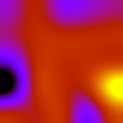
\includegraphics[interpolate=true,width=1.230000in,height=1.230000in]{graph/res/fisica_4sensores-img2.png}}%
\end{pgfscope}%
\begin{pgfscope}%
\pgfsetrectcap%
\pgfsetmiterjoin%
\pgfsetlinewidth{0.803000pt}%
\definecolor{currentstroke}{rgb}{0.000000,0.000000,0.000000}%
\pgfsetstrokecolor{currentstroke}%
\pgfsetdash{}{0pt}%
\pgfpathmoveto{\pgfqpoint{0.875000in}{0.813486in}}%
\pgfpathlineto{\pgfqpoint{0.875000in}{2.036514in}}%
\pgfusepath{stroke}%
\end{pgfscope}%
\begin{pgfscope}%
\pgfsetrectcap%
\pgfsetmiterjoin%
\pgfsetlinewidth{0.803000pt}%
\definecolor{currentstroke}{rgb}{0.000000,0.000000,0.000000}%
\pgfsetstrokecolor{currentstroke}%
\pgfsetdash{}{0pt}%
\pgfpathmoveto{\pgfqpoint{2.098027in}{0.813486in}}%
\pgfpathlineto{\pgfqpoint{2.098027in}{2.036514in}}%
\pgfusepath{stroke}%
\end{pgfscope}%
\begin{pgfscope}%
\pgfsetrectcap%
\pgfsetmiterjoin%
\pgfsetlinewidth{0.803000pt}%
\definecolor{currentstroke}{rgb}{0.000000,0.000000,0.000000}%
\pgfsetstrokecolor{currentstroke}%
\pgfsetdash{}{0pt}%
\pgfpathmoveto{\pgfqpoint{0.875000in}{0.813486in}}%
\pgfpathlineto{\pgfqpoint{2.098027in}{0.813486in}}%
\pgfusepath{stroke}%
\end{pgfscope}%
\begin{pgfscope}%
\pgfsetrectcap%
\pgfsetmiterjoin%
\pgfsetlinewidth{0.803000pt}%
\definecolor{currentstroke}{rgb}{0.000000,0.000000,0.000000}%
\pgfsetstrokecolor{currentstroke}%
\pgfsetdash{}{0pt}%
\pgfpathmoveto{\pgfqpoint{0.875000in}{2.036514in}}%
\pgfpathlineto{\pgfqpoint{2.098027in}{2.036514in}}%
\pgfusepath{stroke}%
\end{pgfscope}%
\begin{pgfscope}%
\pgfsys@transformshift{1.060264in}{0.995000in}%
\pgftext[left,bottom]{
\includegraphics[interpolate=true,width=0.860000in,height=0.860000in]{graph/res/fisica_4sensores-img3.png}}%
\end{pgfscope}%
\begin{pgfscope}%
\definecolor{textcolor}{rgb}{0.000000,0.000000,0.000000}%
\pgfsetstrokecolor{textcolor}%
\pgfsetfillcolor{textcolor}%
\pgftext[x=1.486514in,y=2.119847in,,base]{\color{textcolor}\rmfamily\fontsize{12.000000}{14.400000}\selectfont Error en eje $y$}%
\end{pgfscope}%
\begin{pgfscope}%
\pgfsetbuttcap%
\pgfsetmiterjoin%
\definecolor{currentfill}{rgb}{1.000000,1.000000,1.000000}%
\pgfsetfillcolor{currentfill}%
\pgfsetlinewidth{0.000000pt}%
\definecolor{currentstroke}{rgb}{0.000000,0.000000,0.000000}%
\pgfsetstrokecolor{currentstroke}%
\pgfsetstrokeopacity{0.000000}%
\pgfsetdash{}{0pt}%
\pgfpathmoveto{\pgfqpoint{2.805636in}{1.077254in}}%
\pgfpathlineto{\pgfqpoint{5.601127in}{1.077254in}}%
\pgfpathlineto{\pgfqpoint{5.601127in}{3.872746in}}%
\pgfpathlineto{\pgfqpoint{2.805636in}{3.872746in}}%
\pgfpathclose%
\pgfusepath{fill}%
\end{pgfscope}%
\begin{pgfscope}%
\pgfpathrectangle{\pgfqpoint{2.805636in}{1.077254in}}{\pgfqpoint{2.795491in}{2.795491in}}%
\pgfusepath{clip}%
\pgfsys@transformshift{2.805636in}{1.077254in}%
\pgftext[left,bottom]{
\includegraphics[interpolate=true,width=2.800000in,height=2.800000in]{graph/res/fisica_4sensores-img4.png}}%
\end{pgfscope}%
\begin{pgfscope}%
\pgfsetbuttcap%
\pgfsetroundjoin%
\definecolor{currentfill}{rgb}{0.000000,0.000000,0.000000}%
\pgfsetfillcolor{currentfill}%
\pgfsetlinewidth{0.803000pt}%
\definecolor{currentstroke}{rgb}{0.000000,0.000000,0.000000}%
\pgfsetstrokecolor{currentstroke}%
\pgfsetdash{}{0pt}%
\pgfsys@defobject{currentmarker}{\pgfqpoint{0.000000in}{-0.048611in}}{\pgfqpoint{0.000000in}{0.000000in}}{%
\pgfpathmoveto{\pgfqpoint{0.000000in}{0.000000in}}%
\pgfpathlineto{\pgfqpoint{0.000000in}{-0.048611in}}%
\pgfusepath{stroke,fill}%
}%
\begin{pgfscope}%
\pgfsys@transformshift{3.085185in}{1.077254in}%
\pgfsys@useobject{currentmarker}{}%
\end{pgfscope}%
\end{pgfscope}%
\begin{pgfscope}%
\definecolor{textcolor}{rgb}{0.000000,0.000000,0.000000}%
\pgfsetstrokecolor{textcolor}%
\pgfsetfillcolor{textcolor}%
\pgftext[x=3.085185in,y=0.980032in,,top]{\color{textcolor}\rmfamily\fontsize{10.000000}{12.000000}\selectfont 1.0}%
\end{pgfscope}%
\begin{pgfscope}%
\pgfsetbuttcap%
\pgfsetroundjoin%
\definecolor{currentfill}{rgb}{0.000000,0.000000,0.000000}%
\pgfsetfillcolor{currentfill}%
\pgfsetlinewidth{0.803000pt}%
\definecolor{currentstroke}{rgb}{0.000000,0.000000,0.000000}%
\pgfsetstrokecolor{currentstroke}%
\pgfsetdash{}{0pt}%
\pgfsys@defobject{currentmarker}{\pgfqpoint{0.000000in}{-0.048611in}}{\pgfqpoint{0.000000in}{0.000000in}}{%
\pgfpathmoveto{\pgfqpoint{0.000000in}{0.000000in}}%
\pgfpathlineto{\pgfqpoint{0.000000in}{-0.048611in}}%
\pgfusepath{stroke,fill}%
}%
\begin{pgfscope}%
\pgfsys@transformshift{3.644283in}{1.077254in}%
\pgfsys@useobject{currentmarker}{}%
\end{pgfscope}%
\end{pgfscope}%
\begin{pgfscope}%
\definecolor{textcolor}{rgb}{0.000000,0.000000,0.000000}%
\pgfsetstrokecolor{textcolor}%
\pgfsetfillcolor{textcolor}%
\pgftext[x=3.644283in,y=0.980032in,,top]{\color{textcolor}\rmfamily\fontsize{10.000000}{12.000000}\selectfont 3.25}%
\end{pgfscope}%
\begin{pgfscope}%
\pgfsetbuttcap%
\pgfsetroundjoin%
\definecolor{currentfill}{rgb}{0.000000,0.000000,0.000000}%
\pgfsetfillcolor{currentfill}%
\pgfsetlinewidth{0.803000pt}%
\definecolor{currentstroke}{rgb}{0.000000,0.000000,0.000000}%
\pgfsetstrokecolor{currentstroke}%
\pgfsetdash{}{0pt}%
\pgfsys@defobject{currentmarker}{\pgfqpoint{0.000000in}{-0.048611in}}{\pgfqpoint{0.000000in}{0.000000in}}{%
\pgfpathmoveto{\pgfqpoint{0.000000in}{0.000000in}}%
\pgfpathlineto{\pgfqpoint{0.000000in}{-0.048611in}}%
\pgfusepath{stroke,fill}%
}%
\begin{pgfscope}%
\pgfsys@transformshift{4.203382in}{1.077254in}%
\pgfsys@useobject{currentmarker}{}%
\end{pgfscope}%
\end{pgfscope}%
\begin{pgfscope}%
\definecolor{textcolor}{rgb}{0.000000,0.000000,0.000000}%
\pgfsetstrokecolor{textcolor}%
\pgfsetfillcolor{textcolor}%
\pgftext[x=4.203382in,y=0.980032in,,top]{\color{textcolor}\rmfamily\fontsize{10.000000}{12.000000}\selectfont 5.5}%
\end{pgfscope}%
\begin{pgfscope}%
\pgfsetbuttcap%
\pgfsetroundjoin%
\definecolor{currentfill}{rgb}{0.000000,0.000000,0.000000}%
\pgfsetfillcolor{currentfill}%
\pgfsetlinewidth{0.803000pt}%
\definecolor{currentstroke}{rgb}{0.000000,0.000000,0.000000}%
\pgfsetstrokecolor{currentstroke}%
\pgfsetdash{}{0pt}%
\pgfsys@defobject{currentmarker}{\pgfqpoint{0.000000in}{-0.048611in}}{\pgfqpoint{0.000000in}{0.000000in}}{%
\pgfpathmoveto{\pgfqpoint{0.000000in}{0.000000in}}%
\pgfpathlineto{\pgfqpoint{0.000000in}{-0.048611in}}%
\pgfusepath{stroke,fill}%
}%
\begin{pgfscope}%
\pgfsys@transformshift{4.762480in}{1.077254in}%
\pgfsys@useobject{currentmarker}{}%
\end{pgfscope}%
\end{pgfscope}%
\begin{pgfscope}%
\definecolor{textcolor}{rgb}{0.000000,0.000000,0.000000}%
\pgfsetstrokecolor{textcolor}%
\pgfsetfillcolor{textcolor}%
\pgftext[x=4.762480in,y=0.980032in,,top]{\color{textcolor}\rmfamily\fontsize{10.000000}{12.000000}\selectfont 7.75}%
\end{pgfscope}%
\begin{pgfscope}%
\pgfsetbuttcap%
\pgfsetroundjoin%
\definecolor{currentfill}{rgb}{0.000000,0.000000,0.000000}%
\pgfsetfillcolor{currentfill}%
\pgfsetlinewidth{0.803000pt}%
\definecolor{currentstroke}{rgb}{0.000000,0.000000,0.000000}%
\pgfsetstrokecolor{currentstroke}%
\pgfsetdash{}{0pt}%
\pgfsys@defobject{currentmarker}{\pgfqpoint{0.000000in}{-0.048611in}}{\pgfqpoint{0.000000in}{0.000000in}}{%
\pgfpathmoveto{\pgfqpoint{0.000000in}{0.000000in}}%
\pgfpathlineto{\pgfqpoint{0.000000in}{-0.048611in}}%
\pgfusepath{stroke,fill}%
}%
\begin{pgfscope}%
\pgfsys@transformshift{5.321578in}{1.077254in}%
\pgfsys@useobject{currentmarker}{}%
\end{pgfscope}%
\end{pgfscope}%
\begin{pgfscope}%
\definecolor{textcolor}{rgb}{0.000000,0.000000,0.000000}%
\pgfsetstrokecolor{textcolor}%
\pgfsetfillcolor{textcolor}%
\pgftext[x=5.321578in,y=0.980032in,,top]{\color{textcolor}\rmfamily\fontsize{10.000000}{12.000000}\selectfont 10.0}%
\end{pgfscope}%
\begin{pgfscope}%
\definecolor{textcolor}{rgb}{0.000000,0.000000,0.000000}%
\pgfsetstrokecolor{textcolor}%
\pgfsetfillcolor{textcolor}%
\pgftext[x=4.203382in,y=0.801822in,,top]{\color{textcolor}\rmfamily\fontsize{10.000000}{12.000000}\selectfont x [m]}%
\end{pgfscope}%
\begin{pgfscope}%
\pgfsetbuttcap%
\pgfsetroundjoin%
\definecolor{currentfill}{rgb}{0.000000,0.000000,0.000000}%
\pgfsetfillcolor{currentfill}%
\pgfsetlinewidth{0.803000pt}%
\definecolor{currentstroke}{rgb}{0.000000,0.000000,0.000000}%
\pgfsetstrokecolor{currentstroke}%
\pgfsetdash{}{0pt}%
\pgfsys@defobject{currentmarker}{\pgfqpoint{-0.048611in}{0.000000in}}{\pgfqpoint{-0.000000in}{0.000000in}}{%
\pgfpathmoveto{\pgfqpoint{-0.000000in}{0.000000in}}%
\pgfpathlineto{\pgfqpoint{-0.048611in}{0.000000in}}%
\pgfusepath{stroke,fill}%
}%
\begin{pgfscope}%
\pgfsys@transformshift{2.805636in}{1.356804in}%
\pgfsys@useobject{currentmarker}{}%
\end{pgfscope}%
\end{pgfscope}%
\begin{pgfscope}%
\definecolor{textcolor}{rgb}{0.000000,0.000000,0.000000}%
\pgfsetstrokecolor{textcolor}%
\pgfsetfillcolor{textcolor}%
\pgftext[x=2.530988in, y=1.308976in, left, base]{\color{textcolor}\rmfamily\fontsize{10.000000}{12.000000}\selectfont 1.0}%
\end{pgfscope}%
\begin{pgfscope}%
\pgfsetbuttcap%
\pgfsetroundjoin%
\definecolor{currentfill}{rgb}{0.000000,0.000000,0.000000}%
\pgfsetfillcolor{currentfill}%
\pgfsetlinewidth{0.803000pt}%
\definecolor{currentstroke}{rgb}{0.000000,0.000000,0.000000}%
\pgfsetstrokecolor{currentstroke}%
\pgfsetdash{}{0pt}%
\pgfsys@defobject{currentmarker}{\pgfqpoint{-0.048611in}{0.000000in}}{\pgfqpoint{-0.000000in}{0.000000in}}{%
\pgfpathmoveto{\pgfqpoint{-0.000000in}{0.000000in}}%
\pgfpathlineto{\pgfqpoint{-0.048611in}{0.000000in}}%
\pgfusepath{stroke,fill}%
}%
\begin{pgfscope}%
\pgfsys@transformshift{2.805636in}{1.915902in}%
\pgfsys@useobject{currentmarker}{}%
\end{pgfscope}%
\end{pgfscope}%
\begin{pgfscope}%
\definecolor{textcolor}{rgb}{0.000000,0.000000,0.000000}%
\pgfsetstrokecolor{textcolor}%
\pgfsetfillcolor{textcolor}%
\pgftext[x=2.461561in, y=1.868074in, left, base]{\color{textcolor}\rmfamily\fontsize{10.000000}{12.000000}\selectfont 3.25}%
\end{pgfscope}%
\begin{pgfscope}%
\pgfsetbuttcap%
\pgfsetroundjoin%
\definecolor{currentfill}{rgb}{0.000000,0.000000,0.000000}%
\pgfsetfillcolor{currentfill}%
\pgfsetlinewidth{0.803000pt}%
\definecolor{currentstroke}{rgb}{0.000000,0.000000,0.000000}%
\pgfsetstrokecolor{currentstroke}%
\pgfsetdash{}{0pt}%
\pgfsys@defobject{currentmarker}{\pgfqpoint{-0.048611in}{0.000000in}}{\pgfqpoint{-0.000000in}{0.000000in}}{%
\pgfpathmoveto{\pgfqpoint{-0.000000in}{0.000000in}}%
\pgfpathlineto{\pgfqpoint{-0.048611in}{0.000000in}}%
\pgfusepath{stroke,fill}%
}%
\begin{pgfscope}%
\pgfsys@transformshift{2.805636in}{2.475000in}%
\pgfsys@useobject{currentmarker}{}%
\end{pgfscope}%
\end{pgfscope}%
\begin{pgfscope}%
\definecolor{textcolor}{rgb}{0.000000,0.000000,0.000000}%
\pgfsetstrokecolor{textcolor}%
\pgfsetfillcolor{textcolor}%
\pgftext[x=2.530988in, y=2.427172in, left, base]{\color{textcolor}\rmfamily\fontsize{10.000000}{12.000000}\selectfont 5.5}%
\end{pgfscope}%
\begin{pgfscope}%
\pgfsetbuttcap%
\pgfsetroundjoin%
\definecolor{currentfill}{rgb}{0.000000,0.000000,0.000000}%
\pgfsetfillcolor{currentfill}%
\pgfsetlinewidth{0.803000pt}%
\definecolor{currentstroke}{rgb}{0.000000,0.000000,0.000000}%
\pgfsetstrokecolor{currentstroke}%
\pgfsetdash{}{0pt}%
\pgfsys@defobject{currentmarker}{\pgfqpoint{-0.048611in}{0.000000in}}{\pgfqpoint{-0.000000in}{0.000000in}}{%
\pgfpathmoveto{\pgfqpoint{-0.000000in}{0.000000in}}%
\pgfpathlineto{\pgfqpoint{-0.048611in}{0.000000in}}%
\pgfusepath{stroke,fill}%
}%
\begin{pgfscope}%
\pgfsys@transformshift{2.805636in}{3.034098in}%
\pgfsys@useobject{currentmarker}{}%
\end{pgfscope}%
\end{pgfscope}%
\begin{pgfscope}%
\definecolor{textcolor}{rgb}{0.000000,0.000000,0.000000}%
\pgfsetstrokecolor{textcolor}%
\pgfsetfillcolor{textcolor}%
\pgftext[x=2.461561in, y=2.986270in, left, base]{\color{textcolor}\rmfamily\fontsize{10.000000}{12.000000}\selectfont 7.75}%
\end{pgfscope}%
\begin{pgfscope}%
\pgfsetbuttcap%
\pgfsetroundjoin%
\definecolor{currentfill}{rgb}{0.000000,0.000000,0.000000}%
\pgfsetfillcolor{currentfill}%
\pgfsetlinewidth{0.803000pt}%
\definecolor{currentstroke}{rgb}{0.000000,0.000000,0.000000}%
\pgfsetstrokecolor{currentstroke}%
\pgfsetdash{}{0pt}%
\pgfsys@defobject{currentmarker}{\pgfqpoint{-0.048611in}{0.000000in}}{\pgfqpoint{-0.000000in}{0.000000in}}{%
\pgfpathmoveto{\pgfqpoint{-0.000000in}{0.000000in}}%
\pgfpathlineto{\pgfqpoint{-0.048611in}{0.000000in}}%
\pgfusepath{stroke,fill}%
}%
\begin{pgfscope}%
\pgfsys@transformshift{2.805636in}{3.593196in}%
\pgfsys@useobject{currentmarker}{}%
\end{pgfscope}%
\end{pgfscope}%
\begin{pgfscope}%
\definecolor{textcolor}{rgb}{0.000000,0.000000,0.000000}%
\pgfsetstrokecolor{textcolor}%
\pgfsetfillcolor{textcolor}%
\pgftext[x=2.461561in, y=3.545369in, left, base]{\color{textcolor}\rmfamily\fontsize{10.000000}{12.000000}\selectfont 10.0}%
\end{pgfscope}%
\begin{pgfscope}%
\definecolor{textcolor}{rgb}{0.000000,0.000000,0.000000}%
\pgfsetstrokecolor{textcolor}%
\pgfsetfillcolor{textcolor}%
\pgftext[x=2.406005in,y=2.475000in,,bottom,rotate=90.000000]{\color{textcolor}\rmfamily\fontsize{10.000000}{12.000000}\selectfont y [m]}%
\end{pgfscope}%
\begin{pgfscope}%
\pgfsetrectcap%
\pgfsetmiterjoin%
\pgfsetlinewidth{0.803000pt}%
\definecolor{currentstroke}{rgb}{0.000000,0.000000,0.000000}%
\pgfsetstrokecolor{currentstroke}%
\pgfsetdash{}{0pt}%
\pgfpathmoveto{\pgfqpoint{2.805636in}{1.077254in}}%
\pgfpathlineto{\pgfqpoint{2.805636in}{3.872746in}}%
\pgfusepath{stroke}%
\end{pgfscope}%
\begin{pgfscope}%
\pgfsetrectcap%
\pgfsetmiterjoin%
\pgfsetlinewidth{0.803000pt}%
\definecolor{currentstroke}{rgb}{0.000000,0.000000,0.000000}%
\pgfsetstrokecolor{currentstroke}%
\pgfsetdash{}{0pt}%
\pgfpathmoveto{\pgfqpoint{5.601127in}{1.077254in}}%
\pgfpathlineto{\pgfqpoint{5.601127in}{3.872746in}}%
\pgfusepath{stroke}%
\end{pgfscope}%
\begin{pgfscope}%
\pgfsetrectcap%
\pgfsetmiterjoin%
\pgfsetlinewidth{0.803000pt}%
\definecolor{currentstroke}{rgb}{0.000000,0.000000,0.000000}%
\pgfsetstrokecolor{currentstroke}%
\pgfsetdash{}{0pt}%
\pgfpathmoveto{\pgfqpoint{2.805636in}{1.077254in}}%
\pgfpathlineto{\pgfqpoint{5.601127in}{1.077254in}}%
\pgfusepath{stroke}%
\end{pgfscope}%
\begin{pgfscope}%
\pgfsetrectcap%
\pgfsetmiterjoin%
\pgfsetlinewidth{0.803000pt}%
\definecolor{currentstroke}{rgb}{0.000000,0.000000,0.000000}%
\pgfsetstrokecolor{currentstroke}%
\pgfsetdash{}{0pt}%
\pgfpathmoveto{\pgfqpoint{2.805636in}{3.872746in}}%
\pgfpathlineto{\pgfqpoint{5.601127in}{3.872746in}}%
\pgfusepath{stroke}%
\end{pgfscope}%
\begin{pgfscope}%
\definecolor{textcolor}{rgb}{1.000000,1.000000,1.000000}%
\pgfsetstrokecolor{textcolor}%
\pgfsetfillcolor{textcolor}%
\pgftext[x=2.927045in, y=1.402317in, left, base]{\color{textcolor}\rmfamily\fontsize{10.000000}{12.000000}\selectfont 24.46}%
\end{pgfscope}%
\begin{pgfscope}%
\definecolor{textcolor}{rgb}{1.000000,1.000000,1.000000}%
\pgfsetstrokecolor{textcolor}%
\pgfsetfillcolor{textcolor}%
\pgftext[x=2.907759in, y=1.250348in, left, base]{\color{textcolor}\rmfamily\fontsize{10.000000}{12.000000}\selectfont  (8.76)}%
\end{pgfscope}%
\begin{pgfscope}%
\definecolor{textcolor}{rgb}{1.000000,1.000000,1.000000}%
\pgfsetstrokecolor{textcolor}%
\pgfsetfillcolor{textcolor}%
\pgftext[x=3.486143in, y=1.402317in, left, base]{\color{textcolor}\rmfamily\fontsize{10.000000}{12.000000}\selectfont 20.69}%
\end{pgfscope}%
\begin{pgfscope}%
\definecolor{textcolor}{rgb}{1.000000,1.000000,1.000000}%
\pgfsetstrokecolor{textcolor}%
\pgfsetfillcolor{textcolor}%
\pgftext[x=3.432144in, y=1.250348in, left, base]{\color{textcolor}\rmfamily\fontsize{10.000000}{12.000000}\selectfont  (12.71)}%
\end{pgfscope}%
\begin{pgfscope}%
\definecolor{textcolor}{rgb}{1.000000,1.000000,1.000000}%
\pgfsetstrokecolor{textcolor}%
\pgfsetfillcolor{textcolor}%
\pgftext[x=4.079955in, y=1.402317in, left, base]{\color{textcolor}\rmfamily\fontsize{10.000000}{12.000000}\selectfont 5.54}%
\end{pgfscope}%
\begin{pgfscope}%
\definecolor{textcolor}{rgb}{1.000000,1.000000,1.000000}%
\pgfsetstrokecolor{textcolor}%
\pgfsetfillcolor{textcolor}%
\pgftext[x=4.025956in, y=1.250348in, left, base]{\color{textcolor}\rmfamily\fontsize{10.000000}{12.000000}\selectfont  (3.51)}%
\end{pgfscope}%
\begin{pgfscope}%
\definecolor{textcolor}{rgb}{1.000000,1.000000,1.000000}%
\pgfsetstrokecolor{textcolor}%
\pgfsetfillcolor{textcolor}%
\pgftext[x=4.604339in, y=1.402317in, left, base]{\color{textcolor}\rmfamily\fontsize{10.000000}{12.000000}\selectfont 37.33}%
\end{pgfscope}%
\begin{pgfscope}%
\definecolor{textcolor}{rgb}{1.000000,1.000000,1.000000}%
\pgfsetstrokecolor{textcolor}%
\pgfsetfillcolor{textcolor}%
\pgftext[x=4.550340in, y=1.250348in, left, base]{\color{textcolor}\rmfamily\fontsize{10.000000}{12.000000}\selectfont  (18.05)}%
\end{pgfscope}%
\begin{pgfscope}%
\definecolor{textcolor}{rgb}{1.000000,1.000000,1.000000}%
\pgfsetstrokecolor{textcolor}%
\pgfsetfillcolor{textcolor}%
\pgftext[x=5.163438in, y=1.402317in, left, base]{\color{textcolor}\rmfamily\fontsize{10.000000}{12.000000}\selectfont 27.83}%
\end{pgfscope}%
\begin{pgfscope}%
\definecolor{textcolor}{rgb}{1.000000,1.000000,1.000000}%
\pgfsetstrokecolor{textcolor}%
\pgfsetfillcolor{textcolor}%
\pgftext[x=5.109439in, y=1.250348in, left, base]{\color{textcolor}\rmfamily\fontsize{10.000000}{12.000000}\selectfont  (11.26)}%
\end{pgfscope}%
\begin{pgfscope}%
\definecolor{textcolor}{rgb}{1.000000,1.000000,1.000000}%
\pgfsetstrokecolor{textcolor}%
\pgfsetfillcolor{textcolor}%
\pgftext[x=2.927045in, y=1.961415in, left, base]{\color{black}\rmfamily\fontsize{10.000000}{12.000000}\selectfont 52.38}%
\end{pgfscope}%
\begin{pgfscope}%
\definecolor{textcolor}{rgb}{1.000000,1.000000,1.000000}%
\pgfsetstrokecolor{textcolor}%
\pgfsetfillcolor{textcolor}%
\pgftext[x=2.873046in, y=1.809446in, left, base]{\color{black}\rmfamily\fontsize{10.000000}{12.000000}\selectfont  (10.92)}%
\end{pgfscope}%
\begin{pgfscope}%
\definecolor{textcolor}{rgb}{1.000000,1.000000,1.000000}%
\pgfsetstrokecolor{textcolor}%
\pgfsetfillcolor{textcolor}%
\pgftext[x=3.555570in, y=1.961415in, left, base]{\color{textcolor}\rmfamily\fontsize{10.000000}{12.000000}\selectfont 0.0}%
\end{pgfscope}%
\begin{pgfscope}%
\definecolor{textcolor}{rgb}{1.000000,1.000000,1.000000}%
\pgfsetstrokecolor{textcolor}%
\pgfsetfillcolor{textcolor}%
\pgftext[x=3.501571in, y=1.809446in, left, base]{\color{textcolor}\rmfamily\fontsize{10.000000}{12.000000}\selectfont  (0.0)}%
\end{pgfscope}%
\begin{pgfscope}%
\definecolor{textcolor}{rgb}{1.000000,1.000000,1.000000}%
\pgfsetstrokecolor{textcolor}%
\pgfsetfillcolor{textcolor}%
\pgftext[x=4.114669in, y=1.961415in, left, base]{\color{textcolor}\rmfamily\fontsize{10.000000}{12.000000}\selectfont 0.0}%
\end{pgfscope}%
\begin{pgfscope}%
\definecolor{textcolor}{rgb}{1.000000,1.000000,1.000000}%
\pgfsetstrokecolor{textcolor}%
\pgfsetfillcolor{textcolor}%
\pgftext[x=4.060670in, y=1.809446in, left, base]{\color{textcolor}\rmfamily\fontsize{10.000000}{12.000000}\selectfont  (0.0)}%
\end{pgfscope}%
\begin{pgfscope}%
\definecolor{textcolor}{rgb}{1.000000,1.000000,1.000000}%
\pgfsetstrokecolor{textcolor}%
\pgfsetfillcolor{textcolor}%
\pgftext[x=4.673767in, y=1.961415in, left, base]{\color{textcolor}\rmfamily\fontsize{10.000000}{12.000000}\selectfont 0.0}%
\end{pgfscope}%
\begin{pgfscope}%
\definecolor{textcolor}{rgb}{1.000000,1.000000,1.000000}%
\pgfsetstrokecolor{textcolor}%
\pgfsetfillcolor{textcolor}%
\pgftext[x=4.619768in, y=1.809446in, left, base]{\color{textcolor}\rmfamily\fontsize{10.000000}{12.000000}\selectfont  (0.0)}%
\end{pgfscope}%
\begin{pgfscope}%
\definecolor{textcolor}{rgb}{1.000000,1.000000,1.000000}%
\pgfsetstrokecolor{textcolor}%
\pgfsetfillcolor{textcolor}%
\pgftext[x=5.163438in, y=1.961415in, left, base]{\color{textcolor}\rmfamily\fontsize{10.000000}{12.000000}\selectfont 41.55}%
\end{pgfscope}%
\begin{pgfscope}%
\definecolor{textcolor}{rgb}{1.000000,1.000000,1.000000}%
\pgfsetstrokecolor{textcolor}%
\pgfsetfillcolor{textcolor}%
\pgftext[x=5.144152in, y=1.809446in, left, base]{\color{textcolor}\rmfamily\fontsize{10.000000}{12.000000}\selectfont  (8.39)}%
\end{pgfscope}%
\begin{pgfscope}%
\definecolor{textcolor}{rgb}{1.000000,1.000000,1.000000}%
\pgfsetstrokecolor{textcolor}%
\pgfsetfillcolor{textcolor}%
\pgftext[x=2.961759in, y=2.520514in, left, base]{\color{textcolor}\rmfamily\fontsize{10.000000}{12.000000}\selectfont 30.8}%
\end{pgfscope}%
\begin{pgfscope}%
\definecolor{textcolor}{rgb}{1.000000,1.000000,1.000000}%
\pgfsetstrokecolor{textcolor}%
\pgfsetfillcolor{textcolor}%
\pgftext[x=2.907759in, y=2.368545in, left, base]{\color{textcolor}\rmfamily\fontsize{10.000000}{12.000000}\selectfont  (0.33)}%
\end{pgfscope}%
\begin{pgfscope}%
\definecolor{textcolor}{rgb}{1.000000,1.000000,1.000000}%
\pgfsetstrokecolor{textcolor}%
\pgfsetfillcolor{textcolor}%
\pgftext[x=3.555570in, y=2.520514in, left, base]{\color{textcolor}\rmfamily\fontsize{10.000000}{12.000000}\selectfont 0.0}%
\end{pgfscope}%
\begin{pgfscope}%
\definecolor{textcolor}{rgb}{1.000000,1.000000,1.000000}%
\pgfsetstrokecolor{textcolor}%
\pgfsetfillcolor{textcolor}%
\pgftext[x=3.501571in, y=2.368545in, left, base]{\color{textcolor}\rmfamily\fontsize{10.000000}{12.000000}\selectfont  (0.0)}%
\end{pgfscope}%
\begin{pgfscope}%
\definecolor{textcolor}{rgb}{1.000000,1.000000,1.000000}%
\pgfsetstrokecolor{textcolor}%
\pgfsetfillcolor{textcolor}%
\pgftext[x=4.114669in, y=2.520514in, left, base]{\color{textcolor}\rmfamily\fontsize{10.000000}{12.000000}\selectfont 0.0}%
\end{pgfscope}%
\begin{pgfscope}%
\definecolor{textcolor}{rgb}{1.000000,1.000000,1.000000}%
\pgfsetstrokecolor{textcolor}%
\pgfsetfillcolor{textcolor}%
\pgftext[x=4.060670in, y=2.368545in, left, base]{\color{textcolor}\rmfamily\fontsize{10.000000}{12.000000}\selectfont  (0.0)}%
\end{pgfscope}%
\begin{pgfscope}%
\definecolor{textcolor}{rgb}{1.000000,1.000000,1.000000}%
\pgfsetstrokecolor{textcolor}%
\pgfsetfillcolor{textcolor}%
\pgftext[x=4.673767in, y=2.520514in, left, base]{\color{textcolor}\rmfamily\fontsize{10.000000}{12.000000}\selectfont 0.0}%
\end{pgfscope}%
\begin{pgfscope}%
\definecolor{textcolor}{rgb}{1.000000,1.000000,1.000000}%
\pgfsetstrokecolor{textcolor}%
\pgfsetfillcolor{textcolor}%
\pgftext[x=4.619768in, y=2.368545in, left, base]{\color{textcolor}\rmfamily\fontsize{10.000000}{12.000000}\selectfont  (0.0)}%
\end{pgfscope}%
\begin{pgfscope}%
\definecolor{textcolor}{rgb}{1.000000,1.000000,1.000000}%
\pgfsetstrokecolor{textcolor}%
\pgfsetfillcolor{textcolor}%
\pgftext[x=5.163438in, y=2.520514in, left, base]{\color{textcolor}\rmfamily\fontsize{10.000000}{12.000000}\selectfont 14.19}%
\end{pgfscope}%
\begin{pgfscope}%
\definecolor{textcolor}{rgb}{1.000000,1.000000,1.000000}%
\pgfsetstrokecolor{textcolor}%
\pgfsetfillcolor{textcolor}%
\pgftext[x=5.144152in, y=2.368545in, left, base]{\color{textcolor}\rmfamily\fontsize{10.000000}{12.000000}\selectfont  (0.85)}%
\end{pgfscope}%
\begin{pgfscope}%
\definecolor{textcolor}{rgb}{1.000000,1.000000,1.000000}%
\pgfsetstrokecolor{textcolor}%
\pgfsetfillcolor{textcolor}%
\pgftext[x=2.927045in, y=3.079612in, left, base]{\color{textcolor}\rmfamily\fontsize{10.000000}{12.000000}\selectfont 12.32}%
\end{pgfscope}%
\begin{pgfscope}%
\definecolor{textcolor}{rgb}{1.000000,1.000000,1.000000}%
\pgfsetstrokecolor{textcolor}%
\pgfsetfillcolor{textcolor}%
\pgftext[x=2.907759in, y=2.927643in, left, base]{\color{textcolor}\rmfamily\fontsize{10.000000}{12.000000}\selectfont  (6.52)}%
\end{pgfscope}%
\begin{pgfscope}%
\definecolor{textcolor}{rgb}{1.000000,1.000000,1.000000}%
\pgfsetstrokecolor{textcolor}%
\pgfsetfillcolor{textcolor}%
\pgftext[x=3.555570in, y=3.079612in, left, base]{\color{textcolor}\rmfamily\fontsize{10.000000}{12.000000}\selectfont 0.0}%
\end{pgfscope}%
\begin{pgfscope}%
\definecolor{textcolor}{rgb}{1.000000,1.000000,1.000000}%
\pgfsetstrokecolor{textcolor}%
\pgfsetfillcolor{textcolor}%
\pgftext[x=3.501571in, y=2.927643in, left, base]{\color{textcolor}\rmfamily\fontsize{10.000000}{12.000000}\selectfont  (0.0)}%
\end{pgfscope}%
\begin{pgfscope}%
\definecolor{textcolor}{rgb}{1.000000,1.000000,1.000000}%
\pgfsetstrokecolor{textcolor}%
\pgfsetfillcolor{textcolor}%
\pgftext[x=4.114669in, y=3.079612in, left, base]{\color{textcolor}\rmfamily\fontsize{10.000000}{12.000000}\selectfont 0.0}%
\end{pgfscope}%
\begin{pgfscope}%
\definecolor{textcolor}{rgb}{1.000000,1.000000,1.000000}%
\pgfsetstrokecolor{textcolor}%
\pgfsetfillcolor{textcolor}%
\pgftext[x=4.060670in, y=2.927643in, left, base]{\color{textcolor}\rmfamily\fontsize{10.000000}{12.000000}\selectfont  (0.0)}%
\end{pgfscope}%
\begin{pgfscope}%
\definecolor{textcolor}{rgb}{1.000000,1.000000,1.000000}%
\pgfsetstrokecolor{textcolor}%
\pgfsetfillcolor{textcolor}%
\pgftext[x=4.673767in, y=3.079612in, left, base]{\color{textcolor}\rmfamily\fontsize{10.000000}{12.000000}\selectfont 0.0}%
\end{pgfscope}%
\begin{pgfscope}%
\definecolor{textcolor}{rgb}{1.000000,1.000000,1.000000}%
\pgfsetstrokecolor{textcolor}%
\pgfsetfillcolor{textcolor}%
\pgftext[x=4.619768in, y=2.927643in, left, base]{\color{textcolor}\rmfamily\fontsize{10.000000}{12.000000}\selectfont  (0.0)}%
\end{pgfscope}%
\begin{pgfscope}%
\definecolor{textcolor}{rgb}{1.000000,1.000000,1.000000}%
\pgfsetstrokecolor{textcolor}%
\pgfsetfillcolor{textcolor}%
\pgftext[x=5.163438in, y=3.079612in, left, base]{\color{textcolor}\rmfamily\fontsize{10.000000}{12.000000}\selectfont 21.08}%
\end{pgfscope}%
\begin{pgfscope}%
\definecolor{textcolor}{rgb}{1.000000,1.000000,1.000000}%
\pgfsetstrokecolor{textcolor}%
\pgfsetfillcolor{textcolor}%
\pgftext[x=5.178866in, y=2.927643in, left, base]{\color{textcolor}\rmfamily\fontsize{10.000000}{12.000000}\selectfont  (3.4)}%
\end{pgfscope}%
\begin{pgfscope}%
\definecolor{textcolor}{rgb}{1.000000,1.000000,1.000000}%
\pgfsetstrokecolor{textcolor}%
\pgfsetfillcolor{textcolor}%
\pgftext[x=2.927045in, y=3.638710in, left, base]{\color{textcolor}\rmfamily\fontsize{10.000000}{12.000000}\selectfont 14.62}%
\end{pgfscope}%
\begin{pgfscope}%
\definecolor{textcolor}{rgb}{1.000000,1.000000,1.000000}%
\pgfsetstrokecolor{textcolor}%
\pgfsetfillcolor{textcolor}%
\pgftext[x=2.907759in, y=3.486741in, left, base]{\color{textcolor}\rmfamily\fontsize{10.000000}{12.000000}\selectfont  (3.06)}%
\end{pgfscope}%
\begin{pgfscope}%
\definecolor{textcolor}{rgb}{1.000000,1.000000,1.000000}%
\pgfsetstrokecolor{textcolor}%
\pgfsetfillcolor{textcolor}%
\pgftext[x=3.486143in, y=3.638710in, left, base]{\color{textcolor}\rmfamily\fontsize{10.000000}{12.000000}\selectfont 14.23}%
\end{pgfscope}%
\begin{pgfscope}%
\definecolor{textcolor}{rgb}{1.000000,1.000000,1.000000}%
\pgfsetstrokecolor{textcolor}%
\pgfsetfillcolor{textcolor}%
\pgftext[x=3.466858in, y=3.486741in, left, base]{\color{textcolor}\rmfamily\fontsize{10.000000}{12.000000}\selectfont  (9.05)}%
\end{pgfscope}%
\begin{pgfscope}%
\definecolor{textcolor}{rgb}{1.000000,1.000000,1.000000}%
\pgfsetstrokecolor{textcolor}%
\pgfsetfillcolor{textcolor}%
\pgftext[x=4.079955in, y=3.638710in, left, base]{\color{textcolor}\rmfamily\fontsize{10.000000}{12.000000}\selectfont 27.4}%
\end{pgfscope}%
\begin{pgfscope}%
\definecolor{textcolor}{rgb}{1.000000,1.000000,1.000000}%
\pgfsetstrokecolor{textcolor}%
\pgfsetfillcolor{textcolor}%
\pgftext[x=4.025956in, y=3.486741in, left, base]{\color{textcolor}\rmfamily\fontsize{10.000000}{12.000000}\selectfont  (1.15)}%
\end{pgfscope}%
\begin{pgfscope}%
\definecolor{textcolor}{rgb}{1.000000,1.000000,1.000000}%
\pgfsetstrokecolor{textcolor}%
\pgfsetfillcolor{textcolor}%
\pgftext[x=4.604339in, y=3.638710in, left, base]{\color{black}\rmfamily\fontsize{10.000000}{12.000000}\selectfont 44.59}%
\end{pgfscope}%
\begin{pgfscope}%
\definecolor{textcolor}{rgb}{1.000000,1.000000,1.000000}%
\pgfsetstrokecolor{textcolor}%
\pgfsetfillcolor{textcolor}%
\pgftext[x=4.585054in, y=3.486741in, left, base]{\color{black}\rmfamily\fontsize{10.000000}{12.000000}\selectfont  (4.25)}%
\end{pgfscope}%
\begin{pgfscope}%
\definecolor{textcolor}{rgb}{1.000000,1.000000,1.000000}%
\pgfsetstrokecolor{textcolor}%
\pgfsetfillcolor{textcolor}%
\pgftext[x=5.163438in, y=3.638710in, left, base]{\color{textcolor}\rmfamily\fontsize{10.000000}{12.000000}\selectfont 28.77}%
\end{pgfscope}%
\begin{pgfscope}%
\definecolor{textcolor}{rgb}{1.000000,1.000000,1.000000}%
\pgfsetstrokecolor{textcolor}%
\pgfsetfillcolor{textcolor}%
\pgftext[x=5.109439in, y=3.486741in, left, base]{\color{textcolor}\rmfamily\fontsize{10.000000}{12.000000}\selectfont  (13.24)}%
\end{pgfscope}%
\begin{pgfscope}%
\pgfsys@transformshift{3.350882in}{1.615000in}%
\pgftext[left,bottom]{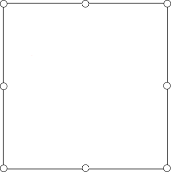
\includegraphics[interpolate=true,width=1.710000in,height=1.720000in]{graph/res/fisica_4sensores-img5.png}}%
\end{pgfscope}%
\begin{pgfscope}%
\definecolor{textcolor}{rgb}{0.000000,0.000000,0.000000}%
\pgfsetstrokecolor{textcolor}%
\pgfsetfillcolor{textcolor}%
\pgftext[x=4.203382in,y=3.956079in,,base]{\color{textcolor}\rmfamily\fontsize{12.000000}{14.400000}\selectfont Error en posición [cm]}%
\end{pgfscope}%
\begin{pgfscope}%
\pgfpathrectangle{\pgfqpoint{5.775845in}{1.127500in}}{\pgfqpoint{0.134750in}{2.695000in}}%
\pgfusepath{clip}%
\pgfsetbuttcap%
\pgfsetmiterjoin%
\definecolor{currentfill}{rgb}{1.000000,1.000000,1.000000}%
\pgfsetfillcolor{currentfill}%
\pgfsetlinewidth{0.010037pt}%
\definecolor{currentstroke}{rgb}{1.000000,1.000000,1.000000}%
\pgfsetstrokecolor{currentstroke}%
\pgfsetdash{}{0pt}%
\pgfpathmoveto{\pgfqpoint{5.775845in}{1.127500in}}%
\pgfpathlineto{\pgfqpoint{5.775845in}{1.138027in}}%
\pgfpathlineto{\pgfqpoint{5.775845in}{3.811973in}}%
\pgfpathlineto{\pgfqpoint{5.775845in}{3.822500in}}%
\pgfpathlineto{\pgfqpoint{5.910595in}{3.822500in}}%
\pgfpathlineto{\pgfqpoint{5.910595in}{3.811973in}}%
\pgfpathlineto{\pgfqpoint{5.910595in}{1.138027in}}%
\pgfpathlineto{\pgfqpoint{5.910595in}{1.127500in}}%
\pgfpathclose%
\pgfusepath{stroke,fill}%
\end{pgfscope}%
\begin{pgfscope}%
\pgfsys@transformshift{5.780000in}{1.130000in}%
\pgftext[left,bottom]{
\includegraphics[interpolate=true,width=0.130000in,height=2.690000in]{graph/res/fisica_4sensores-img6.png}}%
\end{pgfscope}%
\begin{pgfscope}%
\pgfsetbuttcap%
\pgfsetroundjoin%
\definecolor{currentfill}{rgb}{0.000000,0.000000,0.000000}%
\pgfsetfillcolor{currentfill}%
\pgfsetlinewidth{0.803000pt}%
\definecolor{currentstroke}{rgb}{0.000000,0.000000,0.000000}%
\pgfsetstrokecolor{currentstroke}%
\pgfsetdash{}{0pt}%
\pgfsys@defobject{currentmarker}{\pgfqpoint{0.000000in}{0.000000in}}{\pgfqpoint{0.048611in}{0.000000in}}{%
\pgfpathmoveto{\pgfqpoint{0.000000in}{0.000000in}}%
\pgfpathlineto{\pgfqpoint{0.048611in}{0.000000in}}%
\pgfusepath{stroke,fill}%
}%
\begin{pgfscope}%
\pgfsys@transformshift{5.910595in}{1.127500in}%
\pgfsys@useobject{currentmarker}{}%
\end{pgfscope}%
\end{pgfscope}%
\begin{pgfscope}%
\definecolor{textcolor}{rgb}{0.000000,0.000000,0.000000}%
\pgfsetstrokecolor{textcolor}%
\pgfsetfillcolor{textcolor}%
\pgftext[x=6.007818in, y=1.079672in, left, base]{\color{textcolor}\rmfamily\fontsize{10.000000}{12.000000}\selectfont \(\displaystyle {0}\)}%
\end{pgfscope}%
\begin{pgfscope}%
\pgfsetbuttcap%
\pgfsetroundjoin%
\definecolor{currentfill}{rgb}{0.000000,0.000000,0.000000}%
\pgfsetfillcolor{currentfill}%
\pgfsetlinewidth{0.803000pt}%
\definecolor{currentstroke}{rgb}{0.000000,0.000000,0.000000}%
\pgfsetstrokecolor{currentstroke}%
\pgfsetdash{}{0pt}%
\pgfsys@defobject{currentmarker}{\pgfqpoint{0.000000in}{0.000000in}}{\pgfqpoint{0.048611in}{0.000000in}}{%
\pgfpathmoveto{\pgfqpoint{0.000000in}{0.000000in}}%
\pgfpathlineto{\pgfqpoint{0.048611in}{0.000000in}}%
\pgfusepath{stroke,fill}%
}%
\begin{pgfscope}%
\pgfsys@transformshift{5.910595in}{1.641990in}%
\pgfsys@useobject{currentmarker}{}%
\end{pgfscope}%
\end{pgfscope}%
\begin{pgfscope}%
\definecolor{textcolor}{rgb}{0.000000,0.000000,0.000000}%
\pgfsetstrokecolor{textcolor}%
\pgfsetfillcolor{textcolor}%
\pgftext[x=6.007818in, y=1.594162in, left, base]{\color{textcolor}\rmfamily\fontsize{10.000000}{12.000000}\selectfont \(\displaystyle {10}\)}%
\end{pgfscope}%
\begin{pgfscope}%
\pgfsetbuttcap%
\pgfsetroundjoin%
\definecolor{currentfill}{rgb}{0.000000,0.000000,0.000000}%
\pgfsetfillcolor{currentfill}%
\pgfsetlinewidth{0.803000pt}%
\definecolor{currentstroke}{rgb}{0.000000,0.000000,0.000000}%
\pgfsetstrokecolor{currentstroke}%
\pgfsetdash{}{0pt}%
\pgfsys@defobject{currentmarker}{\pgfqpoint{0.000000in}{0.000000in}}{\pgfqpoint{0.048611in}{0.000000in}}{%
\pgfpathmoveto{\pgfqpoint{0.000000in}{0.000000in}}%
\pgfpathlineto{\pgfqpoint{0.048611in}{0.000000in}}%
\pgfusepath{stroke,fill}%
}%
\begin{pgfscope}%
\pgfsys@transformshift{5.910595in}{2.156480in}%
\pgfsys@useobject{currentmarker}{}%
\end{pgfscope}%
\end{pgfscope}%
\begin{pgfscope}%
\definecolor{textcolor}{rgb}{0.000000,0.000000,0.000000}%
\pgfsetstrokecolor{textcolor}%
\pgfsetfillcolor{textcolor}%
\pgftext[x=6.007818in, y=2.108653in, left, base]{\color{textcolor}\rmfamily\fontsize{10.000000}{12.000000}\selectfont \(\displaystyle {20}\)}%
\end{pgfscope}%
\begin{pgfscope}%
\pgfsetbuttcap%
\pgfsetroundjoin%
\definecolor{currentfill}{rgb}{0.000000,0.000000,0.000000}%
\pgfsetfillcolor{currentfill}%
\pgfsetlinewidth{0.803000pt}%
\definecolor{currentstroke}{rgb}{0.000000,0.000000,0.000000}%
\pgfsetstrokecolor{currentstroke}%
\pgfsetdash{}{0pt}%
\pgfsys@defobject{currentmarker}{\pgfqpoint{0.000000in}{0.000000in}}{\pgfqpoint{0.048611in}{0.000000in}}{%
\pgfpathmoveto{\pgfqpoint{0.000000in}{0.000000in}}%
\pgfpathlineto{\pgfqpoint{0.048611in}{0.000000in}}%
\pgfusepath{stroke,fill}%
}%
\begin{pgfscope}%
\pgfsys@transformshift{5.910595in}{2.670971in}%
\pgfsys@useobject{currentmarker}{}%
\end{pgfscope}%
\end{pgfscope}%
\begin{pgfscope}%
\definecolor{textcolor}{rgb}{0.000000,0.000000,0.000000}%
\pgfsetstrokecolor{textcolor}%
\pgfsetfillcolor{textcolor}%
\pgftext[x=6.007818in, y=2.623143in, left, base]{\color{textcolor}\rmfamily\fontsize{10.000000}{12.000000}\selectfont \(\displaystyle {30}\)}%
\end{pgfscope}%
\begin{pgfscope}%
\pgfsetbuttcap%
\pgfsetroundjoin%
\definecolor{currentfill}{rgb}{0.000000,0.000000,0.000000}%
\pgfsetfillcolor{currentfill}%
\pgfsetlinewidth{0.803000pt}%
\definecolor{currentstroke}{rgb}{0.000000,0.000000,0.000000}%
\pgfsetstrokecolor{currentstroke}%
\pgfsetdash{}{0pt}%
\pgfsys@defobject{currentmarker}{\pgfqpoint{0.000000in}{0.000000in}}{\pgfqpoint{0.048611in}{0.000000in}}{%
\pgfpathmoveto{\pgfqpoint{0.000000in}{0.000000in}}%
\pgfpathlineto{\pgfqpoint{0.048611in}{0.000000in}}%
\pgfusepath{stroke,fill}%
}%
\begin{pgfscope}%
\pgfsys@transformshift{5.910595in}{3.185461in}%
\pgfsys@useobject{currentmarker}{}%
\end{pgfscope}%
\end{pgfscope}%
\begin{pgfscope}%
\definecolor{textcolor}{rgb}{0.000000,0.000000,0.000000}%
\pgfsetstrokecolor{textcolor}%
\pgfsetfillcolor{textcolor}%
\pgftext[x=6.007818in, y=3.137633in, left, base]{\color{textcolor}\rmfamily\fontsize{10.000000}{12.000000}\selectfont \(\displaystyle {40}\)}%
\end{pgfscope}%
\begin{pgfscope}%
\pgfsetbuttcap%
\pgfsetroundjoin%
\definecolor{currentfill}{rgb}{0.000000,0.000000,0.000000}%
\pgfsetfillcolor{currentfill}%
\pgfsetlinewidth{0.803000pt}%
\definecolor{currentstroke}{rgb}{0.000000,0.000000,0.000000}%
\pgfsetstrokecolor{currentstroke}%
\pgfsetdash{}{0pt}%
\pgfsys@defobject{currentmarker}{\pgfqpoint{0.000000in}{0.000000in}}{\pgfqpoint{0.048611in}{0.000000in}}{%
\pgfpathmoveto{\pgfqpoint{0.000000in}{0.000000in}}%
\pgfpathlineto{\pgfqpoint{0.048611in}{0.000000in}}%
\pgfusepath{stroke,fill}%
}%
\begin{pgfscope}%
\pgfsys@transformshift{5.910595in}{3.699951in}%
\pgfsys@useobject{currentmarker}{}%
\end{pgfscope}%
\end{pgfscope}%
\begin{pgfscope}%
\definecolor{textcolor}{rgb}{0.000000,0.000000,0.000000}%
\pgfsetstrokecolor{textcolor}%
\pgfsetfillcolor{textcolor}%
\pgftext[x=6.007818in, y=3.652123in, left, base]{\color{textcolor}\rmfamily\fontsize{10.000000}{12.000000}\selectfont \(\displaystyle {50}\)}%
\end{pgfscope}%
\begin{pgfscope}%
\definecolor{textcolor}{rgb}{0.000000,0.000000,0.000000}%
\pgfsetstrokecolor{textcolor}%
\pgfsetfillcolor{textcolor}%
\pgftext[x=6.355040in,y=2.475000in,,top,rotate=270.000000]{\color{textcolor}\rmfamily\fontsize{10.000000}{12.000000}\selectfont Diferencia de posición [cm]}%
\end{pgfscope}%
\begin{pgfscope}%
\pgfsetbuttcap%
\pgfsetmiterjoin%
\pgfsetlinewidth{0.803000pt}%
\definecolor{currentstroke}{rgb}{0.000000,0.000000,0.000000}%
\pgfsetstrokecolor{currentstroke}%
\pgfsetdash{}{0pt}%
\pgfpathmoveto{\pgfqpoint{5.775845in}{1.127500in}}%
\pgfpathlineto{\pgfqpoint{5.775845in}{1.138027in}}%
\pgfpathlineto{\pgfqpoint{5.775845in}{3.811973in}}%
\pgfpathlineto{\pgfqpoint{5.775845in}{3.822500in}}%
\pgfpathlineto{\pgfqpoint{5.910595in}{3.822500in}}%
\pgfpathlineto{\pgfqpoint{5.910595in}{3.811973in}}%
\pgfpathlineto{\pgfqpoint{5.910595in}{1.138027in}}%
\pgfpathlineto{\pgfqpoint{5.910595in}{1.127500in}}%
\pgfpathclose%
\pgfusepath{stroke}%
\end{pgfscope}%
\begin{pgfscope}%
\pgfpathrectangle{\pgfqpoint{0.263486in}{1.323551in}}{\pgfqpoint{0.122303in}{2.446055in}}%
\pgfusepath{clip}%
\pgfsetbuttcap%
\pgfsetmiterjoin%
\definecolor{currentfill}{rgb}{1.000000,1.000000,1.000000}%
\pgfsetfillcolor{currentfill}%
\pgfsetlinewidth{0.010037pt}%
\definecolor{currentstroke}{rgb}{1.000000,1.000000,1.000000}%
\pgfsetstrokecolor{currentstroke}%
\pgfsetdash{}{0pt}%
\pgfpathmoveto{\pgfqpoint{0.263486in}{1.323551in}}%
\pgfpathlineto{\pgfqpoint{0.263486in}{1.333106in}}%
\pgfpathlineto{\pgfqpoint{0.263486in}{3.760051in}}%
\pgfpathlineto{\pgfqpoint{0.263486in}{3.769605in}}%
\pgfpathlineto{\pgfqpoint{0.385789in}{3.769605in}}%
\pgfpathlineto{\pgfqpoint{0.385789in}{3.760051in}}%
\pgfpathlineto{\pgfqpoint{0.385789in}{1.333106in}}%
\pgfpathlineto{\pgfqpoint{0.385789in}{1.323551in}}%
\pgfpathclose%
\pgfusepath{stroke,fill}%
\end{pgfscope}%
\begin{pgfscope}%
\pgfsys@transformshift{0.260000in}{1.320000in}%
\pgftext[left,bottom]{
\includegraphics[interpolate=true,width=0.130000in,height=2.450000in]{graph/res/fisica_4sensores-img7.png}}%
\end{pgfscope}%
\begin{pgfscope}%
\pgfsetbuttcap%
\pgfsetroundjoin%
\definecolor{currentfill}{rgb}{0.000000,0.000000,0.000000}%
\pgfsetfillcolor{currentfill}%
\pgfsetlinewidth{0.803000pt}%
\definecolor{currentstroke}{rgb}{0.000000,0.000000,0.000000}%
\pgfsetstrokecolor{currentstroke}%
\pgfsetdash{}{0pt}%
\pgfsys@defobject{currentmarker}{\pgfqpoint{0.000000in}{0.000000in}}{\pgfqpoint{0.048611in}{0.000000in}}{%
\pgfpathmoveto{\pgfqpoint{0.000000in}{0.000000in}}%
\pgfpathlineto{\pgfqpoint{0.048611in}{0.000000in}}%
\pgfusepath{stroke,fill}%
}%
\begin{pgfscope}%
\pgfsys@transformshift{0.385789in}{1.587402in}%
\pgfsys@useobject{currentmarker}{}%
\end{pgfscope}%
\end{pgfscope}%
\begin{pgfscope}%
\definecolor{textcolor}{rgb}{0.000000,0.000000,0.000000}%
\pgfsetstrokecolor{textcolor}%
\pgfsetfillcolor{textcolor}%
\pgftext[x=0.483011in, y=1.539574in, left, base]{\color{textcolor}\rmfamily\fontsize{10.000000}{12.000000}\selectfont \(\displaystyle {−40}\)}%
\end{pgfscope}%
\begin{pgfscope}%
\pgfsetbuttcap%
\pgfsetroundjoin%
\definecolor{currentfill}{rgb}{0.000000,0.000000,0.000000}%
\pgfsetfillcolor{currentfill}%
\pgfsetlinewidth{0.803000pt}%
\definecolor{currentstroke}{rgb}{0.000000,0.000000,0.000000}%
\pgfsetstrokecolor{currentstroke}%
\pgfsetdash{}{0pt}%
\pgfsys@defobject{currentmarker}{\pgfqpoint{0.000000in}{0.000000in}}{\pgfqpoint{0.048611in}{0.000000in}}{%
\pgfpathmoveto{\pgfqpoint{0.000000in}{0.000000in}}%
\pgfpathlineto{\pgfqpoint{0.048611in}{0.000000in}}%
\pgfusepath{stroke,fill}%
}%
\begin{pgfscope}%
\pgfsys@transformshift{0.385789in}{2.133313in}%
\pgfsys@useobject{currentmarker}{}%
\end{pgfscope}%
\end{pgfscope}%
\begin{pgfscope}%
\definecolor{textcolor}{rgb}{0.000000,0.000000,0.000000}%
\pgfsetstrokecolor{textcolor}%
\pgfsetfillcolor{textcolor}%
\pgftext[x=0.483011in, y=2.085486in, left, base]{\color{textcolor}\rmfamily\fontsize{10.000000}{12.000000}\selectfont \(\displaystyle {−20}\)}%
\end{pgfscope}%
\begin{pgfscope}%
\pgfsetbuttcap%
\pgfsetroundjoin%
\definecolor{currentfill}{rgb}{0.000000,0.000000,0.000000}%
\pgfsetfillcolor{currentfill}%
\pgfsetlinewidth{0.803000pt}%
\definecolor{currentstroke}{rgb}{0.000000,0.000000,0.000000}%
\pgfsetstrokecolor{currentstroke}%
\pgfsetdash{}{0pt}%
\pgfsys@defobject{currentmarker}{\pgfqpoint{0.000000in}{0.000000in}}{\pgfqpoint{0.048611in}{0.000000in}}{%
\pgfpathmoveto{\pgfqpoint{0.000000in}{0.000000in}}%
\pgfpathlineto{\pgfqpoint{0.048611in}{0.000000in}}%
\pgfusepath{stroke,fill}%
}%
\begin{pgfscope}%
\pgfsys@transformshift{0.385789in}{2.679225in}%
\pgfsys@useobject{currentmarker}{}%
\end{pgfscope}%
\end{pgfscope}%
\begin{pgfscope}%
\definecolor{textcolor}{rgb}{0.000000,0.000000,0.000000}%
\pgfsetstrokecolor{textcolor}%
\pgfsetfillcolor{textcolor}%
\pgftext[x=0.483011in, y=2.631397in, left, base]{\color{textcolor}\rmfamily\fontsize{10.000000}{12.000000}\selectfont \(\displaystyle {0}\)}%
\end{pgfscope}%
\begin{pgfscope}%
\pgfsetbuttcap%
\pgfsetroundjoin%
\definecolor{currentfill}{rgb}{0.000000,0.000000,0.000000}%
\pgfsetfillcolor{currentfill}%
\pgfsetlinewidth{0.803000pt}%
\definecolor{currentstroke}{rgb}{0.000000,0.000000,0.000000}%
\pgfsetstrokecolor{currentstroke}%
\pgfsetdash{}{0pt}%
\pgfsys@defobject{currentmarker}{\pgfqpoint{0.000000in}{0.000000in}}{\pgfqpoint{0.048611in}{0.000000in}}{%
\pgfpathmoveto{\pgfqpoint{0.000000in}{0.000000in}}%
\pgfpathlineto{\pgfqpoint{0.048611in}{0.000000in}}%
\pgfusepath{stroke,fill}%
}%
\begin{pgfscope}%
\pgfsys@transformshift{0.385789in}{3.225136in}%
\pgfsys@useobject{currentmarker}{}%
\end{pgfscope}%
\end{pgfscope}%
\begin{pgfscope}%
\definecolor{textcolor}{rgb}{0.000000,0.000000,0.000000}%
\pgfsetstrokecolor{textcolor}%
\pgfsetfillcolor{textcolor}%
\pgftext[x=0.483011in, y=3.177308in, left, base]{\color{textcolor}\rmfamily\fontsize{10.000000}{12.000000}\selectfont \(\displaystyle {20}\)}%
\end{pgfscope}%
\begin{pgfscope}%
\definecolor{textcolor}{rgb}{0.000000,0.000000,0.000000}%
\pgfsetstrokecolor{textcolor}%
\pgfsetfillcolor{textcolor}%
\pgftext[x=0.035481in,y=2.546578in,,top,rotate=90.000000]{\color{textcolor}\rmfamily\fontsize{10.000000}{12.000000}\selectfont Diferencia en la medida de cada eje [cm]}%
\end{pgfscope}%
\begin{pgfscope}%
\pgfsetbuttcap%
\pgfsetmiterjoin%
\pgfsetlinewidth{0.803000pt}%
\definecolor{currentstroke}{rgb}{0.000000,0.000000,0.000000}%
\pgfsetstrokecolor{currentstroke}%
\pgfsetdash{}{0pt}%
\pgfpathmoveto{\pgfqpoint{0.263486in}{1.323551in}}%
\pgfpathlineto{\pgfqpoint{0.263486in}{1.333106in}}%
\pgfpathlineto{\pgfqpoint{0.263486in}{3.760051in}}%
\pgfpathlineto{\pgfqpoint{0.263486in}{3.769605in}}%
\pgfpathlineto{\pgfqpoint{0.385789in}{3.769605in}}%
\pgfpathlineto{\pgfqpoint{0.385789in}{3.760051in}}%
\pgfpathlineto{\pgfqpoint{0.385789in}{1.333106in}}%
\pgfpathlineto{\pgfqpoint{0.385789in}{1.323551in}}%
\pgfpathclose%
\pgfusepath{stroke}%
\end{pgfscope}%
\end{pgfpicture}%
\makeatother%
\endgroup%

    \caption{Resultados de las medidas en el edificio de Física con 4 balizas. Entre paréntesis se indica la desviación estándar de los errores obtenidos en cada punto.}
    \label{fig:res_fisica_4}
\end{figure}

\begin{table}[H]
  \hspace*{-0.5cm}
  \centering
  \begin{tabular}{c|c|c|c|c|c|}
  \cline{2-6}
                                            & \begin{tabular}[c]{@{}c@{}}Error en \\ eje $x$ (cm) \end{tabular} & \begin{tabular}[c]{@{}c@{}} Error en \\ eje $y$ (cm) \end{tabular} & \begin{tabular}[c]{@{}c@{}} Error en eje $x$ \\ (absoluto) (cm) \end{tabular} & \begin{tabular}[c]{@{}c@{}} Error en eje $y$ \\ (absoluto) (cm) \end{tabular} & \begin{tabular}[c]{@{}c@{}} Error en \\ posición(cm) \end{tabular}\\ \hline
  \multicolumn{1}{|c|}{Media}               &   0.5   &   -8.6  &      15.3          &         15.4       &  26.1    \\ \hline
  \multicolumn{1}{|c|}{Mediana}             &   3.4   &   2.08  &      13.7          &         11.2       &  25.9    \\ \hline
  \multicolumn{1}{|c|}{Desv. estándar} &   18.4  &   10.2  &      18.7          &         13.8       &  12.5    \\ \hline
  \multicolumn{1}{|c|}{Máximo}              &   27.8  &   39.9  &      40.8          &         49.6       &  52.3    \\ \hline
  \multicolumn{1}{|c|}{Mínimo}              &  -40.8  &   -49.6 &      2.3           &         0.5        &  5.5     \\ \hline
  \end{tabular}
  \caption{Resumen de los errores en el edificio de Física con 4 balizas.}
  \label{tab:media_fisica_4}
\end{table}

\newpage
\subsubsection{6 balizas}

Añadiendo dos balizas como se indicaba en la Figura~\ref{fig:sensores_fisica_6} se obtuvieron los resultados representados en la Figura~\ref{fig:res_fisica_6} y recogidos en la Tabla~\ref{tab:media_fisica_6_total}.
\begin{figure}[H]
  \centering
  %% Creator: Matplotlib, PGF backend
%%
%% To include the figure in your LaTeX document, write
%%   \input{<filename>.pgf}
%%
%% Make sure the required packages are loaded in your preamble
%%   \usepackage{pgf}
%%
%% and, on pdftex
%%   \usepackage[utf8]{inputenc}\DeclareUnicodeCharacter{2212}{-}
%%
%% or, on luatex and xetex
%%   \usepackage{unicode-math}
%%
%% Figures using additional raster images can only be included by \input if
%% they are in the same directory as the main LaTeX file. For loading figures
%% from other directories you can use the `import` package
%%   \usepackage{import}
%%
%% and then include the figures with
%%   \import{<path to file>}{<filename>.pgf}
%%
%% Matplotlib used the following preamble
%%   \usepackage[utf8x]{inputenc}
%%   \usepackage[T1]{fontenc}
%%
\begingroup%
\makeatletter%
\begin{pgfpicture}%
\pgfpathrectangle{\pgfpointorigin}{\pgfqpoint{7.000000in}{5.000000in}}%
\pgfusepath{use as bounding box, clip}%
\begin{pgfscope}%
\pgfsetbuttcap%
\pgfsetmiterjoin%
\definecolor{currentfill}{rgb}{1.000000,1.000000,1.000000}%
\pgfsetfillcolor{currentfill}%
\pgfsetlinewidth{0.000000pt}%
\definecolor{currentstroke}{rgb}{1.000000,1.000000,1.000000}%
\pgfsetstrokecolor{currentstroke}%
\pgfsetdash{}{0pt}%
\pgfpathmoveto{\pgfqpoint{0.000000in}{0.000000in}}%
\pgfpathlineto{\pgfqpoint{7.000000in}{0.000000in}}%
\pgfpathlineto{\pgfqpoint{7.000000in}{5.000000in}}%
\pgfpathlineto{\pgfqpoint{0.000000in}{5.000000in}}%
\pgfpathclose%
\pgfusepath{fill}%
\end{pgfscope}%
\begin{pgfscope}%
\pgfsetbuttcap%
\pgfsetmiterjoin%
\definecolor{currentfill}{rgb}{1.000000,1.000000,1.000000}%
\pgfsetfillcolor{currentfill}%
\pgfsetlinewidth{0.000000pt}%
\definecolor{currentstroke}{rgb}{0.000000,0.000000,0.000000}%
\pgfsetstrokecolor{currentstroke}%
\pgfsetstrokeopacity{0.000000}%
\pgfsetdash{}{0pt}%
\pgfpathmoveto{\pgfqpoint{0.875000in}{2.913486in}}%
\pgfpathlineto{\pgfqpoint{2.098027in}{2.913486in}}%
\pgfpathlineto{\pgfqpoint{2.098027in}{4.136514in}}%
\pgfpathlineto{\pgfqpoint{0.875000in}{4.136514in}}%
\pgfpathclose%
\pgfusepath{fill}%
\end{pgfscope}%
\begin{pgfscope}%
\pgfpathrectangle{\pgfqpoint{0.875000in}{2.913486in}}{\pgfqpoint{1.223027in}{1.223027in}}%
\pgfusepath{clip}%
\pgfsys@transformshift{0.875000in}{2.913486in}%
\pgftext[left,bottom]{
\includegraphics[interpolate=true,width=1.230000in,height=1.230000in]{graph/res/fisica_6sensores-img0.png}}%
\end{pgfscope}%
\begin{pgfscope}%
\pgfsetrectcap%
\pgfsetmiterjoin%
\pgfsetlinewidth{0.803000pt}%
\definecolor{currentstroke}{rgb}{0.000000,0.000000,0.000000}%
\pgfsetstrokecolor{currentstroke}%
\pgfsetdash{}{0pt}%
\pgfpathmoveto{\pgfqpoint{0.875000in}{2.913486in}}%
\pgfpathlineto{\pgfqpoint{0.875000in}{4.136514in}}%
\pgfusepath{stroke}%
\end{pgfscope}%
\begin{pgfscope}%
\pgfsetrectcap%
\pgfsetmiterjoin%
\pgfsetlinewidth{0.803000pt}%
\definecolor{currentstroke}{rgb}{0.000000,0.000000,0.000000}%
\pgfsetstrokecolor{currentstroke}%
\pgfsetdash{}{0pt}%
\pgfpathmoveto{\pgfqpoint{2.098027in}{2.913486in}}%
\pgfpathlineto{\pgfqpoint{2.098027in}{4.136514in}}%
\pgfusepath{stroke}%
\end{pgfscope}%
\begin{pgfscope}%
\pgfsetrectcap%
\pgfsetmiterjoin%
\pgfsetlinewidth{0.803000pt}%
\definecolor{currentstroke}{rgb}{0.000000,0.000000,0.000000}%
\pgfsetstrokecolor{currentstroke}%
\pgfsetdash{}{0pt}%
\pgfpathmoveto{\pgfqpoint{0.875000in}{2.913486in}}%
\pgfpathlineto{\pgfqpoint{2.098027in}{2.913486in}}%
\pgfusepath{stroke}%
\end{pgfscope}%
\begin{pgfscope}%
\pgfsetrectcap%
\pgfsetmiterjoin%
\pgfsetlinewidth{0.803000pt}%
\definecolor{currentstroke}{rgb}{0.000000,0.000000,0.000000}%
\pgfsetstrokecolor{currentstroke}%
\pgfsetdash{}{0pt}%
\pgfpathmoveto{\pgfqpoint{0.875000in}{4.136514in}}%
\pgfpathlineto{\pgfqpoint{2.098027in}{4.136514in}}%
\pgfusepath{stroke}%
\end{pgfscope}%
\begin{pgfscope}%
\pgfsys@transformshift{1.060264in}{3.095000in}%
\pgftext[left,bottom]{
\includegraphics[interpolate=true,width=0.860000in,height=0.860000in]{graph/res/fisica_6sensores-img1.png}}%
\end{pgfscope}%
\begin{pgfscope}%
\definecolor{textcolor}{rgb}{0.000000,0.000000,0.000000}%
\pgfsetstrokecolor{textcolor}%
\pgfsetfillcolor{textcolor}%
\pgftext[x=1.486514in,y=4.219847in,,base]{\color{textcolor}\rmfamily\fontsize{12.000000}{14.400000}\selectfont Error en eje $x$}%
\end{pgfscope}%
\begin{pgfscope}%
\pgfsetbuttcap%
\pgfsetmiterjoin%
\definecolor{currentfill}{rgb}{1.000000,1.000000,1.000000}%
\pgfsetfillcolor{currentfill}%
\pgfsetlinewidth{0.000000pt}%
\definecolor{currentstroke}{rgb}{0.000000,0.000000,0.000000}%
\pgfsetstrokecolor{currentstroke}%
\pgfsetstrokeopacity{0.000000}%
\pgfsetdash{}{0pt}%
\pgfpathmoveto{\pgfqpoint{0.875000in}{0.813486in}}%
\pgfpathlineto{\pgfqpoint{2.098027in}{0.813486in}}%
\pgfpathlineto{\pgfqpoint{2.098027in}{2.036514in}}%
\pgfpathlineto{\pgfqpoint{0.875000in}{2.036514in}}%
\pgfpathclose%
\pgfusepath{fill}%
\end{pgfscope}%
\begin{pgfscope}%
\pgfpathrectangle{\pgfqpoint{0.875000in}{0.813486in}}{\pgfqpoint{1.223027in}{1.223027in}}%
\pgfusepath{clip}%
\pgfsys@transformshift{0.875000in}{0.813486in}%
\pgftext[left,bottom]{
\includegraphics[interpolate=true,width=1.230000in,height=1.230000in]{graph/res/fisica_6sensores-img2.png}}%
\end{pgfscope}%
\begin{pgfscope}%
\pgfsetrectcap%
\pgfsetmiterjoin%
\pgfsetlinewidth{0.803000pt}%
\definecolor{currentstroke}{rgb}{0.000000,0.000000,0.000000}%
\pgfsetstrokecolor{currentstroke}%
\pgfsetdash{}{0pt}%
\pgfpathmoveto{\pgfqpoint{0.875000in}{0.813486in}}%
\pgfpathlineto{\pgfqpoint{0.875000in}{2.036514in}}%
\pgfusepath{stroke}%
\end{pgfscope}%
\begin{pgfscope}%
\pgfsetrectcap%
\pgfsetmiterjoin%
\pgfsetlinewidth{0.803000pt}%
\definecolor{currentstroke}{rgb}{0.000000,0.000000,0.000000}%
\pgfsetstrokecolor{currentstroke}%
\pgfsetdash{}{0pt}%
\pgfpathmoveto{\pgfqpoint{2.098027in}{0.813486in}}%
\pgfpathlineto{\pgfqpoint{2.098027in}{2.036514in}}%
\pgfusepath{stroke}%
\end{pgfscope}%
\begin{pgfscope}%
\pgfsetrectcap%
\pgfsetmiterjoin%
\pgfsetlinewidth{0.803000pt}%
\definecolor{currentstroke}{rgb}{0.000000,0.000000,0.000000}%
\pgfsetstrokecolor{currentstroke}%
\pgfsetdash{}{0pt}%
\pgfpathmoveto{\pgfqpoint{0.875000in}{0.813486in}}%
\pgfpathlineto{\pgfqpoint{2.098027in}{0.813486in}}%
\pgfusepath{stroke}%
\end{pgfscope}%
\begin{pgfscope}%
\pgfsetrectcap%
\pgfsetmiterjoin%
\pgfsetlinewidth{0.803000pt}%
\definecolor{currentstroke}{rgb}{0.000000,0.000000,0.000000}%
\pgfsetstrokecolor{currentstroke}%
\pgfsetdash{}{0pt}%
\pgfpathmoveto{\pgfqpoint{0.875000in}{2.036514in}}%
\pgfpathlineto{\pgfqpoint{2.098027in}{2.036514in}}%
\pgfusepath{stroke}%
\end{pgfscope}%
\begin{pgfscope}%
\pgfsys@transformshift{1.060264in}{0.995000in}%
\pgftext[left,bottom]{
\includegraphics[interpolate=true,width=0.860000in,height=0.860000in]{graph/res/fisica_6sensores-img3.png}}%
\end{pgfscope}%
\begin{pgfscope}%
\definecolor{textcolor}{rgb}{0.000000,0.000000,0.000000}%
\pgfsetstrokecolor{textcolor}%
\pgfsetfillcolor{textcolor}%
\pgftext[x=1.486514in,y=2.119847in,,base]{\color{textcolor}\rmfamily\fontsize{12.000000}{14.400000}\selectfont Error en eje $y$}%
\end{pgfscope}%
\begin{pgfscope}%
\pgfsetbuttcap%
\pgfsetmiterjoin%
\definecolor{currentfill}{rgb}{1.000000,1.000000,1.000000}%
\pgfsetfillcolor{currentfill}%
\pgfsetlinewidth{0.000000pt}%
\definecolor{currentstroke}{rgb}{0.000000,0.000000,0.000000}%
\pgfsetstrokecolor{currentstroke}%
\pgfsetstrokeopacity{0.000000}%
\pgfsetdash{}{0pt}%
\pgfpathmoveto{\pgfqpoint{2.805636in}{1.077254in}}%
\pgfpathlineto{\pgfqpoint{5.601127in}{1.077254in}}%
\pgfpathlineto{\pgfqpoint{5.601127in}{3.872746in}}%
\pgfpathlineto{\pgfqpoint{2.805636in}{3.872746in}}%
\pgfpathclose%
\pgfusepath{fill}%
\end{pgfscope}%
\begin{pgfscope}%
\pgfpathrectangle{\pgfqpoint{2.805636in}{1.077254in}}{\pgfqpoint{2.795491in}{2.795491in}}%
\pgfusepath{clip}%
\pgfsys@transformshift{2.805636in}{1.077254in}%
\pgftext[left,bottom]{
\includegraphics[interpolate=true,width=2.800000in,height=2.800000in]{graph/res/fisica_6sensores-img4.png}}%
\end{pgfscope}%
\begin{pgfscope}%
\pgfsetbuttcap%
\pgfsetroundjoin%
\definecolor{currentfill}{rgb}{0.000000,0.000000,0.000000}%
\pgfsetfillcolor{currentfill}%
\pgfsetlinewidth{0.803000pt}%
\definecolor{currentstroke}{rgb}{0.000000,0.000000,0.000000}%
\pgfsetstrokecolor{currentstroke}%
\pgfsetdash{}{0pt}%
\pgfsys@defobject{currentmarker}{\pgfqpoint{0.000000in}{-0.048611in}}{\pgfqpoint{0.000000in}{0.000000in}}{%
\pgfpathmoveto{\pgfqpoint{0.000000in}{0.000000in}}%
\pgfpathlineto{\pgfqpoint{0.000000in}{-0.048611in}}%
\pgfusepath{stroke,fill}%
}%
\begin{pgfscope}%
\pgfsys@transformshift{3.085185in}{1.077254in}%
\pgfsys@useobject{currentmarker}{}%
\end{pgfscope}%
\end{pgfscope}%
\begin{pgfscope}%
\definecolor{textcolor}{rgb}{0.000000,0.000000,0.000000}%
\pgfsetstrokecolor{textcolor}%
\pgfsetfillcolor{textcolor}%
\pgftext[x=3.085185in,y=0.980032in,,top]{\color{textcolor}\rmfamily\fontsize{10.000000}{12.000000}\selectfont 1.0}%
\end{pgfscope}%
\begin{pgfscope}%
\pgfsetbuttcap%
\pgfsetroundjoin%
\definecolor{currentfill}{rgb}{0.000000,0.000000,0.000000}%
\pgfsetfillcolor{currentfill}%
\pgfsetlinewidth{0.803000pt}%
\definecolor{currentstroke}{rgb}{0.000000,0.000000,0.000000}%
\pgfsetstrokecolor{currentstroke}%
\pgfsetdash{}{0pt}%
\pgfsys@defobject{currentmarker}{\pgfqpoint{0.000000in}{-0.048611in}}{\pgfqpoint{0.000000in}{0.000000in}}{%
\pgfpathmoveto{\pgfqpoint{0.000000in}{0.000000in}}%
\pgfpathlineto{\pgfqpoint{0.000000in}{-0.048611in}}%
\pgfusepath{stroke,fill}%
}%
\begin{pgfscope}%
\pgfsys@transformshift{3.644283in}{1.077254in}%
\pgfsys@useobject{currentmarker}{}%
\end{pgfscope}%
\end{pgfscope}%
\begin{pgfscope}%
\definecolor{textcolor}{rgb}{0.000000,0.000000,0.000000}%
\pgfsetstrokecolor{textcolor}%
\pgfsetfillcolor{textcolor}%
\pgftext[x=3.644283in,y=0.980032in,,top]{\color{textcolor}\rmfamily\fontsize{10.000000}{12.000000}\selectfont 3.25}%
\end{pgfscope}%
\begin{pgfscope}%
\pgfsetbuttcap%
\pgfsetroundjoin%
\definecolor{currentfill}{rgb}{0.000000,0.000000,0.000000}%
\pgfsetfillcolor{currentfill}%
\pgfsetlinewidth{0.803000pt}%
\definecolor{currentstroke}{rgb}{0.000000,0.000000,0.000000}%
\pgfsetstrokecolor{currentstroke}%
\pgfsetdash{}{0pt}%
\pgfsys@defobject{currentmarker}{\pgfqpoint{0.000000in}{-0.048611in}}{\pgfqpoint{0.000000in}{0.000000in}}{%
\pgfpathmoveto{\pgfqpoint{0.000000in}{0.000000in}}%
\pgfpathlineto{\pgfqpoint{0.000000in}{-0.048611in}}%
\pgfusepath{stroke,fill}%
}%
\begin{pgfscope}%
\pgfsys@transformshift{4.203382in}{1.077254in}%
\pgfsys@useobject{currentmarker}{}%
\end{pgfscope}%
\end{pgfscope}%
\begin{pgfscope}%
\definecolor{textcolor}{rgb}{0.000000,0.000000,0.000000}%
\pgfsetstrokecolor{textcolor}%
\pgfsetfillcolor{textcolor}%
\pgftext[x=4.203382in,y=0.980032in,,top]{\color{textcolor}\rmfamily\fontsize{10.000000}{12.000000}\selectfont 5.5}%
\end{pgfscope}%
\begin{pgfscope}%
\pgfsetbuttcap%
\pgfsetroundjoin%
\definecolor{currentfill}{rgb}{0.000000,0.000000,0.000000}%
\pgfsetfillcolor{currentfill}%
\pgfsetlinewidth{0.803000pt}%
\definecolor{currentstroke}{rgb}{0.000000,0.000000,0.000000}%
\pgfsetstrokecolor{currentstroke}%
\pgfsetdash{}{0pt}%
\pgfsys@defobject{currentmarker}{\pgfqpoint{0.000000in}{-0.048611in}}{\pgfqpoint{0.000000in}{0.000000in}}{%
\pgfpathmoveto{\pgfqpoint{0.000000in}{0.000000in}}%
\pgfpathlineto{\pgfqpoint{0.000000in}{-0.048611in}}%
\pgfusepath{stroke,fill}%
}%
\begin{pgfscope}%
\pgfsys@transformshift{4.762480in}{1.077254in}%
\pgfsys@useobject{currentmarker}{}%
\end{pgfscope}%
\end{pgfscope}%
\begin{pgfscope}%
\definecolor{textcolor}{rgb}{0.000000,0.000000,0.000000}%
\pgfsetstrokecolor{textcolor}%
\pgfsetfillcolor{textcolor}%
\pgftext[x=4.762480in,y=0.980032in,,top]{\color{textcolor}\rmfamily\fontsize{10.000000}{12.000000}\selectfont 7.75}%
\end{pgfscope}%
\begin{pgfscope}%
\pgfsetbuttcap%
\pgfsetroundjoin%
\definecolor{currentfill}{rgb}{0.000000,0.000000,0.000000}%
\pgfsetfillcolor{currentfill}%
\pgfsetlinewidth{0.803000pt}%
\definecolor{currentstroke}{rgb}{0.000000,0.000000,0.000000}%
\pgfsetstrokecolor{currentstroke}%
\pgfsetdash{}{0pt}%
\pgfsys@defobject{currentmarker}{\pgfqpoint{0.000000in}{-0.048611in}}{\pgfqpoint{0.000000in}{0.000000in}}{%
\pgfpathmoveto{\pgfqpoint{0.000000in}{0.000000in}}%
\pgfpathlineto{\pgfqpoint{0.000000in}{-0.048611in}}%
\pgfusepath{stroke,fill}%
}%
\begin{pgfscope}%
\pgfsys@transformshift{5.321578in}{1.077254in}%
\pgfsys@useobject{currentmarker}{}%
\end{pgfscope}%
\end{pgfscope}%
\begin{pgfscope}%
\definecolor{textcolor}{rgb}{0.000000,0.000000,0.000000}%
\pgfsetstrokecolor{textcolor}%
\pgfsetfillcolor{textcolor}%
\pgftext[x=5.321578in,y=0.980032in,,top]{\color{textcolor}\rmfamily\fontsize{10.000000}{12.000000}\selectfont 10.0}%
\end{pgfscope}%
\begin{pgfscope}%
\definecolor{textcolor}{rgb}{0.000000,0.000000,0.000000}%
\pgfsetstrokecolor{textcolor}%
\pgfsetfillcolor{textcolor}%
\pgftext[x=4.203382in,y=0.801822in,,top]{\color{textcolor}\rmfamily\fontsize{10.000000}{12.000000}\selectfont x [m]}%
\end{pgfscope}%
\begin{pgfscope}%
\pgfsetbuttcap%
\pgfsetroundjoin%
\definecolor{currentfill}{rgb}{0.000000,0.000000,0.000000}%
\pgfsetfillcolor{currentfill}%
\pgfsetlinewidth{0.803000pt}%
\definecolor{currentstroke}{rgb}{0.000000,0.000000,0.000000}%
\pgfsetstrokecolor{currentstroke}%
\pgfsetdash{}{0pt}%
\pgfsys@defobject{currentmarker}{\pgfqpoint{-0.048611in}{0.000000in}}{\pgfqpoint{-0.000000in}{0.000000in}}{%
\pgfpathmoveto{\pgfqpoint{-0.000000in}{0.000000in}}%
\pgfpathlineto{\pgfqpoint{-0.048611in}{0.000000in}}%
\pgfusepath{stroke,fill}%
}%
\begin{pgfscope}%
\pgfsys@transformshift{2.805636in}{1.356804in}%
\pgfsys@useobject{currentmarker}{}%
\end{pgfscope}%
\end{pgfscope}%
\begin{pgfscope}%
\definecolor{textcolor}{rgb}{0.000000,0.000000,0.000000}%
\pgfsetstrokecolor{textcolor}%
\pgfsetfillcolor{textcolor}%
\pgftext[x=2.530988in, y=1.308976in, left, base]{\color{textcolor}\rmfamily\fontsize{10.000000}{12.000000}\selectfont 1.0}%
\end{pgfscope}%
\begin{pgfscope}%
\pgfsetbuttcap%
\pgfsetroundjoin%
\definecolor{currentfill}{rgb}{0.000000,0.000000,0.000000}%
\pgfsetfillcolor{currentfill}%
\pgfsetlinewidth{0.803000pt}%
\definecolor{currentstroke}{rgb}{0.000000,0.000000,0.000000}%
\pgfsetstrokecolor{currentstroke}%
\pgfsetdash{}{0pt}%
\pgfsys@defobject{currentmarker}{\pgfqpoint{-0.048611in}{0.000000in}}{\pgfqpoint{-0.000000in}{0.000000in}}{%
\pgfpathmoveto{\pgfqpoint{-0.000000in}{0.000000in}}%
\pgfpathlineto{\pgfqpoint{-0.048611in}{0.000000in}}%
\pgfusepath{stroke,fill}%
}%
\begin{pgfscope}%
\pgfsys@transformshift{2.805636in}{1.915902in}%
\pgfsys@useobject{currentmarker}{}%
\end{pgfscope}%
\end{pgfscope}%
\begin{pgfscope}%
\definecolor{textcolor}{rgb}{0.000000,0.000000,0.000000}%
\pgfsetstrokecolor{textcolor}%
\pgfsetfillcolor{textcolor}%
\pgftext[x=2.461561in, y=1.868074in, left, base]{\color{textcolor}\rmfamily\fontsize{10.000000}{12.000000}\selectfont 3.25}%
\end{pgfscope}%
\begin{pgfscope}%
\pgfsetbuttcap%
\pgfsetroundjoin%
\definecolor{currentfill}{rgb}{0.000000,0.000000,0.000000}%
\pgfsetfillcolor{currentfill}%
\pgfsetlinewidth{0.803000pt}%
\definecolor{currentstroke}{rgb}{0.000000,0.000000,0.000000}%
\pgfsetstrokecolor{currentstroke}%
\pgfsetdash{}{0pt}%
\pgfsys@defobject{currentmarker}{\pgfqpoint{-0.048611in}{0.000000in}}{\pgfqpoint{-0.000000in}{0.000000in}}{%
\pgfpathmoveto{\pgfqpoint{-0.000000in}{0.000000in}}%
\pgfpathlineto{\pgfqpoint{-0.048611in}{0.000000in}}%
\pgfusepath{stroke,fill}%
}%
\begin{pgfscope}%
\pgfsys@transformshift{2.805636in}{2.475000in}%
\pgfsys@useobject{currentmarker}{}%
\end{pgfscope}%
\end{pgfscope}%
\begin{pgfscope}%
\definecolor{textcolor}{rgb}{0.000000,0.000000,0.000000}%
\pgfsetstrokecolor{textcolor}%
\pgfsetfillcolor{textcolor}%
\pgftext[x=2.530988in, y=2.427172in, left, base]{\color{textcolor}\rmfamily\fontsize{10.000000}{12.000000}\selectfont 5.5}%
\end{pgfscope}%
\begin{pgfscope}%
\pgfsetbuttcap%
\pgfsetroundjoin%
\definecolor{currentfill}{rgb}{0.000000,0.000000,0.000000}%
\pgfsetfillcolor{currentfill}%
\pgfsetlinewidth{0.803000pt}%
\definecolor{currentstroke}{rgb}{0.000000,0.000000,0.000000}%
\pgfsetstrokecolor{currentstroke}%
\pgfsetdash{}{0pt}%
\pgfsys@defobject{currentmarker}{\pgfqpoint{-0.048611in}{0.000000in}}{\pgfqpoint{-0.000000in}{0.000000in}}{%
\pgfpathmoveto{\pgfqpoint{-0.000000in}{0.000000in}}%
\pgfpathlineto{\pgfqpoint{-0.048611in}{0.000000in}}%
\pgfusepath{stroke,fill}%
}%
\begin{pgfscope}%
\pgfsys@transformshift{2.805636in}{3.034098in}%
\pgfsys@useobject{currentmarker}{}%
\end{pgfscope}%
\end{pgfscope}%
\begin{pgfscope}%
\definecolor{textcolor}{rgb}{0.000000,0.000000,0.000000}%
\pgfsetstrokecolor{textcolor}%
\pgfsetfillcolor{textcolor}%
\pgftext[x=2.461561in, y=2.986270in, left, base]{\color{textcolor}\rmfamily\fontsize{10.000000}{12.000000}\selectfont 7.75}%
\end{pgfscope}%
\begin{pgfscope}%
\pgfsetbuttcap%
\pgfsetroundjoin%
\definecolor{currentfill}{rgb}{0.000000,0.000000,0.000000}%
\pgfsetfillcolor{currentfill}%
\pgfsetlinewidth{0.803000pt}%
\definecolor{currentstroke}{rgb}{0.000000,0.000000,0.000000}%
\pgfsetstrokecolor{currentstroke}%
\pgfsetdash{}{0pt}%
\pgfsys@defobject{currentmarker}{\pgfqpoint{-0.048611in}{0.000000in}}{\pgfqpoint{-0.000000in}{0.000000in}}{%
\pgfpathmoveto{\pgfqpoint{-0.000000in}{0.000000in}}%
\pgfpathlineto{\pgfqpoint{-0.048611in}{0.000000in}}%
\pgfusepath{stroke,fill}%
}%
\begin{pgfscope}%
\pgfsys@transformshift{2.805636in}{3.593196in}%
\pgfsys@useobject{currentmarker}{}%
\end{pgfscope}%
\end{pgfscope}%
\begin{pgfscope}%
\definecolor{textcolor}{rgb}{0.000000,0.000000,0.000000}%
\pgfsetstrokecolor{textcolor}%
\pgfsetfillcolor{textcolor}%
\pgftext[x=2.461561in, y=3.545369in, left, base]{\color{textcolor}\rmfamily\fontsize{10.000000}{12.000000}\selectfont 10.0}%
\end{pgfscope}%
\begin{pgfscope}%
\definecolor{textcolor}{rgb}{0.000000,0.000000,0.000000}%
\pgfsetstrokecolor{textcolor}%
\pgfsetfillcolor{textcolor}%
\pgftext[x=2.406005in,y=2.475000in,,bottom,rotate=90.000000]{\color{textcolor}\rmfamily\fontsize{10.000000}{12.000000}\selectfont y [m]}%
\end{pgfscope}%
\begin{pgfscope}%
\pgfsetrectcap%
\pgfsetmiterjoin%
\pgfsetlinewidth{0.803000pt}%
\definecolor{currentstroke}{rgb}{0.000000,0.000000,0.000000}%
\pgfsetstrokecolor{currentstroke}%
\pgfsetdash{}{0pt}%
\pgfpathmoveto{\pgfqpoint{2.805636in}{1.077254in}}%
\pgfpathlineto{\pgfqpoint{2.805636in}{3.872746in}}%
\pgfusepath{stroke}%
\end{pgfscope}%
\begin{pgfscope}%
\pgfsetrectcap%
\pgfsetmiterjoin%
\pgfsetlinewidth{0.803000pt}%
\definecolor{currentstroke}{rgb}{0.000000,0.000000,0.000000}%
\pgfsetstrokecolor{currentstroke}%
\pgfsetdash{}{0pt}%
\pgfpathmoveto{\pgfqpoint{5.601127in}{1.077254in}}%
\pgfpathlineto{\pgfqpoint{5.601127in}{3.872746in}}%
\pgfusepath{stroke}%
\end{pgfscope}%
\begin{pgfscope}%
\pgfsetrectcap%
\pgfsetmiterjoin%
\pgfsetlinewidth{0.803000pt}%
\definecolor{currentstroke}{rgb}{0.000000,0.000000,0.000000}%
\pgfsetstrokecolor{currentstroke}%
\pgfsetdash{}{0pt}%
\pgfpathmoveto{\pgfqpoint{2.805636in}{1.077254in}}%
\pgfpathlineto{\pgfqpoint{5.601127in}{1.077254in}}%
\pgfusepath{stroke}%
\end{pgfscope}%
\begin{pgfscope}%
\pgfsetrectcap%
\pgfsetmiterjoin%
\pgfsetlinewidth{0.803000pt}%
\definecolor{currentstroke}{rgb}{0.000000,0.000000,0.000000}%
\pgfsetstrokecolor{currentstroke}%
\pgfsetdash{}{0pt}%
\pgfpathmoveto{\pgfqpoint{2.805636in}{3.872746in}}%
\pgfpathlineto{\pgfqpoint{5.601127in}{3.872746in}}%
\pgfusepath{stroke}%
\end{pgfscope}%
\begin{pgfscope}%
\definecolor{textcolor}{rgb}{1.000000,1.000000,1.000000}%
\pgfsetstrokecolor{textcolor}%
\pgfsetfillcolor{textcolor}%
\pgftext[x=2.927045in, y=1.402317in, left, base]{\color{textcolor}\rmfamily\fontsize{10.000000}{12.000000}\selectfont 19.01}%
\end{pgfscope}%
\begin{pgfscope}%
\definecolor{textcolor}{rgb}{1.000000,1.000000,1.000000}%
\pgfsetstrokecolor{textcolor}%
\pgfsetfillcolor{textcolor}%
\pgftext[x=2.907759in, y=1.250348in, left, base]{\color{textcolor}\rmfamily\fontsize{10.000000}{12.000000}\selectfont  (4.18)}%
\end{pgfscope}%
\begin{pgfscope}%
\definecolor{textcolor}{rgb}{1.000000,1.000000,1.000000}%
\pgfsetstrokecolor{textcolor}%
\pgfsetfillcolor{textcolor}%
\pgftext[x=3.486143in, y=1.402317in, left, base]{\color{textcolor}\rmfamily\fontsize{10.000000}{12.000000}\selectfont 10.34}%
\end{pgfscope}%
\begin{pgfscope}%
\definecolor{textcolor}{rgb}{1.000000,1.000000,1.000000}%
\pgfsetstrokecolor{textcolor}%
\pgfsetfillcolor{textcolor}%
\pgftext[x=3.466858in, y=1.250348in, left, base]{\color{textcolor}\rmfamily\fontsize{10.000000}{12.000000}\selectfont  (3.39)}%
\end{pgfscope}%
\begin{pgfscope}%
\definecolor{textcolor}{rgb}{1.000000,1.000000,1.000000}%
\pgfsetstrokecolor{textcolor}%
\pgfsetfillcolor{textcolor}%
\pgftext[x=4.045241in, y=1.402317in, left, base]{\color{textcolor}\rmfamily\fontsize{10.000000}{12.000000}\selectfont 20.77}%
\end{pgfscope}%
\begin{pgfscope}%
\definecolor{textcolor}{rgb}{1.000000,1.000000,1.000000}%
\pgfsetstrokecolor{textcolor}%
\pgfsetfillcolor{textcolor}%
\pgftext[x=4.025956in, y=1.250348in, left, base]{\color{textcolor}\rmfamily\fontsize{10.000000}{12.000000}\selectfont  (3.85)}%
\end{pgfscope}%
\begin{pgfscope}%
\definecolor{textcolor}{rgb}{1.000000,1.000000,1.000000}%
\pgfsetstrokecolor{textcolor}%
\pgfsetfillcolor{textcolor}%
\pgftext[x=4.604339in, y=1.402317in, left, base]{\color{textcolor}\rmfamily\fontsize{10.000000}{12.000000}\selectfont 34.41}%
\end{pgfscope}%
\begin{pgfscope}%
\definecolor{textcolor}{rgb}{1.000000,1.000000,1.000000}%
\pgfsetstrokecolor{textcolor}%
\pgfsetfillcolor{textcolor}%
\pgftext[x=4.550340in, y=1.250348in, left, base]{\color{textcolor}\rmfamily\fontsize{10.000000}{12.000000}\selectfont  (14.14)}%
\end{pgfscope}%
\begin{pgfscope}%
\definecolor{textcolor}{rgb}{1.000000,1.000000,1.000000}%
\pgfsetstrokecolor{textcolor}%
\pgfsetfillcolor{textcolor}%
\pgftext[x=5.163438in, y=1.402317in, left, base]{\color{textcolor}\rmfamily\fontsize{10.000000}{12.000000}\selectfont 30.61}%
\end{pgfscope}%
\begin{pgfscope}%
\definecolor{textcolor}{rgb}{1.000000,1.000000,1.000000}%
\pgfsetstrokecolor{textcolor}%
\pgfsetfillcolor{textcolor}%
\pgftext[x=5.144152in, y=1.250348in, left, base]{\color{textcolor}\rmfamily\fontsize{10.000000}{12.000000}\selectfont  (3.65)}%
\end{pgfscope}%
\begin{pgfscope}%
\definecolor{textcolor}{rgb}{1.000000,1.000000,1.000000}%
\pgfsetstrokecolor{textcolor}%
\pgfsetfillcolor{textcolor}%
\pgftext[x=2.927045in, y=1.961415in, left, base]{\color{black}\rmfamily\fontsize{10.000000}{12.000000}\selectfont 39.88}%
\end{pgfscope}%
\begin{pgfscope}%
\definecolor{textcolor}{rgb}{1.000000,1.000000,1.000000}%
\pgfsetstrokecolor{textcolor}%
\pgfsetfillcolor{textcolor}%
\pgftext[x=2.873046in, y=1.809446in, left, base]{\color{black}\rmfamily\fontsize{10.000000}{12.000000}\selectfont  (16.87)}%
\end{pgfscope}%
\begin{pgfscope}%
\definecolor{textcolor}{rgb}{1.000000,1.000000,1.000000}%
\pgfsetstrokecolor{textcolor}%
\pgfsetfillcolor{textcolor}%
\pgftext[x=3.555570in, y=1.961415in, left, base]{\color{textcolor}\rmfamily\fontsize{10.000000}{12.000000}\selectfont 0.0}%
\end{pgfscope}%
\begin{pgfscope}%
\definecolor{textcolor}{rgb}{1.000000,1.000000,1.000000}%
\pgfsetstrokecolor{textcolor}%
\pgfsetfillcolor{textcolor}%
\pgftext[x=3.501571in, y=1.809446in, left, base]{\color{textcolor}\rmfamily\fontsize{10.000000}{12.000000}\selectfont  (0.0)}%
\end{pgfscope}%
\begin{pgfscope}%
\definecolor{textcolor}{rgb}{1.000000,1.000000,1.000000}%
\pgfsetstrokecolor{textcolor}%
\pgfsetfillcolor{textcolor}%
\pgftext[x=4.114669in, y=1.961415in, left, base]{\color{textcolor}\rmfamily\fontsize{10.000000}{12.000000}\selectfont 0.0}%
\end{pgfscope}%
\begin{pgfscope}%
\definecolor{textcolor}{rgb}{1.000000,1.000000,1.000000}%
\pgfsetstrokecolor{textcolor}%
\pgfsetfillcolor{textcolor}%
\pgftext[x=4.060670in, y=1.809446in, left, base]{\color{textcolor}\rmfamily\fontsize{10.000000}{12.000000}\selectfont  (0.0)}%
\end{pgfscope}%
\begin{pgfscope}%
\definecolor{textcolor}{rgb}{1.000000,1.000000,1.000000}%
\pgfsetstrokecolor{textcolor}%
\pgfsetfillcolor{textcolor}%
\pgftext[x=4.673767in, y=1.961415in, left, base]{\color{textcolor}\rmfamily\fontsize{10.000000}{12.000000}\selectfont 0.0}%
\end{pgfscope}%
\begin{pgfscope}%
\definecolor{textcolor}{rgb}{1.000000,1.000000,1.000000}%
\pgfsetstrokecolor{textcolor}%
\pgfsetfillcolor{textcolor}%
\pgftext[x=4.619768in, y=1.809446in, left, base]{\color{textcolor}\rmfamily\fontsize{10.000000}{12.000000}\selectfont  (0.0)}%
\end{pgfscope}%
\begin{pgfscope}%
\definecolor{textcolor}{rgb}{1.000000,1.000000,1.000000}%
\pgfsetstrokecolor{textcolor}%
\pgfsetfillcolor{textcolor}%
\pgftext[x=5.163438in, y=1.961415in, left, base]{\color{textcolor}\rmfamily\fontsize{10.000000}{12.000000}\selectfont 14.37}%
\end{pgfscope}%
\begin{pgfscope}%
\definecolor{textcolor}{rgb}{1.000000,1.000000,1.000000}%
\pgfsetstrokecolor{textcolor}%
\pgfsetfillcolor{textcolor}%
\pgftext[x=5.144152in, y=1.809446in, left, base]{\color{textcolor}\rmfamily\fontsize{10.000000}{12.000000}\selectfont  (3.57)}%
\end{pgfscope}%
\begin{pgfscope}%
\definecolor{textcolor}{rgb}{1.000000,1.000000,1.000000}%
\pgfsetstrokecolor{textcolor}%
\pgfsetfillcolor{textcolor}%
\pgftext[x=2.927045in, y=2.520514in, left, base]{\color{textcolor}\rmfamily\fontsize{10.000000}{12.000000}\selectfont 24.93}%
\end{pgfscope}%
\begin{pgfscope}%
\definecolor{textcolor}{rgb}{1.000000,1.000000,1.000000}%
\pgfsetstrokecolor{textcolor}%
\pgfsetfillcolor{textcolor}%
\pgftext[x=2.942473in, y=2.368545in, left, base]{\color{textcolor}\rmfamily\fontsize{10.000000}{12.000000}\selectfont  (1.1)}%
\end{pgfscope}%
\begin{pgfscope}%
\definecolor{textcolor}{rgb}{1.000000,1.000000,1.000000}%
\pgfsetstrokecolor{textcolor}%
\pgfsetfillcolor{textcolor}%
\pgftext[x=3.555570in, y=2.520514in, left, base]{\color{textcolor}\rmfamily\fontsize{10.000000}{12.000000}\selectfont 0.0}%
\end{pgfscope}%
\begin{pgfscope}%
\definecolor{textcolor}{rgb}{1.000000,1.000000,1.000000}%
\pgfsetstrokecolor{textcolor}%
\pgfsetfillcolor{textcolor}%
\pgftext[x=3.501571in, y=2.368545in, left, base]{\color{textcolor}\rmfamily\fontsize{10.000000}{12.000000}\selectfont  (0.0)}%
\end{pgfscope}%
\begin{pgfscope}%
\definecolor{textcolor}{rgb}{1.000000,1.000000,1.000000}%
\pgfsetstrokecolor{textcolor}%
\pgfsetfillcolor{textcolor}%
\pgftext[x=4.114669in, y=2.520514in, left, base]{\color{textcolor}\rmfamily\fontsize{10.000000}{12.000000}\selectfont 0.0}%
\end{pgfscope}%
\begin{pgfscope}%
\definecolor{textcolor}{rgb}{1.000000,1.000000,1.000000}%
\pgfsetstrokecolor{textcolor}%
\pgfsetfillcolor{textcolor}%
\pgftext[x=4.060670in, y=2.368545in, left, base]{\color{textcolor}\rmfamily\fontsize{10.000000}{12.000000}\selectfont  (0.0)}%
\end{pgfscope}%
\begin{pgfscope}%
\definecolor{textcolor}{rgb}{1.000000,1.000000,1.000000}%
\pgfsetstrokecolor{textcolor}%
\pgfsetfillcolor{textcolor}%
\pgftext[x=4.673767in, y=2.520514in, left, base]{\color{textcolor}\rmfamily\fontsize{10.000000}{12.000000}\selectfont 0.0}%
\end{pgfscope}%
\begin{pgfscope}%
\definecolor{textcolor}{rgb}{1.000000,1.000000,1.000000}%
\pgfsetstrokecolor{textcolor}%
\pgfsetfillcolor{textcolor}%
\pgftext[x=4.619768in, y=2.368545in, left, base]{\color{textcolor}\rmfamily\fontsize{10.000000}{12.000000}\selectfont  (0.0)}%
\end{pgfscope}%
\begin{pgfscope}%
\definecolor{textcolor}{rgb}{1.000000,1.000000,1.000000}%
\pgfsetstrokecolor{textcolor}%
\pgfsetfillcolor{textcolor}%
\pgftext[x=5.198151in, y=2.520514in, left, base]{\color{textcolor}\rmfamily\fontsize{10.000000}{12.000000}\selectfont 7.84}%
\end{pgfscope}%
\begin{pgfscope}%
\definecolor{textcolor}{rgb}{1.000000,1.000000,1.000000}%
\pgfsetstrokecolor{textcolor}%
\pgfsetfillcolor{textcolor}%
\pgftext[x=5.144152in, y=2.368545in, left, base]{\color{textcolor}\rmfamily\fontsize{10.000000}{12.000000}\selectfont  (0.49)}%
\end{pgfscope}%
\begin{pgfscope}%
\definecolor{textcolor}{rgb}{1.000000,1.000000,1.000000}%
\pgfsetstrokecolor{textcolor}%
\pgfsetfillcolor{textcolor}%
\pgftext[x=2.927045in, y=3.079612in, left, base]{\color{textcolor}\rmfamily\fontsize{10.000000}{12.000000}\selectfont 16.99}%
\end{pgfscope}%
\begin{pgfscope}%
\definecolor{textcolor}{rgb}{1.000000,1.000000,1.000000}%
\pgfsetstrokecolor{textcolor}%
\pgfsetfillcolor{textcolor}%
\pgftext[x=2.907759in, y=2.927643in, left, base]{\color{textcolor}\rmfamily\fontsize{10.000000}{12.000000}\selectfont  (7.06)}%
\end{pgfscope}%
\begin{pgfscope}%
\definecolor{textcolor}{rgb}{1.000000,1.000000,1.000000}%
\pgfsetstrokecolor{textcolor}%
\pgfsetfillcolor{textcolor}%
\pgftext[x=3.555570in, y=3.079612in, left, base]{\color{textcolor}\rmfamily\fontsize{10.000000}{12.000000}\selectfont 0.0}%
\end{pgfscope}%
\begin{pgfscope}%
\definecolor{textcolor}{rgb}{1.000000,1.000000,1.000000}%
\pgfsetstrokecolor{textcolor}%
\pgfsetfillcolor{textcolor}%
\pgftext[x=3.501571in, y=2.927643in, left, base]{\color{textcolor}\rmfamily\fontsize{10.000000}{12.000000}\selectfont  (0.0)}%
\end{pgfscope}%
\begin{pgfscope}%
\definecolor{textcolor}{rgb}{1.000000,1.000000,1.000000}%
\pgfsetstrokecolor{textcolor}%
\pgfsetfillcolor{textcolor}%
\pgftext[x=4.114669in, y=3.079612in, left, base]{\color{textcolor}\rmfamily\fontsize{10.000000}{12.000000}\selectfont 0.0}%
\end{pgfscope}%
\begin{pgfscope}%
\definecolor{textcolor}{rgb}{1.000000,1.000000,1.000000}%
\pgfsetstrokecolor{textcolor}%
\pgfsetfillcolor{textcolor}%
\pgftext[x=4.060670in, y=2.927643in, left, base]{\color{textcolor}\rmfamily\fontsize{10.000000}{12.000000}\selectfont  (0.0)}%
\end{pgfscope}%
\begin{pgfscope}%
\definecolor{textcolor}{rgb}{1.000000,1.000000,1.000000}%
\pgfsetstrokecolor{textcolor}%
\pgfsetfillcolor{textcolor}%
\pgftext[x=4.673767in, y=3.079612in, left, base]{\color{textcolor}\rmfamily\fontsize{10.000000}{12.000000}\selectfont 0.0}%
\end{pgfscope}%
\begin{pgfscope}%
\definecolor{textcolor}{rgb}{1.000000,1.000000,1.000000}%
\pgfsetstrokecolor{textcolor}%
\pgfsetfillcolor{textcolor}%
\pgftext[x=4.619768in, y=2.927643in, left, base]{\color{textcolor}\rmfamily\fontsize{10.000000}{12.000000}\selectfont  (0.0)}%
\end{pgfscope}%
\begin{pgfscope}%
\definecolor{textcolor}{rgb}{1.000000,1.000000,1.000000}%
\pgfsetstrokecolor{textcolor}%
\pgfsetfillcolor{textcolor}%
\pgftext[x=5.198151in, y=3.079612in, left, base]{\color{textcolor}\rmfamily\fontsize{10.000000}{12.000000}\selectfont 9.11}%
\end{pgfscope}%
\begin{pgfscope}%
\definecolor{textcolor}{rgb}{1.000000,1.000000,1.000000}%
\pgfsetstrokecolor{textcolor}%
\pgfsetfillcolor{textcolor}%
\pgftext[x=5.144152in, y=2.927643in, left, base]{\color{textcolor}\rmfamily\fontsize{10.000000}{12.000000}\selectfont  (4.37)}%
\end{pgfscope}%
\begin{pgfscope}%
\definecolor{textcolor}{rgb}{1.000000,1.000000,1.000000}%
\pgfsetstrokecolor{textcolor}%
\pgfsetfillcolor{textcolor}%
\pgftext[x=2.927045in, y=3.638710in, left, base]{\color{textcolor}\rmfamily\fontsize{10.000000}{12.000000}\selectfont 16.25}%
\end{pgfscope}%
\begin{pgfscope}%
\definecolor{textcolor}{rgb}{1.000000,1.000000,1.000000}%
\pgfsetstrokecolor{textcolor}%
\pgfsetfillcolor{textcolor}%
\pgftext[x=2.907759in, y=3.486741in, left, base]{\color{textcolor}\rmfamily\fontsize{10.000000}{12.000000}\selectfont  (5.92)}%
\end{pgfscope}%
\begin{pgfscope}%
\definecolor{textcolor}{rgb}{1.000000,1.000000,1.000000}%
\pgfsetstrokecolor{textcolor}%
\pgfsetfillcolor{textcolor}%
\pgftext[x=3.486143in, y=3.638710in, left, base]{\color{textcolor}\rmfamily\fontsize{10.000000}{12.000000}\selectfont 24.68}%
\end{pgfscope}%
\begin{pgfscope}%
\definecolor{textcolor}{rgb}{1.000000,1.000000,1.000000}%
\pgfsetstrokecolor{textcolor}%
\pgfsetfillcolor{textcolor}%
\pgftext[x=3.466858in, y=3.486741in, left, base]{\color{textcolor}\rmfamily\fontsize{10.000000}{12.000000}\selectfont  (8.48)}%
\end{pgfscope}%
\begin{pgfscope}%
\definecolor{textcolor}{rgb}{1.000000,1.000000,1.000000}%
\pgfsetstrokecolor{textcolor}%
\pgfsetfillcolor{textcolor}%
\pgftext[x=4.045241in, y=3.638710in, left, base]{\color{textcolor}\rmfamily\fontsize{10.000000}{12.000000}\selectfont 30.96}%
\end{pgfscope}%
\begin{pgfscope}%
\definecolor{textcolor}{rgb}{1.000000,1.000000,1.000000}%
\pgfsetstrokecolor{textcolor}%
\pgfsetfillcolor{textcolor}%
\pgftext[x=4.025956in, y=3.486741in, left, base]{\color{textcolor}\rmfamily\fontsize{10.000000}{12.000000}\selectfont  (3.98)}%
\end{pgfscope}%
\begin{pgfscope}%
\definecolor{textcolor}{rgb}{1.000000,1.000000,1.000000}%
\pgfsetstrokecolor{textcolor}%
\pgfsetfillcolor{textcolor}%
\pgftext[x=4.604339in, y=3.638710in, left, base]{\color{black}\rmfamily\fontsize{10.000000}{12.000000}\selectfont 44.13}%
\end{pgfscope}%
\begin{pgfscope}%
\definecolor{textcolor}{rgb}{1.000000,1.000000,1.000000}%
\pgfsetstrokecolor{textcolor}%
\pgfsetfillcolor{textcolor}%
\pgftext[x=4.585054in, y=3.486741in, left, base]{\color{black}\rmfamily\fontsize{10.000000}{12.000000}\selectfont  (6.87)}%
\end{pgfscope}%
\begin{pgfscope}%
\definecolor{textcolor}{rgb}{1.000000,1.000000,1.000000}%
\pgfsetstrokecolor{textcolor}%
\pgfsetfillcolor{textcolor}%
\pgftext[x=5.198151in, y=3.638710in, left, base]{\color{textcolor}\rmfamily\fontsize{10.000000}{12.000000}\selectfont 35.3}%
\end{pgfscope}%
\begin{pgfscope}%
\definecolor{textcolor}{rgb}{1.000000,1.000000,1.000000}%
\pgfsetstrokecolor{textcolor}%
\pgfsetfillcolor{textcolor}%
\pgftext[x=5.109439in, y=3.486741in, left, base]{\color{textcolor}\rmfamily\fontsize{10.000000}{12.000000}\selectfont  (10.43)}%
\end{pgfscope}%
\begin{pgfscope}%
\pgfsys@transformshift{3.350882in}{1.615000in}%
\pgftext[left,bottom]{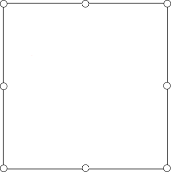
\includegraphics[interpolate=true,width=1.710000in,height=1.720000in]{graph/res/fisica_6sensores-img5.png}}%
\end{pgfscope}%
\begin{pgfscope}%
\definecolor{textcolor}{rgb}{0.000000,0.000000,0.000000}%
\pgfsetstrokecolor{textcolor}%
\pgfsetfillcolor{textcolor}%
\pgftext[x=4.203382in,y=3.956079in,,base]{\color{textcolor}\rmfamily\fontsize{12.000000}{14.400000}\selectfont Error en posición [cm]}%
\end{pgfscope}%
\begin{pgfscope}%
\pgfpathrectangle{\pgfqpoint{5.775845in}{1.127500in}}{\pgfqpoint{0.134750in}{2.695000in}}%
\pgfusepath{clip}%
\pgfsetbuttcap%
\pgfsetmiterjoin%
\definecolor{currentfill}{rgb}{1.000000,1.000000,1.000000}%
\pgfsetfillcolor{currentfill}%
\pgfsetlinewidth{0.010037pt}%
\definecolor{currentstroke}{rgb}{1.000000,1.000000,1.000000}%
\pgfsetstrokecolor{currentstroke}%
\pgfsetdash{}{0pt}%
\pgfpathmoveto{\pgfqpoint{5.775845in}{1.127500in}}%
\pgfpathlineto{\pgfqpoint{5.775845in}{1.138027in}}%
\pgfpathlineto{\pgfqpoint{5.775845in}{3.811973in}}%
\pgfpathlineto{\pgfqpoint{5.775845in}{3.822500in}}%
\pgfpathlineto{\pgfqpoint{5.910595in}{3.822500in}}%
\pgfpathlineto{\pgfqpoint{5.910595in}{3.811973in}}%
\pgfpathlineto{\pgfqpoint{5.910595in}{1.138027in}}%
\pgfpathlineto{\pgfqpoint{5.910595in}{1.127500in}}%
\pgfpathclose%
\pgfusepath{stroke,fill}%
\end{pgfscope}%
\begin{pgfscope}%
\pgfsys@transformshift{5.780000in}{1.130000in}%
\pgftext[left,bottom]{
\includegraphics[interpolate=true,width=0.130000in,height=2.690000in]{graph/res/fisica_6sensores-img6.png}}%
\end{pgfscope}%
\begin{pgfscope}%
\pgfsetbuttcap%
\pgfsetroundjoin%
\definecolor{currentfill}{rgb}{0.000000,0.000000,0.000000}%
\pgfsetfillcolor{currentfill}%
\pgfsetlinewidth{0.803000pt}%
\definecolor{currentstroke}{rgb}{0.000000,0.000000,0.000000}%
\pgfsetstrokecolor{currentstroke}%
\pgfsetdash{}{0pt}%
\pgfsys@defobject{currentmarker}{\pgfqpoint{0.000000in}{0.000000in}}{\pgfqpoint{0.048611in}{0.000000in}}{%
\pgfpathmoveto{\pgfqpoint{0.000000in}{0.000000in}}%
\pgfpathlineto{\pgfqpoint{0.048611in}{0.000000in}}%
\pgfusepath{stroke,fill}%
}%
\begin{pgfscope}%
\pgfsys@transformshift{5.910595in}{1.127500in}%
\pgfsys@useobject{currentmarker}{}%
\end{pgfscope}%
\end{pgfscope}%
\begin{pgfscope}%
\definecolor{textcolor}{rgb}{0.000000,0.000000,0.000000}%
\pgfsetstrokecolor{textcolor}%
\pgfsetfillcolor{textcolor}%
\pgftext[x=6.007818in, y=1.079672in, left, base]{\color{textcolor}\rmfamily\fontsize{10.000000}{12.000000}\selectfont \(\displaystyle {0}\)}%
\end{pgfscope}%
\begin{pgfscope}%
\pgfsetbuttcap%
\pgfsetroundjoin%
\definecolor{currentfill}{rgb}{0.000000,0.000000,0.000000}%
\pgfsetfillcolor{currentfill}%
\pgfsetlinewidth{0.803000pt}%
\definecolor{currentstroke}{rgb}{0.000000,0.000000,0.000000}%
\pgfsetstrokecolor{currentstroke}%
\pgfsetdash{}{0pt}%
\pgfsys@defobject{currentmarker}{\pgfqpoint{0.000000in}{0.000000in}}{\pgfqpoint{0.048611in}{0.000000in}}{%
\pgfpathmoveto{\pgfqpoint{0.000000in}{0.000000in}}%
\pgfpathlineto{\pgfqpoint{0.048611in}{0.000000in}}%
\pgfusepath{stroke,fill}%
}%
\begin{pgfscope}%
\pgfsys@transformshift{5.910595in}{1.432868in}%
\pgfsys@useobject{currentmarker}{}%
\end{pgfscope}%
\end{pgfscope}%
\begin{pgfscope}%
\definecolor{textcolor}{rgb}{0.000000,0.000000,0.000000}%
\pgfsetstrokecolor{textcolor}%
\pgfsetfillcolor{textcolor}%
\pgftext[x=6.007818in, y=1.385040in, left, base]{\color{textcolor}\rmfamily\fontsize{10.000000}{12.000000}\selectfont \(\displaystyle {5}\)}%
\end{pgfscope}%
\begin{pgfscope}%
\pgfsetbuttcap%
\pgfsetroundjoin%
\definecolor{currentfill}{rgb}{0.000000,0.000000,0.000000}%
\pgfsetfillcolor{currentfill}%
\pgfsetlinewidth{0.803000pt}%
\definecolor{currentstroke}{rgb}{0.000000,0.000000,0.000000}%
\pgfsetstrokecolor{currentstroke}%
\pgfsetdash{}{0pt}%
\pgfsys@defobject{currentmarker}{\pgfqpoint{0.000000in}{0.000000in}}{\pgfqpoint{0.048611in}{0.000000in}}{%
\pgfpathmoveto{\pgfqpoint{0.000000in}{0.000000in}}%
\pgfpathlineto{\pgfqpoint{0.048611in}{0.000000in}}%
\pgfusepath{stroke,fill}%
}%
\begin{pgfscope}%
\pgfsys@transformshift{5.910595in}{1.738236in}%
\pgfsys@useobject{currentmarker}{}%
\end{pgfscope}%
\end{pgfscope}%
\begin{pgfscope}%
\definecolor{textcolor}{rgb}{0.000000,0.000000,0.000000}%
\pgfsetstrokecolor{textcolor}%
\pgfsetfillcolor{textcolor}%
\pgftext[x=6.007818in, y=1.690409in, left, base]{\color{textcolor}\rmfamily\fontsize{10.000000}{12.000000}\selectfont \(\displaystyle {10}\)}%
\end{pgfscope}%
\begin{pgfscope}%
\pgfsetbuttcap%
\pgfsetroundjoin%
\definecolor{currentfill}{rgb}{0.000000,0.000000,0.000000}%
\pgfsetfillcolor{currentfill}%
\pgfsetlinewidth{0.803000pt}%
\definecolor{currentstroke}{rgb}{0.000000,0.000000,0.000000}%
\pgfsetstrokecolor{currentstroke}%
\pgfsetdash{}{0pt}%
\pgfsys@defobject{currentmarker}{\pgfqpoint{0.000000in}{0.000000in}}{\pgfqpoint{0.048611in}{0.000000in}}{%
\pgfpathmoveto{\pgfqpoint{0.000000in}{0.000000in}}%
\pgfpathlineto{\pgfqpoint{0.048611in}{0.000000in}}%
\pgfusepath{stroke,fill}%
}%
\begin{pgfscope}%
\pgfsys@transformshift{5.910595in}{2.043605in}%
\pgfsys@useobject{currentmarker}{}%
\end{pgfscope}%
\end{pgfscope}%
\begin{pgfscope}%
\definecolor{textcolor}{rgb}{0.000000,0.000000,0.000000}%
\pgfsetstrokecolor{textcolor}%
\pgfsetfillcolor{textcolor}%
\pgftext[x=6.007818in, y=1.995777in, left, base]{\color{textcolor}\rmfamily\fontsize{10.000000}{12.000000}\selectfont \(\displaystyle {15}\)}%
\end{pgfscope}%
\begin{pgfscope}%
\pgfsetbuttcap%
\pgfsetroundjoin%
\definecolor{currentfill}{rgb}{0.000000,0.000000,0.000000}%
\pgfsetfillcolor{currentfill}%
\pgfsetlinewidth{0.803000pt}%
\definecolor{currentstroke}{rgb}{0.000000,0.000000,0.000000}%
\pgfsetstrokecolor{currentstroke}%
\pgfsetdash{}{0pt}%
\pgfsys@defobject{currentmarker}{\pgfqpoint{0.000000in}{0.000000in}}{\pgfqpoint{0.048611in}{0.000000in}}{%
\pgfpathmoveto{\pgfqpoint{0.000000in}{0.000000in}}%
\pgfpathlineto{\pgfqpoint{0.048611in}{0.000000in}}%
\pgfusepath{stroke,fill}%
}%
\begin{pgfscope}%
\pgfsys@transformshift{5.910595in}{2.348973in}%
\pgfsys@useobject{currentmarker}{}%
\end{pgfscope}%
\end{pgfscope}%
\begin{pgfscope}%
\definecolor{textcolor}{rgb}{0.000000,0.000000,0.000000}%
\pgfsetstrokecolor{textcolor}%
\pgfsetfillcolor{textcolor}%
\pgftext[x=6.007818in, y=2.301145in, left, base]{\color{textcolor}\rmfamily\fontsize{10.000000}{12.000000}\selectfont \(\displaystyle {20}\)}%
\end{pgfscope}%
\begin{pgfscope}%
\pgfsetbuttcap%
\pgfsetroundjoin%
\definecolor{currentfill}{rgb}{0.000000,0.000000,0.000000}%
\pgfsetfillcolor{currentfill}%
\pgfsetlinewidth{0.803000pt}%
\definecolor{currentstroke}{rgb}{0.000000,0.000000,0.000000}%
\pgfsetstrokecolor{currentstroke}%
\pgfsetdash{}{0pt}%
\pgfsys@defobject{currentmarker}{\pgfqpoint{0.000000in}{0.000000in}}{\pgfqpoint{0.048611in}{0.000000in}}{%
\pgfpathmoveto{\pgfqpoint{0.000000in}{0.000000in}}%
\pgfpathlineto{\pgfqpoint{0.048611in}{0.000000in}}%
\pgfusepath{stroke,fill}%
}%
\begin{pgfscope}%
\pgfsys@transformshift{5.910595in}{2.654341in}%
\pgfsys@useobject{currentmarker}{}%
\end{pgfscope}%
\end{pgfscope}%
\begin{pgfscope}%
\definecolor{textcolor}{rgb}{0.000000,0.000000,0.000000}%
\pgfsetstrokecolor{textcolor}%
\pgfsetfillcolor{textcolor}%
\pgftext[x=6.007818in, y=2.606513in, left, base]{\color{textcolor}\rmfamily\fontsize{10.000000}{12.000000}\selectfont \(\displaystyle {25}\)}%
\end{pgfscope}%
\begin{pgfscope}%
\pgfsetbuttcap%
\pgfsetroundjoin%
\definecolor{currentfill}{rgb}{0.000000,0.000000,0.000000}%
\pgfsetfillcolor{currentfill}%
\pgfsetlinewidth{0.803000pt}%
\definecolor{currentstroke}{rgb}{0.000000,0.000000,0.000000}%
\pgfsetstrokecolor{currentstroke}%
\pgfsetdash{}{0pt}%
\pgfsys@defobject{currentmarker}{\pgfqpoint{0.000000in}{0.000000in}}{\pgfqpoint{0.048611in}{0.000000in}}{%
\pgfpathmoveto{\pgfqpoint{0.000000in}{0.000000in}}%
\pgfpathlineto{\pgfqpoint{0.048611in}{0.000000in}}%
\pgfusepath{stroke,fill}%
}%
\begin{pgfscope}%
\pgfsys@transformshift{5.910595in}{2.959709in}%
\pgfsys@useobject{currentmarker}{}%
\end{pgfscope}%
\end{pgfscope}%
\begin{pgfscope}%
\definecolor{textcolor}{rgb}{0.000000,0.000000,0.000000}%
\pgfsetstrokecolor{textcolor}%
\pgfsetfillcolor{textcolor}%
\pgftext[x=6.007818in, y=2.911881in, left, base]{\color{textcolor}\rmfamily\fontsize{10.000000}{12.000000}\selectfont \(\displaystyle {30}\)}%
\end{pgfscope}%
\begin{pgfscope}%
\pgfsetbuttcap%
\pgfsetroundjoin%
\definecolor{currentfill}{rgb}{0.000000,0.000000,0.000000}%
\pgfsetfillcolor{currentfill}%
\pgfsetlinewidth{0.803000pt}%
\definecolor{currentstroke}{rgb}{0.000000,0.000000,0.000000}%
\pgfsetstrokecolor{currentstroke}%
\pgfsetdash{}{0pt}%
\pgfsys@defobject{currentmarker}{\pgfqpoint{0.000000in}{0.000000in}}{\pgfqpoint{0.048611in}{0.000000in}}{%
\pgfpathmoveto{\pgfqpoint{0.000000in}{0.000000in}}%
\pgfpathlineto{\pgfqpoint{0.048611in}{0.000000in}}%
\pgfusepath{stroke,fill}%
}%
\begin{pgfscope}%
\pgfsys@transformshift{5.910595in}{3.265077in}%
\pgfsys@useobject{currentmarker}{}%
\end{pgfscope}%
\end{pgfscope}%
\begin{pgfscope}%
\definecolor{textcolor}{rgb}{0.000000,0.000000,0.000000}%
\pgfsetstrokecolor{textcolor}%
\pgfsetfillcolor{textcolor}%
\pgftext[x=6.007818in, y=3.217249in, left, base]{\color{textcolor}\rmfamily\fontsize{10.000000}{12.000000}\selectfont \(\displaystyle {35}\)}%
\end{pgfscope}%
\begin{pgfscope}%
\pgfsetbuttcap%
\pgfsetroundjoin%
\definecolor{currentfill}{rgb}{0.000000,0.000000,0.000000}%
\pgfsetfillcolor{currentfill}%
\pgfsetlinewidth{0.803000pt}%
\definecolor{currentstroke}{rgb}{0.000000,0.000000,0.000000}%
\pgfsetstrokecolor{currentstroke}%
\pgfsetdash{}{0pt}%
\pgfsys@defobject{currentmarker}{\pgfqpoint{0.000000in}{0.000000in}}{\pgfqpoint{0.048611in}{0.000000in}}{%
\pgfpathmoveto{\pgfqpoint{0.000000in}{0.000000in}}%
\pgfpathlineto{\pgfqpoint{0.048611in}{0.000000in}}%
\pgfusepath{stroke,fill}%
}%
\begin{pgfscope}%
\pgfsys@transformshift{5.910595in}{3.570445in}%
\pgfsys@useobject{currentmarker}{}%
\end{pgfscope}%
\end{pgfscope}%
\begin{pgfscope}%
\definecolor{textcolor}{rgb}{0.000000,0.000000,0.000000}%
\pgfsetstrokecolor{textcolor}%
\pgfsetfillcolor{textcolor}%
\pgftext[x=6.007818in, y=3.522618in, left, base]{\color{textcolor}\rmfamily\fontsize{10.000000}{12.000000}\selectfont \(\displaystyle {40}\)}%
\end{pgfscope}%
\begin{pgfscope}%
\definecolor{textcolor}{rgb}{0.000000,0.000000,0.000000}%
\pgfsetstrokecolor{textcolor}%
\pgfsetfillcolor{textcolor}%
\pgftext[x=6.355040in,y=2.475000in,,top,rotate=270.000000]{\color{textcolor}\rmfamily\fontsize{10.000000}{12.000000}\selectfont Diferencia de posición [cm]}%
\end{pgfscope}%
\begin{pgfscope}%
\pgfsetbuttcap%
\pgfsetmiterjoin%
\pgfsetlinewidth{0.803000pt}%
\definecolor{currentstroke}{rgb}{0.000000,0.000000,0.000000}%
\pgfsetstrokecolor{currentstroke}%
\pgfsetdash{}{0pt}%
\pgfpathmoveto{\pgfqpoint{5.775845in}{1.127500in}}%
\pgfpathlineto{\pgfqpoint{5.775845in}{1.138027in}}%
\pgfpathlineto{\pgfqpoint{5.775845in}{3.811973in}}%
\pgfpathlineto{\pgfqpoint{5.775845in}{3.822500in}}%
\pgfpathlineto{\pgfqpoint{5.910595in}{3.822500in}}%
\pgfpathlineto{\pgfqpoint{5.910595in}{3.811973in}}%
\pgfpathlineto{\pgfqpoint{5.910595in}{1.138027in}}%
\pgfpathlineto{\pgfqpoint{5.910595in}{1.127500in}}%
\pgfpathclose%
\pgfusepath{stroke}%
\end{pgfscope}%
\begin{pgfscope}%
\pgfpathrectangle{\pgfqpoint{0.263486in}{1.323551in}}{\pgfqpoint{0.122303in}{2.446055in}}%
\pgfusepath{clip}%
\pgfsetbuttcap%
\pgfsetmiterjoin%
\definecolor{currentfill}{rgb}{1.000000,1.000000,1.000000}%
\pgfsetfillcolor{currentfill}%
\pgfsetlinewidth{0.010037pt}%
\definecolor{currentstroke}{rgb}{1.000000,1.000000,1.000000}%
\pgfsetstrokecolor{currentstroke}%
\pgfsetdash{}{0pt}%
\pgfpathmoveto{\pgfqpoint{0.263486in}{1.323551in}}%
\pgfpathlineto{\pgfqpoint{0.263486in}{1.333106in}}%
\pgfpathlineto{\pgfqpoint{0.263486in}{3.760051in}}%
\pgfpathlineto{\pgfqpoint{0.263486in}{3.769605in}}%
\pgfpathlineto{\pgfqpoint{0.385789in}{3.769605in}}%
\pgfpathlineto{\pgfqpoint{0.385789in}{3.760051in}}%
\pgfpathlineto{\pgfqpoint{0.385789in}{1.333106in}}%
\pgfpathlineto{\pgfqpoint{0.385789in}{1.323551in}}%
\pgfpathclose%
\pgfusepath{stroke,fill}%
\end{pgfscope}%
\begin{pgfscope}%
\pgfsys@transformshift{0.260000in}{1.320000in}%
\pgftext[left,bottom]{
\includegraphics[interpolate=true,width=0.130000in,height=2.450000in]{graph/res/fisica_6sensores-img7.png}}%
\end{pgfscope}%
\begin{pgfscope}%
\pgfsetbuttcap%
\pgfsetroundjoin%
\definecolor{currentfill}{rgb}{0.000000,0.000000,0.000000}%
\pgfsetfillcolor{currentfill}%
\pgfsetlinewidth{0.803000pt}%
\definecolor{currentstroke}{rgb}{0.000000,0.000000,0.000000}%
\pgfsetstrokecolor{currentstroke}%
\pgfsetdash{}{0pt}%
\pgfsys@defobject{currentmarker}{\pgfqpoint{0.000000in}{0.000000in}}{\pgfqpoint{0.048611in}{0.000000in}}{%
\pgfpathmoveto{\pgfqpoint{0.000000in}{0.000000in}}%
\pgfpathlineto{\pgfqpoint{0.048611in}{0.000000in}}%
\pgfusepath{stroke,fill}%
}%
\begin{pgfscope}%
\pgfsys@transformshift{0.385789in}{1.346601in}%
\pgfsys@useobject{currentmarker}{}%
\end{pgfscope}%
\end{pgfscope}%
\begin{pgfscope}%
\definecolor{textcolor}{rgb}{0.000000,0.000000,0.000000}%
\pgfsetstrokecolor{textcolor}%
\pgfsetfillcolor{textcolor}%
\pgftext[x=0.483011in, y=1.298773in, left, base]{\color{textcolor}\rmfamily\fontsize{10.000000}{12.000000}\selectfont \(\displaystyle {−40}\)}%
\end{pgfscope}%
\begin{pgfscope}%
\pgfsetbuttcap%
\pgfsetroundjoin%
\definecolor{currentfill}{rgb}{0.000000,0.000000,0.000000}%
\pgfsetfillcolor{currentfill}%
\pgfsetlinewidth{0.803000pt}%
\definecolor{currentstroke}{rgb}{0.000000,0.000000,0.000000}%
\pgfsetstrokecolor{currentstroke}%
\pgfsetdash{}{0pt}%
\pgfsys@defobject{currentmarker}{\pgfqpoint{0.000000in}{0.000000in}}{\pgfqpoint{0.048611in}{0.000000in}}{%
\pgfpathmoveto{\pgfqpoint{0.000000in}{0.000000in}}%
\pgfpathlineto{\pgfqpoint{0.048611in}{0.000000in}}%
\pgfusepath{stroke,fill}%
}%
\begin{pgfscope}%
\pgfsys@transformshift{0.385789in}{1.682512in}%
\pgfsys@useobject{currentmarker}{}%
\end{pgfscope}%
\end{pgfscope}%
\begin{pgfscope}%
\definecolor{textcolor}{rgb}{0.000000,0.000000,0.000000}%
\pgfsetstrokecolor{textcolor}%
\pgfsetfillcolor{textcolor}%
\pgftext[x=0.483011in, y=1.634684in, left, base]{\color{textcolor}\rmfamily\fontsize{10.000000}{12.000000}\selectfont \(\displaystyle {−30}\)}%
\end{pgfscope}%
\begin{pgfscope}%
\pgfsetbuttcap%
\pgfsetroundjoin%
\definecolor{currentfill}{rgb}{0.000000,0.000000,0.000000}%
\pgfsetfillcolor{currentfill}%
\pgfsetlinewidth{0.803000pt}%
\definecolor{currentstroke}{rgb}{0.000000,0.000000,0.000000}%
\pgfsetstrokecolor{currentstroke}%
\pgfsetdash{}{0pt}%
\pgfsys@defobject{currentmarker}{\pgfqpoint{0.000000in}{0.000000in}}{\pgfqpoint{0.048611in}{0.000000in}}{%
\pgfpathmoveto{\pgfqpoint{0.000000in}{0.000000in}}%
\pgfpathlineto{\pgfqpoint{0.048611in}{0.000000in}}%
\pgfusepath{stroke,fill}%
}%
\begin{pgfscope}%
\pgfsys@transformshift{0.385789in}{2.018423in}%
\pgfsys@useobject{currentmarker}{}%
\end{pgfscope}%
\end{pgfscope}%
\begin{pgfscope}%
\definecolor{textcolor}{rgb}{0.000000,0.000000,0.000000}%
\pgfsetstrokecolor{textcolor}%
\pgfsetfillcolor{textcolor}%
\pgftext[x=0.483011in, y=1.970595in, left, base]{\color{textcolor}\rmfamily\fontsize{10.000000}{12.000000}\selectfont \(\displaystyle {−20}\)}%
\end{pgfscope}%
\begin{pgfscope}%
\pgfsetbuttcap%
\pgfsetroundjoin%
\definecolor{currentfill}{rgb}{0.000000,0.000000,0.000000}%
\pgfsetfillcolor{currentfill}%
\pgfsetlinewidth{0.803000pt}%
\definecolor{currentstroke}{rgb}{0.000000,0.000000,0.000000}%
\pgfsetstrokecolor{currentstroke}%
\pgfsetdash{}{0pt}%
\pgfsys@defobject{currentmarker}{\pgfqpoint{0.000000in}{0.000000in}}{\pgfqpoint{0.048611in}{0.000000in}}{%
\pgfpathmoveto{\pgfqpoint{0.000000in}{0.000000in}}%
\pgfpathlineto{\pgfqpoint{0.048611in}{0.000000in}}%
\pgfusepath{stroke,fill}%
}%
\begin{pgfscope}%
\pgfsys@transformshift{0.385789in}{2.354334in}%
\pgfsys@useobject{currentmarker}{}%
\end{pgfscope}%
\end{pgfscope}%
\begin{pgfscope}%
\definecolor{textcolor}{rgb}{0.000000,0.000000,0.000000}%
\pgfsetstrokecolor{textcolor}%
\pgfsetfillcolor{textcolor}%
\pgftext[x=0.483011in, y=2.306507in, left, base]{\color{textcolor}\rmfamily\fontsize{10.000000}{12.000000}\selectfont \(\displaystyle {−10}\)}%
\end{pgfscope}%
\begin{pgfscope}%
\pgfsetbuttcap%
\pgfsetroundjoin%
\definecolor{currentfill}{rgb}{0.000000,0.000000,0.000000}%
\pgfsetfillcolor{currentfill}%
\pgfsetlinewidth{0.803000pt}%
\definecolor{currentstroke}{rgb}{0.000000,0.000000,0.000000}%
\pgfsetstrokecolor{currentstroke}%
\pgfsetdash{}{0pt}%
\pgfsys@defobject{currentmarker}{\pgfqpoint{0.000000in}{0.000000in}}{\pgfqpoint{0.048611in}{0.000000in}}{%
\pgfpathmoveto{\pgfqpoint{0.000000in}{0.000000in}}%
\pgfpathlineto{\pgfqpoint{0.048611in}{0.000000in}}%
\pgfusepath{stroke,fill}%
}%
\begin{pgfscope}%
\pgfsys@transformshift{0.385789in}{2.690246in}%
\pgfsys@useobject{currentmarker}{}%
\end{pgfscope}%
\end{pgfscope}%
\begin{pgfscope}%
\definecolor{textcolor}{rgb}{0.000000,0.000000,0.000000}%
\pgfsetstrokecolor{textcolor}%
\pgfsetfillcolor{textcolor}%
\pgftext[x=0.483011in, y=2.642418in, left, base]{\color{textcolor}\rmfamily\fontsize{10.000000}{12.000000}\selectfont \(\displaystyle {0}\)}%
\end{pgfscope}%
\begin{pgfscope}%
\pgfsetbuttcap%
\pgfsetroundjoin%
\definecolor{currentfill}{rgb}{0.000000,0.000000,0.000000}%
\pgfsetfillcolor{currentfill}%
\pgfsetlinewidth{0.803000pt}%
\definecolor{currentstroke}{rgb}{0.000000,0.000000,0.000000}%
\pgfsetstrokecolor{currentstroke}%
\pgfsetdash{}{0pt}%
\pgfsys@defobject{currentmarker}{\pgfqpoint{0.000000in}{0.000000in}}{\pgfqpoint{0.048611in}{0.000000in}}{%
\pgfpathmoveto{\pgfqpoint{0.000000in}{0.000000in}}%
\pgfpathlineto{\pgfqpoint{0.048611in}{0.000000in}}%
\pgfusepath{stroke,fill}%
}%
\begin{pgfscope}%
\pgfsys@transformshift{0.385789in}{3.026157in}%
\pgfsys@useobject{currentmarker}{}%
\end{pgfscope}%
\end{pgfscope}%
\begin{pgfscope}%
\definecolor{textcolor}{rgb}{0.000000,0.000000,0.000000}%
\pgfsetstrokecolor{textcolor}%
\pgfsetfillcolor{textcolor}%
\pgftext[x=0.483011in, y=2.978329in, left, base]{\color{textcolor}\rmfamily\fontsize{10.000000}{12.000000}\selectfont \(\displaystyle {10}\)}%
\end{pgfscope}%
\begin{pgfscope}%
\pgfsetbuttcap%
\pgfsetroundjoin%
\definecolor{currentfill}{rgb}{0.000000,0.000000,0.000000}%
\pgfsetfillcolor{currentfill}%
\pgfsetlinewidth{0.803000pt}%
\definecolor{currentstroke}{rgb}{0.000000,0.000000,0.000000}%
\pgfsetstrokecolor{currentstroke}%
\pgfsetdash{}{0pt}%
\pgfsys@defobject{currentmarker}{\pgfqpoint{0.000000in}{0.000000in}}{\pgfqpoint{0.048611in}{0.000000in}}{%
\pgfpathmoveto{\pgfqpoint{0.000000in}{0.000000in}}%
\pgfpathlineto{\pgfqpoint{0.048611in}{0.000000in}}%
\pgfusepath{stroke,fill}%
}%
\begin{pgfscope}%
\pgfsys@transformshift{0.385789in}{3.362068in}%
\pgfsys@useobject{currentmarker}{}%
\end{pgfscope}%
\end{pgfscope}%
\begin{pgfscope}%
\definecolor{textcolor}{rgb}{0.000000,0.000000,0.000000}%
\pgfsetstrokecolor{textcolor}%
\pgfsetfillcolor{textcolor}%
\pgftext[x=0.483011in, y=3.314240in, left, base]{\color{textcolor}\rmfamily\fontsize{10.000000}{12.000000}\selectfont \(\displaystyle {20}\)}%
\end{pgfscope}%
\begin{pgfscope}%
\pgfsetbuttcap%
\pgfsetroundjoin%
\definecolor{currentfill}{rgb}{0.000000,0.000000,0.000000}%
\pgfsetfillcolor{currentfill}%
\pgfsetlinewidth{0.803000pt}%
\definecolor{currentstroke}{rgb}{0.000000,0.000000,0.000000}%
\pgfsetstrokecolor{currentstroke}%
\pgfsetdash{}{0pt}%
\pgfsys@defobject{currentmarker}{\pgfqpoint{0.000000in}{0.000000in}}{\pgfqpoint{0.048611in}{0.000000in}}{%
\pgfpathmoveto{\pgfqpoint{0.000000in}{0.000000in}}%
\pgfpathlineto{\pgfqpoint{0.048611in}{0.000000in}}%
\pgfusepath{stroke,fill}%
}%
\begin{pgfscope}%
\pgfsys@transformshift{0.385789in}{3.697979in}%
\pgfsys@useobject{currentmarker}{}%
\end{pgfscope}%
\end{pgfscope}%
\begin{pgfscope}%
\definecolor{textcolor}{rgb}{0.000000,0.000000,0.000000}%
\pgfsetstrokecolor{textcolor}%
\pgfsetfillcolor{textcolor}%
\pgftext[x=0.483011in, y=3.650152in, left, base]{\color{textcolor}\rmfamily\fontsize{10.000000}{12.000000}\selectfont \(\displaystyle {30}\)}%
\end{pgfscope}%
\begin{pgfscope}%
\definecolor{textcolor}{rgb}{0.000000,0.000000,0.000000}%
\pgfsetstrokecolor{textcolor}%
\pgfsetfillcolor{textcolor}%
\pgftext[x=0.035481in,y=2.546578in,,top,rotate=90.000000]{\color{textcolor}\rmfamily\fontsize{10.000000}{12.000000}\selectfont Diferencia en la medida de cada eje [cm]}%
\end{pgfscope}%
\begin{pgfscope}%
\pgfsetbuttcap%
\pgfsetmiterjoin%
\pgfsetlinewidth{0.803000pt}%
\definecolor{currentstroke}{rgb}{0.000000,0.000000,0.000000}%
\pgfsetstrokecolor{currentstroke}%
\pgfsetdash{}{0pt}%
\pgfpathmoveto{\pgfqpoint{0.263486in}{1.323551in}}%
\pgfpathlineto{\pgfqpoint{0.263486in}{1.333106in}}%
\pgfpathlineto{\pgfqpoint{0.263486in}{3.760051in}}%
\pgfpathlineto{\pgfqpoint{0.263486in}{3.769605in}}%
\pgfpathlineto{\pgfqpoint{0.385789in}{3.769605in}}%
\pgfpathlineto{\pgfqpoint{0.385789in}{3.760051in}}%
\pgfpathlineto{\pgfqpoint{0.385789in}{1.333106in}}%
\pgfpathlineto{\pgfqpoint{0.385789in}{1.323551in}}%
\pgfpathclose%
\pgfusepath{stroke}%
\end{pgfscope}%
\end{pgfpicture}%
\makeatother%
\endgroup%

  \caption{Resultados de las medidas en el edificio de Física con 6 balizas. Entre paréntesis se indica la desviación estándar de los errores obtenidos en cada punto.}
  \label{fig:res_fisica_6}
\end{figure}

Aunque los resultados en este caso son mejores, se sigue encontrando el máximo en el punto 10.
Es más, los valores desde el punto 9 al 13 no tienen una mejora significativa con 6 balizas debido a la posición de la baliza adicional en esa pared.

Este efecto ya fue discutido en el análisis de las medidas del laboratorio.
Una de las conclusiones en aquel caso era que una distribución uniforme de las balizas proporcionaba mejores resultados, y no simplemente un número mayor sin considerar su posición.

Debido a la distribución de la planta, las dos balizas más cercanas a los puntos mencionados se colocaron a poco más de dos metros entre ellas.
Esta escasa separación hace que las medidas en las que se ven utilizadas no presenten una gran mejora respecto a los casos en los que solo una de ellas participaba en los cálculos.

\begin{table}[H]
  \hspace*{-0.5cm}
  \centering
  \begin{tabular}{c|c|c|c|c|c|}
    \cline{2-6}
                                              & \begin{tabular}[c]{@{}c@{}}Error en \\ eje $x$ (cm) \end{tabular} & \begin{tabular}[c]{@{}c@{}} Error en \\ eje $y$ (cm) \end{tabular} & \begin{tabular}[c]{@{}c@{}} Error en eje $x$ \\ (absoluto) (cm) \end{tabular} & \begin{tabular}[c]{@{}c@{}} Error en eje $y$ \\ (absoluto) (cm) \end{tabular} & \begin{tabular}[c]{@{}c@{}} Error en \\ posición(cm) \end{tabular}\\ \hline
    \multicolumn{1}{|c|}{Media}               &  -4.7   &   -11.9 &      16.0          &         12.1       &  23.7    \\ \hline
    \multicolumn{1}{|c|}{Mediana}             &  -3.8   &   -10.4 &      17.7          &         10.3       &  22.7    \\ \hline
    \multicolumn{1}{|c|}{Desv. estándar} &   18.7  &   10.5  &      10.8          &         10.1       &  10.9    \\ \hline
    \multicolumn{1}{|c|}{Máximo}              &   32.1  &   1.1   &      40.8          &         30.8       &  44.1    \\ \hline
    \multicolumn{1}{|c|}{Mínimo}              &  -40.7  &   -30.9 &      3.3           &         0.4        &  7.8     \\ \hline
\end{tabular}
\caption{Resumen de los errores en el edificio de Física con 6 balizas.}
\label{tab:media_fisica_6}
\end{table}

A pesar de las escasas mejoras en los puntos mencionados anteriormente, los valores medios recogidos en la Tabla \ref{tab:media_fisica_6} sí que presentan mejoras significativas en esta configuración con más balizas.

\subsubsection{8 balizas}

Por último, se añadieron otros dos sensores para tener 8 balizas tal y como se muestra en la Figura~\ref{fig:sensores_fisica_8}, tras lo que se obtuvieron los resultados representados en la Figura~\ref{fig:res_fisica_8} y recogidos en la Tabla~\ref{tab:media_fisica_8_total}.
\begin{figure}[H]
    \centering
    %% Creator: Matplotlib, PGF backend
%%
%% To include the figure in your LaTeX document, write
%%   \input{<filename>.pgf}
%%
%% Make sure the required packages are loaded in your preamble
%%   \usepackage{pgf}
%%
%% and, on pdftex
%%   \usepackage[utf8]{inputenc}\DeclareUnicodeCharacter{2212}{-}
%%
%% or, on luatex and xetex
%%   \usepackage{unicode-math}
%%
%% Figures using additional raster images can only be included by \input if
%% they are in the same directory as the main LaTeX file. For loading figures
%% from other directories you can use the `import` package
%%   \usepackage{import}
%%
%% and then include the figures with
%%   \import{<path to file>}{<filename>.pgf}
%%
%% Matplotlib used the following preamble
%%   \usepackage[utf8x]{inputenc}
%%   \usepackage[T1]{fontenc}
%%
\begingroup%
\makeatletter%
\begin{pgfpicture}%
\pgfpathrectangle{\pgfpointorigin}{\pgfqpoint{7.000000in}{5.000000in}}%
\pgfusepath{use as bounding box, clip}%
\begin{pgfscope}%
\pgfsetbuttcap%
\pgfsetmiterjoin%
\definecolor{currentfill}{rgb}{1.000000,1.000000,1.000000}%
\pgfsetfillcolor{currentfill}%
\pgfsetlinewidth{0.000000pt}%
\definecolor{currentstroke}{rgb}{1.000000,1.000000,1.000000}%
\pgfsetstrokecolor{currentstroke}%
\pgfsetdash{}{0pt}%
\pgfpathmoveto{\pgfqpoint{0.000000in}{0.000000in}}%
\pgfpathlineto{\pgfqpoint{7.000000in}{0.000000in}}%
\pgfpathlineto{\pgfqpoint{7.000000in}{5.000000in}}%
\pgfpathlineto{\pgfqpoint{0.000000in}{5.000000in}}%
\pgfpathclose%
\pgfusepath{fill}%
\end{pgfscope}%
\begin{pgfscope}%
\pgfsetbuttcap%
\pgfsetmiterjoin%
\definecolor{currentfill}{rgb}{1.000000,1.000000,1.000000}%
\pgfsetfillcolor{currentfill}%
\pgfsetlinewidth{0.000000pt}%
\definecolor{currentstroke}{rgb}{0.000000,0.000000,0.000000}%
\pgfsetstrokecolor{currentstroke}%
\pgfsetstrokeopacity{0.000000}%
\pgfsetdash{}{0pt}%
\pgfpathmoveto{\pgfqpoint{0.875000in}{2.913486in}}%
\pgfpathlineto{\pgfqpoint{2.098027in}{2.913486in}}%
\pgfpathlineto{\pgfqpoint{2.098027in}{4.136514in}}%
\pgfpathlineto{\pgfqpoint{0.875000in}{4.136514in}}%
\pgfpathclose%
\pgfusepath{fill}%
\end{pgfscope}%
\begin{pgfscope}%
\pgfpathrectangle{\pgfqpoint{0.875000in}{2.913486in}}{\pgfqpoint{1.223027in}{1.223027in}}%
\pgfusepath{clip}%
\pgfsys@transformshift{0.875000in}{2.913486in}%
\pgftext[left,bottom]{
\includegraphics[interpolate=true,width=1.230000in,height=1.230000in]{graph/res/fisica_8sensores-img0.png}}%
\end{pgfscope}%
\begin{pgfscope}%
\pgfsetrectcap%
\pgfsetmiterjoin%
\pgfsetlinewidth{0.803000pt}%
\definecolor{currentstroke}{rgb}{0.000000,0.000000,0.000000}%
\pgfsetstrokecolor{currentstroke}%
\pgfsetdash{}{0pt}%
\pgfpathmoveto{\pgfqpoint{0.875000in}{2.913486in}}%
\pgfpathlineto{\pgfqpoint{0.875000in}{4.136514in}}%
\pgfusepath{stroke}%
\end{pgfscope}%
\begin{pgfscope}%
\pgfsetrectcap%
\pgfsetmiterjoin%
\pgfsetlinewidth{0.803000pt}%
\definecolor{currentstroke}{rgb}{0.000000,0.000000,0.000000}%
\pgfsetstrokecolor{currentstroke}%
\pgfsetdash{}{0pt}%
\pgfpathmoveto{\pgfqpoint{2.098027in}{2.913486in}}%
\pgfpathlineto{\pgfqpoint{2.098027in}{4.136514in}}%
\pgfusepath{stroke}%
\end{pgfscope}%
\begin{pgfscope}%
\pgfsetrectcap%
\pgfsetmiterjoin%
\pgfsetlinewidth{0.803000pt}%
\definecolor{currentstroke}{rgb}{0.000000,0.000000,0.000000}%
\pgfsetstrokecolor{currentstroke}%
\pgfsetdash{}{0pt}%
\pgfpathmoveto{\pgfqpoint{0.875000in}{2.913486in}}%
\pgfpathlineto{\pgfqpoint{2.098027in}{2.913486in}}%
\pgfusepath{stroke}%
\end{pgfscope}%
\begin{pgfscope}%
\pgfsetrectcap%
\pgfsetmiterjoin%
\pgfsetlinewidth{0.803000pt}%
\definecolor{currentstroke}{rgb}{0.000000,0.000000,0.000000}%
\pgfsetstrokecolor{currentstroke}%
\pgfsetdash{}{0pt}%
\pgfpathmoveto{\pgfqpoint{0.875000in}{4.136514in}}%
\pgfpathlineto{\pgfqpoint{2.098027in}{4.136514in}}%
\pgfusepath{stroke}%
\end{pgfscope}%
\begin{pgfscope}%
\pgfsys@transformshift{1.060264in}{3.095000in}%
\pgftext[left,bottom]{
\includegraphics[interpolate=true,width=0.860000in,height=0.860000in]{graph/res/fisica_8sensores-img1.png}}%
\end{pgfscope}%
\begin{pgfscope}%
\definecolor{textcolor}{rgb}{0.000000,0.000000,0.000000}%
\pgfsetstrokecolor{textcolor}%
\pgfsetfillcolor{textcolor}%
\pgftext[x=1.486514in,y=4.219847in,,base]{\color{textcolor}\rmfamily\fontsize{12.000000}{14.400000}\selectfont Error en eje $x$}%
\end{pgfscope}%
\begin{pgfscope}%
\pgfsetbuttcap%
\pgfsetmiterjoin%
\definecolor{currentfill}{rgb}{1.000000,1.000000,1.000000}%
\pgfsetfillcolor{currentfill}%
\pgfsetlinewidth{0.000000pt}%
\definecolor{currentstroke}{rgb}{0.000000,0.000000,0.000000}%
\pgfsetstrokecolor{currentstroke}%
\pgfsetstrokeopacity{0.000000}%
\pgfsetdash{}{0pt}%
\pgfpathmoveto{\pgfqpoint{0.875000in}{0.813486in}}%
\pgfpathlineto{\pgfqpoint{2.098027in}{0.813486in}}%
\pgfpathlineto{\pgfqpoint{2.098027in}{2.036514in}}%
\pgfpathlineto{\pgfqpoint{0.875000in}{2.036514in}}%
\pgfpathclose%
\pgfusepath{fill}%
\end{pgfscope}%
\begin{pgfscope}%
\pgfpathrectangle{\pgfqpoint{0.875000in}{0.813486in}}{\pgfqpoint{1.223027in}{1.223027in}}%
\pgfusepath{clip}%
\pgfsys@transformshift{0.875000in}{0.813486in}%
\pgftext[left,bottom]{
\includegraphics[interpolate=true,width=1.230000in,height=1.230000in]{graph/res/fisica_8sensores-img2.png}}%
\end{pgfscope}%
\begin{pgfscope}%
\pgfsetrectcap%
\pgfsetmiterjoin%
\pgfsetlinewidth{0.803000pt}%
\definecolor{currentstroke}{rgb}{0.000000,0.000000,0.000000}%
\pgfsetstrokecolor{currentstroke}%
\pgfsetdash{}{0pt}%
\pgfpathmoveto{\pgfqpoint{0.875000in}{0.813486in}}%
\pgfpathlineto{\pgfqpoint{0.875000in}{2.036514in}}%
\pgfusepath{stroke}%
\end{pgfscope}%
\begin{pgfscope}%
\pgfsetrectcap%
\pgfsetmiterjoin%
\pgfsetlinewidth{0.803000pt}%
\definecolor{currentstroke}{rgb}{0.000000,0.000000,0.000000}%
\pgfsetstrokecolor{currentstroke}%
\pgfsetdash{}{0pt}%
\pgfpathmoveto{\pgfqpoint{2.098027in}{0.813486in}}%
\pgfpathlineto{\pgfqpoint{2.098027in}{2.036514in}}%
\pgfusepath{stroke}%
\end{pgfscope}%
\begin{pgfscope}%
\pgfsetrectcap%
\pgfsetmiterjoin%
\pgfsetlinewidth{0.803000pt}%
\definecolor{currentstroke}{rgb}{0.000000,0.000000,0.000000}%
\pgfsetstrokecolor{currentstroke}%
\pgfsetdash{}{0pt}%
\pgfpathmoveto{\pgfqpoint{0.875000in}{0.813486in}}%
\pgfpathlineto{\pgfqpoint{2.098027in}{0.813486in}}%
\pgfusepath{stroke}%
\end{pgfscope}%
\begin{pgfscope}%
\pgfsetrectcap%
\pgfsetmiterjoin%
\pgfsetlinewidth{0.803000pt}%
\definecolor{currentstroke}{rgb}{0.000000,0.000000,0.000000}%
\pgfsetstrokecolor{currentstroke}%
\pgfsetdash{}{0pt}%
\pgfpathmoveto{\pgfqpoint{0.875000in}{2.036514in}}%
\pgfpathlineto{\pgfqpoint{2.098027in}{2.036514in}}%
\pgfusepath{stroke}%
\end{pgfscope}%
\begin{pgfscope}%
\pgfsys@transformshift{1.060264in}{0.995000in}%
\pgftext[left,bottom]{
\includegraphics[interpolate=true,width=0.860000in,height=0.860000in]{graph/res/fisica_8sensores-img3.png}}%
\end{pgfscope}%
\begin{pgfscope}%
\definecolor{textcolor}{rgb}{0.000000,0.000000,0.000000}%
\pgfsetstrokecolor{textcolor}%
\pgfsetfillcolor{textcolor}%
\pgftext[x=1.486514in,y=2.119847in,,base]{\color{textcolor}\rmfamily\fontsize{12.000000}{14.400000}\selectfont Error en eje $y$}%
\end{pgfscope}%
\begin{pgfscope}%
\pgfsetbuttcap%
\pgfsetmiterjoin%
\definecolor{currentfill}{rgb}{1.000000,1.000000,1.000000}%
\pgfsetfillcolor{currentfill}%
\pgfsetlinewidth{0.000000pt}%
\definecolor{currentstroke}{rgb}{0.000000,0.000000,0.000000}%
\pgfsetstrokecolor{currentstroke}%
\pgfsetstrokeopacity{0.000000}%
\pgfsetdash{}{0pt}%
\pgfpathmoveto{\pgfqpoint{2.805636in}{1.077254in}}%
\pgfpathlineto{\pgfqpoint{5.601127in}{1.077254in}}%
\pgfpathlineto{\pgfqpoint{5.601127in}{3.872746in}}%
\pgfpathlineto{\pgfqpoint{2.805636in}{3.872746in}}%
\pgfpathclose%
\pgfusepath{fill}%
\end{pgfscope}%
\begin{pgfscope}%
\pgfpathrectangle{\pgfqpoint{2.805636in}{1.077254in}}{\pgfqpoint{2.795491in}{2.795491in}}%
\pgfusepath{clip}%
\pgfsys@transformshift{2.805636in}{1.077254in}%
\pgftext[left,bottom]{
\includegraphics[interpolate=true,width=2.800000in,height=2.800000in]{graph/res/fisica_8sensores-img4.png}}%
\end{pgfscope}%
\begin{pgfscope}%
\pgfsetbuttcap%
\pgfsetroundjoin%
\definecolor{currentfill}{rgb}{0.000000,0.000000,0.000000}%
\pgfsetfillcolor{currentfill}%
\pgfsetlinewidth{0.803000pt}%
\definecolor{currentstroke}{rgb}{0.000000,0.000000,0.000000}%
\pgfsetstrokecolor{currentstroke}%
\pgfsetdash{}{0pt}%
\pgfsys@defobject{currentmarker}{\pgfqpoint{0.000000in}{-0.048611in}}{\pgfqpoint{0.000000in}{0.000000in}}{%
\pgfpathmoveto{\pgfqpoint{0.000000in}{0.000000in}}%
\pgfpathlineto{\pgfqpoint{0.000000in}{-0.048611in}}%
\pgfusepath{stroke,fill}%
}%
\begin{pgfscope}%
\pgfsys@transformshift{3.085185in}{1.077254in}%
\pgfsys@useobject{currentmarker}{}%
\end{pgfscope}%
\end{pgfscope}%
\begin{pgfscope}%
\definecolor{textcolor}{rgb}{0.000000,0.000000,0.000000}%
\pgfsetstrokecolor{textcolor}%
\pgfsetfillcolor{textcolor}%
\pgftext[x=3.085185in,y=0.980032in,,top]{\color{textcolor}\rmfamily\fontsize{10.000000}{12.000000}\selectfont 1.0}%
\end{pgfscope}%
\begin{pgfscope}%
\pgfsetbuttcap%
\pgfsetroundjoin%
\definecolor{currentfill}{rgb}{0.000000,0.000000,0.000000}%
\pgfsetfillcolor{currentfill}%
\pgfsetlinewidth{0.803000pt}%
\definecolor{currentstroke}{rgb}{0.000000,0.000000,0.000000}%
\pgfsetstrokecolor{currentstroke}%
\pgfsetdash{}{0pt}%
\pgfsys@defobject{currentmarker}{\pgfqpoint{0.000000in}{-0.048611in}}{\pgfqpoint{0.000000in}{0.000000in}}{%
\pgfpathmoveto{\pgfqpoint{0.000000in}{0.000000in}}%
\pgfpathlineto{\pgfqpoint{0.000000in}{-0.048611in}}%
\pgfusepath{stroke,fill}%
}%
\begin{pgfscope}%
\pgfsys@transformshift{3.644283in}{1.077254in}%
\pgfsys@useobject{currentmarker}{}%
\end{pgfscope}%
\end{pgfscope}%
\begin{pgfscope}%
\definecolor{textcolor}{rgb}{0.000000,0.000000,0.000000}%
\pgfsetstrokecolor{textcolor}%
\pgfsetfillcolor{textcolor}%
\pgftext[x=3.644283in,y=0.980032in,,top]{\color{textcolor}\rmfamily\fontsize{10.000000}{12.000000}\selectfont 3.25}%
\end{pgfscope}%
\begin{pgfscope}%
\pgfsetbuttcap%
\pgfsetroundjoin%
\definecolor{currentfill}{rgb}{0.000000,0.000000,0.000000}%
\pgfsetfillcolor{currentfill}%
\pgfsetlinewidth{0.803000pt}%
\definecolor{currentstroke}{rgb}{0.000000,0.000000,0.000000}%
\pgfsetstrokecolor{currentstroke}%
\pgfsetdash{}{0pt}%
\pgfsys@defobject{currentmarker}{\pgfqpoint{0.000000in}{-0.048611in}}{\pgfqpoint{0.000000in}{0.000000in}}{%
\pgfpathmoveto{\pgfqpoint{0.000000in}{0.000000in}}%
\pgfpathlineto{\pgfqpoint{0.000000in}{-0.048611in}}%
\pgfusepath{stroke,fill}%
}%
\begin{pgfscope}%
\pgfsys@transformshift{4.203382in}{1.077254in}%
\pgfsys@useobject{currentmarker}{}%
\end{pgfscope}%
\end{pgfscope}%
\begin{pgfscope}%
\definecolor{textcolor}{rgb}{0.000000,0.000000,0.000000}%
\pgfsetstrokecolor{textcolor}%
\pgfsetfillcolor{textcolor}%
\pgftext[x=4.203382in,y=0.980032in,,top]{\color{textcolor}\rmfamily\fontsize{10.000000}{12.000000}\selectfont 5.5}%
\end{pgfscope}%
\begin{pgfscope}%
\pgfsetbuttcap%
\pgfsetroundjoin%
\definecolor{currentfill}{rgb}{0.000000,0.000000,0.000000}%
\pgfsetfillcolor{currentfill}%
\pgfsetlinewidth{0.803000pt}%
\definecolor{currentstroke}{rgb}{0.000000,0.000000,0.000000}%
\pgfsetstrokecolor{currentstroke}%
\pgfsetdash{}{0pt}%
\pgfsys@defobject{currentmarker}{\pgfqpoint{0.000000in}{-0.048611in}}{\pgfqpoint{0.000000in}{0.000000in}}{%
\pgfpathmoveto{\pgfqpoint{0.000000in}{0.000000in}}%
\pgfpathlineto{\pgfqpoint{0.000000in}{-0.048611in}}%
\pgfusepath{stroke,fill}%
}%
\begin{pgfscope}%
\pgfsys@transformshift{4.762480in}{1.077254in}%
\pgfsys@useobject{currentmarker}{}%
\end{pgfscope}%
\end{pgfscope}%
\begin{pgfscope}%
\definecolor{textcolor}{rgb}{0.000000,0.000000,0.000000}%
\pgfsetstrokecolor{textcolor}%
\pgfsetfillcolor{textcolor}%
\pgftext[x=4.762480in,y=0.980032in,,top]{\color{textcolor}\rmfamily\fontsize{10.000000}{12.000000}\selectfont 7.75}%
\end{pgfscope}%
\begin{pgfscope}%
\pgfsetbuttcap%
\pgfsetroundjoin%
\definecolor{currentfill}{rgb}{0.000000,0.000000,0.000000}%
\pgfsetfillcolor{currentfill}%
\pgfsetlinewidth{0.803000pt}%
\definecolor{currentstroke}{rgb}{0.000000,0.000000,0.000000}%
\pgfsetstrokecolor{currentstroke}%
\pgfsetdash{}{0pt}%
\pgfsys@defobject{currentmarker}{\pgfqpoint{0.000000in}{-0.048611in}}{\pgfqpoint{0.000000in}{0.000000in}}{%
\pgfpathmoveto{\pgfqpoint{0.000000in}{0.000000in}}%
\pgfpathlineto{\pgfqpoint{0.000000in}{-0.048611in}}%
\pgfusepath{stroke,fill}%
}%
\begin{pgfscope}%
\pgfsys@transformshift{5.321578in}{1.077254in}%
\pgfsys@useobject{currentmarker}{}%
\end{pgfscope}%
\end{pgfscope}%
\begin{pgfscope}%
\definecolor{textcolor}{rgb}{0.000000,0.000000,0.000000}%
\pgfsetstrokecolor{textcolor}%
\pgfsetfillcolor{textcolor}%
\pgftext[x=5.321578in,y=0.980032in,,top]{\color{textcolor}\rmfamily\fontsize{10.000000}{12.000000}\selectfont 10.0}%
\end{pgfscope}%
\begin{pgfscope}%
\definecolor{textcolor}{rgb}{0.000000,0.000000,0.000000}%
\pgfsetstrokecolor{textcolor}%
\pgfsetfillcolor{textcolor}%
\pgftext[x=4.203382in,y=0.801822in,,top]{\color{textcolor}\rmfamily\fontsize{10.000000}{12.000000}\selectfont x [m]}%
\end{pgfscope}%
\begin{pgfscope}%
\pgfsetbuttcap%
\pgfsetroundjoin%
\definecolor{currentfill}{rgb}{0.000000,0.000000,0.000000}%
\pgfsetfillcolor{currentfill}%
\pgfsetlinewidth{0.803000pt}%
\definecolor{currentstroke}{rgb}{0.000000,0.000000,0.000000}%
\pgfsetstrokecolor{currentstroke}%
\pgfsetdash{}{0pt}%
\pgfsys@defobject{currentmarker}{\pgfqpoint{-0.048611in}{0.000000in}}{\pgfqpoint{-0.000000in}{0.000000in}}{%
\pgfpathmoveto{\pgfqpoint{-0.000000in}{0.000000in}}%
\pgfpathlineto{\pgfqpoint{-0.048611in}{0.000000in}}%
\pgfusepath{stroke,fill}%
}%
\begin{pgfscope}%
\pgfsys@transformshift{2.805636in}{1.356804in}%
\pgfsys@useobject{currentmarker}{}%
\end{pgfscope}%
\end{pgfscope}%
\begin{pgfscope}%
\definecolor{textcolor}{rgb}{0.000000,0.000000,0.000000}%
\pgfsetstrokecolor{textcolor}%
\pgfsetfillcolor{textcolor}%
\pgftext[x=2.530988in, y=1.308976in, left, base]{\color{textcolor}\rmfamily\fontsize{10.000000}{12.000000}\selectfont 1.0}%
\end{pgfscope}%
\begin{pgfscope}%
\pgfsetbuttcap%
\pgfsetroundjoin%
\definecolor{currentfill}{rgb}{0.000000,0.000000,0.000000}%
\pgfsetfillcolor{currentfill}%
\pgfsetlinewidth{0.803000pt}%
\definecolor{currentstroke}{rgb}{0.000000,0.000000,0.000000}%
\pgfsetstrokecolor{currentstroke}%
\pgfsetdash{}{0pt}%
\pgfsys@defobject{currentmarker}{\pgfqpoint{-0.048611in}{0.000000in}}{\pgfqpoint{-0.000000in}{0.000000in}}{%
\pgfpathmoveto{\pgfqpoint{-0.000000in}{0.000000in}}%
\pgfpathlineto{\pgfqpoint{-0.048611in}{0.000000in}}%
\pgfusepath{stroke,fill}%
}%
\begin{pgfscope}%
\pgfsys@transformshift{2.805636in}{1.915902in}%
\pgfsys@useobject{currentmarker}{}%
\end{pgfscope}%
\end{pgfscope}%
\begin{pgfscope}%
\definecolor{textcolor}{rgb}{0.000000,0.000000,0.000000}%
\pgfsetstrokecolor{textcolor}%
\pgfsetfillcolor{textcolor}%
\pgftext[x=2.461561in, y=1.868074in, left, base]{\color{textcolor}\rmfamily\fontsize{10.000000}{12.000000}\selectfont 3.25}%
\end{pgfscope}%
\begin{pgfscope}%
\pgfsetbuttcap%
\pgfsetroundjoin%
\definecolor{currentfill}{rgb}{0.000000,0.000000,0.000000}%
\pgfsetfillcolor{currentfill}%
\pgfsetlinewidth{0.803000pt}%
\definecolor{currentstroke}{rgb}{0.000000,0.000000,0.000000}%
\pgfsetstrokecolor{currentstroke}%
\pgfsetdash{}{0pt}%
\pgfsys@defobject{currentmarker}{\pgfqpoint{-0.048611in}{0.000000in}}{\pgfqpoint{-0.000000in}{0.000000in}}{%
\pgfpathmoveto{\pgfqpoint{-0.000000in}{0.000000in}}%
\pgfpathlineto{\pgfqpoint{-0.048611in}{0.000000in}}%
\pgfusepath{stroke,fill}%
}%
\begin{pgfscope}%
\pgfsys@transformshift{2.805636in}{2.475000in}%
\pgfsys@useobject{currentmarker}{}%
\end{pgfscope}%
\end{pgfscope}%
\begin{pgfscope}%
\definecolor{textcolor}{rgb}{0.000000,0.000000,0.000000}%
\pgfsetstrokecolor{textcolor}%
\pgfsetfillcolor{textcolor}%
\pgftext[x=2.530988in, y=2.427172in, left, base]{\color{textcolor}\rmfamily\fontsize{10.000000}{12.000000}\selectfont 5.5}%
\end{pgfscope}%
\begin{pgfscope}%
\pgfsetbuttcap%
\pgfsetroundjoin%
\definecolor{currentfill}{rgb}{0.000000,0.000000,0.000000}%
\pgfsetfillcolor{currentfill}%
\pgfsetlinewidth{0.803000pt}%
\definecolor{currentstroke}{rgb}{0.000000,0.000000,0.000000}%
\pgfsetstrokecolor{currentstroke}%
\pgfsetdash{}{0pt}%
\pgfsys@defobject{currentmarker}{\pgfqpoint{-0.048611in}{0.000000in}}{\pgfqpoint{-0.000000in}{0.000000in}}{%
\pgfpathmoveto{\pgfqpoint{-0.000000in}{0.000000in}}%
\pgfpathlineto{\pgfqpoint{-0.048611in}{0.000000in}}%
\pgfusepath{stroke,fill}%
}%
\begin{pgfscope}%
\pgfsys@transformshift{2.805636in}{3.034098in}%
\pgfsys@useobject{currentmarker}{}%
\end{pgfscope}%
\end{pgfscope}%
\begin{pgfscope}%
\definecolor{textcolor}{rgb}{0.000000,0.000000,0.000000}%
\pgfsetstrokecolor{textcolor}%
\pgfsetfillcolor{textcolor}%
\pgftext[x=2.461561in, y=2.986270in, left, base]{\color{textcolor}\rmfamily\fontsize{10.000000}{12.000000}\selectfont 7.75}%
\end{pgfscope}%
\begin{pgfscope}%
\pgfsetbuttcap%
\pgfsetroundjoin%
\definecolor{currentfill}{rgb}{0.000000,0.000000,0.000000}%
\pgfsetfillcolor{currentfill}%
\pgfsetlinewidth{0.803000pt}%
\definecolor{currentstroke}{rgb}{0.000000,0.000000,0.000000}%
\pgfsetstrokecolor{currentstroke}%
\pgfsetdash{}{0pt}%
\pgfsys@defobject{currentmarker}{\pgfqpoint{-0.048611in}{0.000000in}}{\pgfqpoint{-0.000000in}{0.000000in}}{%
\pgfpathmoveto{\pgfqpoint{-0.000000in}{0.000000in}}%
\pgfpathlineto{\pgfqpoint{-0.048611in}{0.000000in}}%
\pgfusepath{stroke,fill}%
}%
\begin{pgfscope}%
\pgfsys@transformshift{2.805636in}{3.593196in}%
\pgfsys@useobject{currentmarker}{}%
\end{pgfscope}%
\end{pgfscope}%
\begin{pgfscope}%
\definecolor{textcolor}{rgb}{0.000000,0.000000,0.000000}%
\pgfsetstrokecolor{textcolor}%
\pgfsetfillcolor{textcolor}%
\pgftext[x=2.461561in, y=3.545369in, left, base]{\color{textcolor}\rmfamily\fontsize{10.000000}{12.000000}\selectfont 10.0}%
\end{pgfscope}%
\begin{pgfscope}%
\definecolor{textcolor}{rgb}{0.000000,0.000000,0.000000}%
\pgfsetstrokecolor{textcolor}%
\pgfsetfillcolor{textcolor}%
\pgftext[x=2.406005in,y=2.475000in,,bottom,rotate=90.000000]{\color{textcolor}\rmfamily\fontsize{10.000000}{12.000000}\selectfont y [m]}%
\end{pgfscope}%
\begin{pgfscope}%
\pgfsetrectcap%
\pgfsetmiterjoin%
\pgfsetlinewidth{0.803000pt}%
\definecolor{currentstroke}{rgb}{0.000000,0.000000,0.000000}%
\pgfsetstrokecolor{currentstroke}%
\pgfsetdash{}{0pt}%
\pgfpathmoveto{\pgfqpoint{2.805636in}{1.077254in}}%
\pgfpathlineto{\pgfqpoint{2.805636in}{3.872746in}}%
\pgfusepath{stroke}%
\end{pgfscope}%
\begin{pgfscope}%
\pgfsetrectcap%
\pgfsetmiterjoin%
\pgfsetlinewidth{0.803000pt}%
\definecolor{currentstroke}{rgb}{0.000000,0.000000,0.000000}%
\pgfsetstrokecolor{currentstroke}%
\pgfsetdash{}{0pt}%
\pgfpathmoveto{\pgfqpoint{5.601127in}{1.077254in}}%
\pgfpathlineto{\pgfqpoint{5.601127in}{3.872746in}}%
\pgfusepath{stroke}%
\end{pgfscope}%
\begin{pgfscope}%
\pgfsetrectcap%
\pgfsetmiterjoin%
\pgfsetlinewidth{0.803000pt}%
\definecolor{currentstroke}{rgb}{0.000000,0.000000,0.000000}%
\pgfsetstrokecolor{currentstroke}%
\pgfsetdash{}{0pt}%
\pgfpathmoveto{\pgfqpoint{2.805636in}{1.077254in}}%
\pgfpathlineto{\pgfqpoint{5.601127in}{1.077254in}}%
\pgfusepath{stroke}%
\end{pgfscope}%
\begin{pgfscope}%
\pgfsetrectcap%
\pgfsetmiterjoin%
\pgfsetlinewidth{0.803000pt}%
\definecolor{currentstroke}{rgb}{0.000000,0.000000,0.000000}%
\pgfsetstrokecolor{currentstroke}%
\pgfsetdash{}{0pt}%
\pgfpathmoveto{\pgfqpoint{2.805636in}{3.872746in}}%
\pgfpathlineto{\pgfqpoint{5.601127in}{3.872746in}}%
\pgfusepath{stroke}%
\end{pgfscope}%
\begin{pgfscope}%
\definecolor{textcolor}{rgb}{1.000000,1.000000,1.000000}%
\pgfsetstrokecolor{textcolor}%
\pgfsetfillcolor{textcolor}%
\pgftext[x=2.927045in, y=1.402317in, left, base]{\color{textcolor}\rmfamily\fontsize{10.000000}{12.000000}\selectfont 14.19}%
\end{pgfscope}%
\begin{pgfscope}%
\definecolor{textcolor}{rgb}{1.000000,1.000000,1.000000}%
\pgfsetstrokecolor{textcolor}%
\pgfsetfillcolor{textcolor}%
\pgftext[x=2.907759in, y=1.250348in, left, base]{\color{textcolor}\rmfamily\fontsize{10.000000}{12.000000}\selectfont  (8.73)}%
\end{pgfscope}%
\begin{pgfscope}%
\definecolor{textcolor}{rgb}{1.000000,1.000000,1.000000}%
\pgfsetstrokecolor{textcolor}%
\pgfsetfillcolor{textcolor}%
\pgftext[x=3.520857in, y=1.402317in, left, base]{\color{textcolor}\rmfamily\fontsize{10.000000}{12.000000}\selectfont 5.61}%
\end{pgfscope}%
\begin{pgfscope}%
\definecolor{textcolor}{rgb}{1.000000,1.000000,1.000000}%
\pgfsetstrokecolor{textcolor}%
\pgfsetfillcolor{textcolor}%
\pgftext[x=3.466858in, y=1.250348in, left, base]{\color{textcolor}\rmfamily\fontsize{10.000000}{12.000000}\selectfont  (2.68)}%
\end{pgfscope}%
\begin{pgfscope}%
\definecolor{textcolor}{rgb}{1.000000,1.000000,1.000000}%
\pgfsetstrokecolor{textcolor}%
\pgfsetfillcolor{textcolor}%
\pgftext[x=4.045241in, y=1.402317in, left, base]{\color{textcolor}\rmfamily\fontsize{10.000000}{12.000000}\selectfont 23.66}%
\end{pgfscope}%
\begin{pgfscope}%
\definecolor{textcolor}{rgb}{1.000000,1.000000,1.000000}%
\pgfsetstrokecolor{textcolor}%
\pgfsetfillcolor{textcolor}%
\pgftext[x=4.025956in, y=1.250348in, left, base]{\color{textcolor}\rmfamily\fontsize{10.000000}{12.000000}\selectfont  (8.56)}%
\end{pgfscope}%
\begin{pgfscope}%
\definecolor{textcolor}{rgb}{1.000000,1.000000,1.000000}%
\pgfsetstrokecolor{textcolor}%
\pgfsetfillcolor{textcolor}%
\pgftext[x=4.604339in, y=1.402317in, left, base]{\color{black}\rmfamily\fontsize{10.000000}{12.000000}\selectfont 55.45}%
\end{pgfscope}%
\begin{pgfscope}%
\definecolor{textcolor}{rgb}{1.000000,1.000000,1.000000}%
\pgfsetstrokecolor{textcolor}%
\pgfsetfillcolor{textcolor}%
\pgftext[x=4.550340in, y=1.250348in, left, base]{\color{black}\rmfamily\fontsize{10.000000}{12.000000}\selectfont  (16.02)}%
\end{pgfscope}%
\begin{pgfscope}%
\definecolor{textcolor}{rgb}{1.000000,1.000000,1.000000}%
\pgfsetstrokecolor{textcolor}%
\pgfsetfillcolor{textcolor}%
\pgftext[x=5.163438in, y=1.402317in, left, base]{\color{textcolor}\rmfamily\fontsize{10.000000}{12.000000}\selectfont 27.43}%
\end{pgfscope}%
\begin{pgfscope}%
\definecolor{textcolor}{rgb}{1.000000,1.000000,1.000000}%
\pgfsetstrokecolor{textcolor}%
\pgfsetfillcolor{textcolor}%
\pgftext[x=5.144152in, y=1.250348in, left, base]{\color{textcolor}\rmfamily\fontsize{10.000000}{12.000000}\selectfont  (2.56)}%
\end{pgfscope}%
\begin{pgfscope}%
\definecolor{textcolor}{rgb}{1.000000,1.000000,1.000000}%
\pgfsetstrokecolor{textcolor}%
\pgfsetfillcolor{textcolor}%
\pgftext[x=2.927045in, y=1.961415in, left, base]{\color{textcolor}\rmfamily\fontsize{10.000000}{12.000000}\selectfont 20.25}%
\end{pgfscope}%
\begin{pgfscope}%
\definecolor{textcolor}{rgb}{1.000000,1.000000,1.000000}%
\pgfsetstrokecolor{textcolor}%
\pgfsetfillcolor{textcolor}%
\pgftext[x=2.907759in, y=1.809446in, left, base]{\color{textcolor}\rmfamily\fontsize{10.000000}{12.000000}\selectfont  (6.93)}%
\end{pgfscope}%
\begin{pgfscope}%
\definecolor{textcolor}{rgb}{1.000000,1.000000,1.000000}%
\pgfsetstrokecolor{textcolor}%
\pgfsetfillcolor{textcolor}%
\pgftext[x=3.555570in, y=1.961415in, left, base]{\color{textcolor}\rmfamily\fontsize{10.000000}{12.000000}\selectfont 0.0}%
\end{pgfscope}%
\begin{pgfscope}%
\definecolor{textcolor}{rgb}{1.000000,1.000000,1.000000}%
\pgfsetstrokecolor{textcolor}%
\pgfsetfillcolor{textcolor}%
\pgftext[x=3.501571in, y=1.809446in, left, base]{\color{textcolor}\rmfamily\fontsize{10.000000}{12.000000}\selectfont  (0.0)}%
\end{pgfscope}%
\begin{pgfscope}%
\definecolor{textcolor}{rgb}{1.000000,1.000000,1.000000}%
\pgfsetstrokecolor{textcolor}%
\pgfsetfillcolor{textcolor}%
\pgftext[x=4.114669in, y=1.961415in, left, base]{\color{textcolor}\rmfamily\fontsize{10.000000}{12.000000}\selectfont 0.0}%
\end{pgfscope}%
\begin{pgfscope}%
\definecolor{textcolor}{rgb}{1.000000,1.000000,1.000000}%
\pgfsetstrokecolor{textcolor}%
\pgfsetfillcolor{textcolor}%
\pgftext[x=4.060670in, y=1.809446in, left, base]{\color{textcolor}\rmfamily\fontsize{10.000000}{12.000000}\selectfont  (0.0)}%
\end{pgfscope}%
\begin{pgfscope}%
\definecolor{textcolor}{rgb}{1.000000,1.000000,1.000000}%
\pgfsetstrokecolor{textcolor}%
\pgfsetfillcolor{textcolor}%
\pgftext[x=4.673767in, y=1.961415in, left, base]{\color{textcolor}\rmfamily\fontsize{10.000000}{12.000000}\selectfont 0.0}%
\end{pgfscope}%
\begin{pgfscope}%
\definecolor{textcolor}{rgb}{1.000000,1.000000,1.000000}%
\pgfsetstrokecolor{textcolor}%
\pgfsetfillcolor{textcolor}%
\pgftext[x=4.619768in, y=1.809446in, left, base]{\color{textcolor}\rmfamily\fontsize{10.000000}{12.000000}\selectfont  (0.0)}%
\end{pgfscope}%
\begin{pgfscope}%
\definecolor{textcolor}{rgb}{1.000000,1.000000,1.000000}%
\pgfsetstrokecolor{textcolor}%
\pgfsetfillcolor{textcolor}%
\pgftext[x=5.163438in, y=1.961415in, left, base]{\color{textcolor}\rmfamily\fontsize{10.000000}{12.000000}\selectfont 14.87}%
\end{pgfscope}%
\begin{pgfscope}%
\definecolor{textcolor}{rgb}{1.000000,1.000000,1.000000}%
\pgfsetstrokecolor{textcolor}%
\pgfsetfillcolor{textcolor}%
\pgftext[x=5.144152in, y=1.809446in, left, base]{\color{textcolor}\rmfamily\fontsize{10.000000}{12.000000}\selectfont  (6.38)}%
\end{pgfscope}%
\begin{pgfscope}%
\definecolor{textcolor}{rgb}{1.000000,1.000000,1.000000}%
\pgfsetstrokecolor{textcolor}%
\pgfsetfillcolor{textcolor}%
\pgftext[x=2.927045in, y=2.520514in, left, base]{\color{textcolor}\rmfamily\fontsize{10.000000}{12.000000}\selectfont 22.13}%
\end{pgfscope}%
\begin{pgfscope}%
\definecolor{textcolor}{rgb}{1.000000,1.000000,1.000000}%
\pgfsetstrokecolor{textcolor}%
\pgfsetfillcolor{textcolor}%
\pgftext[x=2.907759in, y=2.368545in, left, base]{\color{textcolor}\rmfamily\fontsize{10.000000}{12.000000}\selectfont  (8.34)}%
\end{pgfscope}%
\begin{pgfscope}%
\definecolor{textcolor}{rgb}{1.000000,1.000000,1.000000}%
\pgfsetstrokecolor{textcolor}%
\pgfsetfillcolor{textcolor}%
\pgftext[x=3.555570in, y=2.520514in, left, base]{\color{textcolor}\rmfamily\fontsize{10.000000}{12.000000}\selectfont 0.0}%
\end{pgfscope}%
\begin{pgfscope}%
\definecolor{textcolor}{rgb}{1.000000,1.000000,1.000000}%
\pgfsetstrokecolor{textcolor}%
\pgfsetfillcolor{textcolor}%
\pgftext[x=3.501571in, y=2.368545in, left, base]{\color{textcolor}\rmfamily\fontsize{10.000000}{12.000000}\selectfont  (0.0)}%
\end{pgfscope}%
\begin{pgfscope}%
\definecolor{textcolor}{rgb}{1.000000,1.000000,1.000000}%
\pgfsetstrokecolor{textcolor}%
\pgfsetfillcolor{textcolor}%
\pgftext[x=4.114669in, y=2.520514in, left, base]{\color{textcolor}\rmfamily\fontsize{10.000000}{12.000000}\selectfont 0.0}%
\end{pgfscope}%
\begin{pgfscope}%
\definecolor{textcolor}{rgb}{1.000000,1.000000,1.000000}%
\pgfsetstrokecolor{textcolor}%
\pgfsetfillcolor{textcolor}%
\pgftext[x=4.060670in, y=2.368545in, left, base]{\color{textcolor}\rmfamily\fontsize{10.000000}{12.000000}\selectfont  (0.0)}%
\end{pgfscope}%
\begin{pgfscope}%
\definecolor{textcolor}{rgb}{1.000000,1.000000,1.000000}%
\pgfsetstrokecolor{textcolor}%
\pgfsetfillcolor{textcolor}%
\pgftext[x=4.673767in, y=2.520514in, left, base]{\color{textcolor}\rmfamily\fontsize{10.000000}{12.000000}\selectfont 0.0}%
\end{pgfscope}%
\begin{pgfscope}%
\definecolor{textcolor}{rgb}{1.000000,1.000000,1.000000}%
\pgfsetstrokecolor{textcolor}%
\pgfsetfillcolor{textcolor}%
\pgftext[x=4.619768in, y=2.368545in, left, base]{\color{textcolor}\rmfamily\fontsize{10.000000}{12.000000}\selectfont  (0.0)}%
\end{pgfscope}%
\begin{pgfscope}%
\definecolor{textcolor}{rgb}{1.000000,1.000000,1.000000}%
\pgfsetstrokecolor{textcolor}%
\pgfsetfillcolor{textcolor}%
\pgftext[x=5.163438in, y=2.520514in, left, base]{\color{textcolor}\rmfamily\fontsize{10.000000}{12.000000}\selectfont 16.47}%
\end{pgfscope}%
\begin{pgfscope}%
\definecolor{textcolor}{rgb}{1.000000,1.000000,1.000000}%
\pgfsetstrokecolor{textcolor}%
\pgfsetfillcolor{textcolor}%
\pgftext[x=5.144152in, y=2.368545in, left, base]{\color{textcolor}\rmfamily\fontsize{10.000000}{12.000000}\selectfont  (5.17)}%
\end{pgfscope}%
\begin{pgfscope}%
\definecolor{textcolor}{rgb}{1.000000,1.000000,1.000000}%
\pgfsetstrokecolor{textcolor}%
\pgfsetfillcolor{textcolor}%
\pgftext[x=2.927045in, y=3.079612in, left, base]{\color{textcolor}\rmfamily\fontsize{10.000000}{12.000000}\selectfont 12.61}%
\end{pgfscope}%
\begin{pgfscope}%
\definecolor{textcolor}{rgb}{1.000000,1.000000,1.000000}%
\pgfsetstrokecolor{textcolor}%
\pgfsetfillcolor{textcolor}%
\pgftext[x=2.942473in, y=2.927643in, left, base]{\color{textcolor}\rmfamily\fontsize{10.000000}{12.000000}\selectfont  (3.5)}%
\end{pgfscope}%
\begin{pgfscope}%
\definecolor{textcolor}{rgb}{1.000000,1.000000,1.000000}%
\pgfsetstrokecolor{textcolor}%
\pgfsetfillcolor{textcolor}%
\pgftext[x=3.555570in, y=3.079612in, left, base]{\color{textcolor}\rmfamily\fontsize{10.000000}{12.000000}\selectfont 0.0}%
\end{pgfscope}%
\begin{pgfscope}%
\definecolor{textcolor}{rgb}{1.000000,1.000000,1.000000}%
\pgfsetstrokecolor{textcolor}%
\pgfsetfillcolor{textcolor}%
\pgftext[x=3.501571in, y=2.927643in, left, base]{\color{textcolor}\rmfamily\fontsize{10.000000}{12.000000}\selectfont  (0.0)}%
\end{pgfscope}%
\begin{pgfscope}%
\definecolor{textcolor}{rgb}{1.000000,1.000000,1.000000}%
\pgfsetstrokecolor{textcolor}%
\pgfsetfillcolor{textcolor}%
\pgftext[x=4.114669in, y=3.079612in, left, base]{\color{textcolor}\rmfamily\fontsize{10.000000}{12.000000}\selectfont 0.0}%
\end{pgfscope}%
\begin{pgfscope}%
\definecolor{textcolor}{rgb}{1.000000,1.000000,1.000000}%
\pgfsetstrokecolor{textcolor}%
\pgfsetfillcolor{textcolor}%
\pgftext[x=4.060670in, y=2.927643in, left, base]{\color{textcolor}\rmfamily\fontsize{10.000000}{12.000000}\selectfont  (0.0)}%
\end{pgfscope}%
\begin{pgfscope}%
\definecolor{textcolor}{rgb}{1.000000,1.000000,1.000000}%
\pgfsetstrokecolor{textcolor}%
\pgfsetfillcolor{textcolor}%
\pgftext[x=4.673767in, y=3.079612in, left, base]{\color{textcolor}\rmfamily\fontsize{10.000000}{12.000000}\selectfont 0.0}%
\end{pgfscope}%
\begin{pgfscope}%
\definecolor{textcolor}{rgb}{1.000000,1.000000,1.000000}%
\pgfsetstrokecolor{textcolor}%
\pgfsetfillcolor{textcolor}%
\pgftext[x=4.619768in, y=2.927643in, left, base]{\color{textcolor}\rmfamily\fontsize{10.000000}{12.000000}\selectfont  (0.0)}%
\end{pgfscope}%
\begin{pgfscope}%
\definecolor{textcolor}{rgb}{1.000000,1.000000,1.000000}%
\pgfsetstrokecolor{textcolor}%
\pgfsetfillcolor{textcolor}%
\pgftext[x=5.163438in, y=3.079612in, left, base]{\color{textcolor}\rmfamily\fontsize{10.000000}{12.000000}\selectfont 14.68}%
\end{pgfscope}%
\begin{pgfscope}%
\definecolor{textcolor}{rgb}{1.000000,1.000000,1.000000}%
\pgfsetstrokecolor{textcolor}%
\pgfsetfillcolor{textcolor}%
\pgftext[x=5.144152in, y=2.927643in, left, base]{\color{textcolor}\rmfamily\fontsize{10.000000}{12.000000}\selectfont  (4.96)}%
\end{pgfscope}%
\begin{pgfscope}%
\definecolor{textcolor}{rgb}{1.000000,1.000000,1.000000}%
\pgfsetstrokecolor{textcolor}%
\pgfsetfillcolor{textcolor}%
\pgftext[x=2.961759in, y=3.638710in, left, base]{\color{textcolor}\rmfamily\fontsize{10.000000}{12.000000}\selectfont 9.15}%
\end{pgfscope}%
\begin{pgfscope}%
\definecolor{textcolor}{rgb}{1.000000,1.000000,1.000000}%
\pgfsetstrokecolor{textcolor}%
\pgfsetfillcolor{textcolor}%
\pgftext[x=2.907759in, y=3.486741in, left, base]{\color{textcolor}\rmfamily\fontsize{10.000000}{12.000000}\selectfont  (0.28)}%
\end{pgfscope}%
\begin{pgfscope}%
\definecolor{textcolor}{rgb}{1.000000,1.000000,1.000000}%
\pgfsetstrokecolor{textcolor}%
\pgfsetfillcolor{textcolor}%
\pgftext[x=3.486143in, y=3.638710in, left, base]{\color{textcolor}\rmfamily\fontsize{10.000000}{12.000000}\selectfont 18.03}%
\end{pgfscope}%
\begin{pgfscope}%
\definecolor{textcolor}{rgb}{1.000000,1.000000,1.000000}%
\pgfsetstrokecolor{textcolor}%
\pgfsetfillcolor{textcolor}%
\pgftext[x=3.432144in, y=3.486741in, left, base]{\color{textcolor}\rmfamily\fontsize{10.000000}{12.000000}\selectfont  (12.18)}%
\end{pgfscope}%
\begin{pgfscope}%
\definecolor{textcolor}{rgb}{1.000000,1.000000,1.000000}%
\pgfsetstrokecolor{textcolor}%
\pgfsetfillcolor{textcolor}%
\pgftext[x=4.045241in, y=3.638710in, left, base]{\color{textcolor}\rmfamily\fontsize{10.000000}{12.000000}\selectfont 40.26}%
\end{pgfscope}%
\begin{pgfscope}%
\definecolor{textcolor}{rgb}{1.000000,1.000000,1.000000}%
\pgfsetstrokecolor{textcolor}%
\pgfsetfillcolor{textcolor}%
\pgftext[x=4.025956in, y=3.486741in, left, base]{\color{textcolor}\rmfamily\fontsize{10.000000}{12.000000}\selectfont  (4.32)}%
\end{pgfscope}%
\begin{pgfscope}%
\definecolor{textcolor}{rgb}{1.000000,1.000000,1.000000}%
\pgfsetstrokecolor{textcolor}%
\pgfsetfillcolor{textcolor}%
\pgftext[x=4.604339in, y=3.638710in, left, base]{\color{textcolor}\rmfamily\fontsize{10.000000}{12.000000}\selectfont 31.18}%
\end{pgfscope}%
\begin{pgfscope}%
\definecolor{textcolor}{rgb}{1.000000,1.000000,1.000000}%
\pgfsetstrokecolor{textcolor}%
\pgfsetfillcolor{textcolor}%
\pgftext[x=4.619768in, y=3.486741in, left, base]{\color{textcolor}\rmfamily\fontsize{10.000000}{12.000000}\selectfont  (1.1)}%
\end{pgfscope}%
\begin{pgfscope}%
\definecolor{textcolor}{rgb}{1.000000,1.000000,1.000000}%
\pgfsetstrokecolor{textcolor}%
\pgfsetfillcolor{textcolor}%
\pgftext[x=5.198151in, y=3.638710in, left, base]{\color{textcolor}\rmfamily\fontsize{10.000000}{12.000000}\selectfont 30.9}%
\end{pgfscope}%
\begin{pgfscope}%
\definecolor{textcolor}{rgb}{1.000000,1.000000,1.000000}%
\pgfsetstrokecolor{textcolor}%
\pgfsetfillcolor{textcolor}%
\pgftext[x=5.109439in, y=3.486741in, left, base]{\color{textcolor}\rmfamily\fontsize{10.000000}{12.000000}\selectfont  (10.41)}%
\end{pgfscope}%
\begin{pgfscope}%
\pgfsys@transformshift{3.350882in}{1.615000in}%
\pgftext[left,bottom]{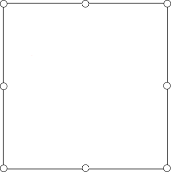
\includegraphics[interpolate=true,width=1.710000in,height=1.720000in]{graph/res/fisica_8sensores-img5.png}}%
\end{pgfscope}%
\begin{pgfscope}%
\definecolor{textcolor}{rgb}{0.000000,0.000000,0.000000}%
\pgfsetstrokecolor{textcolor}%
\pgfsetfillcolor{textcolor}%
\pgftext[x=4.203382in,y=3.956079in,,base]{\color{textcolor}\rmfamily\fontsize{12.000000}{14.400000}\selectfont Error en posición [cm]}%
\end{pgfscope}%
\begin{pgfscope}%
\pgfpathrectangle{\pgfqpoint{5.775845in}{1.127500in}}{\pgfqpoint{0.134750in}{2.695000in}}%
\pgfusepath{clip}%
\pgfsetbuttcap%
\pgfsetmiterjoin%
\definecolor{currentfill}{rgb}{1.000000,1.000000,1.000000}%
\pgfsetfillcolor{currentfill}%
\pgfsetlinewidth{0.010037pt}%
\definecolor{currentstroke}{rgb}{1.000000,1.000000,1.000000}%
\pgfsetstrokecolor{currentstroke}%
\pgfsetdash{}{0pt}%
\pgfpathmoveto{\pgfqpoint{5.775845in}{1.127500in}}%
\pgfpathlineto{\pgfqpoint{5.775845in}{1.138027in}}%
\pgfpathlineto{\pgfqpoint{5.775845in}{3.811973in}}%
\pgfpathlineto{\pgfqpoint{5.775845in}{3.822500in}}%
\pgfpathlineto{\pgfqpoint{5.910595in}{3.822500in}}%
\pgfpathlineto{\pgfqpoint{5.910595in}{3.811973in}}%
\pgfpathlineto{\pgfqpoint{5.910595in}{1.138027in}}%
\pgfpathlineto{\pgfqpoint{5.910595in}{1.127500in}}%
\pgfpathclose%
\pgfusepath{stroke,fill}%
\end{pgfscope}%
\begin{pgfscope}%
\pgfsys@transformshift{5.780000in}{1.130000in}%
\pgftext[left,bottom]{
\includegraphics[interpolate=true,width=0.130000in,height=2.690000in]{graph/res/fisica_8sensores-img6.png}}%
\end{pgfscope}%
\begin{pgfscope}%
\pgfsetbuttcap%
\pgfsetroundjoin%
\definecolor{currentfill}{rgb}{0.000000,0.000000,0.000000}%
\pgfsetfillcolor{currentfill}%
\pgfsetlinewidth{0.803000pt}%
\definecolor{currentstroke}{rgb}{0.000000,0.000000,0.000000}%
\pgfsetstrokecolor{currentstroke}%
\pgfsetdash{}{0pt}%
\pgfsys@defobject{currentmarker}{\pgfqpoint{0.000000in}{0.000000in}}{\pgfqpoint{0.048611in}{0.000000in}}{%
\pgfpathmoveto{\pgfqpoint{0.000000in}{0.000000in}}%
\pgfpathlineto{\pgfqpoint{0.048611in}{0.000000in}}%
\pgfusepath{stroke,fill}%
}%
\begin{pgfscope}%
\pgfsys@transformshift{5.910595in}{1.127500in}%
\pgfsys@useobject{currentmarker}{}%
\end{pgfscope}%
\end{pgfscope}%
\begin{pgfscope}%
\definecolor{textcolor}{rgb}{0.000000,0.000000,0.000000}%
\pgfsetstrokecolor{textcolor}%
\pgfsetfillcolor{textcolor}%
\pgftext[x=6.007818in, y=1.079672in, left, base]{\color{textcolor}\rmfamily\fontsize{10.000000}{12.000000}\selectfont \(\displaystyle {0}\)}%
\end{pgfscope}%
\begin{pgfscope}%
\pgfsetbuttcap%
\pgfsetroundjoin%
\definecolor{currentfill}{rgb}{0.000000,0.000000,0.000000}%
\pgfsetfillcolor{currentfill}%
\pgfsetlinewidth{0.803000pt}%
\definecolor{currentstroke}{rgb}{0.000000,0.000000,0.000000}%
\pgfsetstrokecolor{currentstroke}%
\pgfsetdash{}{0pt}%
\pgfsys@defobject{currentmarker}{\pgfqpoint{0.000000in}{0.000000in}}{\pgfqpoint{0.048611in}{0.000000in}}{%
\pgfpathmoveto{\pgfqpoint{0.000000in}{0.000000in}}%
\pgfpathlineto{\pgfqpoint{0.048611in}{0.000000in}}%
\pgfusepath{stroke,fill}%
}%
\begin{pgfscope}%
\pgfsys@transformshift{5.910595in}{1.613499in}%
\pgfsys@useobject{currentmarker}{}%
\end{pgfscope}%
\end{pgfscope}%
\begin{pgfscope}%
\definecolor{textcolor}{rgb}{0.000000,0.000000,0.000000}%
\pgfsetstrokecolor{textcolor}%
\pgfsetfillcolor{textcolor}%
\pgftext[x=6.007818in, y=1.565672in, left, base]{\color{textcolor}\rmfamily\fontsize{10.000000}{12.000000}\selectfont \(\displaystyle {10}\)}%
\end{pgfscope}%
\begin{pgfscope}%
\pgfsetbuttcap%
\pgfsetroundjoin%
\definecolor{currentfill}{rgb}{0.000000,0.000000,0.000000}%
\pgfsetfillcolor{currentfill}%
\pgfsetlinewidth{0.803000pt}%
\definecolor{currentstroke}{rgb}{0.000000,0.000000,0.000000}%
\pgfsetstrokecolor{currentstroke}%
\pgfsetdash{}{0pt}%
\pgfsys@defobject{currentmarker}{\pgfqpoint{0.000000in}{0.000000in}}{\pgfqpoint{0.048611in}{0.000000in}}{%
\pgfpathmoveto{\pgfqpoint{0.000000in}{0.000000in}}%
\pgfpathlineto{\pgfqpoint{0.048611in}{0.000000in}}%
\pgfusepath{stroke,fill}%
}%
\begin{pgfscope}%
\pgfsys@transformshift{5.910595in}{2.099499in}%
\pgfsys@useobject{currentmarker}{}%
\end{pgfscope}%
\end{pgfscope}%
\begin{pgfscope}%
\definecolor{textcolor}{rgb}{0.000000,0.000000,0.000000}%
\pgfsetstrokecolor{textcolor}%
\pgfsetfillcolor{textcolor}%
\pgftext[x=6.007818in, y=2.051671in, left, base]{\color{textcolor}\rmfamily\fontsize{10.000000}{12.000000}\selectfont \(\displaystyle {20}\)}%
\end{pgfscope}%
\begin{pgfscope}%
\pgfsetbuttcap%
\pgfsetroundjoin%
\definecolor{currentfill}{rgb}{0.000000,0.000000,0.000000}%
\pgfsetfillcolor{currentfill}%
\pgfsetlinewidth{0.803000pt}%
\definecolor{currentstroke}{rgb}{0.000000,0.000000,0.000000}%
\pgfsetstrokecolor{currentstroke}%
\pgfsetdash{}{0pt}%
\pgfsys@defobject{currentmarker}{\pgfqpoint{0.000000in}{0.000000in}}{\pgfqpoint{0.048611in}{0.000000in}}{%
\pgfpathmoveto{\pgfqpoint{0.000000in}{0.000000in}}%
\pgfpathlineto{\pgfqpoint{0.048611in}{0.000000in}}%
\pgfusepath{stroke,fill}%
}%
\begin{pgfscope}%
\pgfsys@transformshift{5.910595in}{2.585498in}%
\pgfsys@useobject{currentmarker}{}%
\end{pgfscope}%
\end{pgfscope}%
\begin{pgfscope}%
\definecolor{textcolor}{rgb}{0.000000,0.000000,0.000000}%
\pgfsetstrokecolor{textcolor}%
\pgfsetfillcolor{textcolor}%
\pgftext[x=6.007818in, y=2.537670in, left, base]{\color{textcolor}\rmfamily\fontsize{10.000000}{12.000000}\selectfont \(\displaystyle {30}\)}%
\end{pgfscope}%
\begin{pgfscope}%
\pgfsetbuttcap%
\pgfsetroundjoin%
\definecolor{currentfill}{rgb}{0.000000,0.000000,0.000000}%
\pgfsetfillcolor{currentfill}%
\pgfsetlinewidth{0.803000pt}%
\definecolor{currentstroke}{rgb}{0.000000,0.000000,0.000000}%
\pgfsetstrokecolor{currentstroke}%
\pgfsetdash{}{0pt}%
\pgfsys@defobject{currentmarker}{\pgfqpoint{0.000000in}{0.000000in}}{\pgfqpoint{0.048611in}{0.000000in}}{%
\pgfpathmoveto{\pgfqpoint{0.000000in}{0.000000in}}%
\pgfpathlineto{\pgfqpoint{0.048611in}{0.000000in}}%
\pgfusepath{stroke,fill}%
}%
\begin{pgfscope}%
\pgfsys@transformshift{5.910595in}{3.071497in}%
\pgfsys@useobject{currentmarker}{}%
\end{pgfscope}%
\end{pgfscope}%
\begin{pgfscope}%
\definecolor{textcolor}{rgb}{0.000000,0.000000,0.000000}%
\pgfsetstrokecolor{textcolor}%
\pgfsetfillcolor{textcolor}%
\pgftext[x=6.007818in, y=3.023670in, left, base]{\color{textcolor}\rmfamily\fontsize{10.000000}{12.000000}\selectfont \(\displaystyle {40}\)}%
\end{pgfscope}%
\begin{pgfscope}%
\pgfsetbuttcap%
\pgfsetroundjoin%
\definecolor{currentfill}{rgb}{0.000000,0.000000,0.000000}%
\pgfsetfillcolor{currentfill}%
\pgfsetlinewidth{0.803000pt}%
\definecolor{currentstroke}{rgb}{0.000000,0.000000,0.000000}%
\pgfsetstrokecolor{currentstroke}%
\pgfsetdash{}{0pt}%
\pgfsys@defobject{currentmarker}{\pgfqpoint{0.000000in}{0.000000in}}{\pgfqpoint{0.048611in}{0.000000in}}{%
\pgfpathmoveto{\pgfqpoint{0.000000in}{0.000000in}}%
\pgfpathlineto{\pgfqpoint{0.048611in}{0.000000in}}%
\pgfusepath{stroke,fill}%
}%
\begin{pgfscope}%
\pgfsys@transformshift{5.910595in}{3.557497in}%
\pgfsys@useobject{currentmarker}{}%
\end{pgfscope}%
\end{pgfscope}%
\begin{pgfscope}%
\definecolor{textcolor}{rgb}{0.000000,0.000000,0.000000}%
\pgfsetstrokecolor{textcolor}%
\pgfsetfillcolor{textcolor}%
\pgftext[x=6.007818in, y=3.509669in, left, base]{\color{textcolor}\rmfamily\fontsize{10.000000}{12.000000}\selectfont \(\displaystyle {50}\)}%
\end{pgfscope}%
\begin{pgfscope}%
\definecolor{textcolor}{rgb}{0.000000,0.000000,0.000000}%
\pgfsetstrokecolor{textcolor}%
\pgfsetfillcolor{textcolor}%
\pgftext[x=6.355040in,y=2.475000in,,top,rotate=270.000000]{\color{textcolor}\rmfamily\fontsize{10.000000}{12.000000}\selectfont Diferencia de posición [cm]}%
\end{pgfscope}%
\begin{pgfscope}%
\pgfsetbuttcap%
\pgfsetmiterjoin%
\pgfsetlinewidth{0.803000pt}%
\definecolor{currentstroke}{rgb}{0.000000,0.000000,0.000000}%
\pgfsetstrokecolor{currentstroke}%
\pgfsetdash{}{0pt}%
\pgfpathmoveto{\pgfqpoint{5.775845in}{1.127500in}}%
\pgfpathlineto{\pgfqpoint{5.775845in}{1.138027in}}%
\pgfpathlineto{\pgfqpoint{5.775845in}{3.811973in}}%
\pgfpathlineto{\pgfqpoint{5.775845in}{3.822500in}}%
\pgfpathlineto{\pgfqpoint{5.910595in}{3.822500in}}%
\pgfpathlineto{\pgfqpoint{5.910595in}{3.811973in}}%
\pgfpathlineto{\pgfqpoint{5.910595in}{1.138027in}}%
\pgfpathlineto{\pgfqpoint{5.910595in}{1.127500in}}%
\pgfpathclose%
\pgfusepath{stroke}%
\end{pgfscope}%
\begin{pgfscope}%
\pgfpathrectangle{\pgfqpoint{0.263486in}{1.323551in}}{\pgfqpoint{0.122303in}{2.446055in}}%
\pgfusepath{clip}%
\pgfsetbuttcap%
\pgfsetmiterjoin%
\definecolor{currentfill}{rgb}{1.000000,1.000000,1.000000}%
\pgfsetfillcolor{currentfill}%
\pgfsetlinewidth{0.010037pt}%
\definecolor{currentstroke}{rgb}{1.000000,1.000000,1.000000}%
\pgfsetstrokecolor{currentstroke}%
\pgfsetdash{}{0pt}%
\pgfpathmoveto{\pgfqpoint{0.263486in}{1.323551in}}%
\pgfpathlineto{\pgfqpoint{0.263486in}{1.333106in}}%
\pgfpathlineto{\pgfqpoint{0.263486in}{3.760051in}}%
\pgfpathlineto{\pgfqpoint{0.263486in}{3.769605in}}%
\pgfpathlineto{\pgfqpoint{0.385789in}{3.769605in}}%
\pgfpathlineto{\pgfqpoint{0.385789in}{3.760051in}}%
\pgfpathlineto{\pgfqpoint{0.385789in}{1.333106in}}%
\pgfpathlineto{\pgfqpoint{0.385789in}{1.323551in}}%
\pgfpathclose%
\pgfusepath{stroke,fill}%
\end{pgfscope}%
\begin{pgfscope}%
\pgfsys@transformshift{0.260000in}{1.320000in}%
\pgftext[left,bottom]{
\includegraphics[interpolate=true,width=0.130000in,height=2.450000in]{graph/res/fisica_8sensores-img7.png}}%
\end{pgfscope}%
\begin{pgfscope}%
\pgfsetbuttcap%
\pgfsetroundjoin%
\definecolor{currentfill}{rgb}{0.000000,0.000000,0.000000}%
\pgfsetfillcolor{currentfill}%
\pgfsetlinewidth{0.803000pt}%
\definecolor{currentstroke}{rgb}{0.000000,0.000000,0.000000}%
\pgfsetstrokecolor{currentstroke}%
\pgfsetdash{}{0pt}%
\pgfsys@defobject{currentmarker}{\pgfqpoint{0.000000in}{0.000000in}}{\pgfqpoint{0.048611in}{0.000000in}}{%
\pgfpathmoveto{\pgfqpoint{0.000000in}{0.000000in}}%
\pgfpathlineto{\pgfqpoint{0.048611in}{0.000000in}}%
\pgfusepath{stroke,fill}%
}%
\begin{pgfscope}%
\pgfsys@transformshift{0.385789in}{1.340315in}%
\pgfsys@useobject{currentmarker}{}%
\end{pgfscope}%
\end{pgfscope}%
\begin{pgfscope}%
\definecolor{textcolor}{rgb}{0.000000,0.000000,0.000000}%
\pgfsetstrokecolor{textcolor}%
\pgfsetfillcolor{textcolor}%
\pgftext[x=0.483011in, y=1.292487in, left, base]{\color{textcolor}\rmfamily\fontsize{10.000000}{12.000000}\selectfont \(\displaystyle {−30}\)}%
\end{pgfscope}%
\begin{pgfscope}%
\pgfsetbuttcap%
\pgfsetroundjoin%
\definecolor{currentfill}{rgb}{0.000000,0.000000,0.000000}%
\pgfsetfillcolor{currentfill}%
\pgfsetlinewidth{0.803000pt}%
\definecolor{currentstroke}{rgb}{0.000000,0.000000,0.000000}%
\pgfsetstrokecolor{currentstroke}%
\pgfsetdash{}{0pt}%
\pgfsys@defobject{currentmarker}{\pgfqpoint{0.000000in}{0.000000in}}{\pgfqpoint{0.048611in}{0.000000in}}{%
\pgfpathmoveto{\pgfqpoint{0.000000in}{0.000000in}}%
\pgfpathlineto{\pgfqpoint{0.048611in}{0.000000in}}%
\pgfusepath{stroke,fill}%
}%
\begin{pgfscope}%
\pgfsys@transformshift{0.385789in}{1.648186in}%
\pgfsys@useobject{currentmarker}{}%
\end{pgfscope}%
\end{pgfscope}%
\begin{pgfscope}%
\definecolor{textcolor}{rgb}{0.000000,0.000000,0.000000}%
\pgfsetstrokecolor{textcolor}%
\pgfsetfillcolor{textcolor}%
\pgftext[x=0.483011in, y=1.600358in, left, base]{\color{textcolor}\rmfamily\fontsize{10.000000}{12.000000}\selectfont \(\displaystyle {−20}\)}%
\end{pgfscope}%
\begin{pgfscope}%
\pgfsetbuttcap%
\pgfsetroundjoin%
\definecolor{currentfill}{rgb}{0.000000,0.000000,0.000000}%
\pgfsetfillcolor{currentfill}%
\pgfsetlinewidth{0.803000pt}%
\definecolor{currentstroke}{rgb}{0.000000,0.000000,0.000000}%
\pgfsetstrokecolor{currentstroke}%
\pgfsetdash{}{0pt}%
\pgfsys@defobject{currentmarker}{\pgfqpoint{0.000000in}{0.000000in}}{\pgfqpoint{0.048611in}{0.000000in}}{%
\pgfpathmoveto{\pgfqpoint{0.000000in}{0.000000in}}%
\pgfpathlineto{\pgfqpoint{0.048611in}{0.000000in}}%
\pgfusepath{stroke,fill}%
}%
\begin{pgfscope}%
\pgfsys@transformshift{0.385789in}{1.956056in}%
\pgfsys@useobject{currentmarker}{}%
\end{pgfscope}%
\end{pgfscope}%
\begin{pgfscope}%
\definecolor{textcolor}{rgb}{0.000000,0.000000,0.000000}%
\pgfsetstrokecolor{textcolor}%
\pgfsetfillcolor{textcolor}%
\pgftext[x=0.483011in, y=1.908229in, left, base]{\color{textcolor}\rmfamily\fontsize{10.000000}{12.000000}\selectfont \(\displaystyle {−10}\)}%
\end{pgfscope}%
\begin{pgfscope}%
\pgfsetbuttcap%
\pgfsetroundjoin%
\definecolor{currentfill}{rgb}{0.000000,0.000000,0.000000}%
\pgfsetfillcolor{currentfill}%
\pgfsetlinewidth{0.803000pt}%
\definecolor{currentstroke}{rgb}{0.000000,0.000000,0.000000}%
\pgfsetstrokecolor{currentstroke}%
\pgfsetdash{}{0pt}%
\pgfsys@defobject{currentmarker}{\pgfqpoint{0.000000in}{0.000000in}}{\pgfqpoint{0.048611in}{0.000000in}}{%
\pgfpathmoveto{\pgfqpoint{0.000000in}{0.000000in}}%
\pgfpathlineto{\pgfqpoint{0.048611in}{0.000000in}}%
\pgfusepath{stroke,fill}%
}%
\begin{pgfscope}%
\pgfsys@transformshift{0.385789in}{2.263927in}%
\pgfsys@useobject{currentmarker}{}%
\end{pgfscope}%
\end{pgfscope}%
\begin{pgfscope}%
\definecolor{textcolor}{rgb}{0.000000,0.000000,0.000000}%
\pgfsetstrokecolor{textcolor}%
\pgfsetfillcolor{textcolor}%
\pgftext[x=0.483011in, y=2.216099in, left, base]{\color{textcolor}\rmfamily\fontsize{10.000000}{12.000000}\selectfont \(\displaystyle {0}\)}%
\end{pgfscope}%
\begin{pgfscope}%
\pgfsetbuttcap%
\pgfsetroundjoin%
\definecolor{currentfill}{rgb}{0.000000,0.000000,0.000000}%
\pgfsetfillcolor{currentfill}%
\pgfsetlinewidth{0.803000pt}%
\definecolor{currentstroke}{rgb}{0.000000,0.000000,0.000000}%
\pgfsetstrokecolor{currentstroke}%
\pgfsetdash{}{0pt}%
\pgfsys@defobject{currentmarker}{\pgfqpoint{0.000000in}{0.000000in}}{\pgfqpoint{0.048611in}{0.000000in}}{%
\pgfpathmoveto{\pgfqpoint{0.000000in}{0.000000in}}%
\pgfpathlineto{\pgfqpoint{0.048611in}{0.000000in}}%
\pgfusepath{stroke,fill}%
}%
\begin{pgfscope}%
\pgfsys@transformshift{0.385789in}{2.571798in}%
\pgfsys@useobject{currentmarker}{}%
\end{pgfscope}%
\end{pgfscope}%
\begin{pgfscope}%
\definecolor{textcolor}{rgb}{0.000000,0.000000,0.000000}%
\pgfsetstrokecolor{textcolor}%
\pgfsetfillcolor{textcolor}%
\pgftext[x=0.483011in, y=2.523970in, left, base]{\color{textcolor}\rmfamily\fontsize{10.000000}{12.000000}\selectfont \(\displaystyle {10}\)}%
\end{pgfscope}%
\begin{pgfscope}%
\pgfsetbuttcap%
\pgfsetroundjoin%
\definecolor{currentfill}{rgb}{0.000000,0.000000,0.000000}%
\pgfsetfillcolor{currentfill}%
\pgfsetlinewidth{0.803000pt}%
\definecolor{currentstroke}{rgb}{0.000000,0.000000,0.000000}%
\pgfsetstrokecolor{currentstroke}%
\pgfsetdash{}{0pt}%
\pgfsys@defobject{currentmarker}{\pgfqpoint{0.000000in}{0.000000in}}{\pgfqpoint{0.048611in}{0.000000in}}{%
\pgfpathmoveto{\pgfqpoint{0.000000in}{0.000000in}}%
\pgfpathlineto{\pgfqpoint{0.048611in}{0.000000in}}%
\pgfusepath{stroke,fill}%
}%
\begin{pgfscope}%
\pgfsys@transformshift{0.385789in}{2.879668in}%
\pgfsys@useobject{currentmarker}{}%
\end{pgfscope}%
\end{pgfscope}%
\begin{pgfscope}%
\definecolor{textcolor}{rgb}{0.000000,0.000000,0.000000}%
\pgfsetstrokecolor{textcolor}%
\pgfsetfillcolor{textcolor}%
\pgftext[x=0.483011in, y=2.831841in, left, base]{\color{textcolor}\rmfamily\fontsize{10.000000}{12.000000}\selectfont \(\displaystyle {20}\)}%
\end{pgfscope}%
\begin{pgfscope}%
\pgfsetbuttcap%
\pgfsetroundjoin%
\definecolor{currentfill}{rgb}{0.000000,0.000000,0.000000}%
\pgfsetfillcolor{currentfill}%
\pgfsetlinewidth{0.803000pt}%
\definecolor{currentstroke}{rgb}{0.000000,0.000000,0.000000}%
\pgfsetstrokecolor{currentstroke}%
\pgfsetdash{}{0pt}%
\pgfsys@defobject{currentmarker}{\pgfqpoint{0.000000in}{0.000000in}}{\pgfqpoint{0.048611in}{0.000000in}}{%
\pgfpathmoveto{\pgfqpoint{0.000000in}{0.000000in}}%
\pgfpathlineto{\pgfqpoint{0.048611in}{0.000000in}}%
\pgfusepath{stroke,fill}%
}%
\begin{pgfscope}%
\pgfsys@transformshift{0.385789in}{3.187539in}%
\pgfsys@useobject{currentmarker}{}%
\end{pgfscope}%
\end{pgfscope}%
\begin{pgfscope}%
\definecolor{textcolor}{rgb}{0.000000,0.000000,0.000000}%
\pgfsetstrokecolor{textcolor}%
\pgfsetfillcolor{textcolor}%
\pgftext[x=0.483011in, y=3.139711in, left, base]{\color{textcolor}\rmfamily\fontsize{10.000000}{12.000000}\selectfont \(\displaystyle {30}\)}%
\end{pgfscope}%
\begin{pgfscope}%
\pgfsetbuttcap%
\pgfsetroundjoin%
\definecolor{currentfill}{rgb}{0.000000,0.000000,0.000000}%
\pgfsetfillcolor{currentfill}%
\pgfsetlinewidth{0.803000pt}%
\definecolor{currentstroke}{rgb}{0.000000,0.000000,0.000000}%
\pgfsetstrokecolor{currentstroke}%
\pgfsetdash{}{0pt}%
\pgfsys@defobject{currentmarker}{\pgfqpoint{0.000000in}{0.000000in}}{\pgfqpoint{0.048611in}{0.000000in}}{%
\pgfpathmoveto{\pgfqpoint{0.000000in}{0.000000in}}%
\pgfpathlineto{\pgfqpoint{0.048611in}{0.000000in}}%
\pgfusepath{stroke,fill}%
}%
\begin{pgfscope}%
\pgfsys@transformshift{0.385789in}{3.495410in}%
\pgfsys@useobject{currentmarker}{}%
\end{pgfscope}%
\end{pgfscope}%
\begin{pgfscope}%
\definecolor{textcolor}{rgb}{0.000000,0.000000,0.000000}%
\pgfsetstrokecolor{textcolor}%
\pgfsetfillcolor{textcolor}%
\pgftext[x=0.483011in, y=3.447582in, left, base]{\color{textcolor}\rmfamily\fontsize{10.000000}{12.000000}\selectfont \(\displaystyle {40}\)}%
\end{pgfscope}%
\begin{pgfscope}%
\definecolor{textcolor}{rgb}{0.000000,0.000000,0.000000}%
\pgfsetstrokecolor{textcolor}%
\pgfsetfillcolor{textcolor}%
\pgftext[x=0.035481in,y=2.546578in,,top,rotate=90.000000]{\color{textcolor}\rmfamily\fontsize{10.000000}{12.000000}\selectfont Diferencia en la medida de cada eje [cm]}%
\end{pgfscope}%
\begin{pgfscope}%
\pgfsetbuttcap%
\pgfsetmiterjoin%
\pgfsetlinewidth{0.803000pt}%
\definecolor{currentstroke}{rgb}{0.000000,0.000000,0.000000}%
\pgfsetstrokecolor{currentstroke}%
\pgfsetdash{}{0pt}%
\pgfpathmoveto{\pgfqpoint{0.263486in}{1.323551in}}%
\pgfpathlineto{\pgfqpoint{0.263486in}{1.333106in}}%
\pgfpathlineto{\pgfqpoint{0.263486in}{3.760051in}}%
\pgfpathlineto{\pgfqpoint{0.263486in}{3.769605in}}%
\pgfpathlineto{\pgfqpoint{0.385789in}{3.769605in}}%
\pgfpathlineto{\pgfqpoint{0.385789in}{3.760051in}}%
\pgfpathlineto{\pgfqpoint{0.385789in}{1.333106in}}%
\pgfpathlineto{\pgfqpoint{0.385789in}{1.323551in}}%
\pgfpathclose%
\pgfusepath{stroke}%
\end{pgfscope}%
\end{pgfpicture}%
\makeatother%
\endgroup%

    \caption{Resultados de las medidas en el edificio de Física con 8 balizas. Entre paréntesis se indica la desviación estándar de los errores obtenidos en cada punto.}
    \label{fig:res_fisica_8}
\end{figure}

En este caso es posible observar una mejora generalizada tanto en valores de discrepancia como en sus desviaciones, salvo en el punto 4.
Tras revisar los datos en busca de la fuente de este error se comprobó que fue debido a un fallo en el posicionamiento de los sensores, no del posicionamiento local del robot.
La posición que proporcionaron dio en el eje $y$ un valor que colocaría al robot fuera de la planta.

Este hecho se repite a lo largo de las tres medidas realizadas, aunque con distintos valores --de ahí también el alto valor en la desviación estándar de las medidas en el punto--, por lo que es probable que se trate de un caso en el que la tercera baliza utilizada --en dos de ellas se tenía una visión directa-- se haya visto ocultada por una de las columnas.

\begin{table}[H]
  \hspace*{-0.5cm}
  \centering
  \begin{tabular}{c|c|c|c|c|c|}
    \cline{2-6}
                                              & \begin{tabular}[c]{@{}c@{}}Error en \\ eje $x$ (cm) \end{tabular} & \begin{tabular}[c]{@{}c@{}} Error en \\ eje $y$ (cm) \end{tabular} & \begin{tabular}[c]{@{}c@{}} Error en eje $x$ \\ (absoluto) (cm) \end{tabular} & \begin{tabular}[c]{@{}c@{}} Error en eje $y$ \\ (absoluto) (cm) \end{tabular} & \begin{tabular}[c]{@{}c@{}} Error en \\ posición(cm) \end{tabular}\\ \hline
    \multicolumn{1}{|c|}{Media}               &  -3.5   &  -6.2   &      11.9          &         13.7       &  22.3    \\ \hline
    \multicolumn{1}{|c|}{Mediana}             &  -4.7   &  -7.1   &      11.4          &         9.6        &  19.1    \\ \hline
    \multicolumn{1}{|c|}{Desv. estándar} &  13.6   &   12.3  &      7.5           &         12.3       &  12.2    \\ \hline
    \multicolumn{1}{|c|}{Máximo}              &  21.0   &   48.9  &      25.8          &         48.9       &  55.5    \\ \hline
    \multicolumn{1}{|c|}{Mínimo}              &  -40.7  &  -30.5  &      3.3           &         1.5        &  5.6     \\ \hline
\end{tabular}
\caption{Resumen de los errores en el edificio de Física con 8 balizas.}
\label{tab:media_fisica_8}
\end{table}

Los valores medios recogidos en la Tabla \ref{tab:media_fisica_8}, debido al número bajo de datos, se ven claramente influenciados por los valores anormalmente altos del punto 4, también con una desviación estándar más alta que en el caso de 6 balizas.
La diferencia entre media y mediana lo muestra, aunque ambos valores son los mejores obtenidos en el edificio de Física.

\begin{figure}[H]
  \centering
    \begin{subfigure}[b]{.3\textwidth}
      \centering
      \hspace*{-0.8cm}
      \begin{tikzpicture}
    \begin{axis}[
        ylabel = {Error[cm]},
        x = 0.25\textwidth,
        boxplot/draw direction=y,
        ymajorgrids,
        xtick={1,2,3},
        xticklabels={4 bal., 6 bal., 8 bal.},
        ]
        \addplot+ [boxplot] table[y index=0] {data/4sens_fisica.txt};
        \addplot+ [boxplot] table[y index=0] {data/6sens_fisica.txt};
        \addplot+ [boxplot] table[y index=0] {data/8sens_fisica.txt};
    \end{axis}
\end{tikzpicture} 
      % \vspace*{-0.5cm}
      \caption{Eje x}
      \label{fig:boxplot_fisica_x}
    \end{subfigure}
    \hspace*{0.1cm}
    \begin{subfigure}[b]{.3\textwidth}
      \centering
      \begin{tikzpicture}
    \begin{axis}[
        x = 0.25\textwidth,
        boxplot/draw direction=y,
        ymajorgrids,
        xtick={1,2,3},
        xticklabels={4 bal., 6 bal., 8 bal.},
        ]
        \addplot+ [boxplot] table[y index=1] {data/4sens_fisica.txt};
        \addplot+ [boxplot] table[y index=1] {data/6sens_fisica.txt};
        \addplot+ [boxplot] table[y index=1] {data/8sens_fisica.txt};
    \end{axis}
\end{tikzpicture}  
      % \vspace*{-0.5cm}
      \caption{Eje y}
      \label{fig:boxplot_fisica_y}
    \end{subfigure}
    ~~~~
    \begin{subfigure}[b]{.3\textwidth}
        \centering
        \begin{tikzpicture}
    \begin{axis}[
        x = 0.25\textwidth,
        boxplot/draw direction=y,
        ymajorgrids,
        xtick={1,2,3},
        xticklabels={4 bal., 6 bal., 8 bal.},
        ]
        \addplot+ [boxplot] table[y index=2] {data/4sens_fisica.txt};
        \addplot+ [boxplot] table[y index=2] {data/6sens_fisica.txt};
        \addplot+ [boxplot] table[y index=2] {data/8sens_fisica.txt};
    \end{axis}
\end{tikzpicture}  
        \caption{Posición}
        \label{fig:boxplot_fisica_pos}
      \end{subfigure}
    \caption{Comparación del rendimiento de las configuraciones de balizas en el edificio de Física.}
    \label{fig:boxplot_fisica}
\end{figure}

Los diagramas de cajas de la Figura~\ref{fig:boxplot_fisica} muestran unos resultados similares a los obtenidos en el laboratorio: un número mayor de balizas resulta en unos valores más bajos de error en el posicionamiento del objetivo.

Además, confirma la conclusión expuesta en la comparación de aquellos resultados: debido a la utilización de 4 balizas en todo momento del kit, independientemente del número de balizas configuradas en total, la posición en la que se colocan es crítica.

Es posible observar este hecho en los diagramas de cada eje.
En la configuración con 6 balizas se añadieron en los extremos del eje $y$, y es en dicho eje donde se observan unas mejoras en mayor medida, a pesar de que, como se ha comentado, una de las balizas tuviera una colocación mejorable.

El mismo fenómeno se da en el caso del empleo de 8 balizas, donde la colocación de balizas adicionales en los extremos del eje $x$ proporciona unos valores con una dispersión mucho menor en este eje.

Aunque los resultados en este escenario no ideal son, como era de esperar, peores que en el ideal, la diferencia relativa en el caso de 4 balizas es del $23.4$ \% para los valores medios y $18.9$ \% para las desviaciones estándar del posicionamiento, que equivalen a unos pocos centímetros.
Estas diferencias se deben principalmente a la mayor distancia entre balizas y objetivo, y no tanto a la presencia de obstáculos.
La anchura de las columnas no parece ser suficiente para evitar la línea de visión directa entre las balizas y el objetivo de forma general, aunque sí que es posible apreciar su efecto puntualmente, como en el caso del uso de 8 balizas, dando en uno de los puntos un resultado muy alejado de la media.

La diferencia en los casos con 6 balizas es similar, con una diferencia relativa en los valores medios del $18.9$ \% y del $44.4$ \% para las desviaciones estándar del error en el posicionamiento, de nuevo achacables a la mayor distancia entre balizas y objetivo.

% Al igual que en el primer escenario, la adición de nuevas balizas fue distribuida de tal forma que el objetivo pueda encontrar, de media, distancias menores respecto a cada una de ellas, obteniendo mejoras más discretas en los puntos donde esto no ocurre.

%------------------------------------------------------------------------------
%                             Conclusiones
%------------------------------------------------------------------------------

\newpage
\section{Conclusiones}

Para determinar la precisión en el posicionamiento de un kit de sensores de Ultra-wide Band se ha procedido a tomar varias medidas con la ayuda de un robot capaz de desplazarse de forma autónoma en dos escenarios, uno libre de objetos y un segundo con una superficie mayor y con obstáculos que pudieran impedir en ciertas ocasiones el correcto desempeño del posicionamiento del kit utilizado.

Además de las distintas localizaciones, en cada uno de los dos escenarios se han recogido datos con distintas configuraciones de balizas, de tal forma que ha sido posible determinar el efecto de su colocación en el posicionamiento del objetivo.

Las medidas en los dos escenarios han arrojado resultados similares: una distribución uniforme de balizas proporciona mejores resultados fruto de dar opción al kit de utilizar sensores más cercanos para el posicionamiento del objetivo.

Así, para maximizar el rendimiento de este kit no solo se deberán usar un número mayor de balizas, si no que será necesario un estudio que permita obtener una configuración en la zona de interés tal que los objetivos a posicionar se encuentren a la menor distancia posible de al menos 4 balizas.

En ninguno de los dos escenarios contemplados en este trabajo se han obtenido valores medios de error en el posicionamiento mayores a 30cm, teniendo en cuenta además que en todos ellos, además del error de precisión dado por la tecnología de UWB, se añadía el posible error de posicionamiento del robot.
Es decir, es posible encontrar en superficies del orden de decenas de metros cuadrados, errores medios de, al menos, dos órdenes de magnitud menores.

Estos resultados abren la puerta a su empleo en el posicionamiento de robots teniendo en cuenta que dicho error entrará en la mayoría de casos en sus propias dimensiones o con humanos, siendo 30cm apenas dar un paso.

En superficies aún mayores que las tratadas se deberían obtener unos resultados parecidos siempre con una colocación de un número mayor de balizas respetando las condiciones de homogeneidad en las distancias ya discutida.

Aun así, el problema del posicionamiento local no está completamente resuelto.
Los resultados expuestos en este trabajo son valores medios obtenidos a partir de numerosas medidas de un kit de UWB, pero en algunas de las aplicaciones donde se necesite realizar el posicionamiento de forma veloz la naturaleza aleatoria de las señales empleadas pueden provocar un pobre rendimiento de estas técnicas.

Obstáculos dinámicos también juegan un gran papel en la precisión del posicionamiento local.
En el caso del UWB la visión directa entre los sensores es crítica para su correcto funcionamiento y la posición de las balizas debe contemplarla, por lo que escenarios con obstáculos impredecibles evitarán su correcto funcionamiento.

La proliferación de la tecnología UWB da una nueva alternativa a los sistemas de posicionamiento local ya establecidos y discutidos en este trabajo.
Tratando de evitar en la medida de lo posible los casos donde aparecen sus puntos débiles, proporciona una precisión y robustez muy superior a sus alternativas, por lo que se presenta en estos momentos como una de la mejores opciones en este ámbito.

%------------------------------------------------------------------------------
%                             Bibliografía
%------------------------------------------------------------------------------

\newpage
\section{Bibliografía}

\begingroup
    \renewcommand{\section}[2]{}%
    \bibliography{refs} 
    \bibliographystyle{ieeetr}
\endgroup


%------------------------------------------------------------------------------
%                             Apéndices
%------------------------------------------------------------------------------

\newpage
\section*{Apéndice A}
\renewcommand{\thetable}{A.\arabic{table}}
\setcounter{table}{0}

\subsection{Medidas en el laboratorio de Robótica del ICCAEx}
% En todas las tablas de este apéndice, los puntos están referidos de acuerdo a la disposición de la Figura \ref{fig:puntos}.

\subsubsection{Medidas con 4 balizas}
\begin{table}[H]
    \centering
    % \hspace*{-1.4cm}
    \begin{tabular}{|c|c|c|c|c|c|c|}
        \hline
        \multirow{2}{*}{Punto} & \multicolumn{2}{c|}{Error en eje $x$ [cm]} & \multicolumn{2}{c|}{Error en eje $y$ [cm]} & \multicolumn{2}{c|}{Error en posición [cm]} \\ \cline{2-7} 
        & \begin{tabular}[c]{@{}c@{}}Valor\\ medio\end{tabular} & \begin{tabular}[c]{@{}c@{}}Desviación\\ estándar\end{tabular} & \begin{tabular}[c]{@{}c@{}}Valor\\ medio\end{tabular} & \begin{tabular}[c]{@{}c@{}}Desviación\\ estándar\end{tabular} & \begin{tabular}[c]{@{}c@{}}Valor\\ medio\end{tabular} & \begin{tabular}[c]{@{}c@{}}Desviación\\ estándar\end{tabular} \\ \hline
        1    &  $-3.34$   &  $7.01$   &   $3.05$    &   $4.27$  &  $10.17$  & $1.14$\\ \hline
        2    &  $-1.86$   &  $4.18$   &   $3.81$    &   $0.56$  &  $8.36$   & $0.64$        \\ \hline
        3    &  $-1.15$   &  $1.62$   &   $6.23$    &   $4.60$  &  $7.21$   & $4.45$        \\ \hline
        4    &  $-10.54$  &  $6.32$   &   $7.90$    &   $1.02$  &  $19.01$  & $7.72$  \\ \hline
        5    &  $-3.02$   &  $14.44$  &   $5.38$    &   $2.51$  &  $15.72$  & $3.91$   \\ \hline
        6    &  $1.13$    &  $13.95$  &   $3.88$    &   $1.40$  &  $14.17$  & $4.81$   \\ \hline
        7    &  $13.74$   &  $10.62$  &   $7.81$    &   $4.45$  &  $17.39$  & $9.28$   \\ \hline
        8    &  $13.13$   &  $8.71$   &   $0.81$    &   $0.80$  &  $15.82$  & $5.54$   \\ \hline
        9    &  $10.46$   &  $7.18$   &   $4.16$    &   $2.82$  &  $14.96$  & $3.46$   \\ \hline
        10   &  $20.06$   &  $7.80$   &   $10.14$   &   $4.09$  &  $23.83$  & $5.24$   \\ \hline
        11   &  $-6.46$   &  $13.53$  &   $-7.72$   &   $4.90$  &  $17.85$  & $3.31$   \\ \hline
        12   &  $9.53$    &  $8.38$   &   $7.00$    &   $2.06$  &  $13.40$  & $6.89$   \\ \hline
        13   &  $16.21$   &  $2.61$   &   $4.09$    &   $3.91$  &  $18.10$  & $1.44$   \\ \hline
        14   &  $16.48$   &  $7.87$   &   $2.04$    &   $3.47$  &  $17.70$  & $7.44$   \\ \hline
        15   &  $19.82$   &  $6.56$   &   $3.28$    &   $2.61$  &  $21.02$  & $5.55$   \\ \hline
        16   &  $0.97$    &  $5.73$   &   $-3.62$   &   $4.71$  &  $12.99$  & $6.01$   \\ \hline
        17   &  $-4.32$   &  $9.59$   &   $4.44$    &   $6.48$  &  $17.51$  & $2.44$   \\ \hline
        18   &  $-3.54$   &  $7.69$   &   $0.93$    &   $0.61$  &  $11.54$  & $5.05$   \\ \hline
        19   &  $0.55$    &  $6.68$   &   $2.42$    &   $3.69$  &  $9.43$   & $1.20$   \\ \hline
        20   &  $4.41$    &  $6.45$   &   $4.58$    &   $5.20$  &  $11.21$  & $2.39$   \\ \hline
        21   &  $-22.66$  &  $10.77$  &   $-2.74$   &   $9.29$  &  $25.75$  & $8.24$   \\ \hline
        22   &  $-23.33$  &  $10.62$  &   $-7.30$   &   $1.17$  &  $24.92$  & $10.19$  \\ \hline
        23   &  $-13.40$  &  $5.05$   &   $4.93$    &   $4.44$  &  $15.31$  & $5.32$   \\ \hline
        24   &  $-2.70$   &  $7.63$   &   $5.93$    &   $4.94$  &  $13.13$  & $5.09$   \\ \hline
        25   &  $11.06$   &  $8.65$   &   $10.84$   &   $3.29$  &  $18.34$  & $2.86$   \\ \hline
        26   &  $-20.22$  &  $9.67$   &   $5.91$    &   $9.25$  &  $22.67$  & $11.93$  \\ \hline
        27   &  $-25.63$  &  $7.46$   &   $-12.45$  &   $3.00$  &  $29.18$  & $5.79$   \\ \hline
        28   &  $-24.55$  &  $10.38$  &   $-2.28$   &   $6.19$  &  $25.87$  & $9.98$   \\ \hline
        29   &  $-25.92$  &  $6.64$   &   $0.69$    &   $3.35$  &  $27.10$  & $6.05$   \\ \hline
        30   &  $-5.83$   &  $7.97$   &   $14.42$   &   $1.77$  &  $17.16$  & $5.01$   \\ \hline
        31   &  $-28.22$  &  $1.59$   &   $-4.31$   &   $2.22$  &  $29.57$  & $1.94$   \\ \hline
        32   &  $-30.45$  &  $3.22$   &   $-6.87$   &   $2.63$  &  $31.36$  & $3.69$   \\ \hline
        33   &  $-37.37$  &  $11.18$  &   $8.23$    &   $6.68$  &  $38.86$  & $12.58$  \\ \hline
        34   &  $-56.61$  &  $2.56$   &   $9.84$    &   $0.47$  &  $57.65$  & $2.38$   \\ \hline
        35   &  $-22.70$  &  $1.35$   &   $12.11$   &   $2.80$  &  $26.90$  & $0.03$   \\ \hline
    \end{tabular}
    \caption{Valor medio y desviación estándar de los errores para cada eje y para el posicionamiento en cada punto para el conjunto de trayectorias con 4 balizas.}
    \label{tab:media_lab_4_total}
\end{table}

\newpage
\subsubsection{Medidas de cada trayectoria con 4 balizas}

\begin{table}[H]
    \centering
    \begin{tabular}{|c|c|c|c|c|c|c|}
        \hline
        \multirow{2}{*}{Punto} & \multicolumn{2}{c|}{Error en eje $x$ [cm]} & \multicolumn{2}{c|}{Error en eje $y$ [cm]} & \multicolumn{2}{c|}{Error en posición [cm]} \\ \cline{2-7} 
        & \begin{tabular}[c]{@{}c@{}}Valor\\ medio\end{tabular} & \begin{tabular}[c]{@{}c@{}}Desviación\\ estándar\end{tabular} & \begin{tabular}[c]{@{}c@{}}Valor\\ medio\end{tabular} & \begin{tabular}[c]{@{}c@{}}Desviación\\ estándar\end{tabular} & \begin{tabular}[c]{@{}c@{}}Valor\\ medio\end{tabular} & \begin{tabular}[c]{@{}c@{}}Desviación\\ estándar\end{tabular} \\ \hline
        1   &    $3.67$    &  $5.51$  & $7.32$   &  $2.80$  & $9.03$   &  $4.87$  \\ \hline
        2   &    $2.31$    &  $3.98$  & $4.37$   &  $4.52$  & $7.72$   &  $1.05$  \\ \hline
        3   &    $0.47$    &  $1.37$  & $1.64$   &  $2.28$  & $2.76$   &  $1.54$  \\ \hline
        4   &    $-4.23$   &  $6.32$  & $8.92$   &  $2.79$  & $11.30$  &  $4.19$  \\ \hline
        5   &    $11.42$   &  $3.11$  & $2.87$   &  $1.53$  & $11.81$  &  $3.35$  \\ \hline
        6   &    $1.17$    &  $4.63$  & $5.68$   &  $1.05$  & $7.45$   &  $0.88$  \\ \hline
        7   &    $8.55$    &  $0.87$  & $1.69$   &  $1.48$  & $8.84$   &  $0.80$  \\ \hline
        8   &    $14.94$   &  $5.66$  & $-0.12$  &  $2.76$  & $15.23$  &  $5.55$  \\ \hline
        9   &    $11.21$   &  $1.43$  & $7.04$   &  $5.43$  & $13.72$  &  $4.29$  \\ \hline
        10  &    $12.11$   &  $6.93$  & $15.50$  &  $3.10$  & $20.38$  &  $5.42$  \\ \hline
        11  &    $-15.30$  &  $1.25$  & $-2.38$  &  $1.69$  & $15.56$  &  $1.43$  \\ \hline
        12  &    $1.65$    &  $5.99$  & $4.17$   &  $1.33$  & $7.09$   &  $2.74$  \\ \hline
        13  &    $15.61$   &  $2.76$  & $0.98$   &  $5.61$  & $16.67$  &  $2.40$  \\ \hline
        14  &    $21.30$   &  $2.82$  & $6.28$   &  $5.68$  & $23.03$  &  $1.68$  \\ \hline
        15  &    $21.63$   &  $0.99$  & $5.58$   &  $4.13$  & $22.66$  &  $1.85$  \\ \hline
        16  &    $2.86$    &  $1.48$  & $2.98$   &  $3.84$  & $4.58$   &  $3.61$  \\ \hline
        17  &    $-16.40$  &  $9.40$  & $-0.71$  &  $9.11$  & $19.37$  &  $8.12$  \\ \hline
        18  &    $-2.22$   &  $2.91$  & $1.40$   &  $3.99$  & $5.34$   &  $1.64$  \\ \hline
        19  &    $0.86$    &  $2.75$  & $3.36$   &  $7.29$  & $7.90$   &  $3.23$  \\ \hline
        20  &    $5.53$    &  $3.47$  & $11.09$  &  $2.83$  & $12.66$  &  $3.64$  \\ \hline
        21  &    $-28.84$  &  $4.45$  & $9.96$   &  $1.73$  & $30.58$  &  $4.29$  \\ \hline
        22  &    $-29.03$  &  $0.96$  & $-7.00$  &  $4.47$  & $30.16$  &  $1.74$  \\ \hline
        23  &    $-11.58$  &  $3.47$  & $11.11$  &  $5.93$  & $16.21$  &  $6.49$  \\ \hline
        24  &    $-3.57$   &  $5.38$  & $1.65$   &  $2.03$  & $6.22$   &  $3.13$  \\ \hline
        25  &    $17.79$   &  $0.89$  & $11.86$  &  $0.51$  & $21.39$  &  $0.69$  \\ \hline
        26  &    $-28.98$  &  $3.90$  & $18.98$  &  $8.79$  & $35.92$  &  $1.47$  \\ \hline
        27  &    $-33.58$  &  $5.71$  & $-8.23$  &  $2.34$  & $34.79$  &  $4.85$  \\ \hline
        28  &    $-17.81$  &  $1.29$  & $6.48$   &  $5.23$  & $19.66$  &  $1.31$  \\ \hline
        29  &    $-29.12$  &  $1.42$  & $-3.66$  &  $1.90$  & $29.40$  &  $1.65$  \\ \hline
        30  &    $0.10$    &  $2.28$  & $14.71$  &  $1.54$  & $14.87$  &  $1.62$  \\ \hline
        31  &    $-26.63$  &  $6.00$  & $-2.09$  &  $6.56$  & $27.63$  &  $5.44$  \\ \hline
        32  &    $-33.67$  &  $3.54$  & $-9.50$  &  $1.58$  & $35.05$  &  $3.25$  \\ \hline
        33  &    $-26.19$  &  $3.44$  & $1.54$   &  $1.55$  & $26.28$  &  $3.46$  \\ \hline
        34  &    $-54.04$  &  $10.78$ & $10.31$  &  $3.93$  & $55.28$  &  $10.15$  \\ \hline
        35  &    $-21.35$  &  $1.10$  & $14.92$  &  $9.48$  & $26.93$  &  $6.67$  \\ \hline
    \end{tabular}
    \caption{Valor medio y desviación estándar de los errores para cada eje y para el posicionamiento en cada punto para la trayectoria vertical cobalizas.}
    \label{tab:media_lab_4_vertical}    
\end{table}

\newpage
\begin{table}[H]
    \centering
    \begin{tabular}{|c|c|c|c|c|c|c|}
        \hline
        \multirow{2}{*}{Punto} & \multicolumn{2}{c|}{Error en eje $x$ [cm]} & \multicolumn{2}{c|}{Error en eje $y$ [cm]} & \multicolumn{2}{c|}{Error en posición [cm]} \\ \cline{2-7} 
                               & \begin{tabular}[c]{@{}c@{}}Valor\\ medio\end{tabular} & \begin{tabular}[c]{@{}c@{}}Desviación\\ estándar\end{tabular} & \begin{tabular}[c]{@{}c@{}}Valor\\ medio\end{tabular} & \begin{tabular}[c]{@{}c@{}}Desviación\\ estándar\end{tabular} & \begin{tabular}[c]{@{}c@{}}Valor\\ medio\end{tabular} & \begin{tabular}[c]{@{}c@{}}Desviación\\ estándar\end{tabular} \\ \hline
                        1   &   $-10.35$  &  $9.50$   &   $-1.22$   &  $4.13$  &  $11.31$   &  $9.37$   \\ \hline
                        2   &   $-6.04$   &  $3.68$   &   $3.26$    &  $5.38$  &  $9.01$    &  $2.91$   \\ \hline
                        3   &   $-2.77$   &  $3.14$   &   $10.83$   &  $1.11$  &  $11.67$   &  $0.05$   \\ \hline
                        4   &   $-16.86$  &  $30.78$  &   $6.89$    &  $2.17$  &  $26.73$   &  $23.87$  \\ \hline
                        5   &   $-17.46$  &  $7.98$   &   $7.89$    &  $1.31$  &  $19.63$   &  $6.87$   \\ \hline
                        6   &   $-15.97$  &  $2.35$   &   $3.69$    &  $2.76$  &  $16.63$   &  $2.29$   \\ \hline
                        7   &   $4.13$    &  $2.48$   &   $12.12$   &  $0.46$  &  $13.03$   &  $0.74$   \\ \hline
                        8   &   $1.67$    &  $8.39$   &   $0.71$    &  $4.47$  &  $9.34$    &  $2.51$   \\ \hline
                        9   &   $1.32$    &  $0.90$   &   $0.34$    &  $12.86$ &  $11.49$   &  $6.01$   \\ \hline
                        10  &   $17.41$   &  $4.00$   &   $9.33$    &  $0.81$  &  $19.87$   &  $3.48$   \\ \hline
                        11  &   $-16.74$  &  $9.43$   &   $-14.22$  &  $3.13$  &  $22.54$   &  $8.56$   \\ \hline
                        12  &   $5.80$    &  $2.81$   &   $7.81$    &  $0.89$  &  $10.11$   &  $1.03$   \\ \hline
                        13  &   $13.35$   &  $6.74$   &   $9.61$    &  $1.92$  &  $17.55$   &  $3.41$   \\ \hline
                        14  &   $5.39$    &  $3.86$   &   $2.05$    &  $3.42$  &  $7.18$    &  $2.87$   \\ \hline
                        15  &   $11.03$   &  $2.82$   &   $4.62$    &  $6.12$  &  $13.55$   &  $2.20$   \\ \hline
                        16  &   $-6.81$   &  $11.06$  &   $-7.66$   &  $7.11$  &  $16.10$   &  $4.32$   \\ \hline
                        17  &   $-3.60$   &  $11.56$  &   $0.44$    &  $7.27$  &  $14.06$   &  $1.35$   \\ \hline
                        18  &   $-13.56$  &  $5.96$   &   $0.08$    &  $12.01$ &  $17.72$   &  $7.03$   \\ \hline
                        19  &   $-7.77$   &  $3.73$   &   $-2.50$   &  $4.99$  &  $9.56$    &  $3.76$   \\ \hline
                        20  &   $-4.00$   &  $3.38$   &   $-1.65$   &  $5.70$  &  $7.84$    &  $1.09$   \\ \hline
                        21  &   $-31.63$  &  $6.36$   &   $-6.20$   &  $3.03$  &  $32.52$   &  $5.57$   \\ \hline
                        22  &   $-32.51$  &  $6.77$   &   $-8.86$   &  $4.17$  &  $33.92$   &  $6.92$   \\ \hline
                        23  &   $-20.29$  &  $4.63$   &   $2.76$    &  $5.93$  &  $21.32$   &  $4.62$   \\ \hline
                        24  &   $-11.58$  &  $4.85$   &   $3.29$    &  $7.37$  &  $14.86$   &  $1.33$   \\ \hline
                        25  &   $-1.15$   &  $2.73$   &   $14.26$   &  $9.47$  &  $14.52$   &  $9.54$   \\ \hline
                        26  &   $-24.94$  &  $4.16$   &   $-0.11$   &  $2.60$  &  $25.09$   &  $4.08$   \\ \hline
                        27  &   $-27.66$  &  $1.91$   &   $-14.92$  &  $2.11$  &  $31.55$   &  $0.65$   \\ \hline
                        28  &   $-39.22$  &  $10.62$  &   $-6.71$   &  $1.63$  &  $39.96$   &  $10.10$  \\ \hline
                        29  &   $-31.98$  &  $6.41$   &   $4.49$    &  $6.61$  &  $33.09$   &  $5.69$   \\ \hline
                        30  &   $-17.09$  &  $3.49$   &   $16.43$   &  $5.56$  &  $24.11$   &  $4.91$   \\ \hline
                        31  &   $-29.81$  &  $11.72$  &   $-6.53$   &  $8.45$  &  $31.50$   &  $12.15$  \\ \hline
                        32  &   $-27.24$  &  $2.39$   &   $-4.23$   &  $1.98$  &  $27.67$   &  $2.03$   \\ \hline
                        33  &   $-48.55$  &  $23.16$  &   $14.91$   &  $15.56$ &  $51.44$   &  $26.68$  \\ \hline
                        34  &   $-59.17$  &  $13.47$  &   $9.37$    &  $5.40$  &  $60.03$   &  $14.00$  \\ \hline
                        35  &   $-24.04$  &  $5.29$   &   $9.31$    &  $6.30$  &  $26.87$   &  $3.21$   \\ \hline
        \end{tabular}
    \caption{Valor medio y desviación estándar de los errores para cada eje y para el posicionamiento en cada punto para la trayectoria aleatoria con 4 balizas.}
    \label{tab:media_lab_4_aleatoria} 
\end{table}

\newpage
\begin{table}[H]
    \centering
    \begin{tabular}{|c|c|c|c|c|c|c|}
        \hline
        \multirow{2}{*}{Punto} & \multicolumn{2}{c|}{Error en eje $x$ [cm]} & \multicolumn{2}{c|}{Error en eje $y$ [cm]} & \multicolumn{2}{c|}{Error en posición [cm]} \\ \cline{2-7} 
                               & \begin{tabular}[c]{@{}c@{}}Valor\\ medio\end{tabular} & \begin{tabular}[c]{@{}c@{}}Desviación\\ estándar\end{tabular} & \begin{tabular}[c]{@{}c@{}}Valor\\ medio\end{tabular} & \begin{tabular}[c]{@{}c@{}}Desviación\\ estándar\end{tabular} & \begin{tabular}[c]{@{}c@{}}Valor\\ medio\end{tabular} & \begin{tabular}[c]{@{}c@{}}Desviación\\ estándar\end{tabular} \\ \hline
                        1   &   $5.67$   &  $2.21$   &  $7.35$    &  $2.13$   &  $8.45$   & $3.87$  \\ \hline
                        2   &   $-2.67$  &  $2.44$   &  $3.26$    &  $10.74$  &  $9.42$   & $6.12$  \\ \hline
                        3   &   $4.20$   &  $1.51$   &  $8.69$    &  $3.13$   &  $7.98$   & $5.42$  \\ \hline
                        4   &   $-3.04$  &  $3.18$   &  $3.56$    &  $5.38$   &  $8.01$   & $4.95$  \\ \hline
                        5   &   $-8.02$  &  $5.15$   &  $7.10$    &  $2.4$    &  $13.42$  & $7.42$  \\ \hline
                        6   &   $18.19$  &  $3.01$   &  $2.28$    &  $2.28$   &  $18.44$  & $3.25$  \\ \hline
                        7   &   $28.54$  &  $2.99$   &  $9.62$    &  $2.43$   &  $30.30$  & $2.04$  \\ \hline
                        8   &   $22.77$  &  $1.04$   &  $1.83$    &  $1.14$   &  $22.88$  & $0.94$  \\ \hline
                        9   &   $18.87$  &  $1.91$   &  $5.10$    &  $1.95$   &  $19.69$  & $1.32$  \\ \hline
                        10  &   $30.66$  &  $0.15$   &  $5.59$    &  $2.04$   &  $31.23$  & $0.51$  \\ \hline
                        11  &   $12.65$  &  $6.79$   &  $-6.56$   &  $2.90$   &  $15.46$  & $4.32$  \\ \hline
                        12  &   $21.13$  &  $5.44$   &  $9.03$    &  $1.90$   &  $22.98$  & $5.75$  \\ \hline
                        13  &   $19.67$  &  $1.84$   &  $1.70$    &  $3.74$   &  $20.07$  & $2.12$  \\ \hline
                        14  &   $22.76$  &  $1.40$   &  $-2.21$   &  $1.02$   &  $22.88$  & $1.49$  \\ \hline
                        15  &   $26.79$  &  $0.33$   &  $-0.37$   &  $1.82$   &  $26.86$  & $0.36$  \\ \hline
                        16  &   $6.85$   &  $16.46$  &  $-6.18$   &  $2.53$   &  $18.28$  & $5.31$  \\ \hline
                        17  &   $7.05$   &  $11.79$  &  $13.57$   &  $1.49$   &  $19.08$  & $3.30$  \\ \hline
                        18  &   $5.14$   &  $11.36$  &  $1.32$    &  $0.84$   &  $11.54$  & $4.97$  \\ \hline
                        19  &   $8.57$   &  $1.99$   &  $6.40$    &  $0.62$   &  $10.83$  & $1.21$  \\ \hline
                        20  &   $11.69$  &  $1.70$   &  $4.30$    &  $4.95$   &  $13.14$  & $3.13$  \\ \hline
                        21  &   $-7.52$  &  $2.43$   &  $-11.98$  &  $4.64$   &  $14.15$  & $5.22$  \\ \hline
                        22  &   $-8.45$  &  $1.08$   &  $-6.04$   &  $3.68$   &  $10.67$  & $2.94$  \\ \hline
                        23  &   $-8.34$  &  $0.99$   &  $0.91$    &  $0.15$   &  $8.39$   & $0.97$  \\ \hline
                        24  &   $7.05$   &  $12.58$  &  $12.85$   &  $10.78$  &  $18.31$  & $12.40$  \\ \hline
                        25  &   $16.54$  &  $0.36$   &  $6.40$    &  $7.64$   &  $19.10$  & $2.88$  \\ \hline
                        26  &   $-6.74$  &  $4.40$   &  $-1.13$   &  $0.50$   &  $7.00$   & $4.15$  \\ \hline
                        27  &   $-15.65$ &  $1.20$   &  $-14.22$  &  $1.20$   &  $21.21$  & $0.08$  \\ \hline
                        28  &   $-16.64$ &  $3.74$   &  $-6.60$   &  $3.48$   &  $18.00$  & $4.73$  \\ \hline
                        29  &   $-16.68$ &  $6.09$   &  $1.24$    &  $7.81$   &  $18.82$  & $4.89$  \\ \hline
                        30  &   $-0.49$  &  $2.68$   &  $12.13$   &  $3.50$   &  $12.49$  & $3.29$  \\ \hline
                        31  &   $7.85$   &  $2.46$   &  $-5.18$   &  $3.53$   &  $11.28$  & $4.31$  \\ \hline
                        32  &   $4.65$   &  $2.99$   &  $7.47$    &  $5.29$   &  $11.59$  & $2.57$  \\ \hline
                        33  &   $-9.55$  &  $8.15$   &  $7.84$    &  $4.67$   &  $12.18$  & $5.43$  \\ \hline
                        34  &   $-5.52$  &  $3.13$   &  $-7.78$   &  $2.64$   &  $9.15$   & $4.25$  \\ \hline
                        35  &   $-10.35$ &  $6.21$   &  $7.13$    &  $2.69$   &  $8.97$   & $3.16$  \\ \hline
        \end{tabular}
    \caption{Valor medio y desviación estándar de los errores para cada eje y para el posicionamiento en cada punto para la trayectoria en espiral con 4 balizas.}
    \label{tab:media_lab_4_espiral}
\end{table}

\newpage
\subsubsection{Medidas con 6 balizas}
\begin{table}[H]
    \centering
    % \hspace*{-1.4cm}
    \begin{tabular}{|c|c|c|c|c|c|c|}
        \hline
        \multirow{2}{*}{Punto} & \multicolumn{2}{c|}{Error en eje $x$ [cm]} & \multicolumn{2}{c|}{Error en eje $y$ [cm]} & \multicolumn{2}{c|}{Error en posición [cm]} \\ \cline{2-7} 
                               & \begin{tabular}[c]{@{}c@{}}Valor\\ medio\end{tabular} & \begin{tabular}[c]{@{}c@{}}Desviación\\ estándar\end{tabular} & \begin{tabular}[c]{@{}c@{}}Valor\\ medio\end{tabular} & \begin{tabular}[c]{@{}c@{}}Desviación\\ estándar\end{tabular} & \begin{tabular}[c]{@{}c@{}}Valor\\ medio\end{tabular} & \begin{tabular}[c]{@{}c@{}}Desviación\\ estándar\end{tabular} \\ \hline
                        1   & $10.09$   &  $3.31$   &  $-33.97$  &  $1.29$   &  $35.79$ &  $1.82$   \\ \hline
                        2   & $7.05$    &  $15.39$  &  $-12.29$  &  $13.18$  &  $26.89$ &  $6.94$   \\ \hline
                        3   & $3.86$    &  $7.59$   &  $-3.78$   &  $1.57$   & $8.67$   &  $4.59$   \\ \hline
                        4   & $5.15$    &  $18.16$  &  $2.09$    &  $7.05$   & $19.12$  &  $8.27$   \\ \hline
                        5   & $-11.09$  &  $26.34$  &  $9.05$    &  $7.68$   & $32.11$  &  $11.71$  \\ \hline
                        6   & $6.64$    &  $1.82$   &  $-16.61$  &  $2.46$   & $18.22$  &  $2.59$   \\ \hline
                        7   & $11.75$   &  $0.42$   &  $-12.35$  &  $4.38$   & $17.54$  &  $2.90$   \\ \hline
                        8   & $15.92$   &  $11.34$  &  $3.53$    &  $2.44$   & $19.90$  &  $9.51$   \\ \hline
                        9   & $1.54$    &  $16.51$  &  $17.42$   &  $3.40$   & $25.32$  &  $9.83$   \\ \hline
                        10  & $2.33$    &  $23.59$  &  $8.91$    &  $9.46$   & $27.11$  &  $7.62$   \\ \hline
                        11  & $-2.34$   &  $7.62$   &  $-14.30$  &  $6.77$   & $19.06$  &  $4.51$   \\ \hline
                        12  & $8.82$    &  $4.65$   &  $-11.12$  &  $6.35$   & $16.58$  &  $3.17$   \\ \hline
                        13  & $14.78$   &  $4.29$   &  $-6.63$   &  $7.68$   & $17.74$  &  $6.96$   \\ \hline
                        14  & $4.76$    &  $14.34$  &  $-0.11$   &  $9.35$   & $21.60$  &  $3.27$   \\ \hline
                        15  & $-1.87$   &  $6.31$   &  $-1.20$   &  $6.67$   & $10.25$  &  $1.25$   \\ \hline
                        16  & $-11.64$  &  $7.88$   &  $7.30$    &  $6.28$   & $16.00$  &  $7.24$   \\ \hline
                        17  & $-12.50$  &  $2.37$   &  $8.82$    &  $3.16$   & $18.15$  &  $2.18$   \\ \hline
                        18  & $-3.97$   &  $4.00$   &  $16.99$   &  $5.76$   & $18.62$  &  $5.72$   \\ \hline
                        19  & $0.14$    &  $5.11$   &  $4.60$    &  $2.95$   & $12.28$  &  $3.57$   \\ \hline
                        20  & $5.85$    &  $2.99$   &  $10.47$   &  $0.29$   & $13.59$  &  $2.57$   \\ \hline
                        21  & $-21.27$  &  $5.53$   &  $1.62$    &  $5.88$   & $22.85$  &  $5.40$   \\ \hline
                        22  & $-13.58$  &  $1.56$   &  $-2.99$   &  $3.06$   & $15.50$  &  $1.12$   \\ \hline
                        23  & $-12.73$  &  $3.61$   &  $-2.21$   &  $2.80$   & $14.01$  &  $3.70$   \\ \hline
                        24  & $4.17$    &  $6.30$   &  $3.71$    &  $15.29$  & $17.11$  &  $6.00$   \\ \hline
                        25  & $0.23$    &  $5.87$   &  $14.77$   &  $1.19$   & $16.23$  &  $0.02$   \\ \hline
                        26  & $-8.69$   &  $6.61$   &  $3.23$    &  $7.42$   & $13.21$  &  $5.80$   \\ \hline
                        27  & $-18.76$  &  $4.02$   &  $3.25$    &  $12.47$  & $23.40$  &  $2.02$   \\ \hline
                        28  & $-15.75$  &  $5.81$   &  $0.15$    &  $11.02$  & $19.58$  &  $6.48$   \\ \hline
                        29  & $-20.11$  &  $3.82$   &  $-1.26$   &  $6.22$   & $23.25$  &  $2.06$   \\ \hline
                        30  & $-5.28$   &  $2.59$   &  $-3.33$   &  $6.18$   & $13.43$  &  $3.99$   \\ \hline
                        31  & $-2.25$   &  $7.30$   &  $-1.30$   &  $5.45$   & $9.10$   &  $3.65$   \\ \hline
                        32  & $-19.10$  &  $5.26$   &  $5.95$    &  $2.03$   & $20.42$  &  $4.14$   \\ \hline
                        33  & $-16.61$  &  $3.77$   &  $13.83$   &  $1.08$   & $22.95$  &  $2.10$   \\ \hline
                        34  & $-9.55$   &  $10.15$  &  $8.84$    &  $4.20$   & $17.28$  &  $5.93$   \\ \hline
                        35  & $-24.99$  &  $14.88$  &  $4.33$    &  $6.81$   & $28.80$  &  $12.30$  \\ \hline
        \end{tabular}
    \caption{Valor medio y desviación estándar de los errores para cada eje y para el posicionamiento en cada punto para el conjunto de trayectorias con 6 balizas.}
    \label{tab:media_lab_6_total}
\end{table}

\newpage
\subsubsection{Medidas de cada trayectoria con 6 balizas}

\begin{table}[H]
    \centering
    \begin{tabular}{|c|c|c|c|c|c|c|}
    \hline
    \multirow{2}{*}{Punto} & \multicolumn{2}{c|}{Error en eje $x$ [cm]} & \multicolumn{2}{c|}{Error en eje $y$ [cm]} & \multicolumn{2}{c|}{Error en posición [cm]} \\ \cline{2-7}
                           & \begin{tabular}[c]{@{}c@{}}Valor\\ medio\end{tabular} & \begin{tabular}[c]{@{}c@{}}Desviación\\ estándar\end{tabular} & \begin{tabular}[c]{@{}c@{}}Valor\\ medio\end{tabular} & \begin{tabular}[c]{@{}c@{}}Desviación\\ estándar\end{tabular} & \begin{tabular}[c]{@{}c@{}}Valor\\ medio\end{tabular} & \begin{tabular}[c]{@{}c@{}}Desviación\\ estándar\end{tabular} \\ \hline
                    1      & $8.36$      &$2.23$   &  $-32.17$ &  $5.51$  & $33.34$  & $5.33$  \\ \hline
                    2      & $1.09$      &$12.31$  &  $-29.85$ &  $17.80$ & $34.64$  & $12.67$ \\ \hline
                    3      & $-2.90$     &$1.82$   &  $-1.60$  &  $3.99$  & $5.07$   & $2.13$  \\ \hline
                    4      & $2.52$      &$7.31$   &  $4.70$   &  $3.51$  & $9.40$   & $2.41$  \\ \hline
                    5      & $-10.02$    &$23.69$  &  $7.90$   &  $11.90$ & $27.52$  & $10.42$ \\ \hline
                    6      & $8.94$      &$3.01$   &  $-19.59$ &  $1.64$  & $21.75$  & $1.50$  \\ \hline
                    7      & $12.00$     &$1.53$   &  $-17.60$ &  $1.91$  & $21.39$  & $1.36$  \\ \hline
                    8      & $11.90$     &$3.75$   &  $0.24$   &  $5.46$  & $13.39$  & $2.52$  \\ \hline
                    9      & $-14.33$    &$6.69$   &  $16.22$  & $1.84$   & $22.10$  & $5.29$  \\ \hline
                    10     & $-10.48$    &$3.44$   &  $21.39$  & $4.73$   & $24.19$  & $4.04$  \\ \hline
                    11     & $-4.99$     &$9.47$   &  $-9.33$  & $5.45$   & $14.96$  & $2.72$  \\ \hline
                    12     & $2.25$      &$8.16$   &  $-17.17$ &  $2.22$  & $18.91$  & $3.75$  \\ \hline
                    13     & $9.86$      &$1.10$   &  $-3.44$  & $4.71$   & $11.15$  & $2.84$  \\ \hline
                    14     & $7.96$      &$15.87$  &  $4.31$   & $6.44$   & $18.95$  & $4.01$  \\ \hline
                    15     & $-5.31$     &$2.51$   &  $7.69$   & $7.57$   & $11.36$  & $4.69$  \\ \hline
                    16     & $-22.62$    &$2.69$   &  $9.64$   & $1.14$   & $24.67$  & $2.07$  \\ \hline
                    17     & $-14.11$    &$6.05$   &  $8.45$   & $1.68$   & $17.04$  & $4.41$  \\ \hline
                    18     & $-8.62$     &$0.68$   &  $14.05$  & $2.29$   & $16.52$  & $2.12$  \\ \hline
                    19     & $-2.17$     &$2.24$   &  $3.26$   & $10.74$  & $9.42$   & $6.86$  \\ \hline
                    20     & $7.20$      &$1.31$   &  $10.69$  & $4.13$   & $12.98$  & $4.07$  \\ \hline
                    21     & $-29.00$    &$10.10$  &  $-1.22$  & $7.50$   & $30.22$  & $9.36$  \\ \hline
                    22     & $-14.10$    &$11.20$  &  $-6.81$  & $7.53$   & $16.25$  & $12.78$ \\ \hline
                    23     & $-7.75$     &$2.74$   &  $0.77$   & $4.51$   & $9.04$   & $2.59$  \\ \hline
                    24     & $13.04$     &$11.25$  &  $-16.90$ & $8.48$   & $22.37$  & $12.40$ \\ \hline
                    25     & $-4.90$     &$0.89$   &  $15.29$  & $4.11$   & $16.19$  & $3.63$  \\ \hline
                    26     & $-17.71$    &$6.19$   &  $10.20$  & $4.82$   & $21.30$  & $5.08$  \\ \hline
                    27     & $-19.92$    &$10.45$  &  $0.44$   & $5.23$   & $20.69$  & $10.28$ \\ \hline
                    28     & $-15.95$    &$2.99$   &  $10.13$  & $4.71$   & $19.66$  & $1.21$  \\ \hline
                    29     & $-14.86$    &$8.63$   &  $-10.02$ & $6.48$   & $20.43$  & $4.50$  \\ \hline
                    30     & $-3.77$     &$6.45$   &  $5.38$   & $13.95$  & $15.83$  & $5.35$  \\ \hline
                    31     & $2.27$      &$4.12$   &  $-0.67$  & $2.24$   & $4.65$   & $2.44$  \\ \hline
                    32     & $-21.46$    &$4.79$   &  $5.40$   & $0.72$   & $22.14$  & $4.79$  \\ \hline
                    33     & $-11.45$    &$8.84$   &  $15.26$  & $1.89$   & $20.12$  & $6.39$  \\ \hline
                    34     & $-5.22$     &$8.81$   &  $3.64$   & $6.32$   & $12.20$  & $3.06$  \\ \hline
                    35     & $-17.35$    &$4.21$   &  $4.13$   & $1.69$   & $17.97$  & $3.96$  \\ \hline
    \end{tabular}
    \caption{Valor medio y desviación estándar de los errores para cada eje y para el posicionamiento en cada punto para la trayectoria vertical con 6 balizas.}
    \label{tab:media_lab_6_vertical}
\end{table}

\newpage
\begin{table}[H]
    \centering
    % \hspace*{-1.4cm}
    \begin{tabular}{|c|c|c|c|c|c|c|}
        \hline
        \multirow{2}{*}{Punto} & \multicolumn{2}{c|}{Error en eje $x$ [cm]} & \multicolumn{2}{c|}{Error en eje $y$ [cm]} & \multicolumn{2}{c|}{Error en posición [cm]} \\ \cline{2-7} 
                               & \begin{tabular}[c]{@{}c@{}}Valor\\ medio\end{tabular} & \begin{tabular}[c]{@{}c@{}}Desviación\\ estándar\end{tabular} & \begin{tabular}[c]{@{}c@{}}Valor\\ medio\end{tabular} & \begin{tabular}[c]{@{}c@{}}Desviación\\ estándar\end{tabular} & \begin{tabular}[c]{@{}c@{}}Valor\\ medio\end{tabular} & \begin{tabular}[c]{@{}c@{}}Desviación\\ estándar\end{tabular} \\ \hline
                        1    &  $7.19$     &  $6.03$   &  $-35.09$  &  $1.07$  &  $36.33$ &  $1.02$   \\ \hline
                        2    &  $-8.10$    &  $6.33$   &  $-8.91$   &  $13.63$ &  $17.80$ &  $7.35$   \\ \hline
                        3    &  $0.02$     &  $2.48$   &  $-5.25$   &  $1.38$  &  $5.80$  &  $1.42$   \\ \hline
                        4    &  $-15.66$   &  $4.94$   &  $9.11$    &  $3.36$  &  $18.33$ &  $5.29$   \\ \hline
                        5    &  $-43.87$   &  $14.88$  &  $18.97$   &  $7.07$  &  $48.18$ &  $15.31$  \\ \hline
                        6    &  $6.48$     &  $3.90$   &  $-13.57$  &  $3.19$  &  $15.62$ &  $2.77$   \\ \hline
                        7    &  $12.09$    &  $2.45$   &  $-6.88$   &  $3.53$  &  $14.40$ &  $2.12$   \\ \hline
                        8    &  $4.49$     &  $12.06$  &  $4.29$    &  $2.94$  &  $12.96$ &  $4.97$   \\ \hline
                        9    &  $-5.35$    &  $3.39$   &  $14.00$   &  $2.62$  &  $15.22$ &  $3.37$   \\ \hline
                        10   &  $-17.94$   &  $3.43$   &  $6.85$    &  $4.27$  &  $19.58$ &  $3.88$   \\ \hline
                        11   &  $8.03$     &  $1.48$   &  $-23.87$  &  $4.64$  &  $25.34$ &  $3.97$   \\ \hline
                        12   &  $11.75$    &  $3.97$   &  $-2.35$   &  $2.52$  &  $12.09$ &  $4.41$   \\ \hline
                        13   &  $14.17$    &  $1.07$   &  $0.77$    &  $3.77$  &  $14.71$ &  $0.55$   \\ \hline
                        14   &  $-14.17$   &  $17.80$  &  $8.47$    &  $1.13$  &  $19.64$ &  $14.32$  \\ \hline
                        15   &  $-7.29$    &  $3.14$   &  $-2.92$   &  $2.16$  &  $8.50$  &  $1.98$   \\ \hline
                        16   &  $-4.46$    &  $2.12$   &  $-1.28$   &  $5.37$  &  $6.96$  &  $2.54$   \\ \hline
                        17   &  $-14.23$   &  $1.37$   &  $5.15$    &  $5.66$  &  $16.22$ &  $0.27$   \\ \hline
                        18   &  $-4.44$    &  $7.41$   &  $25.04$   &  $8.05$  &  $26.44$ &  $8.19$   \\ \hline
                        19   &  $-4.64$    &  $4.54$   &  $8.69$    &  $5.67$  &  $10.11$ &  $6.90$   \\ \hline
                        20   &  $1.70$     &  $0.55$   &  $10.65$   &  $1.43$  &  $10.79$ &  $1.50$   \\ \hline
                        21   &  $-16.38$   &  $15.12$  &  $-3.73$   &  $7.60$  &  $17.43$ &  $16.28$  \\ \hline
                        22   &  $-15.18$   &  $5.28$   &  $0.67$    &  $5.03$  &  $16.32$ &  $4.19$   \\ \hline
                        23   &  $-14.26$   &  $2.92$   &  $-1.44$   &  $4.53$  &  $15.08$ &  $2.67$   \\ \hline
                        24   &  $0.37$     &  $4.30$   &  $19.67$   &  $4.26$  &  $20.24$ &  $3.70$   \\ \hline
                        25   &  $-2.87$    &  $2.02$   &  $15.89$   &  $3.08$  &  $16.25$ &  $3.21$   \\ \hline
                        26   &  $-6.32$    &  $1.30$   &  $6.53$    &  $6.29$  &  $10.34$ &  $4.10$   \\ \hline
                        27   &  $-13.35$   &  $2.34$   &  $19.73$   &  $6.56$  &  $23.95$ &  $6.50$   \\ \hline
                        28   &  $-8.54$    &  $5.67$   &  $5.52$    &  $2.36$  &  $11.59$ &  $2.61$   \\ \hline
                        29   &  $-23.87$   &  $1.48$   &  $2.40$    &  $1.64$  &  $24.05$ &  $1.48$   \\ \hline
                        30   &  $-8.92$    &  $6.10$   &  $-8.34$   &  $12.64$ &  $16.65$ &  $8.30$   \\ \hline
                        31   &  $-12.55$   &  $4.69$   &  $5.03$    &  $3.41$  &  $13.59$ &  $5.64$   \\ \hline
                        32   &  $-11.81$   &  $6.54$   &  $8.67$    &  $3.72$  &  $14.72$ &  $7.39$   \\ \hline
                        33   &  $-20.35$   &  $4.84$   &  $13.57$   &  $7.64$  &  $25.17$ &  $6.82$   \\ \hline
                        34   &  $0.14$     &  $1.91$   &  $13.93$   &  $2.39$  &  $14.05$ &  $2.43$   \\ \hline
                        35   &  $-11.83$   &  $12.76$  &  $12.76$   &  $8.25$  &  $22.42$ &  $5.56$   \\ \hline
        \end{tabular}
    \caption{Valor medio y desviación estándar de los errores para cada eje y para el posicionamiento en cada punto para la trayectoria aleatoria con 6 balizas.}
    \label{tab:media_lab_6_aleatoria}
\end{table}

\begin{table}[H]
    \centering
    \begin{tabular}{|c|c|c|c|c|c|c|}
        \hline
        \multirow{2}{*}{Punto} & \multicolumn{2}{c|}{Error en eje $x$ [cm]} & \multicolumn{2}{c|}{Error en eje $y$ [cm]} & \multicolumn{2}{c|}{Error en posición [cm]} \\ \cline{2-7} 
                               & \begin{tabular}[c]{@{}c@{}}Valor\\ medio\end{tabular} & \begin{tabular}[c]{@{}c@{}}Desviación\\ estándar\end{tabular} & \begin{tabular}[c]{@{}c@{}}Valor\\ medio\end{tabular} & \begin{tabular}[c]{@{}c@{}}Desviación\\ estándar\end{tabular} & \begin{tabular}[c]{@{}c@{}}Valor\\ medio\end{tabular} & \begin{tabular}[c]{@{}c@{}}Desviación\\ estándar\end{tabular} \\ \hline
                        1   &   $14.72$    &  $3.96$   &  $-34.66$  &   $4.63$   &  $37.70$  &  $5.80$   \\ \hline
                        2   &   $28.17$    &  $2.04$   &  $1.89$    &   $0.41$   &  $28.23$  &  $2.00$  \\ \hline
                        3   &   $14.46$    &  $0.42$   &  $-4.48$   &   $0.41$   &  $15.14$  &  $0.52$  \\ \hline
                        4   &   $28.58$    &  $0.89$   &  $-7.55$   &   $1.69$   &  $29.62$  &  $0.43$  \\ \hline
                        5   &   $20.62$    &  $2.18$   &  $0.27$    &   $0.40$   &  $20.63$  &  $2.19$  \\ \hline
                        6   &   $4.49$     &  $1.31$   &  $-16.67$  &   $2.53$   &  $17.28$  &  $2.78$  \\ \hline
                        7   &   $11.16$    &  $0.25$   &  $-12.57$  &   $0.65$   &  $16.82$  &  $0.32$  \\ \hline
                        8   &   $31.38$    &  $3.93$   &  $6.06$    &   $10.29$  &  $33.34$  &  $5.57$  \\ \hline
                        9   &   $24.31$    &  $13.37$  &  $22.05$   &   $15.40$  &  $38.64$  &  $0.38$  \\ \hline
                        10  &   $35.41$    &  $0.75$   &  $-1.51$   &   $12.37$  &  $37.55$  &  $0.21$  \\ \hline
                        11  &   $-10.06$   &  $12.18$  &  $-9.71$   &   $0.82$   &  $16.87$  &  $7.73$  \\ \hline
                        12  &   $12.46$    &  $2.81$   &  $-13.83$  &   $6.16$   &  $18.74$  &  $6.41$  \\ \hline
                        13  &   $20.32$    &  $1.71$   &  $-17.21$  &   $9.41$   &  $27.37$  &  $7.19$  \\ \hline
                        14  &   $20.50$    &  $2.37$   &  $-13.12$  &   $12.40$  &  $26.21$  &  $8.06$  \\ \hline
                        15  &   $6.98$     &  $2.90$   &  $-8.36$   &   $3.49$   &  $10.89$  &  $4.53$  \\ \hline
                        16  &   $-7.84$    &  $4.90$   &  $13.55$   &   $0.99$   &  $16.36$  &  $1.53$  \\ \hline
                        17  &   $-9.14$    &  $10.74$  &  $12.87$   &   $9.25$   &  $21.19$  &  $0.99$  \\ \hline
                        18  &   $1.15$     &  $5.00$   &  $11.89$   &   $1.19$   &  $12.91$  &  $1.55$  \\ \hline
                        19  &   $7.23$     &  $8.44$   &  $1.84$    &   $14.09$  &  $17.32$  &  $5.02$  \\ \hline
                        20  &   $8.64$     &  $0.90$   &  $10.06$   &   $12.74$  &  $17.00$  &  $7.09$  \\ \hline
                        21  &   $-18.42$   &  $0.95$   &  $9.81$    &   $1.80$   &  $20.90$  &  $1.68$  \\ \hline
                        22  &   $-11.46$   &  $4.08$   &  $-2.85$   &   $7.90$   &  $13.92$  &  $4.98$  \\ \hline
                        23  &   $-16.19$   &  $4.32$   &  $-5.97$   &   $3.49$   &  $17.92$  &  $2.74$  \\ \hline
                        24  &   $-0.90$    &  $2.27$   &  $8.36$    &   $0.46$   &  $8.72$   &  $0.20$  \\ \hline
                        25  &   $8.44$     &  $1.80$   &  $13.12$   &   $9.68$   &  $16.24$  &  $8.76$  \\ \hline
                        26  &   $-2.04$    &  $2.92$   &  $-7.04$   &   $1.31$   &  $7.99$   &  $0.41$  \\ \hline
                        27  &   $-23.00$   &  $11.05$  &  $-10.43$  &   $1.08$   &  $25.55$  &  $10.38$ \\ \hline
                        28  &   $-22.77$   &  $3.32$   &  $-15.21$  &   $4.82$   &  $27.47$  &  $5.43$  \\ \hline
                        29  &   $-21.61$   &  $22.15$  &  $3.84$    &   $2.94$   &  $25.28$  &  $18.49$ \\ \hline
                        30  &   $-3.15$    &  $2.54$   &  $-7.01$   &   $2.52$   &  $7.81$   &  $3.28$  \\ \hline
                        31  &   $3.54$     &  $0.73$   &  $-8.27$   &   $1.20$   &  $9.07$   &  $0.81$  \\ \hline
                        32  &   $-24.03$   &  $3.64$   &  $3.78$    &   $2.73$   &  $24.42$  &  $4.00$  \\ \hline
                        33  &   $-18.05$   &  $0.28$   &  $12.66$   &   $9.72$   &  $23.57$  &  $5.01$  \\ \hline
                        34  &   $-23.58$   &  $8.13$   &  $8.96$    &   $1.45$   &  $25.60$  &  $6.98$  \\ \hline
                        35  &   $-45.79$   &  $6.95$   &  $-3.91$   &   $1.44$   &  $46.00$  &  $6.79$  \\ \hline
        \end{tabular}
    \caption{Valor medio y desviación estándar de los errores para cada eje y para el posicionamiento en cada punto para la trayectoria en espiral con 6 balizas.}
    \label{tab:media_lab_6_espiral}
\end{table}

\newpage
\subsection{Medidas en el edificio de la Facultad de Física}
A diferencia de la sección anterior, las medidas en el edificio de la Facultad de Física solo se tomaron con una trayectoria, por lo que en en este caso no figurarán tablas adicionales.

\subsubsection{Medidas con 4 balizas}
\begin{table}[H]
    \centering
    % \hspace*{-1.4cm}
    \begin{tabular}{|c|c|c|c|c|c|c|}
        \hline
        \multirow{2}{*}{Punto} & \multicolumn{2}{c|}{Error en eje $x$ [cm]} & \multicolumn{2}{c|}{Error en eje $y$ [cm]} & \multicolumn{2}{c|}{Error en posición [cm]} \\ \cline{2-7} 
                               & \begin{tabular}[c]{@{}c@{}}Valor\\ medio\end{tabular} & \begin{tabular}[c]{@{}c@{}}Desviación\\ estándar\end{tabular} & \begin{tabular}[c]{@{}c@{}}Valor\\ medio\end{tabular} & \begin{tabular}[c]{@{}c@{}}Desviación\\ estándar\end{tabular} & \begin{tabular}[c]{@{}c@{}}Valor\\ medio\end{tabular} & \begin{tabular}[c]{@{}c@{}}Desviación\\ estándar\end{tabular} \\ \hline
                        1   &   $21.40$   &  $11.67$ &  $-7.73$   &   $4.59$   &  $24.46$  &  $8.76$   \\ \hline
                        2   &   $13.59$   &  $19.58$ &  $-4.59$   &   $0.68$   &  $20.69$  &  $12.71$  \\ \hline
                        3   &   $3.32$    &  $3.29$  &  $2.07$    &   $4.10$   &  $5.54$   &  $3.51$   \\ \hline
                        4   &   $27.84$   &  $17.32$ &  $-24.11$  &   $7.95$   &  $37.33$  &  $18.05$  \\ \hline
                        5   &   $-26.22$  &  $12.02$ &  $8.31$    &   $0.21$   &  $27.83$  &  $11.26$  \\ \hline
                        6   &   $10.12$   &  $2.95$  &  $39.95$   &   $9.47$   &  $41.55$  &  $8.39$   \\ \hline
                        7   &   $13.84$   &  $0.85$  &  $3.10$    &   $0.11$   &  $14.19$  &  $0.85$   \\ \hline
                        8   &   $20.98$   &  $3.36$  &  $0.49$    &   $2.05$   &  $21.08$  &  $3.40$   \\ \hline
                        9   &   $-13.24$  &  $26.34$ &  $-11.22$  &   $2.87$   &  $28.77$  &  $13.24$  \\ \hline
                        10  &   $-40.82$  &  $6.31$  &  $-16.84$  &   $4.06$   &  $44.59$  &  $4.25$   \\ \hline
                        11  &   $-18.65$  &  $5.45$  &  $-19.00$  &   $3.69$   &  $27.40$  &  $1.15$   \\ \hline
                        12  &   $9.70$    &  $13.38$ &  $-3.31$   &   $0.34$   &  $14.23$  &  $9.05$   \\ \hline
                        13  &   $-2.64$   &  $0.39$  &  $-14.38$  &   $3.04$   &  $14.62$  &  $3.06$   \\ \hline
                        14  &   $3.48$    &  $0.97$  &  $-11.19$  &   $7.47$   &  $12.32$  &  $6.52$   \\ \hline
                        15  &   $2.32$    &  $5.08$  &  $-30.29$  &   $0.05$   &  $30.80$  &  $0.33$   \\ \hline
                        16  &   $-16.64$  &  $4.01$  &  $-49.67$  &   $10.18$  &  $52.38$  &  $10.92$  \\ \hline
    \end{tabular}
    \caption{Valor medio y desviación estándar de los errores para cada eje y para el posicionamiento en cada punto para la trayectoria con 4 balizas.}
    \label{tab:media_fisica_4_total}
\end{table}

\newpage
\subsubsection{Medidas con 6 balizas}
\begin{table}[H]
    \centering
    % \hspace*{-1.4cm}
    \begin{tabular}{|c|c|c|c|c|c|c|}
        \hline
        \multirow{2}{*}{Punto} & \multicolumn{2}{c|}{Error en eje $x$ [cm]} & \multicolumn{2}{c|}{Error en eje $y$ [cm]} & \multicolumn{2}{c|}{Error en posición [cm]} \\ \cline{2-7} 
                               & \begin{tabular}[c]{@{}c@{}}Valor\\ medio\end{tabular} & \begin{tabular}[c]{@{}c@{}}Desviación\\ estándar\end{tabular} & \begin{tabular}[c]{@{}c@{}}Valor\\ medio\end{tabular} & \begin{tabular}[c]{@{}c@{}}Desviación\\ estándar\end{tabular} & \begin{tabular}[c]{@{}c@{}}Valor\\ medio\end{tabular} & \begin{tabular}[c]{@{}c@{}}Desviación\\ estándar\end{tabular} \\ \hline
                        1   &   $18.34$   &  $4.33$   &   $0.37$    &  $4.83$   & $19.01$   &  $4.18$   \\ \hline
                        2   &   $9.73$    &  $3.13$   &   $-3.41$   &  $1.50$   & $10.34$   &  $3.39$   \\ \hline
                        3   &   $18.33$   &  $4.42$   &   $-9.37$   &  $1.70$   & $20.77$   &  $3.85$   \\ \hline
                        4   &   $32.13$   &  $12.24$  &   $-10.36$  &  $9.71$   & $34.41$   &  $14.14$  \\ \hline
                        5   &   $-3.96$   &  $1.37$   &   $-30.33$  &  $3.51$   & $30.61$   &  $3.65$   \\ \hline
                        6   &   $-3.31$   &  $4.39$   &   $1.01$    &  $13.71$  & $14.37$   &  $3.57$   \\ \hline
                        7   &   $3.37$    &  $3.28$   &   $0.45$    &  $6.27$   & $7.84$    &  $0.49$   \\ \hline
                        8   &   $8.19$    &  $4.29$   &   $0.40$    &  $4.05$   & $9.11$    &  $4.37$   \\ \hline
                        9   &   $-19.93$  &  $10.23$  &   $-28.52$  &  $6.26$   & $35.30$   &  $10.43$  \\ \hline
                        10  &   $-40.69$  &  $8.59$   &   $-15.75$  &  $4.15$   & $44.13$   &  $6.87$   \\ \hline
                        11  &   $-29.05$  &  $3.06$   &   $-10.41$  &  $3.50$   & $30.96$   &  $3.98$   \\ \hline
                        12  &   $-20.93$  &  $9.78$   &   $-12.10$  &  $0.94$   & $24.68$   &  $8.48$   \\ \hline
                        13  &   $-3.68$   &  $5.21$   &   $-15.05$  &  $5.65$   & $16.25$   &  $5.92$   \\ \hline
                        14  &   $-8.08$   &  $13.67$  &   $-7.85$   &  $4.97$   & $16.99$   &  $7.06$   \\ \hline
                        15  &   $-17.14$  &  $1.95$   &   $-18.02$  &  $0.45$   & $24.93$   &  $1.10$   \\ \hline
                        16  &   $-19.89$  &  $4.43$   &   $-30.87$  &  $22.53$  & $39.88$   &  $16.87$  \\ \hline
                    \end{tabular}
    \caption{Valor medio y desviación estándar de los errores para cada eje y para el posicionamiento en cada punto para la trayectoria con 6 balizas.}
    \label{tab:media_fisica_6_total}
\end{table}

\newpage
\subsubsection{Medidas con 8 balizas}
\begin{table}[H]
    \centering
    % \hspace*{-1.4cm}
    \begin{tabular}{|c|c|c|c|c|c|c|}
        \hline
        \multirow{2}{*}{Punto} & \multicolumn{2}{c|}{Error en eje $x$ [cm]} & \multicolumn{2}{c|}{Error en eje $y$ [cm]} & \multicolumn{2}{c|}{Error en posición [cm]} \\ \cline{2-7} 
                               & \begin{tabular}[c]{@{}c@{}}Valor\\ medio\end{tabular} & \begin{tabular}[c]{@{}c@{}}Desviación\\ estándar\end{tabular} & \begin{tabular}[c]{@{}c@{}}Valor\\ medio\end{tabular} & \begin{tabular}[c]{@{}c@{}}Desviación\\ estándar\end{tabular} & \begin{tabular}[c]{@{}c@{}}Valor\\ medio\end{tabular} & \begin{tabular}[c]{@{}c@{}}Desviación\\ estándar\end{tabular} \\ \hline
                        1   &  $13.45$   &  $8.07$   &  $1.60$    &  $5.37$   &  $14.19$  &  $8.73$  \\ \hline
                        2   &  $3.35$    &  $1.56$   &  $-3.61$   &  $3.45$   &  $5.61$   &  $2.68$  \\ \hline
                        3   &  $16.32$   &  $8.48$   &  $-7.61$   &  $15.39$  &  $23.66$  &  $8.56$  \\ \hline
                        4   &  $20.98$   &  $19.12$  &  $48.91$   &  $11.56$  &  $55.45$  &  $16.02$ \\ \hline
                        5   &  $-13.31$  &  $10.38$  &  $-12.74$  &  $17.65$  &  $27.43$  &  $2.56$  \\ \hline
                        6   &  $5.99$    &  $3.59$   &  $-12.67$  &  $7.23$   &  $14.87$  &  $6.38$  \\ \hline
                        7   &  $3.32$    &  $6.03$   &  $9.11$    &  $12.95$  &  $16.47$  &  $5.17$  \\ \hline
                        8   &  $3.52$    &  $3.93$   &  $-6.62$   &  $12.97$  &  $14.68$  &  $4.96$  \\ \hline
                        9   &  $-16.25$  &  $10.04$  &  $-25.59$  &  $6.59$   &  $30.90$  &  $10.41$ \\ \hline
                        10  &  $-24.47$  &  $1.90$   &  $-19.24$  &  $0.99$   &  $31.18$  &  $1.10$  \\ \hline
                        11  &  $-25.84$  &  $3.39$   &  $-30.54$  &  $5.22$   &  $40.26$  &  $4.32$  \\ \hline
                        12  &  $-5.88$   &  $15.51$  &  $-3.81$   &  $13.57$  &  $18.03$  &  $12.18$ \\ \hline
                        13  &  $-3.51$   &  $4.03$   &  $-1.50$   &  $7.28$   &  $9.15$   &  $0.28$  \\ \hline
                        14  &  $-9.51$   &  $5.74$   &  $-5.20$   &  $4.55$   &  $12.61$  &  $3.50$  \\ \hline
                        15  &  $-7.56$   &  $3.01$   &  $-20.64$  &  $8.19$   &  $22.13$  &  $8.34$  \\ \hline
                        16  &  $-17.45$  &  $6.78$   &  $-10.03$  &  $2.65$   &  $20.25$  &  $6.93$  \\ \hline
                    \end{tabular}
    \caption{Valor medio y desviación estándar de los errores para cada eje y para el posicionamiento en cada punto para la trayectoria con 8 balizas.}
    \label{tab:media_fisica_8_total}
\end{table}

\newpage
\section*{Apéndice B}
En este apéndice figura el código utilizado para construir los nodos encargados del movimiento del robot y de la recogida de datos de posicionamiento, tanto de odometría como de los sensores de UWB.

Para todo el código se preparó un archivo de base con funciones comunes.
En este archivo figura el todo el código excepto la generación de las posiciones de cada trayectoria, para las que se programó una función en un archivo adicional para cada una, compilando un nodo para cada caso.

El archivo común, llamado \texttt{base.h}, contiene el siguiente código:
\lstset{language=C++,
	extendedchars=true,
	keywordstyle=\bfseries\color{NavyBlue},
	stringstyle=\color{OliveGreen},
	commentstyle=\color{gray},
	numbers=left,
	numberstyle=\tiny,
	basicstyle=\footnotesize,
	breaklines=true,
	tabsize=2}

\begin{lstlisting}
    #include <string>
    #include <vector>
    #include <array>
    #include <fstream>
    #include <chrono>
    #include <thread>
    #include <ros/ros.h>
    #include <std_msgs/Float64.h>
    #include <move_base_msgs/MoveBaseAction.h>
    #include <geometry_msgs/PoseWithCovarianceStamped.h>
    #include <actionlib/client/simple_action_client.h>
    #include <tf/transform_datatypes.h>
    #include <tf/transform_listener.h>
    
    typedef geometry_msgs::Pose Pose;
    typedef geometry_msgs::PoseWithCovarianceStamped PoseCov;
    
    const std::string ruta("/home/tb2b/catkin_ws/src/"); //Ruta en el ordenador del robot
    
    const unsigned int MAX_PTS_SENSOR = 50; //Puntos a recoger de los sensores.
    const unsigned int MAX_INT = 3; // Intentos en caso de que el robot no pueda llegar al objetivo
    const unsigned int REP = 3; //Repeticiones de cada trayectoria.
    const bool SALIDA_TF = false;
    
    // Posicion del robot.
    Pose actual_pose;
    boost::array<double,36> actual_pose_covariance;
    
    std::vector<Pose> path();
    std::string get_tag_name();
    
    std::string get_sensor_data(){
        std::ifstream consola;
        std::ofstream file; 
        std::string linea;
        unsigned int num_datos = 0;
    
        while (num_datos < MAX_PTS_SENSOR){
            
            consola.open("/dev/ttyACM0");
    
            std::getline(consola,linea);
    
            if (linea.size() > 115 && linea.size() < 180) {
                // A veces se vuelve un poco loco al leer asi que no guardaremos los datos que 
                // por estar con menos caracteres no nos sirven.
                
                std::this_thread::sleep_for(std::chrono::milliseconds(100));
    
                file.open(ruta + "turtle_tfg/src/datos/sensor/" + tag + ".txt", std::ios_base::app);
                file << linea << "\n";
                file.close();
            
                num_datos++;
            }
            
            consola.close();
        }
    
            //TODO
        return("0.0\n");
    }
    
    std::string get_date(){
        /*
            Devuelve fecha y hora.
         */
    
        auto now = std::chrono::system_clock::to_time_t(std::chrono::system_clock::now());
    
        //Fecha a texto
        char text[50];
        std::strftime(text, sizeof(text), "%Y-%m-%d--%Hh%Mm", std::localtime(&now));
    
        std::string string_return(text); // Devolvemos std::string en vez de char*
        return(string_return);
    }
    
    void log_position(const std::string& file_name, const Pose& pos){
        /* 
            Escribe, en el archivo file_name, la posicion del robot y de los sensores.    
        */
        std::string log_pos; //Posicion a escribir en el archivo
    
        log_pos = std::to_string(pos.position.x) + "\t" + std::to_string(pos.position.y) + "\t"; // Log de la posicion teorica
    
        //Posicion real, tf
        if (SALIDA_TF){
        // En un principio no vamos a usar tf para conseguir la posicion asi que lo escondemos detras de un bool en false.
    
            tf::TransformListener listener;
            tf::StampedTransform trans;  
            
            bool dato_OK = true;
            while(dato_OK){
                //Reintentamos hasta que damos con el topic.
                try{
                    listener.lookupTransform("map", "base_link", ros::Time(), trans);
        
                    std::cout << "Posicion tf -----" << std::endl;
        
                    std::cout << trans.getOrigin().getX() << "," << trans.getOrigin().getY() << std::endl;
                    
                    double roll, pitch, yaw;
                    trans.getBasis().getRPY(roll, pitch, yaw);
                    std::cout << "Yaw - " << yaw << std::endl;
                    dato_OK = false; //Salimos.
                
                }
                catch(tf::TransformException& ex) {
                    //std::cout << "Buscando transformacion \r";
                }
        }}
    
        //amcl_pose
    
        std::cout << "Posicion amcl -----" << std::endl;
        std::cout << actual_pose.position.x << "," << actual_pose.position.y << std::endl;
        std::cout << actual_pose_covariance[0] << "," << actual_pose_covariance[7] << std::endl;
    
        std::cout << "--------------------" << std::endl;
    
        log_pos = log_pos
                  + std::to_string(actual_pose.position.x) + "\t"
                  + std::to_string(actual_pose_covariance[0]) + "\t"
                  + std::to_string(actual_pose.position.y) + "\t"
                  + std::to_string(actual_pose_covariance[7]) + "\t"
                  + get_sensor_data(); // Log de la posicion de amcl
    
        // Al archivo
        std::ofstream file(file_name, std::ios_base::app);
        file << log_pos;
        file.close();
    }
    
    bool move_to_goal(const Pose& pos){
        /*
            Mueve el robot hacia una posicion en el mapa.
            Devuelve si el resultado ha sido exitoso.
        */
        
        actionlib::SimpleActionClient<move_base_msgs::MoveBaseAction> ac("move_base", true);
        while(!ac.waitForServer(ros::Duration(5.0))){
            ROS_INFO("Iniciando server");
        }
        
        move_base_msgs::MoveBaseGoal goal;
        
        goal.target_pose.header.frame_id = "map";
        goal.target_pose.header.stamp = ros::Time::now();
        goal.target_pose.pose = pos;
    
        //Movimiento
        ac.sendGoal(goal);
        ac.waitForResult();
        return(ac.getState() == actionlib::SimpleClientGoalState::SUCCEEDED);
    }
    
    
    void update_position(const PoseCov& position){
        actual_pose = position.pose.pose;
        actual_pose_covariance = position.pose.covariance;
    }
    
    int main(int argc, char** argv){
    
        ros::init(argc, argv, "map_navigation");
        ros::NodeHandle n;
        ros::Subscriber sub = n.subscribe("amcl_pose",500, update_position);
        ros::spinOnce();
        bool suc;
    
        std::string date = get_date();
    
        std::string file = ruta + "/turtle_tfg/datos/" + get_date() + ".txt"; // Nombre del archivo para guardar los puntos.
    
        auto posiciones = path(); // Vector con las posiciones de la trayectoria.
        
        for (int k=1; k <= REP; k++){
            file = ruta + "turtle_tfg/src/datos/" 
                   + get_tag_name() + "-" + date + "-" + std::to_string(k) + ".txt"; 
    
            for (int i=0; i < posiciones.size(); i++){
                suc = move_to_goal(posiciones[i]);
                if (!suc){
                    ROS_INFO("El robot no ha llegado a su destino, reintentando");
                    for (int j=0; j < MAX_INT; j++){
                        suc = move_to_goal(posiciones[i]);
                        if (suc) break;
                    }
                }
            ros::spinOnce();
    
            std::string tag = get_tag_name() + std::to_string(i) + date + "-" + std::to_string(k); //Tag de cada punto.
            log_position(file, posiciones[i], tag);
            };
        };
    
        ROS_INFO("Final de la trayectoria.");
        return 0;
    }

\end{lstlisting}

Junto con el archivo base se escribió un archivo adicional para cada una de las trayectorias con la definición de la función \texttt{path()}, que proporciona los puntos a recorrer por el robot.

En el caso de la trayectoria en espiral tal y como se indica en la Figura \ref{fig:espiral} del laboratorio dicho archivo fue

\begin{lstlisting}
#include <base.h>
void log_position(const Pose& pos);
bool move_to_goal(const Pose& pos);
void update_position(const PoseCov& position);

std::string get_tag_name(){
    return("ESP");
}

std::vector<Pose> path() {
        std::vector<Pose> ruta;
        Pose position;

        const int MAX = 2;

        for(int i=0; i <= MAX; i++){

            int x = i;
            int y = i;

            position.position.x = x;
            position.position.y = y;

            position.orientation = tf::createQuaternionMsgFromYaw(0); //0 grados

            ruta.push_back(position);

            // Trayecto hacia abajo
            for(int j=i; j>-i; j--){
                y -= 1;

                position.position.x = x;
                position.position.y = y;

                position.orientation = tf::createQuaternionMsgFromYaw(0); //0 grados

                ruta.push_back(position);
            }

            // Trayecto hacia la izquierda
            for(int j=i; j>-i; j--){
                x -= 1;

                position.position.x = x;
                position.position.y = y;

                position.orientation = tf::createQuaternionMsgFromYaw(0); //0 grados

                ruta.push_back(position);
            }

            // Trayecto hacia arriba
            for(int j=i; j>-i; j--){
                y += 1;

                position.position.x = x;
                position.position.y = y;

                position.orientation = tf::createQuaternionMsgFromYaw(0); //0 grados

                ruta.push_back(position);
            }

            // Trayecto hacia la derecha
            for(int j=i; j>-i+1; j--){
                x += 1;

                position.position.x = x;
                position.position.y = y;

                position.orientation = tf::createQuaternionMsgFromYaw(0); //0 grados

                ruta.push_back(position);
            }
        }
        return(ruta);
}
\end{lstlisting}

En el caso de la trayectoria en vertical que se indica en la Figura \ref{fig:vertical} archivo contenía el siguiente código:

\begin{lstlisting}
#include "base.h"

std::string get_tag_name(){
    return("VERT");
}

std::vector<Pose> path(){
    std::vector<Pose> ruta;
    Pose position;

    const int ANCHO = 2;
    const int ALTO = 3;

    bool orient = false; //Comenzamos hacia abajo.

    for (int i=ANCHO; i >= -ANCHO; i--){
        for (int j=ALTO; j >= -ALTO; j--){
            if (orient){
                position.position.x = i;
                position.position.y = -j;

                position.orientation = tf::createQuaternionMsgFromYaw(0); //0 grados
            } else {
                position.position.x = i;
                position.position.y = j;

                position.orientation = tf::createQuaternionMsgFromYaw(0); //0 grados
            }
        ruta.push_back(position);
        }
    orient = !orient;
    }
    return(ruta);
}
\end{lstlisting}

La tercera y última trayectoria hacía que el robot recorriese todo el laboratorio de forma aleatoria.
Se planteó que en cada trayectoria el orden cambiase, como se indica en el código que la genera:
\begin{lstlisting}
#include "base.h"
// Trayectoria que recorre el laboratorio de forma aleatoria.

std::string get_tag_name(){
    return("RAND");
}

std::vector<Pose> path(){
    std::vector<Pose> ruta;
    Pose position;

    const unsigned int ANCHO = 2;
    const unsigned int ALTO = 3;

    //Distribuciones pseudo-aleatorias
    std::random_device rd;
    std::mt19937 gen(rd());

    // Generamos todos los datos posibles.
    for (int i = -ANCHO; i <= ANCHO; i++){
        for (int j = -ALTO; j <= ALTO; j++){
            position.position.x = i;
            position.position.y = j;
            position.orientation = tf::createQuaternionMsgFromYaw(0);

            ruta.push_back(position);
        }
    }

    // Mezcla aleatoria del vector.
    std::shuffle(ruta.begin(), ruta.end(), g);

    return(ruta);
}    
\end{lstlisting}

La última trayectoria fue la utilizada en el edificio de la Facultad de Física, con el siguiente código:
\begin{lstlisting}
#include <base.h>

void log_position(const Pose& pos);
bool move_to_goal(const Pose& pos);
void update_position(const PoseCov& position);

std::string get_tag_name(){
    return("FIS");
}

std::vector<Pose> path() {
        std::vector<Pose> ruta;
        Pose position;

        float min_x = 0.7;
        float min_y = -0.5;

        float max_x = 10.0;
        float max_y = 10.0;

        const int MAX_PTS_TRAY = 3;

        //Primera parte
        for (int n=0; n <= MAX_PTS_TRAY; n++){
            position.position.x = min_x + (max_x - min_x)*n/(MAX_PTS_TRAY + 1);
            position.position.y = min_y ;
            
            position.orientation = tf::createQuaternionMsgFromYaw(0); //0 grados
            ruta.push_back(position);
        }


        //Segunda parte
        for (int n=0; n <= MAX_PTS_TRAY; n++){
            position.position.x = max_x ;
            position.position.y = min_y + (max_y - min_y)*n/(MAX_PTS_TRAY + 1);
            
            position.orientation = tf::createQuaternionMsgFromYaw(0); //0 grados
            ruta.push_back(position);
        }

        //Tercera parte
        for (int n=0; n <= MAX_PTS_TRAY; n++){
            position.position.x = max_x - (max_x - min_x)*n/(MAX_PTS_TRAY + 1);
            position.position.y = max_y ;
            
            position.orientation = tf::createQuaternionMsgFromYaw(0); //0 grados
            ruta.push_back(position);
        }

        //Cuarta parte
        for (int n=0; n <= MAX_PTS_TRAY; n++){
            position.position.x = min_x ;
            position.position.y = max_y - (max_y - min_y)*n/(MAX_PTS_TRAY + 1);
            
            position.orientation = tf::createQuaternionMsgFromYaw(0); //0 grados
            ruta.push_back(position);
        }

        return(ruta);
}
\end{lstlisting}


\end{document}